\documentclass{book}
\usepackage[a4paper,top=2.5cm,bottom=2.5cm,left=2.5cm,right=2.5cm]{geometry}
\usepackage{makeidx}
\usepackage{natbib}
\usepackage{graphicx}
\usepackage{multicol}
\usepackage{float}
\usepackage{listings}
\usepackage{color}
\usepackage{ifthen}
\usepackage[table]{xcolor}
\usepackage{textcomp}
\usepackage{alltt}
\usepackage{ifpdf}
\ifpdf
\usepackage[pdftex,
            pagebackref=true,
            colorlinks=true,
            linkcolor=blue,
            unicode
           ]{hyperref}
\else
\usepackage[ps2pdf,
            pagebackref=true,
            colorlinks=true,
            linkcolor=blue,
            unicode
           ]{hyperref}
\usepackage{pspicture}
\fi
\usepackage[utf8]{inputenc}
\usepackage{mathptmx}
\usepackage[scaled=.90]{helvet}
\usepackage{courier}
\usepackage{sectsty}
\usepackage[titles]{tocloft}
\usepackage{doxygen}
\lstset{language=C++,inputencoding=utf8,basicstyle=\footnotesize,breaklines=true,breakatwhitespace=true,tabsize=8,numbers=left }
\makeindex
\setcounter{tocdepth}{3}
\renewcommand{\footrulewidth}{0.4pt}
\renewcommand{\familydefault}{\sfdefault}
\hfuzz=15pt
\setlength{\emergencystretch}{15pt}
\hbadness=750
\tolerance=750
\begin{document}
\hypersetup{pageanchor=false,citecolor=blue}
\begin{titlepage}
\vspace*{7cm}
\begin{center}
{\Large Cyto\-Sim \\[1ex]\large 0.\-05 }\\
\vspace*{1cm}
{\large Generated by Doxygen 1.8.0}\\
\vspace*{0.5cm}
{\small Mon Sep 17 2012 08:48:54}\\
\end{center}
\end{titlepage}
\clearemptydoublepage
\pagenumbering{roman}
\tableofcontents
\clearemptydoublepage
\pagenumbering{arabic}
\hypersetup{pageanchor=true,citecolor=blue}
\chapter{The Main Page for the Cyto\-Sim software package}
\label{index}\hypertarget{index}{}\hypertarget{index_intro_sec}{}\section{Introduction}\label{index_intro_sec}
Cell motility plays a key role in human biology and disease, contributing ubiquitously to such important processes as embryonic development, wound repair and cancer metastasis. Papoian laboratory is interested in gaining deeper understanding of the physical chemistry behind these complex, far-\/from-\/equilibrium mechano-\/chemical processes. His approach and model, named Mechano-\/chemical Dynamics of Active Networks, 3rd Generation (M\+E\+D\+Y\+A\+N3), is based on combining stochastic reaction-\/diffusion treatment of cellular biochemical processes with polymer physics of cytoskeletal filament network growth, while explicitly coupling chemistry and mechanics.

Papoian laboratory has developed {\bfseries M3\+S\+Y\+M}, a software package based on the M\+E\+D\+Y\+A\+N3 model, to simulate growth dynamics of actin based filamentous networks {\itshape in vitro} and {\itshape in vivo}. Recent papers where {\bfseries M3\+S\+Y\+M} or its predecessor, {\bfseries Stoch\+Tools}, were used can be found on the publication section of \href{http://papoian.chem.umd.edu/}{\tt the Papoian group's main web page\+:}. The {\bfseries M3\+S\+Y\+M} package can also be extended to simulate the dynamics of any active matter network.\hypertarget{index_install_sec}{}\section{Installation}\label{index_install_sec}
\hypertarget{index_step1}{}\subsection{Step 1\+: Prerequisites}\label{index_step1}
The following software packages need to be installed first\+:


\begin{DoxyItemize}
\item Boost 1.\+49
\item G\+S\+L ...
\end{DoxyItemize}\hypertarget{index_step2}{}\subsection{Step 2\+: Installation of M3\+S\+Y\+M itself}\label{index_step2}
Untar the {\bfseries M3\+S\+Y\+M} source code into some directory, enter into the \char`\"{}\+M3\+S\+Y\+M\char`\"{} and execute \char`\"{}make\char`\"{} from the command line. 
\chapter{Namespace Index}
\section{Namespace List}
Here is a list of all namespaces with brief descriptions\+:\begin{DoxyCompactList}
\item\contentsline{section}{\hyperlink{namespaceA__B__C__Cycle}{A\+\_\+\+B\+\_\+\+C\+\_\+\+Cycle} }{\pageref{namespaceA__B__C__Cycle}}{}
\item\contentsline{section}{\hyperlink{namespaceA__reversible__B__numeric}{A\+\_\+reversible\+\_\+\+B\+\_\+numeric} }{\pageref{namespaceA__reversible__B__numeric}}{}
\item\contentsline{section}{\hyperlink{namespacemathfunc}{mathfunc} \\*Used for the mathematics module for the entire codebase mathfunc includes functions to calculate distances, products, and midpoints }{\pageref{namespacemathfunc}}{}
\end{DoxyCompactList}

\chapter{Class Index}
\section{Class Hierarchy}
This inheritance list is sorted roughly, but not completely, alphabetically\-:\begin{DoxyCompactList}
\item \contentsline{section}{Object}{\pageref{classObject}}{}
\begin{DoxyCompactList}
\item \contentsline{section}{Species}{\pageref{classSpecies}}{}
\begin{DoxyCompactList}
\item \contentsline{section}{S\-Bulk}{\pageref{classSBulk}}{}
\end{DoxyCompactList}
\end{DoxyCompactList}
\item \contentsline{section}{species\-\_\-type\-\_\-tag}{\pageref{structspecies__type__tag}}{}
\item \contentsline{section}{Species\-D\-B}{\pageref{classSpeciesDB}}{}
\item \contentsline{section}{Species\-Factory}{\pageref{classSpeciesFactory}}{}
\end{DoxyCompactList}

\chapter{Class Index}
\section{Class List}
Here are the classes, structs, unions and interfaces with brief descriptions\-:\begin{DoxyCompactList}
\item\contentsline{section}{\hyperlink{classObject}{Object} }{\pageref{classObject}}{}
\item\contentsline{section}{\hyperlink{classSBulk}{S\-Bulk} \\*This class represent Bulk species that have no spatial component, i.\-e. are not connected to any Compartmens }{\pageref{classSBulk}}{}
\item\contentsline{section}{\hyperlink{classSpecies}{Species} }{\pageref{classSpecies}}{}
\item\contentsline{section}{\hyperlink{structspecies__type__tag}{species\-\_\-type\-\_\-tag} \\*Create a tag for the corresponding Species\-Type flywheights }{\pageref{structspecies__type__tag}}{}
\item\contentsline{section}{\hyperlink{classSpeciesDB}{Species\-D\-B} \\*\hyperlink{classSpeciesDB}{Species\-D\-B} should be used for obtaining new objects of the \hyperlink{classSpecies}{Species} hieararchy }{\pageref{classSpeciesDB}}{}
\item\contentsline{section}{\hyperlink{classSpeciesFactory}{Species\-Factory} \\*This is the standard implentation of the \hyperlink{classSpecies}{Species} Factory Method, which can be further subclassed to either specialize or introduce other construction behaviors }{\pageref{classSpeciesFactory}}{}
\end{DoxyCompactList}

\chapter{File Index}
\section{File List}
Here is a list of all files with brief descriptions\-:\begin{DoxyCompactList}
\item\contentsline{section}{Cyto\-Sim/\hyperlink{ChemNRMImpl_8cpp}{Chem\-N\-R\-M\-Impl.\-cpp} }{\pageref{ChemNRMImpl_8cpp}}{}
\item\contentsline{section}{Cyto\-Sim/\hyperlink{ChemNRMImpl_8h}{Chem\-N\-R\-M\-Impl.\-h} }{\pageref{ChemNRMImpl_8h}}{}
\item\contentsline{section}{Cyto\-Sim/\hyperlink{ChemRNode_8h}{Chem\-R\-Node.\-h} }{\pageref{ChemRNode_8h}}{}
\item\contentsline{section}{Cyto\-Sim/\hyperlink{ChemSim_8cpp}{Chem\-Sim.\-cpp} }{\pageref{ChemSim_8cpp}}{}
\item\contentsline{section}{Cyto\-Sim/\hyperlink{ChemSim_8h}{Chem\-Sim.\-h} }{\pageref{ChemSim_8h}}{}
\item\contentsline{section}{Cyto\-Sim/\hyperlink{ChemSimImpl_8h}{Chem\-Sim\-Impl.\-h} }{\pageref{ChemSimImpl_8h}}{}
\item\contentsline{section}{Cyto\-Sim/\hyperlink{common_8cpp}{common.\-cpp} }{\pageref{common_8cpp}}{}
\item\contentsline{section}{Cyto\-Sim/\hyperlink{common_8h}{common.\-h} }{\pageref{common_8h}}{}
\item\contentsline{section}{Cyto\-Sim/\hyperlink{Compartment_8cpp}{Compartment.\-cpp} }{\pageref{Compartment_8cpp}}{}
\item\contentsline{section}{Cyto\-Sim/\hyperlink{Compartment_8h}{Compartment.\-h} }{\pageref{Compartment_8h}}{}
\item\contentsline{section}{Cyto\-Sim/\hyperlink{Component_8cpp}{Component.\-cpp} }{\pageref{Component_8cpp}}{}
\item\contentsline{section}{Cyto\-Sim/\hyperlink{Component_8h}{Component.\-h} }{\pageref{Component_8h}}{}
\item\contentsline{section}{Cyto\-Sim/\hyperlink{Composite_8cpp}{Composite.\-cpp} }{\pageref{Composite_8cpp}}{}
\item\contentsline{section}{Cyto\-Sim/\hyperlink{Composite_8h}{Composite.\-h} }{\pageref{Composite_8h}}{}
\item\contentsline{section}{Cyto\-Sim/\hyperlink{main_8cpp}{main.\-cpp} }{\pageref{main_8cpp}}{}
\item\contentsline{section}{Cyto\-Sim/\hyperlink{Reaction_8cpp}{Reaction.\-cpp} }{\pageref{Reaction_8cpp}}{}
\item\contentsline{section}{Cyto\-Sim/\hyperlink{Reaction_8h}{Reaction.\-h} }{\pageref{Reaction_8h}}{}
\item\contentsline{section}{Cyto\-Sim/\hyperlink{RSpecies_8cpp}{R\-Species.\-cpp} }{\pageref{RSpecies_8cpp}}{}
\item\contentsline{section}{Cyto\-Sim/\hyperlink{RSpecies_8h}{R\-Species.\-h} }{\pageref{RSpecies_8h}}{}
\item\contentsline{section}{Cyto\-Sim/\hyperlink{Species_8cpp}{Species.\-cpp} }{\pageref{Species_8cpp}}{}
\item\contentsline{section}{Cyto\-Sim/\hyperlink{Species_8h}{Species.\-h} \\*This header file will contain defininition of the Species hieararchy and associated D\-B and helper classes }{\pageref{Species_8h}}{}
\item\contentsline{section}{Cyto\-Sim/\hyperlink{System_8cpp}{System.\-cpp} }{\pageref{System_8cpp}}{}
\item\contentsline{section}{Cyto\-Sim/\hyperlink{System_8h}{System.\-h} }{\pageref{System_8h}}{}
\item\contentsline{section}{Cyto\-Sim/\hyperlink{utility_8h}{utility.\-h} }{\pageref{utility_8h}}{}
\item\contentsline{section}{Cyto\-Sim/\hyperlink{Visitor_8h}{Visitor.\-h} }{\pageref{Visitor_8h}}{}
\item\contentsline{section}{Cyto\-Sim/\hyperlink{VisitorConcrete_8h}{Visitor\-Concrete.\-h} }{\pageref{VisitorConcrete_8h}}{}
\end{DoxyCompactList}

\chapter{Namespace Documentation}
\hypertarget{namespacechem}{\section{chem Namespace Reference}
\label{namespacechem}\index{chem@{chem}}
}


The algorithm implemented here is based on the following reference\-: $\ast$$\ast$ Michael A. Gibson, and Jehoshua Bruck J. Phys. Chem. A, 2000, 104 (9), 1876-\/1889 $\ast$$\ast$.  


\subsection*{Classes}
\begin{DoxyCompactItemize}
\item 
class \hyperlink{classchem_1_1RNodeGillespie}{R\-Node\-Gillespie}
\begin{DoxyCompactList}\small\item\em \hyperlink{classchem_1_1RNodeGillespie}{R\-Node\-Gillespie} is used by \hyperlink{classchem_1_1ChemGillespieImpl}{Chem\-Gillespie\-Impl} to implement the cached version of the Gillespie algorithm. \end{DoxyCompactList}\item 
class \hyperlink{classchem_1_1ChemGillespieImpl}{Chem\-Gillespie\-Impl}
\begin{DoxyCompactList}\small\item\em \hyperlink{classchem_1_1ChemGillespieImpl}{Chem\-Gillespie\-Impl} implements a slightly optimized version of the Gillespie algorithm. \end{DoxyCompactList}\item 
class \hyperlink{classchem_1_1PQNode}{P\-Q\-Node}
\begin{DoxyCompactList}\small\item\em \hyperlink{classchem_1_1PQNode}{P\-Q\-Node} stands for Priority Queue Node. \end{DoxyCompactList}\item 
class \hyperlink{classchem_1_1RNodeNRM}{R\-Node\-N\-R\-M}
\begin{DoxyCompactList}\small\item\em \hyperlink{classchem_1_1RNodeNRM}{R\-Node\-N\-R\-M} stands for \hyperlink{classchem_1_1Reaction}{Reaction} Node Next \hyperlink{classchem_1_1Reaction}{Reaction} Method. \end{DoxyCompactList}\item 
class \hyperlink{classchem_1_1ChemNRMImpl}{Chem\-N\-R\-M\-Impl}
\begin{DoxyCompactList}\small\item\em \hyperlink{classchem_1_1ChemNRMImpl}{Chem\-N\-R\-M\-Impl} stands for Chemical Next \hyperlink{classchem_1_1Reaction}{Reaction} Method Implementation. \end{DoxyCompactList}\item 
class \hyperlink{classchem_1_1RNode}{R\-Node}
\begin{DoxyCompactList}\small\item\em This is an abstract base class for classes that need to be associated with the given \hyperlink{classchem_1_1Reaction}{Reaction} object. \end{DoxyCompactList}\item 
class \hyperlink{classchem_1_1ChemSim}{Chem\-Sim}
\begin{DoxyCompactList}\small\item\em \hyperlink{classchem_1_1ChemSim}{Chem\-Sim} is used to manage running a network of chemical reactions. \end{DoxyCompactList}\item 
class \hyperlink{classchem_1_1ChemSimImpl}{Chem\-Sim\-Impl}
\begin{DoxyCompactList}\small\item\em \hyperlink{classchem_1_1ChemSimImpl}{Chem\-Sim\-Impl} is an abstract base class for algorithms that run stochastic chemical kinetics. \end{DoxyCompactList}\item 
class \hyperlink{classchem_1_1ChemSimpleGillespieImpl}{Chem\-Simple\-Gillespie\-Impl}
\begin{DoxyCompactList}\small\item\em \hyperlink{classchem_1_1ChemSimpleGillespieImpl}{Chem\-Simple\-Gillespie\-Impl} implements the simplest version of the Gillespie algorithm, without caching, etc. \end{DoxyCompactList}\item 
class \hyperlink{classchem_1_1Compartment}{Compartment}
\item 
class \hyperlink{classchem_1_1Component}{Component}
\item 
class \hyperlink{classchem_1_1Composite}{Composite}
\item 
class \hyperlink{classchem_1_1Reaction}{Reaction}
\begin{DoxyCompactList}\small\item\em \hyperlink{classchem_1_1Reaction}{Reaction} class represents simple chemical reactions of the form A + B -\/$>$ C. \end{DoxyCompactList}\item 
class \hyperlink{classchem_1_1ReactionPtrContainerIFace}{Reaction\-Ptr\-Container\-I\-Face}
\item 
class \hyperlink{classchem_1_1ReactionPtrContainerVector}{Reaction\-Ptr\-Container\-Vector}
\item 
class \hyperlink{classchem_1_1RSpecies}{R\-Species}
\begin{DoxyCompactList}\small\item\em \hyperlink{classchem_1_1RSpecies}{R\-Species} class represents the reactive aspect of chemical molecules. It tracks their copy number and can be used in \hyperlink{classchem_1_1Reaction}{Reactions}. \end{DoxyCompactList}\item 
class \hyperlink{classchem_1_1SpeciesNamesDB}{Species\-Names\-D\-B}
\begin{DoxyCompactList}\small\item\em \hyperlink{classchem_1_1SpeciesNamesDB}{Species\-Names\-D\-B} class is used to associate unique integers with character based names of \hyperlink{classchem_1_1Species}{Species}. \end{DoxyCompactList}\item 
class \hyperlink{classchem_1_1Species}{Species}
\begin{DoxyCompactList}\small\item\em \hyperlink{classchem_1_1Species}{Species} class represents chemical molecules, tracks their copy number and can be used in \hyperlink{classchem_1_1Reaction}{Reactions}. \end{DoxyCompactList}\item 
class \hyperlink{classchem_1_1SpeciesBulk}{Species\-Bulk}
\begin{DoxyCompactList}\small\item\em \hyperlink{classchem_1_1SpeciesBulk}{Species\-Bulk} should be used for \hyperlink{classchem_1_1Species}{Species} without spatial information (i.\-e. well-\/mixed in the container) \end{DoxyCompactList}\item 
class \hyperlink{classchem_1_1SpeciesDiffusing}{Species\-Diffusing}
\begin{DoxyCompactList}\small\item\em \hyperlink{classchem_1_1SpeciesDiffusing}{Species\-Diffusing} should be used for \hyperlink{classchem_1_1Species}{Species} which can move spatially from one compartment to the neighboring one (i.\-e. they are the stochastic analogue of determenistic reaction-\/diffusion processes) \end{DoxyCompactList}\item 
class \hyperlink{classchem_1_1SpeciesPtrContainerIFace}{Species\-Ptr\-Container\-I\-Face}
\item 
class \hyperlink{classchem_1_1SpeciesPtrContainerVector}{Species\-Ptr\-Container\-Vector}
\item 
class \hyperlink{classchem_1_1SpeciesContainerIFace}{Species\-Container\-I\-Face}
\item 
class \hyperlink{classchem_1_1SpeciesContainerVector}{Species\-Container\-Vector}
\item 
class \hyperlink{classchem_1_1Visitor}{Visitor}
\item 
class \hyperlink{classchem_1_1ConditionalVisitor}{Conditional\-Visitor}
\item 
class \hyperlink{classchem_1_1ConcreteVisitor}{Concrete\-Visitor}
\item 
class \hyperlink{classchem_1_1FindFirstSpeciesVisitor}{Find\-First\-Species\-Visitor}
\item 
class \hyperlink{classchem_1_1CompositeVisitor}{Composite\-Visitor}
\end{DoxyCompactItemize}
\subsection*{Typedefs}
\begin{DoxyCompactItemize}
\item 
typedef \\*
boost\-::heap\-::pairing\-\_\-heap\\*
$<$ \hyperlink{classchem_1_1PQNode}{P\-Q\-Node} $>$ \hyperlink{namespacechem_aacd1d2bb93e0bb1b1af9bb1fbb5133ca}{boost\-\_\-heap}
\item 
typedef \\*
boost\-::heap\-::pairing\-\_\-heap\\*
$<$ \hyperlink{classchem_1_1PQNode}{P\-Q\-Node} $>$\-::handle\-\_\-type \hyperlink{namespacechem_a33be80d87771bff54f5cede2e5d81cd1}{handle\-\_\-t}
\item 
typedef \\*
boost\-::signals2\-::signal$<$ void(\hyperlink{classchem_1_1Reaction}{Reaction} $\ast$)$>$ \hyperlink{namespacechem_a85c409cf931d658d253b62ab5ad35781}{Reaction\-Event\-Signal}
\begin{DoxyCompactList}\small\item\em This is a \hyperlink{classchem_1_1Reaction}{Reaction} signal object that will be called by Chem\-Signal, usually when requested by the reaction simulation algorithm. \end{DoxyCompactList}\item 
typedef std\-::vector$<$ \hyperlink{classchem_1_1Reaction}{Reaction} $\ast$ $>$\\*
\-::iterator \hyperlink{namespacechem_a6c6fe26056b061cb8512c46063ad758e}{vr\-\_\-iterator}
\begin{DoxyCompactList}\small\item\em vr stands for vector of Reactions \end{DoxyCompactList}\item 
typedef std\-::vector$<$ \hyperlink{classchem_1_1Reaction}{Reaction} $\ast$ $>$\\*
\-::const\-\_\-iterator \hyperlink{namespacechem_a39d00f277b52572f1ab739d5354509f9}{vr\-\_\-const\-\_\-iterator}
\item 
typedef std\-::vector$<$ \hyperlink{classchem_1_1RSpecies}{R\-Species} $\ast$ $>$\\*
\-::iterator \hyperlink{namespacechem_a9b02b32d43473a3cd87fd30f910cc121}{vrsp\-\_\-iterator}
\begin{DoxyCompactList}\small\item\em vsp stands for vector of \hyperlink{classchem_1_1RSpecies}{R\-Species} \end{DoxyCompactList}\item 
typedef std\-::vector$<$ \hyperlink{classchem_1_1RSpecies}{R\-Species} $\ast$ $>$\\*
\-::const\-\_\-iterator \hyperlink{namespacechem_ab6ba36c9953625b15ff4105e1cdfdb86}{vrsp\-\_\-const\-\_\-iterator}
\item 
typedef \\*
boost\-::signals2\-::signal$<$ void(\hyperlink{classchem_1_1RSpecies}{R\-Species} \\*
$\ast$, int)$>$ \hyperlink{namespacechem_a09aea7e5a24368c13cd7d8d25b4d884e}{R\-Species\-Copy\-N\-Changed\-Signal}
\begin{DoxyCompactList}\small\item\em This is a \hyperlink{classchem_1_1RSpecies}{R\-Species} signal object that can be used to signal when the copy number changes. \end{DoxyCompactList}\end{DoxyCompactItemize}
\subsection*{Functions}
\begin{DoxyCompactItemize}
\item 
std\-::ostream \& \hyperlink{namespacechem_a33c82bc525c0bdd911d321e69eb06cc4}{operator$<$$<$} (std\-::ostream \&os, const \hyperlink{classchem_1_1Reaction}{Reaction} \&rr)
\end{DoxyCompactItemize}


\subsection{Detailed Description}
The algorithm implemented here is based on the following reference\-: $\ast$$\ast$ Michael A. Gibson, and Jehoshua Bruck J. Phys. Chem. A, 2000, 104 (9), 1876-\/1889 $\ast$$\ast$. 

\subsection{Typedef Documentation}
\hypertarget{namespacechem_aacd1d2bb93e0bb1b1af9bb1fbb5133ca}{\index{chem@{chem}!boost\-\_\-heap@{boost\-\_\-heap}}
\index{boost\-\_\-heap@{boost\-\_\-heap}!chem@{chem}}
\subsubsection[{boost\-\_\-heap}]{\setlength{\rightskip}{0pt plus 5cm}typedef boost\-::heap\-::pairing\-\_\-heap$<${\bf P\-Q\-Node}$>$ {\bf chem\-::boost\-\_\-heap}}}\label{namespacechem_aacd1d2bb93e0bb1b1af9bb1fbb5133ca}


Definition at line 30 of file Chem\-N\-R\-M\-Impl.\-h.

\hypertarget{namespacechem_a33be80d87771bff54f5cede2e5d81cd1}{\index{chem@{chem}!handle\-\_\-t@{handle\-\_\-t}}
\index{handle\-\_\-t@{handle\-\_\-t}!chem@{chem}}
\subsubsection[{handle\-\_\-t}]{\setlength{\rightskip}{0pt plus 5cm}typedef boost\-::heap\-::pairing\-\_\-heap$<${\bf P\-Q\-Node}$>$\-::handle\-\_\-type {\bf chem\-::handle\-\_\-t}}}\label{namespacechem_a33be80d87771bff54f5cede2e5d81cd1}


Definition at line 33 of file Chem\-N\-R\-M\-Impl.\-h.

\hypertarget{namespacechem_a85c409cf931d658d253b62ab5ad35781}{\index{chem@{chem}!Reaction\-Event\-Signal@{Reaction\-Event\-Signal}}
\index{Reaction\-Event\-Signal@{Reaction\-Event\-Signal}!chem@{chem}}
\subsubsection[{Reaction\-Event\-Signal}]{\setlength{\rightskip}{0pt plus 5cm}typedef boost\-::signals2\-::signal$<$void ({\bf Reaction} $\ast$)$>$ {\bf chem\-::\-Reaction\-Event\-Signal}}}\label{namespacechem_a85c409cf931d658d253b62ab5ad35781}


This is a \hyperlink{classchem_1_1Reaction}{Reaction} signal object that will be called by Chem\-Signal, usually when requested by the reaction simulation algorithm. 



Definition at line 28 of file Reaction.\-h.

\hypertarget{namespacechem_a09aea7e5a24368c13cd7d8d25b4d884e}{\index{chem@{chem}!R\-Species\-Copy\-N\-Changed\-Signal@{R\-Species\-Copy\-N\-Changed\-Signal}}
\index{R\-Species\-Copy\-N\-Changed\-Signal@{R\-Species\-Copy\-N\-Changed\-Signal}!chem@{chem}}
\subsubsection[{R\-Species\-Copy\-N\-Changed\-Signal}]{\setlength{\rightskip}{0pt plus 5cm}typedef boost\-::signals2\-::signal$<$void ({\bf R\-Species} $\ast$, int)$>$ {\bf chem\-::\-R\-Species\-Copy\-N\-Changed\-Signal}}}\label{namespacechem_a09aea7e5a24368c13cd7d8d25b4d884e}


This is a \hyperlink{classchem_1_1RSpecies}{R\-Species} signal object that can be used to signal when the copy number changes. 



Definition at line 44 of file R\-Species.\-h.

\hypertarget{namespacechem_a39d00f277b52572f1ab739d5354509f9}{\index{chem@{chem}!vr\-\_\-const\-\_\-iterator@{vr\-\_\-const\-\_\-iterator}}
\index{vr\-\_\-const\-\_\-iterator@{vr\-\_\-const\-\_\-iterator}!chem@{chem}}
\subsubsection[{vr\-\_\-const\-\_\-iterator}]{\setlength{\rightskip}{0pt plus 5cm}typedef std\-::vector$<${\bf Reaction}$\ast$$>$\-::const\-\_\-iterator {\bf chem\-::vr\-\_\-const\-\_\-iterator}}}\label{namespacechem_a39d00f277b52572f1ab739d5354509f9}


Definition at line 37 of file R\-Species.\-h.

\hypertarget{namespacechem_a6c6fe26056b061cb8512c46063ad758e}{\index{chem@{chem}!vr\-\_\-iterator@{vr\-\_\-iterator}}
\index{vr\-\_\-iterator@{vr\-\_\-iterator}!chem@{chem}}
\subsubsection[{vr\-\_\-iterator}]{\setlength{\rightskip}{0pt plus 5cm}typedef std\-::vector$<${\bf Reaction}$\ast$$>$\-::iterator {\bf chem\-::vr\-\_\-iterator}}}\label{namespacechem_a6c6fe26056b061cb8512c46063ad758e}


vr stands for vector of Reactions 



Definition at line 33 of file R\-Species.\-h.

\hypertarget{namespacechem_ab6ba36c9953625b15ff4105e1cdfdb86}{\index{chem@{chem}!vrsp\-\_\-const\-\_\-iterator@{vrsp\-\_\-const\-\_\-iterator}}
\index{vrsp\-\_\-const\-\_\-iterator@{vrsp\-\_\-const\-\_\-iterator}!chem@{chem}}
\subsubsection[{vrsp\-\_\-const\-\_\-iterator}]{\setlength{\rightskip}{0pt plus 5cm}typedef std\-::vector$<${\bf R\-Species}$\ast$$>$\-::const\-\_\-iterator {\bf chem\-::vrsp\-\_\-const\-\_\-iterator}}}\label{namespacechem_ab6ba36c9953625b15ff4105e1cdfdb86}


Definition at line 41 of file R\-Species.\-h.

\hypertarget{namespacechem_a9b02b32d43473a3cd87fd30f910cc121}{\index{chem@{chem}!vrsp\-\_\-iterator@{vrsp\-\_\-iterator}}
\index{vrsp\-\_\-iterator@{vrsp\-\_\-iterator}!chem@{chem}}
\subsubsection[{vrsp\-\_\-iterator}]{\setlength{\rightskip}{0pt plus 5cm}typedef std\-::vector$<${\bf R\-Species}$\ast$$>$\-::iterator {\bf chem\-::vrsp\-\_\-iterator}}}\label{namespacechem_a9b02b32d43473a3cd87fd30f910cc121}


vsp stands for vector of \hyperlink{classchem_1_1RSpecies}{R\-Species} 



Definition at line 40 of file R\-Species.\-h.



\subsection{Function Documentation}
\hypertarget{namespacechem_a33c82bc525c0bdd911d321e69eb06cc4}{\index{chem@{chem}!operator$<$$<$@{operator$<$$<$}}
\index{operator$<$$<$@{operator$<$$<$}!chem@{chem}}
\subsubsection[{operator$<$$<$}]{\setlength{\rightskip}{0pt plus 5cm}std\-::ostream\& chem\-::operator$<$$<$ (
\begin{DoxyParamCaption}
\item[{std\-::ostream \&}]{os, }
\item[{const Reaction \&}]{rr}
\end{DoxyParamCaption}
)}}\label{namespacechem_a33c82bc525c0bdd911d321e69eb06cc4}


Definition at line 137 of file Reaction.\-cpp.



References chem\-::\-Reaction\-::cbegin\-Products(), chem\-::\-Reaction\-::cbegin\-Reactants(), chem\-::\-Reaction\-::cend\-Products(), chem\-::\-Reaction\-::cend\-Reactants(), chem\-::\-Reaction\-::compute\-Propensity(), chem\-::\-Reaction\-::get\-M(), chem\-::\-Reaction\-::get\-N(), and chem\-::\-Reaction\-::get\-Rate().


\chapter{Class Documentation}
\input{classchem_1_1ChemGillespieImpl}
\hypertarget{classchem_1_1ChemNRMImpl}{\section{chem\-:\-:Chem\-N\-R\-M\-Impl Class Reference}
\label{classchem_1_1ChemNRMImpl}\index{chem\-::\-Chem\-N\-R\-M\-Impl@{chem\-::\-Chem\-N\-R\-M\-Impl}}
}


\hyperlink{classchem_1_1ChemNRMImpl}{Chem\-N\-R\-M\-Impl} stands for Chemical Next \hyperlink{classchem_1_1Reaction}{Reaction} Method Implementation.  




{\ttfamily \#include $<$Chem\-N\-R\-M\-Impl.\-h$>$}



Inheritance diagram for chem\-:\-:Chem\-N\-R\-M\-Impl\-:\nopagebreak
\begin{figure}[H]
\begin{center}
\leavevmode
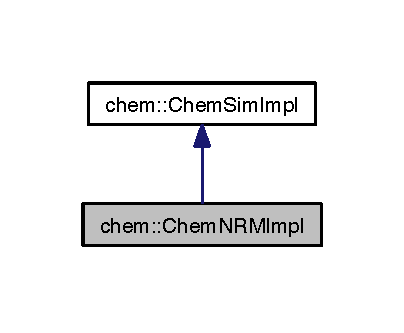
\includegraphics[width=188pt]{classchem_1_1ChemNRMImpl__inherit__graph}
\end{center}
\end{figure}


Collaboration diagram for chem\-:\-:Chem\-N\-R\-M\-Impl\-:\nopagebreak
\begin{figure}[H]
\begin{center}
\leavevmode
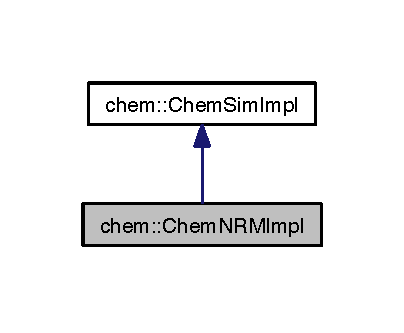
\includegraphics[width=188pt]{classchem_1_1ChemNRMImpl__coll__graph}
\end{center}
\end{figure}
\subsection*{Public Member Functions}
\begin{DoxyCompactItemize}
\item 
\hyperlink{classchem_1_1ChemNRMImpl_ac1d00b6e06300f4959eb7e850a472ab3}{Chem\-N\-R\-M\-Impl} ()
\begin{DoxyCompactList}\small\item\em Ctor\-: Seeds the random number generator, sets global time to 0.\-0 and the number of reactions to 0. \end{DoxyCompactList}\item 
\hyperlink{classchem_1_1ChemNRMImpl_a47d840cba59a2539e65b002a6734f785}{Chem\-N\-R\-M\-Impl} (const \hyperlink{classchem_1_1ChemNRMImpl}{Chem\-N\-R\-M\-Impl} \&rhs)
\begin{DoxyCompactList}\small\item\em Copying is not allowed. \end{DoxyCompactList}\item 
\hyperlink{classchem_1_1ChemNRMImpl}{Chem\-N\-R\-M\-Impl} \& \hyperlink{classchem_1_1ChemNRMImpl_ab9a899fd0d206d67fa30f1aeac103eae}{operator=} (\hyperlink{classchem_1_1ChemNRMImpl}{Chem\-N\-R\-M\-Impl} \&rhs)
\begin{DoxyCompactList}\small\item\em Assignment is not allowed. \end{DoxyCompactList}\item 
virtual \hyperlink{classchem_1_1ChemNRMImpl_a7ce15fefe312380122c36b0860e3014a}{$\sim$\-Chem\-N\-R\-M\-Impl} ()
\begin{DoxyCompactList}\small\item\em Dtor\-: The reaction network is cleared. \end{DoxyCompactList}\item 
size\-\_\-t \hyperlink{classchem_1_1ChemNRMImpl_a0be634b1313bcce9adc160614f34821c}{get\-Size} () const 
\begin{DoxyCompactList}\small\item\em Return the number of reactions in the network. \end{DoxyCompactList}\item 
double \hyperlink{classchem_1_1ChemNRMImpl_accb564d1778f3025c9e9a5a02e7987ec}{get\-Time} () const 
\begin{DoxyCompactList}\small\item\em Return the current global time (as defined in the N\-R\-M algorithm) \end{DoxyCompactList}\item 
void \hyperlink{classchem_1_1ChemNRMImpl_abc38c43b16a4ab1aa31505152e4426ed}{reset\-Time} ()
\begin{DoxyCompactList}\small\item\em Sets global time to 0.\-0. \end{DoxyCompactList}\item 
void \hyperlink{classchem_1_1ChemNRMImpl_ad096a21196bb3e5a978dc3fdb50d8e1b}{sync\-Global\-Time} ()
\begin{DoxyCompactList}\small\item\em Sets global time variable to \hyperlink{classchem_1_1ChemNRMImpl}{Chem\-N\-R\-M\-Impl}'s global time. \end{DoxyCompactList}\item 
\hyperlink{namespacechem_aacd1d2bb93e0bb1b1af9bb1fbb5133ca}{boost\-\_\-heap} $\ast$ \hyperlink{classchem_1_1ChemNRMImpl_ae52572d35469dd8569457dbce96af78e}{get\-Heap} ()
\begin{DoxyCompactList}\small\item\em Return a pointer to the heap. \end{DoxyCompactList}\item 
virtual void \hyperlink{classchem_1_1ChemNRMImpl_a1b325b27b22f443f99fce659ae78aeee}{add\-Reaction} (\hyperlink{classchem_1_1Reaction}{Reaction} $\ast$r)
\begin{DoxyCompactList}\small\item\em Add \hyperlink{classchem_1_1Reaction}{Reaction} $\ast$r to the network. \end{DoxyCompactList}\item 
virtual void \hyperlink{classchem_1_1ChemNRMImpl_ad3a2b84f69c444a55b60d21200537338}{remove\-Reaction} (\hyperlink{classchem_1_1Reaction}{Reaction} $\ast$r)
\begin{DoxyCompactList}\small\item\em Remove \hyperlink{classchem_1_1Reaction}{Reaction} $\ast$r from the network. \end{DoxyCompactList}\item 
double \hyperlink{classchem_1_1ChemNRMImpl_a196f525d2e2392c0531f763fd8169701}{generate\-Tau} (double a)
\begin{DoxyCompactList}\small\item\em A pure function (without sideeffects), which returns a random time tau, drawn from the exponential distribution, with the propensity given by a. \end{DoxyCompactList}\item 
virtual void \hyperlink{classchem_1_1ChemNRMImpl_a685ac34bfa4b8226045bd3b8c6cdec95}{initialize} ()
\begin{DoxyCompactList}\small\item\em This function iterates over all \hyperlink{classchem_1_1RNodeNRM}{R\-Node\-N\-R\-M} objects in the network, generating new tau-\/s for each case and subsequently updating the heap. \end{DoxyCompactList}\item 
virtual bool \hyperlink{classchem_1_1ChemNRMImpl_a236b68389599aa9486959377cfc51496}{run} (int steps)
\begin{DoxyCompactList}\small\item\em This method runs the N\-R\-M algorithm for the given number of steps. \end{DoxyCompactList}\item 
virtual void \hyperlink{classchem_1_1ChemNRMImpl_a7898a5e226789a39b51f8fb56cc85c1e}{print\-Reactions} () const 
\begin{DoxyCompactList}\small\item\em Prints all R\-Nodes in the reaction network. \end{DoxyCompactList}\end{DoxyCompactItemize}
\subsection*{Private Member Functions}
\begin{DoxyCompactItemize}
\item 
bool \hyperlink{classchem_1_1ChemNRMImpl_a9f17d2b5953fd3ffc8b5337e78021ed2}{make\-Step} ()
\begin{DoxyCompactList}\small\item\em This is a somewhat complex subroutine which implements the main part of the Gibson-\/\-Bruck N\-R\-M algoritm. \end{DoxyCompactList}\end{DoxyCompactItemize}
\subsection*{Private Attributes}
\begin{DoxyCompactItemize}
\item 
std\-::unordered\-\_\-map$<$ \hyperlink{classchem_1_1Reaction}{Reaction} \\*
$\ast$, std\-::unique\-\_\-ptr$<$ \hyperlink{classchem_1_1RNodeNRM}{R\-Node\-N\-R\-M} $>$ $>$ \hyperlink{classchem_1_1ChemNRMImpl_a6b86101b0c90389e5f027cc4bffccfd3}{\-\_\-map\-\_\-rnodes}
\begin{DoxyCompactList}\small\item\em The database of \hyperlink{classchem_1_1RNodeNRM}{R\-Node\-N\-R\-M} objects, representing the reaction network. \end{DoxyCompactList}\item 
\hyperlink{namespacechem_aacd1d2bb93e0bb1b1af9bb1fbb5133ca}{boost\-\_\-heap} \hyperlink{classchem_1_1ChemNRMImpl_af2063c9b768c13ac541886947c567c1f}{\-\_\-heap}
\begin{DoxyCompactList}\small\item\em A priority queue for the N\-R\-M algorithm, containing \hyperlink{classchem_1_1PQNode}{P\-Q\-Node} elements. \end{DoxyCompactList}\item 
std\-::mt19937 \hyperlink{classchem_1_1ChemNRMImpl_ad0dce1073a3c37dd21c6523a81dd18e6}{\-\_\-eng}
\begin{DoxyCompactList}\small\item\em Random number generator. \end{DoxyCompactList}\item 
std\-::exponential\-\_\-distribution\\*
$<$ double $>$ \hyperlink{classchem_1_1ChemNRMImpl_ac817f5c731ea5522ea661a9e6c978d6a}{\-\_\-exp\-\_\-distr}
\begin{DoxyCompactList}\small\item\em Adaptor for the exponential distribution. \end{DoxyCompactList}\item 
double \hyperlink{classchem_1_1ChemNRMImpl_a1b14f424d72d3c5b0aafe31d7b7c4f82}{\-\_\-t}
\begin{DoxyCompactList}\small\item\em global time \end{DoxyCompactList}\item 
size\-\_\-t \hyperlink{classchem_1_1ChemNRMImpl_a7e53992b28e926d1a19f3fd7dea171c3}{\-\_\-n\-\_\-reacts}
\begin{DoxyCompactList}\small\item\em number of reactions in the network \end{DoxyCompactList}\end{DoxyCompactItemize}


\subsection{Detailed Description}
\hyperlink{classchem_1_1ChemNRMImpl}{Chem\-N\-R\-M\-Impl} stands for Chemical Next \hyperlink{classchem_1_1Reaction}{Reaction} Method Implementation. 

\hyperlink{classchem_1_1ChemNRMImpl}{Chem\-N\-R\-M\-Impl} manages the N\-R\-M algorithm at the level of the network of reactions. In particular, this class contains the N\-R\-M heap and the exponential random number generator. \hyperlink{classchem_1_1Reaction}{Reaction} objects can be added and removed from the \hyperlink{classchem_1_1ChemNRMImpl}{Chem\-N\-R\-M\-Impl} instance. 

Definition at line 167 of file Chem\-N\-R\-M\-Impl.\-h.



\subsection{Constructor \& Destructor Documentation}
\hypertarget{classchem_1_1ChemNRMImpl_ac1d00b6e06300f4959eb7e850a472ab3}{\index{chem\-::\-Chem\-N\-R\-M\-Impl@{chem\-::\-Chem\-N\-R\-M\-Impl}!Chem\-N\-R\-M\-Impl@{Chem\-N\-R\-M\-Impl}}
\index{Chem\-N\-R\-M\-Impl@{Chem\-N\-R\-M\-Impl}!chem::ChemNRMImpl@{chem\-::\-Chem\-N\-R\-M\-Impl}}
\subsubsection[{Chem\-N\-R\-M\-Impl}]{\setlength{\rightskip}{0pt plus 5cm}{\bf chem\-::\-Chem\-N\-R\-M\-Impl\-::\-Chem\-N\-R\-M\-Impl} (
\begin{DoxyParamCaption}
{}
\end{DoxyParamCaption}
)\hspace{0.3cm}{\ttfamily  \mbox{[}inline\mbox{]}}}}\label{classchem_1_1ChemNRMImpl_ac1d00b6e06300f4959eb7e850a472ab3}


Ctor\-: Seeds the random number generator, sets global time to 0.\-0 and the number of reactions to 0. 



Definition at line 170 of file Chem\-N\-R\-M\-Impl.\-h.



References reset\-Time().

\hypertarget{classchem_1_1ChemNRMImpl_a47d840cba59a2539e65b002a6734f785}{\index{chem\-::\-Chem\-N\-R\-M\-Impl@{chem\-::\-Chem\-N\-R\-M\-Impl}!Chem\-N\-R\-M\-Impl@{Chem\-N\-R\-M\-Impl}}
\index{Chem\-N\-R\-M\-Impl@{Chem\-N\-R\-M\-Impl}!chem::ChemNRMImpl@{chem\-::\-Chem\-N\-R\-M\-Impl}}
\subsubsection[{Chem\-N\-R\-M\-Impl}]{\setlength{\rightskip}{0pt plus 5cm}{\bf chem\-::\-Chem\-N\-R\-M\-Impl\-::\-Chem\-N\-R\-M\-Impl} (
\begin{DoxyParamCaption}
\item[{const {\bf Chem\-N\-R\-M\-Impl} \&}]{rhs}
\end{DoxyParamCaption}
)}}\label{classchem_1_1ChemNRMImpl_a47d840cba59a2539e65b002a6734f785}


Copying is not allowed. 

\hypertarget{classchem_1_1ChemNRMImpl_a7ce15fefe312380122c36b0860e3014a}{\index{chem\-::\-Chem\-N\-R\-M\-Impl@{chem\-::\-Chem\-N\-R\-M\-Impl}!$\sim$\-Chem\-N\-R\-M\-Impl@{$\sim$\-Chem\-N\-R\-M\-Impl}}
\index{$\sim$\-Chem\-N\-R\-M\-Impl@{$\sim$\-Chem\-N\-R\-M\-Impl}!chem::ChemNRMImpl@{chem\-::\-Chem\-N\-R\-M\-Impl}}
\subsubsection[{$\sim$\-Chem\-N\-R\-M\-Impl}]{\setlength{\rightskip}{0pt plus 5cm}{\bf chem\-::\-Chem\-N\-R\-M\-Impl\-::$\sim$\-Chem\-N\-R\-M\-Impl} (
\begin{DoxyParamCaption}
{}
\end{DoxyParamCaption}
)\hspace{0.3cm}{\ttfamily  \mbox{[}virtual\mbox{]}}}}\label{classchem_1_1ChemNRMImpl_a7ce15fefe312380122c36b0860e3014a}


Dtor\-: The reaction network is cleared. 

The \hyperlink{classchem_1_1RNodeNRM}{R\-Node\-N\-R\-M} objects will be destructed, but \hyperlink{classchem_1_1Reaction}{Reaction} objects will stay intact. When the \hyperlink{classchem_1_1RNodeNRM}{R\-Node\-N\-R\-M} objects are destructed, they in turn destruct the corresponding \hyperlink{classchem_1_1PQNode}{P\-Q\-Node} element, setting the \hyperlink{classchem_1_1RNode}{R\-Node} pointer of the \hyperlink{classchem_1_1Reaction}{Reaction} object to null. At the end, the heap itself will go out of scope. 

Definition at line 102 of file Chem\-N\-R\-M\-Impl.\-cpp.



References \-\_\-map\-\_\-rnodes.



\subsection{Member Function Documentation}
\hypertarget{classchem_1_1ChemNRMImpl_a1b325b27b22f443f99fce659ae78aeee}{\index{chem\-::\-Chem\-N\-R\-M\-Impl@{chem\-::\-Chem\-N\-R\-M\-Impl}!add\-Reaction@{add\-Reaction}}
\index{add\-Reaction@{add\-Reaction}!chem::ChemNRMImpl@{chem\-::\-Chem\-N\-R\-M\-Impl}}
\subsubsection[{add\-Reaction}]{\setlength{\rightskip}{0pt plus 5cm}void {\bf chem\-::\-Chem\-N\-R\-M\-Impl\-::add\-Reaction} (
\begin{DoxyParamCaption}
\item[{{\bf Reaction} $\ast$}]{r}
\end{DoxyParamCaption}
)\hspace{0.3cm}{\ttfamily  \mbox{[}virtual\mbox{]}}}}\label{classchem_1_1ChemNRMImpl_a1b325b27b22f443f99fce659ae78aeee}


Add \hyperlink{classchem_1_1Reaction}{Reaction} $\ast$r to the network. 



Implements \hyperlink{classchem_1_1ChemSimImpl_a9000e6ec731865360762f483dd7e91cf}{chem\-::\-Chem\-Sim\-Impl}.



Definition at line 171 of file Chem\-N\-R\-M\-Impl.\-cpp.



References \-\_\-map\-\_\-rnodes, and \-\_\-n\-\_\-reacts.

\hypertarget{classchem_1_1ChemNRMImpl_a196f525d2e2392c0531f763fd8169701}{\index{chem\-::\-Chem\-N\-R\-M\-Impl@{chem\-::\-Chem\-N\-R\-M\-Impl}!generate\-Tau@{generate\-Tau}}
\index{generate\-Tau@{generate\-Tau}!chem::ChemNRMImpl@{chem\-::\-Chem\-N\-R\-M\-Impl}}
\subsubsection[{generate\-Tau}]{\setlength{\rightskip}{0pt plus 5cm}double {\bf chem\-::\-Chem\-N\-R\-M\-Impl\-::generate\-Tau} (
\begin{DoxyParamCaption}
\item[{double}]{a}
\end{DoxyParamCaption}
)}}\label{classchem_1_1ChemNRMImpl_a196f525d2e2392c0531f763fd8169701}


A pure function (without sideeffects), which returns a random time tau, drawn from the exponential distribution, with the propensity given by a. 



Definition at line 106 of file Chem\-N\-R\-M\-Impl.\-cpp.



References \-\_\-eng, and \-\_\-exp\-\_\-distr.



Referenced by chem\-::\-R\-Node\-N\-R\-M\-::generate\-New\-Rand\-Tau().

\hypertarget{classchem_1_1ChemNRMImpl_ae52572d35469dd8569457dbce96af78e}{\index{chem\-::\-Chem\-N\-R\-M\-Impl@{chem\-::\-Chem\-N\-R\-M\-Impl}!get\-Heap@{get\-Heap}}
\index{get\-Heap@{get\-Heap}!chem::ChemNRMImpl@{chem\-::\-Chem\-N\-R\-M\-Impl}}
\subsubsection[{get\-Heap}]{\setlength{\rightskip}{0pt plus 5cm}{\bf boost\-\_\-heap}$\ast$ {\bf chem\-::\-Chem\-N\-R\-M\-Impl\-::get\-Heap} (
\begin{DoxyParamCaption}
{}
\end{DoxyParamCaption}
)\hspace{0.3cm}{\ttfamily  \mbox{[}inline\mbox{]}}}}\label{classchem_1_1ChemNRMImpl_ae52572d35469dd8569457dbce96af78e}


Return a pointer to the heap. 



Definition at line 199 of file Chem\-N\-R\-M\-Impl.\-h.



References \-\_\-heap.



Referenced by chem\-::\-R\-Node\-N\-R\-M\-::\-R\-Node\-N\-R\-M(), chem\-::\-R\-Node\-N\-R\-M\-::update\-Heap(), and chem\-::\-R\-Node\-N\-R\-M\-::$\sim$\-R\-Node\-N\-R\-M().

\hypertarget{classchem_1_1ChemNRMImpl_a0be634b1313bcce9adc160614f34821c}{\index{chem\-::\-Chem\-N\-R\-M\-Impl@{chem\-::\-Chem\-N\-R\-M\-Impl}!get\-Size@{get\-Size}}
\index{get\-Size@{get\-Size}!chem::ChemNRMImpl@{chem\-::\-Chem\-N\-R\-M\-Impl}}
\subsubsection[{get\-Size}]{\setlength{\rightskip}{0pt plus 5cm}size\-\_\-t {\bf chem\-::\-Chem\-N\-R\-M\-Impl\-::get\-Size} (
\begin{DoxyParamCaption}
{}
\end{DoxyParamCaption}
) const\hspace{0.3cm}{\ttfamily  \mbox{[}inline\mbox{]}}}}\label{classchem_1_1ChemNRMImpl_a0be634b1313bcce9adc160614f34821c}


Return the number of reactions in the network. 



Definition at line 187 of file Chem\-N\-R\-M\-Impl.\-h.



References \-\_\-n\-\_\-reacts.

\hypertarget{classchem_1_1ChemNRMImpl_accb564d1778f3025c9e9a5a02e7987ec}{\index{chem\-::\-Chem\-N\-R\-M\-Impl@{chem\-::\-Chem\-N\-R\-M\-Impl}!get\-Time@{get\-Time}}
\index{get\-Time@{get\-Time}!chem::ChemNRMImpl@{chem\-::\-Chem\-N\-R\-M\-Impl}}
\subsubsection[{get\-Time}]{\setlength{\rightskip}{0pt plus 5cm}double {\bf chem\-::\-Chem\-N\-R\-M\-Impl\-::get\-Time} (
\begin{DoxyParamCaption}
{}
\end{DoxyParamCaption}
) const\hspace{0.3cm}{\ttfamily  \mbox{[}inline\mbox{]}}}}\label{classchem_1_1ChemNRMImpl_accb564d1778f3025c9e9a5a02e7987ec}


Return the current global time (as defined in the N\-R\-M algorithm) 



Definition at line 190 of file Chem\-N\-R\-M\-Impl.\-h.



References \-\_\-t.



Referenced by chem\-::\-R\-Node\-N\-R\-M\-::generate\-New\-Rand\-Tau().

\hypertarget{classchem_1_1ChemNRMImpl_a685ac34bfa4b8226045bd3b8c6cdec95}{\index{chem\-::\-Chem\-N\-R\-M\-Impl@{chem\-::\-Chem\-N\-R\-M\-Impl}!initialize@{initialize}}
\index{initialize@{initialize}!chem::ChemNRMImpl@{chem\-::\-Chem\-N\-R\-M\-Impl}}
\subsubsection[{initialize}]{\setlength{\rightskip}{0pt plus 5cm}void {\bf chem\-::\-Chem\-N\-R\-M\-Impl\-::initialize} (
\begin{DoxyParamCaption}
{}
\end{DoxyParamCaption}
)\hspace{0.3cm}{\ttfamily  \mbox{[}virtual\mbox{]}}}}\label{classchem_1_1ChemNRMImpl_a685ac34bfa4b8226045bd3b8c6cdec95}


This function iterates over all \hyperlink{classchem_1_1RNodeNRM}{R\-Node\-N\-R\-M} objects in the network, generating new tau-\/s for each case and subsequently updating the heap. 

It needs to be called before calling run(...). \begin{DoxyNote}{Note}
If somewhere in the middle of simulaiton \hyperlink{classchem_1_1ChemNRMImpl_a685ac34bfa4b8226045bd3b8c6cdec95}{initialize()} is called, it will be analogous to starting the simulation from scratch, except with the \hyperlink{classchem_1_1Species}{Species} copy numbers given at that moment in time. The global time is reset to zero again. 
\end{DoxyNote}


Implements \hyperlink{classchem_1_1ChemSimImpl_a250b43230ac66832bbcecf4f630f2fbc}{chem\-::\-Chem\-Sim\-Impl}.



Definition at line 93 of file Chem\-N\-R\-M\-Impl.\-cpp.



References \-\_\-map\-\_\-rnodes, and reset\-Time().

\hypertarget{classchem_1_1ChemNRMImpl_a9f17d2b5953fd3ffc8b5337e78021ed2}{\index{chem\-::\-Chem\-N\-R\-M\-Impl@{chem\-::\-Chem\-N\-R\-M\-Impl}!make\-Step@{make\-Step}}
\index{make\-Step@{make\-Step}!chem::ChemNRMImpl@{chem\-::\-Chem\-N\-R\-M\-Impl}}
\subsubsection[{make\-Step}]{\setlength{\rightskip}{0pt plus 5cm}bool {\bf chem\-::\-Chem\-N\-R\-M\-Impl\-::make\-Step} (
\begin{DoxyParamCaption}
{}
\end{DoxyParamCaption}
)\hspace{0.3cm}{\ttfamily  \mbox{[}private\mbox{]}}}}\label{classchem_1_1ChemNRMImpl_a9f17d2b5953fd3ffc8b5337e78021ed2}


This is a somewhat complex subroutine which implements the main part of the Gibson-\/\-Bruck N\-R\-M algoritm. 

See the implementation for details. After this method returns, roughly the following will have happened\-: 1) The \hyperlink{classchem_1_1Reaction}{Reaction} corresponding to the lowest tau \hyperlink{classchem_1_1RNodeNRM}{R\-Node\-N\-R\-M} is executed and the corresponding \hyperlink{classchem_1_1Species}{Species} copy numbers are changed 2) A new tau is computed from this \hyperlink{classchem_1_1Reaction}{Reaction} and the corresponding \hyperlink{classchem_1_1PQNode}{P\-Q\-Node} element is updated in the heap 3) The other affected \hyperlink{classchem_1_1Reaction}{Reaction} objects are found, their taus are recomputed and corresponding \hyperlink{classchem_1_1PQNode}{P\-Q\-Node} elements are updated in the heap. 4) For the \hyperlink{classchem_1_1Reaction}{Reaction} and associated \hyperlink{classchem_1_1Species}{Species} signals are emitted, if these objects broadcast signals upon change. Returns true if successful, and false if the heap is exchausted and there no more reactions to fire 

Definition at line 112 of file Chem\-N\-R\-M\-Impl.\-cpp.



References \-\_\-heap, \-\_\-t, chem\-::\-Reaction\-::begin\-Products(), chem\-::\-Reaction\-::begin\-Reactants(), chem\-::\-Reaction\-::dependents(), chem\-::\-Reaction\-::emit\-Signal(), chem\-::\-Reaction\-::end\-Products(), chem\-::\-Reaction\-::end\-Reactants(), chem\-::\-R\-Node\-N\-R\-M\-::generate\-New\-Rand\-Tau(), chem\-::\-R\-Node\-N\-R\-M\-::get\-Propensity(), chem\-::\-R\-Node\-N\-R\-M\-::get\-Reaction(), chem\-::\-R\-Node\-N\-R\-M\-::get\-Tau(), chem\-::\-R\-Node\-N\-R\-M\-::is\-Passivated(), chem\-::\-R\-Node\-N\-R\-M\-::make\-Step(), chem\-::\-R\-Node\-N\-R\-M\-::re\-Compute\-Propensity(), chem\-::\-R\-Node\-N\-R\-M\-::set\-Tau(), sync\-Global\-Time(), and chem\-::\-R\-Node\-N\-R\-M\-::update\-Heap().



Referenced by run().

\hypertarget{classchem_1_1ChemNRMImpl_ab9a899fd0d206d67fa30f1aeac103eae}{\index{chem\-::\-Chem\-N\-R\-M\-Impl@{chem\-::\-Chem\-N\-R\-M\-Impl}!operator=@{operator=}}
\index{operator=@{operator=}!chem::ChemNRMImpl@{chem\-::\-Chem\-N\-R\-M\-Impl}}
\subsubsection[{operator=}]{\setlength{\rightskip}{0pt plus 5cm}{\bf Chem\-N\-R\-M\-Impl}\& chem\-::\-Chem\-N\-R\-M\-Impl\-::operator= (
\begin{DoxyParamCaption}
\item[{{\bf Chem\-N\-R\-M\-Impl} \&}]{rhs}
\end{DoxyParamCaption}
)}}\label{classchem_1_1ChemNRMImpl_ab9a899fd0d206d67fa30f1aeac103eae}


Assignment is not allowed. 

\hypertarget{classchem_1_1ChemNRMImpl_a7898a5e226789a39b51f8fb56cc85c1e}{\index{chem\-::\-Chem\-N\-R\-M\-Impl@{chem\-::\-Chem\-N\-R\-M\-Impl}!print\-Reactions@{print\-Reactions}}
\index{print\-Reactions@{print\-Reactions}!chem::ChemNRMImpl@{chem\-::\-Chem\-N\-R\-M\-Impl}}
\subsubsection[{print\-Reactions}]{\setlength{\rightskip}{0pt plus 5cm}void {\bf chem\-::\-Chem\-N\-R\-M\-Impl\-::print\-Reactions} (
\begin{DoxyParamCaption}
{}
\end{DoxyParamCaption}
) const\hspace{0.3cm}{\ttfamily  \mbox{[}virtual\mbox{]}}}}\label{classchem_1_1ChemNRMImpl_a7898a5e226789a39b51f8fb56cc85c1e}


Prints all R\-Nodes in the reaction network. 



Implements \hyperlink{classchem_1_1ChemSimImpl_a24291dac40633358ab6a9f473d6f861d}{chem\-::\-Chem\-Sim\-Impl}.



Definition at line 181 of file Chem\-N\-R\-M\-Impl.\-cpp.



References \-\_\-map\-\_\-rnodes.

\hypertarget{classchem_1_1ChemNRMImpl_ad3a2b84f69c444a55b60d21200537338}{\index{chem\-::\-Chem\-N\-R\-M\-Impl@{chem\-::\-Chem\-N\-R\-M\-Impl}!remove\-Reaction@{remove\-Reaction}}
\index{remove\-Reaction@{remove\-Reaction}!chem::ChemNRMImpl@{chem\-::\-Chem\-N\-R\-M\-Impl}}
\subsubsection[{remove\-Reaction}]{\setlength{\rightskip}{0pt plus 5cm}void {\bf chem\-::\-Chem\-N\-R\-M\-Impl\-::remove\-Reaction} (
\begin{DoxyParamCaption}
\item[{{\bf Reaction} $\ast$}]{r}
\end{DoxyParamCaption}
)\hspace{0.3cm}{\ttfamily  \mbox{[}virtual\mbox{]}}}}\label{classchem_1_1ChemNRMImpl_ad3a2b84f69c444a55b60d21200537338}


Remove \hyperlink{classchem_1_1Reaction}{Reaction} $\ast$r from the network. 



Implements \hyperlink{classchem_1_1ChemSimImpl_a00e43cfb099cb26e44d04a715b6cba0a}{chem\-::\-Chem\-Sim\-Impl}.



Definition at line 176 of file Chem\-N\-R\-M\-Impl.\-cpp.



References \-\_\-map\-\_\-rnodes, and \-\_\-n\-\_\-reacts.

\hypertarget{classchem_1_1ChemNRMImpl_abc38c43b16a4ab1aa31505152e4426ed}{\index{chem\-::\-Chem\-N\-R\-M\-Impl@{chem\-::\-Chem\-N\-R\-M\-Impl}!reset\-Time@{reset\-Time}}
\index{reset\-Time@{reset\-Time}!chem::ChemNRMImpl@{chem\-::\-Chem\-N\-R\-M\-Impl}}
\subsubsection[{reset\-Time}]{\setlength{\rightskip}{0pt plus 5cm}void {\bf chem\-::\-Chem\-N\-R\-M\-Impl\-::reset\-Time} (
\begin{DoxyParamCaption}
{}
\end{DoxyParamCaption}
)\hspace{0.3cm}{\ttfamily  \mbox{[}inline\mbox{]}}}}\label{classchem_1_1ChemNRMImpl_abc38c43b16a4ab1aa31505152e4426ed}


Sets global time to 0.\-0. 



Definition at line 193 of file Chem\-N\-R\-M\-Impl.\-h.



References \-\_\-t, and sync\-Global\-Time().



Referenced by Chem\-N\-R\-M\-Impl(), and initialize().

\hypertarget{classchem_1_1ChemNRMImpl_a236b68389599aa9486959377cfc51496}{\index{chem\-::\-Chem\-N\-R\-M\-Impl@{chem\-::\-Chem\-N\-R\-M\-Impl}!run@{run}}
\index{run@{run}!chem::ChemNRMImpl@{chem\-::\-Chem\-N\-R\-M\-Impl}}
\subsubsection[{run}]{\setlength{\rightskip}{0pt plus 5cm}virtual bool {\bf chem\-::\-Chem\-N\-R\-M\-Impl\-::run} (
\begin{DoxyParamCaption}
\item[{int}]{steps}
\end{DoxyParamCaption}
)\hspace{0.3cm}{\ttfamily  \mbox{[}inline, virtual\mbox{]}}}}\label{classchem_1_1ChemNRMImpl_a236b68389599aa9486959377cfc51496}


This method runs the N\-R\-M algorithm for the given number of steps. 



Implements \hyperlink{classchem_1_1ChemSimImpl_a9f051e00a754fdd76d5e2b3a217f3a49}{chem\-::\-Chem\-Sim\-Impl}.



Definition at line 219 of file Chem\-N\-R\-M\-Impl.\-h.



References make\-Step().

\hypertarget{classchem_1_1ChemNRMImpl_ad096a21196bb3e5a978dc3fdb50d8e1b}{\index{chem\-::\-Chem\-N\-R\-M\-Impl@{chem\-::\-Chem\-N\-R\-M\-Impl}!sync\-Global\-Time@{sync\-Global\-Time}}
\index{sync\-Global\-Time@{sync\-Global\-Time}!chem::ChemNRMImpl@{chem\-::\-Chem\-N\-R\-M\-Impl}}
\subsubsection[{sync\-Global\-Time}]{\setlength{\rightskip}{0pt plus 5cm}void {\bf chem\-::\-Chem\-N\-R\-M\-Impl\-::sync\-Global\-Time} (
\begin{DoxyParamCaption}
{}
\end{DoxyParamCaption}
)\hspace{0.3cm}{\ttfamily  \mbox{[}inline\mbox{]}}}}\label{classchem_1_1ChemNRMImpl_ad096a21196bb3e5a978dc3fdb50d8e1b}


Sets global time variable to \hyperlink{classchem_1_1ChemNRMImpl}{Chem\-N\-R\-M\-Impl}'s global time. 



Definition at line 196 of file Chem\-N\-R\-M\-Impl.\-h.



References \-\_\-t, and global\-\_\-time.



Referenced by make\-Step(), and reset\-Time().



\subsection{Member Data Documentation}
\hypertarget{classchem_1_1ChemNRMImpl_ad0dce1073a3c37dd21c6523a81dd18e6}{\index{chem\-::\-Chem\-N\-R\-M\-Impl@{chem\-::\-Chem\-N\-R\-M\-Impl}!\-\_\-eng@{\-\_\-eng}}
\index{\-\_\-eng@{\-\_\-eng}!chem::ChemNRMImpl@{chem\-::\-Chem\-N\-R\-M\-Impl}}
\subsubsection[{\-\_\-eng}]{\setlength{\rightskip}{0pt plus 5cm}std\-::mt19937 {\bf chem\-::\-Chem\-N\-R\-M\-Impl\-::\-\_\-eng}\hspace{0.3cm}{\ttfamily  \mbox{[}private\mbox{]}}}}\label{classchem_1_1ChemNRMImpl_ad0dce1073a3c37dd21c6523a81dd18e6}


Random number generator. 



Definition at line 246 of file Chem\-N\-R\-M\-Impl.\-h.



Referenced by generate\-Tau().

\hypertarget{classchem_1_1ChemNRMImpl_ac817f5c731ea5522ea661a9e6c978d6a}{\index{chem\-::\-Chem\-N\-R\-M\-Impl@{chem\-::\-Chem\-N\-R\-M\-Impl}!\-\_\-exp\-\_\-distr@{\-\_\-exp\-\_\-distr}}
\index{\-\_\-exp\-\_\-distr@{\-\_\-exp\-\_\-distr}!chem::ChemNRMImpl@{chem\-::\-Chem\-N\-R\-M\-Impl}}
\subsubsection[{\-\_\-exp\-\_\-distr}]{\setlength{\rightskip}{0pt plus 5cm}std\-::exponential\-\_\-distribution$<$double$>$ {\bf chem\-::\-Chem\-N\-R\-M\-Impl\-::\-\_\-exp\-\_\-distr}\hspace{0.3cm}{\ttfamily  \mbox{[}private\mbox{]}}}}\label{classchem_1_1ChemNRMImpl_ac817f5c731ea5522ea661a9e6c978d6a}


Adaptor for the exponential distribution. 



Definition at line 247 of file Chem\-N\-R\-M\-Impl.\-h.



Referenced by generate\-Tau().

\hypertarget{classchem_1_1ChemNRMImpl_af2063c9b768c13ac541886947c567c1f}{\index{chem\-::\-Chem\-N\-R\-M\-Impl@{chem\-::\-Chem\-N\-R\-M\-Impl}!\-\_\-heap@{\-\_\-heap}}
\index{\-\_\-heap@{\-\_\-heap}!chem::ChemNRMImpl@{chem\-::\-Chem\-N\-R\-M\-Impl}}
\subsubsection[{\-\_\-heap}]{\setlength{\rightskip}{0pt plus 5cm}{\bf boost\-\_\-heap} {\bf chem\-::\-Chem\-N\-R\-M\-Impl\-::\-\_\-heap}\hspace{0.3cm}{\ttfamily  \mbox{[}private\mbox{]}}}}\label{classchem_1_1ChemNRMImpl_af2063c9b768c13ac541886947c567c1f}


A priority queue for the N\-R\-M algorithm, containing \hyperlink{classchem_1_1PQNode}{P\-Q\-Node} elements. 



Definition at line 245 of file Chem\-N\-R\-M\-Impl.\-h.



Referenced by get\-Heap(), and make\-Step().

\hypertarget{classchem_1_1ChemNRMImpl_a6b86101b0c90389e5f027cc4bffccfd3}{\index{chem\-::\-Chem\-N\-R\-M\-Impl@{chem\-::\-Chem\-N\-R\-M\-Impl}!\-\_\-map\-\_\-rnodes@{\-\_\-map\-\_\-rnodes}}
\index{\-\_\-map\-\_\-rnodes@{\-\_\-map\-\_\-rnodes}!chem::ChemNRMImpl@{chem\-::\-Chem\-N\-R\-M\-Impl}}
\subsubsection[{\-\_\-map\-\_\-rnodes}]{\setlength{\rightskip}{0pt plus 5cm}std\-::unordered\-\_\-map$<${\bf Reaction}$\ast$, std\-::unique\-\_\-ptr$<${\bf R\-Node\-N\-R\-M}$>$ $>$ {\bf chem\-::\-Chem\-N\-R\-M\-Impl\-::\-\_\-map\-\_\-rnodes}\hspace{0.3cm}{\ttfamily  \mbox{[}private\mbox{]}}}}\label{classchem_1_1ChemNRMImpl_a6b86101b0c90389e5f027cc4bffccfd3}


The database of \hyperlink{classchem_1_1RNodeNRM}{R\-Node\-N\-R\-M} objects, representing the reaction network. 



Definition at line 244 of file Chem\-N\-R\-M\-Impl.\-h.



Referenced by add\-Reaction(), initialize(), print\-Reactions(), remove\-Reaction(), and $\sim$\-Chem\-N\-R\-M\-Impl().

\hypertarget{classchem_1_1ChemNRMImpl_a7e53992b28e926d1a19f3fd7dea171c3}{\index{chem\-::\-Chem\-N\-R\-M\-Impl@{chem\-::\-Chem\-N\-R\-M\-Impl}!\-\_\-n\-\_\-reacts@{\-\_\-n\-\_\-reacts}}
\index{\-\_\-n\-\_\-reacts@{\-\_\-n\-\_\-reacts}!chem::ChemNRMImpl@{chem\-::\-Chem\-N\-R\-M\-Impl}}
\subsubsection[{\-\_\-n\-\_\-reacts}]{\setlength{\rightskip}{0pt plus 5cm}size\-\_\-t {\bf chem\-::\-Chem\-N\-R\-M\-Impl\-::\-\_\-n\-\_\-reacts}\hspace{0.3cm}{\ttfamily  \mbox{[}private\mbox{]}}}}\label{classchem_1_1ChemNRMImpl_a7e53992b28e926d1a19f3fd7dea171c3}


number of reactions in the network 



Definition at line 249 of file Chem\-N\-R\-M\-Impl.\-h.



Referenced by add\-Reaction(), get\-Size(), and remove\-Reaction().

\hypertarget{classchem_1_1ChemNRMImpl_a1b14f424d72d3c5b0aafe31d7b7c4f82}{\index{chem\-::\-Chem\-N\-R\-M\-Impl@{chem\-::\-Chem\-N\-R\-M\-Impl}!\-\_\-t@{\-\_\-t}}
\index{\-\_\-t@{\-\_\-t}!chem::ChemNRMImpl@{chem\-::\-Chem\-N\-R\-M\-Impl}}
\subsubsection[{\-\_\-t}]{\setlength{\rightskip}{0pt plus 5cm}double {\bf chem\-::\-Chem\-N\-R\-M\-Impl\-::\-\_\-t}\hspace{0.3cm}{\ttfamily  \mbox{[}private\mbox{]}}}}\label{classchem_1_1ChemNRMImpl_a1b14f424d72d3c5b0aafe31d7b7c4f82}


global time 



Definition at line 248 of file Chem\-N\-R\-M\-Impl.\-h.



Referenced by get\-Time(), make\-Step(), reset\-Time(), and sync\-Global\-Time().



The documentation for this class was generated from the following files\-:\begin{DoxyCompactItemize}
\item 
Cyto\-Sim/\hyperlink{ChemNRMImpl_8h}{Chem\-N\-R\-M\-Impl.\-h}\item 
Cyto\-Sim/\hyperlink{ChemNRMImpl_8cpp}{Chem\-N\-R\-M\-Impl.\-cpp}\end{DoxyCompactItemize}

\hypertarget{classchem_1_1ChemSignal}{\section{chem\-:\-:Chem\-Signal Class Reference}
\label{classchem_1_1ChemSignal}\index{chem\-::\-Chem\-Signal@{chem\-::\-Chem\-Signal}}
}


\hyperlink{classchem_1_1ChemSignal}{Chem\-Signal} manages callbacks for \hyperlink{classchem_1_1RSpecies}{R\-Species} and Reactions objects.  




{\ttfamily \#include $<$Signaling.\-h$>$}

\subsection*{Public Member Functions}
\begin{DoxyCompactItemize}
\item 
void \hyperlink{classchem_1_1ChemSignal_a1ce27770cc3ce07fc96d558933bc20f9}{emit\-Reaction\-Signal} (\hyperlink{classchem_1_1ReactionBase}{Reaction\-Base} $\ast$r) const 
\begin{DoxyCompactList}\small\item\em Broadcasts signal corresponding to \hyperlink{classchem_1_1ReactionBase}{Reaction\-Base} $\ast$r. \end{DoxyCompactList}\item 
void \hyperlink{classchem_1_1ChemSignal_ab27c28368d6fab40f2d50129108a15bc}{emit\-R\-Species\-Signal} (\hyperlink{classchem_1_1RSpecies}{R\-Species} $\ast$s, int delta) const 
\begin{DoxyCompactList}\small\item\em Broadcasts signal corresponding to \hyperlink{classchem_1_1RSpecies}{R\-Species} $\ast$s. \end{DoxyCompactList}\item 
void \hyperlink{classchem_1_1ChemSignal_a9c370cbe1e3376366c95e95c4aa512e9}{add\-Signaling\-R\-Species} (\hyperlink{classchem_1_1RSpecies}{R\-Species} $\ast$s)
\begin{DoxyCompactList}\small\item\em Inserts a signal corresponding to \hyperlink{classchem_1_1RSpecies}{R\-Species} $\ast$s into the map. \end{DoxyCompactList}\item 
void \hyperlink{classchem_1_1ChemSignal_a67eacb25dd81028c18c48872bef3b1fe}{add\-Signaling\-Reaction} (\hyperlink{classchem_1_1ReactionBase}{Reaction\-Base} $\ast$r)
\begin{DoxyCompactList}\small\item\em Inserts a signal corresponding to \hyperlink{classchem_1_1ReactionBase}{Reaction\-Base} $\ast$r into the map. \end{DoxyCompactList}\item 
boost\-::signals2\-::connection \hyperlink{classchem_1_1ChemSignal_a698e5c6577fae437828ac52238bf0ba0}{connect} (\hyperlink{classchem_1_1ReactionBase}{Reaction\-Base} $\ast$r, std\-::function$<$ void(\hyperlink{classchem_1_1ReactionBase}{Reaction\-Base} $\ast$)$>$ const \&react\-\_\-callback, int priority=5)
\begin{DoxyCompactList}\small\item\em Connect the callback, react\-\_\-callback to a signal corresponding to \hyperlink{classchem_1_1ReactionBase}{Reaction\-Base} $\ast$r. \end{DoxyCompactList}\item 
boost\-::signals2\-::connection \hyperlink{classchem_1_1ChemSignal_a74cb3a95f3f9793f4a0343180aa01074}{connect} (\hyperlink{classchem_1_1Species}{Species} $\ast$s, std\-::function$<$ void(\hyperlink{classchem_1_1RSpecies}{R\-Species} $\ast$, int)$>$ const \&R\-Species\-\_\-callback, int priority=5)
\begin{DoxyCompactList}\small\item\em Connect the callback, R\-Species\-\_\-callback to a signal corresponding to \hyperlink{classchem_1_1RSpecies}{R\-Species} $\ast$s. \end{DoxyCompactList}\item 
void \hyperlink{classchem_1_1ChemSignal_ac1484774e9bf4a0e93999a4061d5a97c}{disconnect} (\hyperlink{classchem_1_1ReactionBase}{Reaction\-Base} $\ast$r)
\begin{DoxyCompactList}\small\item\em Destroy signal corresponding to \hyperlink{classchem_1_1Reaction}{Reaction} r. \end{DoxyCompactList}\item 
void \hyperlink{classchem_1_1ChemSignal_a546b0feb4e8a50ae0e3833ede8d9faee}{disconnect} (\hyperlink{classchem_1_1RSpecies}{R\-Species} $\ast$s)
\begin{DoxyCompactList}\small\item\em Destroy signal corresponding to \hyperlink{classchem_1_1Reaction}{Reaction} r. \end{DoxyCompactList}\end{DoxyCompactItemize}
\subsection*{Private Member Functions}
\begin{DoxyCompactItemize}
\item 
std\-::unordered\-\_\-map\\*
$<$ \hyperlink{classchem_1_1ReactionBase}{Reaction\-Base} \\*
$\ast$, std\-::unique\-\_\-ptr\\*
$<$ \hyperlink{namespacechem_a40bfcc5c8ae87e2713c68fae68215991}{Reaction\-Event\-Signal} $>$\\*
 $>$\-::const\-\_\-iterator \hyperlink{classchem_1_1ChemSignal_ac988afbd07af10fb3fc72f688adaef5e}{find\-Signal} (\hyperlink{classchem_1_1ReactionBase}{Reaction\-Base} $\ast$r) const 
\begin{DoxyCompactList}\small\item\em Search the map for a signal corresponding to parameter, \hyperlink{classchem_1_1ReactionBase}{Reaction\-Base} $\ast$r. Throw std\-::out\-\_\-of\-\_\-range exception if not found. \end{DoxyCompactList}\item 
std\-::unordered\-\_\-map$<$ \hyperlink{classchem_1_1RSpecies}{R\-Species} \\*
$\ast$, std\-::unique\-\_\-ptr\\*
$<$ \hyperlink{namespacechem_a6cb4144586460e7b7ae0dffdf08eb57c}{R\-Species\-Copy\-N\-Changed\-Signal} $>$\\*
 $>$\-::const\-\_\-iterator \hyperlink{classchem_1_1ChemSignal_ae10bf98b41aa071c0595c9ae2c320858}{find\-Signal} (\hyperlink{classchem_1_1RSpecies}{R\-Species} $\ast$s) const 
\begin{DoxyCompactList}\small\item\em Search the map for a signal corresponding to parameter, \hyperlink{classchem_1_1RSpecies}{R\-Species} $\ast$s. Throw std\-::out\-\_\-of\-\_\-range exception if not found. \end{DoxyCompactList}\item 
void \hyperlink{classchem_1_1ChemSignal_ae823c2e49c5dcd6eefe8e44d8628622a}{assert\-Signal\-Does\-Not\-Exist} (\hyperlink{classchem_1_1ReactionBase}{Reaction\-Base} $\ast$r)
\begin{DoxyCompactList}\small\item\em Assert that a signal corresponding to \hyperlink{classchem_1_1ReactionBase}{Reaction\-Base} $\ast$r does not exist or throw std\-::runtime\-\_\-error. \end{DoxyCompactList}\item 
void \hyperlink{classchem_1_1ChemSignal_a20c30365e810b3b88e87500e08627d11}{assert\-Signal\-Does\-Not\-Exist} (\hyperlink{classchem_1_1RSpecies}{R\-Species} $\ast$s)
\begin{DoxyCompactList}\small\item\em Assert that a signal corresponding to \hyperlink{classchem_1_1RSpecies}{R\-Species} $\ast$s does not exist or throw std\-::runtime\-\_\-error. \end{DoxyCompactList}\end{DoxyCompactItemize}
\subsection*{Private Attributes}
\begin{DoxyCompactItemize}
\item 
std\-::unordered\-\_\-map$<$ \hyperlink{classchem_1_1RSpecies}{R\-Species} \\*
$\ast$, std\-::unique\-\_\-ptr\\*
$<$ \hyperlink{namespacechem_a6cb4144586460e7b7ae0dffdf08eb57c}{R\-Species\-Copy\-N\-Changed\-Signal} $>$ $>$ \hyperlink{classchem_1_1ChemSignal_a7721fb9395d65c7de08108163a3d4cdb}{\-\_\-map\-\_\-\-R\-Species\-\_\-signal}
\begin{DoxyCompactList}\small\item\em Keep track of signals corresponding to various \hyperlink{classchem_1_1RSpecies}{R\-Species}. \end{DoxyCompactList}\item 
std\-::unordered\-\_\-map\\*
$<$ \hyperlink{classchem_1_1ReactionBase}{Reaction\-Base} \\*
$\ast$, std\-::unique\-\_\-ptr\\*
$<$ \hyperlink{namespacechem_a40bfcc5c8ae87e2713c68fae68215991}{Reaction\-Event\-Signal} $>$ $>$ \hyperlink{classchem_1_1ChemSignal_a5a8fb8af001c1575256ee7b671c42ea3}{\-\_\-map\-\_\-reaction\-\_\-signal}
\begin{DoxyCompactList}\small\item\em Keep track of signals corresponding to various Reactions. \end{DoxyCompactList}\end{DoxyCompactItemize}


\subsection{Detailed Description}
\hyperlink{classchem_1_1ChemSignal}{Chem\-Signal} manages callbacks for \hyperlink{classchem_1_1RSpecies}{R\-Species} and Reactions objects. 

One \hyperlink{classchem_1_1ChemSignal}{Chem\-Signal} should be instantiated per chemical network. \hyperlink{classchem_1_1RSpecies}{R\-Species} and Reactions that need to be monitored can be made to signal, based on the boost\-:signal2 library. Multiple receiving slots can be connected to signals.

Slots can be temporarily blocked or completely disconnected. Signals can be destroyed. Here is an example of usage\-: 
\begin{DoxyCode}
 ...
 Species* A1 = ...
 ...
 ChemSignal sm;
 A1->makeSignaling(sm);
 PrintRSpecies ps;
 ...
 std::function<void (RSpecies *, int)> psf(ps);
 boost::signals2::shared_connection_block conn_a1(sm.connect(A1, [](RSpecies *s
      , int i){s->printSelf();}), true);
 // or   sm.connect(A1, print_RSpecies);
 // or  sm.connect(A1, PrintRSpecies());
 // or   boost::signals2::shared_connection_block conn_a1(sm.connect(A1,psf),
       false);
...
// run simulation for some time
 ...
 conn_a1.block(); // this temporarily stops slots from being called.
...
 conn_a1.disconnect(); // this permanently disconnects the slot
...
 A1->stopSignaling(sm); // this destroys the Signal itself (with associated
       multiple slots)
...
\end{DoxyCode}
 

Definition at line 66 of file Signaling.\-h.



\subsection{Member Function Documentation}
\hypertarget{classchem_1_1ChemSignal_a67eacb25dd81028c18c48872bef3b1fe}{\index{chem\-::\-Chem\-Signal@{chem\-::\-Chem\-Signal}!add\-Signaling\-Reaction@{add\-Signaling\-Reaction}}
\index{add\-Signaling\-Reaction@{add\-Signaling\-Reaction}!chem::ChemSignal@{chem\-::\-Chem\-Signal}}
\subsubsection[{add\-Signaling\-Reaction}]{\setlength{\rightskip}{0pt plus 5cm}void {\bf chem\-::\-Chem\-Signal\-::add\-Signaling\-Reaction} (
\begin{DoxyParamCaption}
\item[{{\bf Reaction\-Base} $\ast$}]{r}
\end{DoxyParamCaption}
)\hspace{0.3cm}{\ttfamily  \mbox{[}inline\mbox{]}}}}\label{classchem_1_1ChemSignal_a67eacb25dd81028c18c48872bef3b1fe}


Inserts a signal corresponding to \hyperlink{classchem_1_1ReactionBase}{Reaction\-Base} $\ast$r into the map. 

Should only be called by the \hyperlink{classchem_1_1Reaction}{Reaction} class. \begin{DoxyNote}{Note}
other classes should instead call void Reaction\-::make\-Signaling(\-Chem\-Signal \&sm); 
\end{DoxyNote}


Definition at line 128 of file Signaling.\-h.



References \-\_\-map\-\_\-reaction\-\_\-signal, and assert\-Signal\-Does\-Not\-Exist().

\hypertarget{classchem_1_1ChemSignal_a9c370cbe1e3376366c95e95c4aa512e9}{\index{chem\-::\-Chem\-Signal@{chem\-::\-Chem\-Signal}!add\-Signaling\-R\-Species@{add\-Signaling\-R\-Species}}
\index{add\-Signaling\-R\-Species@{add\-Signaling\-R\-Species}!chem::ChemSignal@{chem\-::\-Chem\-Signal}}
\subsubsection[{add\-Signaling\-R\-Species}]{\setlength{\rightskip}{0pt plus 5cm}void {\bf chem\-::\-Chem\-Signal\-::add\-Signaling\-R\-Species} (
\begin{DoxyParamCaption}
\item[{{\bf R\-Species} $\ast$}]{s}
\end{DoxyParamCaption}
)\hspace{0.3cm}{\ttfamily  \mbox{[}inline\mbox{]}}}}\label{classchem_1_1ChemSignal_a9c370cbe1e3376366c95e95c4aa512e9}


Inserts a signal corresponding to \hyperlink{classchem_1_1RSpecies}{R\-Species} $\ast$s into the map. 

Should only be called by the \hyperlink{classchem_1_1RSpecies}{R\-Species} class. \begin{DoxyNote}{Note}
other classes should instead call void R\-Species\-::make\-Signaling(\-Chem\-Signal \&sm); 
\end{DoxyNote}


Definition at line 120 of file Signaling.\-h.



References \-\_\-map\-\_\-\-R\-Species\-\_\-signal, and assert\-Signal\-Does\-Not\-Exist().

\hypertarget{classchem_1_1ChemSignal_ae823c2e49c5dcd6eefe8e44d8628622a}{\index{chem\-::\-Chem\-Signal@{chem\-::\-Chem\-Signal}!assert\-Signal\-Does\-Not\-Exist@{assert\-Signal\-Does\-Not\-Exist}}
\index{assert\-Signal\-Does\-Not\-Exist@{assert\-Signal\-Does\-Not\-Exist}!chem::ChemSignal@{chem\-::\-Chem\-Signal}}
\subsubsection[{assert\-Signal\-Does\-Not\-Exist}]{\setlength{\rightskip}{0pt plus 5cm}void {\bf chem\-::\-Chem\-Signal\-::assert\-Signal\-Does\-Not\-Exist} (
\begin{DoxyParamCaption}
\item[{{\bf Reaction\-Base} $\ast$}]{r}
\end{DoxyParamCaption}
)\hspace{0.3cm}{\ttfamily  \mbox{[}inline, private\mbox{]}}}}\label{classchem_1_1ChemSignal_ae823c2e49c5dcd6eefe8e44d8628622a}


Assert that a signal corresponding to \hyperlink{classchem_1_1ReactionBase}{Reaction\-Base} $\ast$r does not exist or throw std\-::runtime\-\_\-error. 



Definition at line 90 of file Signaling.\-h.



References \-\_\-map\-\_\-reaction\-\_\-signal.



Referenced by add\-Signaling\-Reaction(), and add\-Signaling\-R\-Species().

\hypertarget{classchem_1_1ChemSignal_a20c30365e810b3b88e87500e08627d11}{\index{chem\-::\-Chem\-Signal@{chem\-::\-Chem\-Signal}!assert\-Signal\-Does\-Not\-Exist@{assert\-Signal\-Does\-Not\-Exist}}
\index{assert\-Signal\-Does\-Not\-Exist@{assert\-Signal\-Does\-Not\-Exist}!chem::ChemSignal@{chem\-::\-Chem\-Signal}}
\subsubsection[{assert\-Signal\-Does\-Not\-Exist}]{\setlength{\rightskip}{0pt plus 5cm}void {\bf chem\-::\-Chem\-Signal\-::assert\-Signal\-Does\-Not\-Exist} (
\begin{DoxyParamCaption}
\item[{{\bf R\-Species} $\ast$}]{s}
\end{DoxyParamCaption}
)\hspace{0.3cm}{\ttfamily  \mbox{[}inline, private\mbox{]}}}}\label{classchem_1_1ChemSignal_a20c30365e810b3b88e87500e08627d11}


Assert that a signal corresponding to \hyperlink{classchem_1_1RSpecies}{R\-Species} $\ast$s does not exist or throw std\-::runtime\-\_\-error. 



Definition at line 97 of file Signaling.\-h.



References \-\_\-map\-\_\-\-R\-Species\-\_\-signal.

\hypertarget{classchem_1_1ChemSignal_a698e5c6577fae437828ac52238bf0ba0}{\index{chem\-::\-Chem\-Signal@{chem\-::\-Chem\-Signal}!connect@{connect}}
\index{connect@{connect}!chem::ChemSignal@{chem\-::\-Chem\-Signal}}
\subsubsection[{connect}]{\setlength{\rightskip}{0pt plus 5cm}boost\-::signals2\-::connection {\bf chem\-::\-Chem\-Signal\-::connect} (
\begin{DoxyParamCaption}
\item[{{\bf Reaction\-Base} $\ast$}]{r, }
\item[{std\-::function$<$ void({\bf Reaction\-Base} $\ast$)$>$ const \&}]{react\-\_\-callback, }
\item[{int}]{priority = {\ttfamily 5}}
\end{DoxyParamCaption}
)\hspace{0.3cm}{\ttfamily  \mbox{[}inline\mbox{]}}}}\label{classchem_1_1ChemSignal_a698e5c6577fae437828ac52238bf0ba0}


Connect the callback, react\-\_\-callback to a signal corresponding to \hyperlink{classchem_1_1ReactionBase}{Reaction\-Base} $\ast$r. 


\begin{DoxyParams}{Parameters}
{\em \hyperlink{classchem_1_1ReactionBase}{Reaction\-Base}} & $\ast$r -\/ the signal will correspond to this \hyperlink{classchem_1_1Reaction}{Reaction} \\
\hline
{\em std\-::function$<$void} & (\hyperlink{classchem_1_1ReactionBase}{Reaction\-Base} $\ast$)$>$ const \&react\-\_\-callback -\/ a function object to be called (a slot) \\
\hline
{\em int} & priority -\/ lower priority slots will be called first. Default is 5 Do not use priorities 1 and 2 unless absolutely essential. \\
\hline
\end{DoxyParams}


Definition at line 138 of file Signaling.\-h.



References find\-Signal().

\hypertarget{classchem_1_1ChemSignal_a74cb3a95f3f9793f4a0343180aa01074}{\index{chem\-::\-Chem\-Signal@{chem\-::\-Chem\-Signal}!connect@{connect}}
\index{connect@{connect}!chem::ChemSignal@{chem\-::\-Chem\-Signal}}
\subsubsection[{connect}]{\setlength{\rightskip}{0pt plus 5cm}boost\-::signals2\-::connection {\bf chem\-::\-Chem\-Signal\-::connect} (
\begin{DoxyParamCaption}
\item[{{\bf Species} $\ast$}]{s, }
\item[{std\-::function$<$ void({\bf R\-Species} $\ast$, int)$>$ const \&}]{R\-Species\-\_\-callback, }
\item[{int}]{priority = {\ttfamily 5}}
\end{DoxyParamCaption}
)\hspace{0.3cm}{\ttfamily  \mbox{[}inline\mbox{]}}}}\label{classchem_1_1ChemSignal_a74cb3a95f3f9793f4a0343180aa01074}


Connect the callback, R\-Species\-\_\-callback to a signal corresponding to \hyperlink{classchem_1_1RSpecies}{R\-Species} $\ast$s. 


\begin{DoxyParams}{Parameters}
{\em \hyperlink{classchem_1_1RSpecies}{R\-Species}} & $\ast$s -\/ the signal will correspond to this \hyperlink{classchem_1_1RSpecies}{R\-Species} \\
\hline
{\em std\-::function$<$void} & (\hyperlink{classchem_1_1RSpecies}{R\-Species} $\ast$, int)$>$ const \&R\-Species\-\_\-callback -\/ a function object to be called (a slot). int here corresponds to delta, the change in copy number of the \hyperlink{classchem_1_1RSpecies}{R\-Species} (for which the signal was emitted) \\
\hline
{\em int} & priority -\/ lower priority slots will be called first. Default is 5 Do not use priorities 1 and 2 unless absolutely essential. \\
\hline
\end{DoxyParams}


Definition at line 149 of file Signaling.\-h.



References find\-Signal(), and chem\-::\-Species\-::get\-R\-Species().

\hypertarget{classchem_1_1ChemSignal_ac1484774e9bf4a0e93999a4061d5a97c}{\index{chem\-::\-Chem\-Signal@{chem\-::\-Chem\-Signal}!disconnect@{disconnect}}
\index{disconnect@{disconnect}!chem::ChemSignal@{chem\-::\-Chem\-Signal}}
\subsubsection[{disconnect}]{\setlength{\rightskip}{0pt plus 5cm}void {\bf chem\-::\-Chem\-Signal\-::disconnect} (
\begin{DoxyParamCaption}
\item[{{\bf Reaction\-Base} $\ast$}]{r}
\end{DoxyParamCaption}
)\hspace{0.3cm}{\ttfamily  \mbox{[}inline\mbox{]}}}}\label{classchem_1_1ChemSignal_ac1484774e9bf4a0e93999a4061d5a97c}


Destroy signal corresponding to \hyperlink{classchem_1_1Reaction}{Reaction} r. 

Should only be used by the \hyperlink{classchem_1_1Reaction}{Reaction} class. \begin{DoxyNote}{Note}
Other classes should instead call void Reaction\-::stop\-Signaling (\hyperlink{classchem_1_1ChemSignal}{Chem\-Signal} \&sm); 
\end{DoxyNote}


Definition at line 157 of file Signaling.\-h.



References \-\_\-map\-\_\-reaction\-\_\-signal, and find\-Signal().

\hypertarget{classchem_1_1ChemSignal_a546b0feb4e8a50ae0e3833ede8d9faee}{\index{chem\-::\-Chem\-Signal@{chem\-::\-Chem\-Signal}!disconnect@{disconnect}}
\index{disconnect@{disconnect}!chem::ChemSignal@{chem\-::\-Chem\-Signal}}
\subsubsection[{disconnect}]{\setlength{\rightskip}{0pt plus 5cm}void {\bf chem\-::\-Chem\-Signal\-::disconnect} (
\begin{DoxyParamCaption}
\item[{{\bf R\-Species} $\ast$}]{s}
\end{DoxyParamCaption}
)\hspace{0.3cm}{\ttfamily  \mbox{[}inline\mbox{]}}}}\label{classchem_1_1ChemSignal_a546b0feb4e8a50ae0e3833ede8d9faee}


Destroy signal corresponding to \hyperlink{classchem_1_1Reaction}{Reaction} r. 

Should only be used by the \hyperlink{classchem_1_1RSpecies}{R\-Species} class. \begin{DoxyNote}{Note}
Other classes should instead call void R\-Species\-::stop\-Signaling (\hyperlink{classchem_1_1ChemSignal}{Chem\-Signal} \&sm); 
\end{DoxyNote}


Definition at line 164 of file Signaling.\-h.



References \-\_\-map\-\_\-\-R\-Species\-\_\-signal, and find\-Signal().

\hypertarget{classchem_1_1ChemSignal_a1ce27770cc3ce07fc96d558933bc20f9}{\index{chem\-::\-Chem\-Signal@{chem\-::\-Chem\-Signal}!emit\-Reaction\-Signal@{emit\-Reaction\-Signal}}
\index{emit\-Reaction\-Signal@{emit\-Reaction\-Signal}!chem::ChemSignal@{chem\-::\-Chem\-Signal}}
\subsubsection[{emit\-Reaction\-Signal}]{\setlength{\rightskip}{0pt plus 5cm}void {\bf chem\-::\-Chem\-Signal\-::emit\-Reaction\-Signal} (
\begin{DoxyParamCaption}
\item[{{\bf Reaction\-Base} $\ast$}]{r}
\end{DoxyParamCaption}
) const\hspace{0.3cm}{\ttfamily  \mbox{[}inline\mbox{]}}}}\label{classchem_1_1ChemSignal_a1ce27770cc3ce07fc96d558933bc20f9}


Broadcasts signal corresponding to \hyperlink{classchem_1_1ReactionBase}{Reaction\-Base} $\ast$r. 

If the \hyperlink{classchem_1_1Reaction}{Reaction} is not found, std\-::out\-\_\-of\-\_\-range exception will be thrown. This method is usally only called by the Gillespie-\/like algorithm, and not the outside code. 

Definition at line 106 of file Signaling.\-h.



References find\-Signal().

\hypertarget{classchem_1_1ChemSignal_ab27c28368d6fab40f2d50129108a15bc}{\index{chem\-::\-Chem\-Signal@{chem\-::\-Chem\-Signal}!emit\-R\-Species\-Signal@{emit\-R\-Species\-Signal}}
\index{emit\-R\-Species\-Signal@{emit\-R\-Species\-Signal}!chem::ChemSignal@{chem\-::\-Chem\-Signal}}
\subsubsection[{emit\-R\-Species\-Signal}]{\setlength{\rightskip}{0pt plus 5cm}void {\bf chem\-::\-Chem\-Signal\-::emit\-R\-Species\-Signal} (
\begin{DoxyParamCaption}
\item[{{\bf R\-Species} $\ast$}]{s, }
\item[{int}]{delta}
\end{DoxyParamCaption}
) const\hspace{0.3cm}{\ttfamily  \mbox{[}inline\mbox{]}}}}\label{classchem_1_1ChemSignal_ab27c28368d6fab40f2d50129108a15bc}


Broadcasts signal corresponding to \hyperlink{classchem_1_1RSpecies}{R\-Species} $\ast$s. 

If the Specis is not found, std\-::out\-\_\-of\-\_\-range exception will be thrown. This method is usally only called by the Gillespie-\/like algorithm, and not the outside code. 

Definition at line 113 of file Signaling.\-h.



References find\-Signal().

\hypertarget{classchem_1_1ChemSignal_ac988afbd07af10fb3fc72f688adaef5e}{\index{chem\-::\-Chem\-Signal@{chem\-::\-Chem\-Signal}!find\-Signal@{find\-Signal}}
\index{find\-Signal@{find\-Signal}!chem::ChemSignal@{chem\-::\-Chem\-Signal}}
\subsubsection[{find\-Signal}]{\setlength{\rightskip}{0pt plus 5cm}std\-::unordered\-\_\-map$<${\bf Reaction\-Base} $\ast$, std\-::unique\-\_\-ptr$<${\bf Reaction\-Event\-Signal}$>$ $>$\-::const\-\_\-iterator {\bf chem\-::\-Chem\-Signal\-::find\-Signal} (
\begin{DoxyParamCaption}
\item[{{\bf Reaction\-Base} $\ast$}]{r}
\end{DoxyParamCaption}
) const\hspace{0.3cm}{\ttfamily  \mbox{[}inline, private\mbox{]}}}}\label{classchem_1_1ChemSignal_ac988afbd07af10fb3fc72f688adaef5e}


Search the map for a signal corresponding to parameter, \hyperlink{classchem_1_1ReactionBase}{Reaction\-Base} $\ast$r. Throw std\-::out\-\_\-of\-\_\-range exception if not found. 



Definition at line 73 of file Signaling.\-h.



References \-\_\-map\-\_\-reaction\-\_\-signal.



Referenced by connect(), disconnect(), emit\-Reaction\-Signal(), and emit\-R\-Species\-Signal().

\hypertarget{classchem_1_1ChemSignal_ae10bf98b41aa071c0595c9ae2c320858}{\index{chem\-::\-Chem\-Signal@{chem\-::\-Chem\-Signal}!find\-Signal@{find\-Signal}}
\index{find\-Signal@{find\-Signal}!chem::ChemSignal@{chem\-::\-Chem\-Signal}}
\subsubsection[{find\-Signal}]{\setlength{\rightskip}{0pt plus 5cm}std\-::unordered\-\_\-map$<${\bf R\-Species} $\ast$, std\-::unique\-\_\-ptr$<${\bf R\-Species\-Copy\-N\-Changed\-Signal}$>$ $>$\-::const\-\_\-iterator {\bf chem\-::\-Chem\-Signal\-::find\-Signal} (
\begin{DoxyParamCaption}
\item[{{\bf R\-Species} $\ast$}]{s}
\end{DoxyParamCaption}
) const\hspace{0.3cm}{\ttfamily  \mbox{[}inline, private\mbox{]}}}}\label{classchem_1_1ChemSignal_ae10bf98b41aa071c0595c9ae2c320858}


Search the map for a signal corresponding to parameter, \hyperlink{classchem_1_1RSpecies}{R\-Species} $\ast$s. Throw std\-::out\-\_\-of\-\_\-range exception if not found. 



Definition at line 82 of file Signaling.\-h.



References \-\_\-map\-\_\-\-R\-Species\-\_\-signal.



\subsection{Member Data Documentation}
\hypertarget{classchem_1_1ChemSignal_a5a8fb8af001c1575256ee7b671c42ea3}{\index{chem\-::\-Chem\-Signal@{chem\-::\-Chem\-Signal}!\-\_\-map\-\_\-reaction\-\_\-signal@{\-\_\-map\-\_\-reaction\-\_\-signal}}
\index{\-\_\-map\-\_\-reaction\-\_\-signal@{\-\_\-map\-\_\-reaction\-\_\-signal}!chem::ChemSignal@{chem\-::\-Chem\-Signal}}
\subsubsection[{\-\_\-map\-\_\-reaction\-\_\-signal}]{\setlength{\rightskip}{0pt plus 5cm}std\-::unordered\-\_\-map$<${\bf Reaction\-Base} $\ast$, std\-::unique\-\_\-ptr$<${\bf Reaction\-Event\-Signal}$>$ $>$ {\bf chem\-::\-Chem\-Signal\-::\-\_\-map\-\_\-reaction\-\_\-signal}\hspace{0.3cm}{\ttfamily  \mbox{[}private\mbox{]}}}}\label{classchem_1_1ChemSignal_a5a8fb8af001c1575256ee7b671c42ea3}


Keep track of signals corresponding to various Reactions. 



Definition at line 69 of file Signaling.\-h.



Referenced by add\-Signaling\-Reaction(), assert\-Signal\-Does\-Not\-Exist(), disconnect(), and find\-Signal().

\hypertarget{classchem_1_1ChemSignal_a7721fb9395d65c7de08108163a3d4cdb}{\index{chem\-::\-Chem\-Signal@{chem\-::\-Chem\-Signal}!\-\_\-map\-\_\-\-R\-Species\-\_\-signal@{\-\_\-map\-\_\-\-R\-Species\-\_\-signal}}
\index{\-\_\-map\-\_\-\-R\-Species\-\_\-signal@{\-\_\-map\-\_\-\-R\-Species\-\_\-signal}!chem::ChemSignal@{chem\-::\-Chem\-Signal}}
\subsubsection[{\-\_\-map\-\_\-\-R\-Species\-\_\-signal}]{\setlength{\rightskip}{0pt plus 5cm}std\-::unordered\-\_\-map$<${\bf R\-Species} $\ast$, std\-::unique\-\_\-ptr$<${\bf R\-Species\-Copy\-N\-Changed\-Signal}$>$ $>$ {\bf chem\-::\-Chem\-Signal\-::\-\_\-map\-\_\-\-R\-Species\-\_\-signal}\hspace{0.3cm}{\ttfamily  \mbox{[}private\mbox{]}}}}\label{classchem_1_1ChemSignal_a7721fb9395d65c7de08108163a3d4cdb}


Keep track of signals corresponding to various \hyperlink{classchem_1_1RSpecies}{R\-Species}. 



Definition at line 68 of file Signaling.\-h.



Referenced by add\-Signaling\-R\-Species(), assert\-Signal\-Does\-Not\-Exist(), disconnect(), and find\-Signal().



The documentation for this class was generated from the following file\-:\begin{DoxyCompactItemize}
\item 
Cyto\-Sim/\hyperlink{Signaling_8h}{Signaling.\-h}\end{DoxyCompactItemize}

\hypertarget{classchem_1_1ChemSim}{\section{chem\-:\-:Chem\-Sim Class Reference}
\label{classchem_1_1ChemSim}\index{chem\-::\-Chem\-Sim@{chem\-::\-Chem\-Sim}}
}


\hyperlink{classchem_1_1ChemSim}{Chem\-Sim} is used to manage running a network of chemical reactions.  




{\ttfamily \#include $<$Chem\-Sim.\-h$>$}



Collaboration diagram for chem\-:\-:Chem\-Sim\-:\nopagebreak
\begin{figure}[H]
\begin{center}
\leavevmode
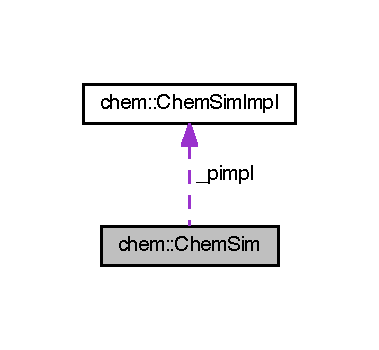
\includegraphics[width=182pt]{classchem_1_1ChemSim__coll__graph}
\end{center}
\end{figure}
\subsection*{Public Member Functions}
\begin{DoxyCompactItemize}
\item 
\hyperlink{classchem_1_1ChemSim_a650a80164d4545c984feae82929ea6d6}{Chem\-Sim} (\hyperlink{classchem_1_1ChemSimImpl}{Chem\-Sim\-Impl} $\ast$csi)
\begin{DoxyCompactList}\small\item\em Constructor. \end{DoxyCompactList}\item 
\hyperlink{classchem_1_1ChemSim_a3913850f42c21b7d047b4516bab90293}{Chem\-Sim} (const \hyperlink{classchem_1_1ChemSim}{Chem\-Sim} \&rhs)
\begin{DoxyCompactList}\small\item\em Copying is not allowed. \end{DoxyCompactList}\item 
\hyperlink{classchem_1_1ChemSim}{Chem\-Sim} \& \hyperlink{classchem_1_1ChemSim_a80f99f736b36adacb3888052f6ab933d}{operator=} (\hyperlink{classchem_1_1ChemSim}{Chem\-Sim} \&rhs)
\begin{DoxyCompactList}\small\item\em Assignment is not allowed. \end{DoxyCompactList}\item 
void \hyperlink{classchem_1_1ChemSim_a691cc53afccbda480a674b7f3014ac72}{initialize} ()
\begin{DoxyCompactList}\small\item\em After all initial reactions have been added via add\-Reaction(...) method, invoke \hyperlink{classchem_1_1ChemSim_a691cc53afccbda480a674b7f3014ac72}{initialize()} prior to invoking \hyperlink{classchem_1_1ChemSim_a1cc6ec051c2f0124bfa327816443b24b}{run()} \end{DoxyCompactList}\item 
void \hyperlink{classchem_1_1ChemSim_a9416fd66c400440bd13779a3060a1ec0}{add\-Reaction} (\hyperlink{classchem_1_1Reaction}{Reaction} $\ast$r)
\begin{DoxyCompactList}\small\item\em Add \hyperlink{classchem_1_1Reaction}{Reaction} $\ast$r to the chemical network which needs to be simulated. \end{DoxyCompactList}\item 
void \hyperlink{classchem_1_1ChemSim_a50f196d75b70e55e0257f20851f8aacf}{remove\-Reaction} (\hyperlink{classchem_1_1Reaction}{Reaction} $\ast$r)
\begin{DoxyCompactList}\small\item\em Remove \hyperlink{classchem_1_1Reaction}{Reaction} $\ast$r from the simulated chemical network. \end{DoxyCompactList}\item 
bool \hyperlink{classchem_1_1ChemSim_a1cc6ec051c2f0124bfa327816443b24b}{run} (int steps)
\begin{DoxyCompactList}\small\item\em Run the chemical dynamics for a specific number of steps. \end{DoxyCompactList}\item 
void \hyperlink{classchem_1_1ChemSim_a95687a56c1c6197aa7513638b8ace4da}{print\-Reactions} () const 
\begin{DoxyCompactList}\small\item\em Mainly used for debugging\-: print chemical reactions in the network at this moment. \end{DoxyCompactList}\end{DoxyCompactItemize}
\subsection*{Private Attributes}
\begin{DoxyCompactItemize}
\item 
\hyperlink{classchem_1_1ChemSimImpl}{Chem\-Sim\-Impl} $\ast$ \hyperlink{classchem_1_1ChemSim_a1e7c8136d1599176ecd517dfd419930a}{\-\_\-pimpl}
\begin{DoxyCompactList}\small\item\em Store a pointer to a specific implementation of stochastic chemical kinetics; no ownership. \end{DoxyCompactList}\end{DoxyCompactItemize}


\subsection{Detailed Description}
\hyperlink{classchem_1_1ChemSim}{Chem\-Sim} is used to manage running a network of chemical reactions. 

\hyperlink{classchem_1_1ChemSim}{Chem\-Sim} implements a Strategy pattern, allowing custom algorithms for running stochastic chemical simulations. After the specific algorithm is chosen and \hyperlink{classchem_1_1ChemSim}{Chem\-Sim} is instantiated, \hyperlink{classchem_1_1ChemSim}{Chem\-Sim} can be used to manage simulations, through such methods as run(steps) etc. Here is an example\-: 
\begin{DoxyCode}
        SpeciesBulk A1("A1",  25);
        SpeciesBulk A2("A2", 25);
        Reaction r1 = { {&A1,&A2}, 1, 1, 100.0 };
        ChemNRMImpl chem_nrm_impl;
        ChemSim chem(&chem_nrm_impl);
        chem.addReaction(&r1);
        chem.initialize();
        chem.printReactions();
        chem.run(100);   
        chem.printReactions();
\end{DoxyCode}
 

Definition at line 37 of file Chem\-Sim.\-h.



\subsection{Constructor \& Destructor Documentation}
\hypertarget{classchem_1_1ChemSim_a650a80164d4545c984feae82929ea6d6}{\index{chem\-::\-Chem\-Sim@{chem\-::\-Chem\-Sim}!Chem\-Sim@{Chem\-Sim}}
\index{Chem\-Sim@{Chem\-Sim}!chem::ChemSim@{chem\-::\-Chem\-Sim}}
\subsubsection[{Chem\-Sim}]{\setlength{\rightskip}{0pt plus 5cm}{\bf chem\-::\-Chem\-Sim\-::\-Chem\-Sim} (
\begin{DoxyParamCaption}
\item[{{\bf Chem\-Sim\-Impl} $\ast$}]{csi}
\end{DoxyParamCaption}
)}}\label{classchem_1_1ChemSim_a650a80164d4545c984feae82929ea6d6}


Constructor. 


\begin{DoxyParams}{Parameters}
{\em \hyperlink{classchem_1_1ChemSimImpl}{Chem\-Sim\-Impl}} & $\ast$csi is a pointer the concrete implementation of stochastic simulation algorithm. \\
\hline
\end{DoxyParams}
\begin{DoxyNote}{Note}
\hyperlink{classchem_1_1ChemSim}{Chem\-Sim} simply stores the csi pointer but does not manage its memory. Make sure that csi is always a valid pointer while \hyperlink{classchem_1_1ChemSim}{Chem\-Sim} is used. 
\end{DoxyNote}


Definition at line 16 of file Chem\-Sim.\-cpp.



References \-\_\-pimpl.

\hypertarget{classchem_1_1ChemSim_a3913850f42c21b7d047b4516bab90293}{\index{chem\-::\-Chem\-Sim@{chem\-::\-Chem\-Sim}!Chem\-Sim@{Chem\-Sim}}
\index{Chem\-Sim@{Chem\-Sim}!chem::ChemSim@{chem\-::\-Chem\-Sim}}
\subsubsection[{Chem\-Sim}]{\setlength{\rightskip}{0pt plus 5cm}{\bf chem\-::\-Chem\-Sim\-::\-Chem\-Sim} (
\begin{DoxyParamCaption}
\item[{const {\bf Chem\-Sim} \&}]{rhs}
\end{DoxyParamCaption}
)}}\label{classchem_1_1ChemSim_a3913850f42c21b7d047b4516bab90293}


Copying is not allowed. 



\subsection{Member Function Documentation}
\hypertarget{classchem_1_1ChemSim_a9416fd66c400440bd13779a3060a1ec0}{\index{chem\-::\-Chem\-Sim@{chem\-::\-Chem\-Sim}!add\-Reaction@{add\-Reaction}}
\index{add\-Reaction@{add\-Reaction}!chem::ChemSim@{chem\-::\-Chem\-Sim}}
\subsubsection[{add\-Reaction}]{\setlength{\rightskip}{0pt plus 5cm}void {\bf chem\-::\-Chem\-Sim\-::add\-Reaction} (
\begin{DoxyParamCaption}
\item[{{\bf Reaction} $\ast$}]{r}
\end{DoxyParamCaption}
)}}\label{classchem_1_1ChemSim_a9416fd66c400440bd13779a3060a1ec0}


Add \hyperlink{classchem_1_1Reaction}{Reaction} $\ast$r to the chemical network which needs to be simulated. 



Definition at line 21 of file Chem\-Sim.\-cpp.



References \-\_\-pimpl, and chem\-::\-Chem\-Sim\-Impl\-::add\-Reaction().



Referenced by main().

\hypertarget{classchem_1_1ChemSim_a691cc53afccbda480a674b7f3014ac72}{\index{chem\-::\-Chem\-Sim@{chem\-::\-Chem\-Sim}!initialize@{initialize}}
\index{initialize@{initialize}!chem::ChemSim@{chem\-::\-Chem\-Sim}}
\subsubsection[{initialize}]{\setlength{\rightskip}{0pt plus 5cm}void {\bf chem\-::\-Chem\-Sim\-::initialize} (
\begin{DoxyParamCaption}
{}
\end{DoxyParamCaption}
)}}\label{classchem_1_1ChemSim_a691cc53afccbda480a674b7f3014ac72}


After all initial reactions have been added via add\-Reaction(...) method, invoke \hyperlink{classchem_1_1ChemSim_a691cc53afccbda480a674b7f3014ac72}{initialize()} prior to invoking \hyperlink{classchem_1_1ChemSim_a1cc6ec051c2f0124bfa327816443b24b}{run()} 



Definition at line 33 of file Chem\-Sim.\-cpp.



References \-\_\-pimpl, and chem\-::\-Chem\-Sim\-Impl\-::initialize().



Referenced by main().

\hypertarget{classchem_1_1ChemSim_a80f99f736b36adacb3888052f6ab933d}{\index{chem\-::\-Chem\-Sim@{chem\-::\-Chem\-Sim}!operator=@{operator=}}
\index{operator=@{operator=}!chem::ChemSim@{chem\-::\-Chem\-Sim}}
\subsubsection[{operator=}]{\setlength{\rightskip}{0pt plus 5cm}{\bf Chem\-Sim}\& chem\-::\-Chem\-Sim\-::operator= (
\begin{DoxyParamCaption}
\item[{{\bf Chem\-Sim} \&}]{rhs}
\end{DoxyParamCaption}
)}}\label{classchem_1_1ChemSim_a80f99f736b36adacb3888052f6ab933d}


Assignment is not allowed. 

\hypertarget{classchem_1_1ChemSim_a95687a56c1c6197aa7513638b8ace4da}{\index{chem\-::\-Chem\-Sim@{chem\-::\-Chem\-Sim}!print\-Reactions@{print\-Reactions}}
\index{print\-Reactions@{print\-Reactions}!chem::ChemSim@{chem\-::\-Chem\-Sim}}
\subsubsection[{print\-Reactions}]{\setlength{\rightskip}{0pt plus 5cm}void {\bf chem\-::\-Chem\-Sim\-::print\-Reactions} (
\begin{DoxyParamCaption}
{}
\end{DoxyParamCaption}
) const}}\label{classchem_1_1ChemSim_a95687a56c1c6197aa7513638b8ace4da}


Mainly used for debugging\-: print chemical reactions in the network at this moment. 



Definition at line 37 of file Chem\-Sim.\-cpp.



References \-\_\-pimpl, and chem\-::\-Chem\-Sim\-Impl\-::print\-Reactions().

\hypertarget{classchem_1_1ChemSim_a50f196d75b70e55e0257f20851f8aacf}{\index{chem\-::\-Chem\-Sim@{chem\-::\-Chem\-Sim}!remove\-Reaction@{remove\-Reaction}}
\index{remove\-Reaction@{remove\-Reaction}!chem::ChemSim@{chem\-::\-Chem\-Sim}}
\subsubsection[{remove\-Reaction}]{\setlength{\rightskip}{0pt plus 5cm}void {\bf chem\-::\-Chem\-Sim\-::remove\-Reaction} (
\begin{DoxyParamCaption}
\item[{{\bf Reaction} $\ast$}]{r}
\end{DoxyParamCaption}
)}}\label{classchem_1_1ChemSim_a50f196d75b70e55e0257f20851f8aacf}


Remove \hyperlink{classchem_1_1Reaction}{Reaction} $\ast$r from the simulated chemical network. 



Definition at line 25 of file Chem\-Sim.\-cpp.



References \-\_\-pimpl, and chem\-::\-Chem\-Sim\-Impl\-::remove\-Reaction().

\hypertarget{classchem_1_1ChemSim_a1cc6ec051c2f0124bfa327816443b24b}{\index{chem\-::\-Chem\-Sim@{chem\-::\-Chem\-Sim}!run@{run}}
\index{run@{run}!chem::ChemSim@{chem\-::\-Chem\-Sim}}
\subsubsection[{run}]{\setlength{\rightskip}{0pt plus 5cm}bool {\bf chem\-::\-Chem\-Sim\-::run} (
\begin{DoxyParamCaption}
\item[{int}]{steps}
\end{DoxyParamCaption}
)}}\label{classchem_1_1ChemSim_a1cc6ec051c2f0124bfa327816443b24b}


Run the chemical dynamics for a specific number of steps. 



Definition at line 29 of file Chem\-Sim.\-cpp.



References \-\_\-pimpl, and chem\-::\-Chem\-Sim\-Impl\-::run().



Referenced by main().



\subsection{Member Data Documentation}
\hypertarget{classchem_1_1ChemSim_a1e7c8136d1599176ecd517dfd419930a}{\index{chem\-::\-Chem\-Sim@{chem\-::\-Chem\-Sim}!\-\_\-pimpl@{\-\_\-pimpl}}
\index{\-\_\-pimpl@{\-\_\-pimpl}!chem::ChemSim@{chem\-::\-Chem\-Sim}}
\subsubsection[{\-\_\-pimpl}]{\setlength{\rightskip}{0pt plus 5cm}{\bf Chem\-Sim\-Impl}$\ast$ {\bf chem\-::\-Chem\-Sim\-::\-\_\-pimpl}\hspace{0.3cm}{\ttfamily  \mbox{[}private\mbox{]}}}}\label{classchem_1_1ChemSim_a1e7c8136d1599176ecd517dfd419930a}


Store a pointer to a specific implementation of stochastic chemical kinetics; no ownership. 



Definition at line 66 of file Chem\-Sim.\-h.



Referenced by add\-Reaction(), Chem\-Sim(), initialize(), print\-Reactions(), remove\-Reaction(), and run().



The documentation for this class was generated from the following files\-:\begin{DoxyCompactItemize}
\item 
Cyto\-Sim/\hyperlink{ChemSim_8h}{Chem\-Sim.\-h}\item 
Cyto\-Sim/\hyperlink{ChemSim_8cpp}{Chem\-Sim.\-cpp}\end{DoxyCompactItemize}

\hypertarget{classchem_1_1ChemSimImpl}{\section{chem\-:\-:Chem\-Sim\-Impl Class Reference}
\label{classchem_1_1ChemSimImpl}\index{chem\-::\-Chem\-Sim\-Impl@{chem\-::\-Chem\-Sim\-Impl}}
}


\hyperlink{classchem_1_1ChemSimImpl}{Chem\-Sim\-Impl} is an abstract base class for algorithms that run stochastic chemical kinetics.  




{\ttfamily \#include $<$Chem\-Sim\-Impl.\-h$>$}



Inheritance diagram for chem\-:\-:Chem\-Sim\-Impl\-:\nopagebreak
\begin{figure}[H]
\begin{center}
\leavevmode
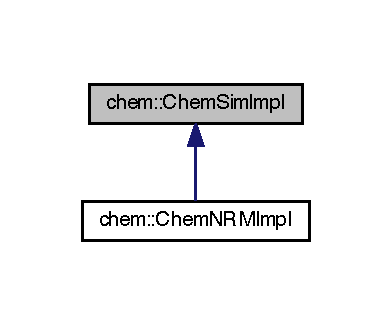
\includegraphics[width=350pt]{classchem_1_1ChemSimImpl__inherit__graph}
\end{center}
\end{figure}
\subsection*{Public Member Functions}
\begin{DoxyCompactItemize}
\item 
virtual \hyperlink{classchem_1_1ChemSimImpl_a54ce9889cf7a09275d2c8257557a5be1}{$\sim$\-Chem\-Sim\-Impl} ()
\item 
virtual void \hyperlink{classchem_1_1ChemSimImpl_a250b43230ac66832bbcecf4f630f2fbc}{initialize} ()=0
\begin{DoxyCompactList}\small\item\em After all initial reactions have been added via add\-Reaction(...) method, invoke \hyperlink{classchem_1_1ChemSimImpl_a250b43230ac66832bbcecf4f630f2fbc}{initialize()} prior to invoking \hyperlink{classchem_1_1ChemSimImpl_a9f051e00a754fdd76d5e2b3a217f3a49}{run()} \end{DoxyCompactList}\item 
virtual void \hyperlink{classchem_1_1ChemSimImpl_a9000e6ec731865360762f483dd7e91cf}{add\-Reaction} (\hyperlink{classchem_1_1Reaction}{Reaction} $\ast$r)=0
\begin{DoxyCompactList}\small\item\em Add \hyperlink{classchem_1_1Reaction}{Reaction} $\ast$r to the chemical network which needs to be simulated. \end{DoxyCompactList}\item 
virtual void \hyperlink{classchem_1_1ChemSimImpl_a00e43cfb099cb26e44d04a715b6cba0a}{remove\-Reaction} (\hyperlink{classchem_1_1Reaction}{Reaction} $\ast$r)=0
\begin{DoxyCompactList}\small\item\em Remove \hyperlink{classchem_1_1Reaction}{Reaction} $\ast$r from the simulated chemical network. \end{DoxyCompactList}\item 
virtual bool \hyperlink{classchem_1_1ChemSimImpl_a9f051e00a754fdd76d5e2b3a217f3a49}{run} (int steps)=0
\begin{DoxyCompactList}\small\item\em Run the chemical dynamics for a specific number of steps. \end{DoxyCompactList}\item 
virtual void \hyperlink{classchem_1_1ChemSimImpl_a24291dac40633358ab6a9f473d6f861d}{print\-Reactions} () const =0
\begin{DoxyCompactList}\small\item\em Mainly used for debugging\-: print chemical reactions in the network at this moment. \end{DoxyCompactList}\end{DoxyCompactItemize}


\subsection{Detailed Description}
\hyperlink{classchem_1_1ChemSimImpl}{Chem\-Sim\-Impl} is an abstract base class for algorithms that run stochastic chemical kinetics. 

Specific stochastic kinetics algorithm classes should inherit from \hyperlink{classchem_1_1ChemSimImpl}{Chem\-Sim\-Impl}. A user will then attach the corresponding algorithm to \hyperlink{classchem_1_1ChemSim}{Chem\-Sim} via the algoritm's base class \hyperlink{classchem_1_1ChemSimImpl}{Chem\-Sim\-Impl}. 

Definition at line 19 of file Chem\-Sim\-Impl.\-h.



\subsection{Constructor \& Destructor Documentation}
\hypertarget{classchem_1_1ChemSimImpl_a54ce9889cf7a09275d2c8257557a5be1}{\index{chem\-::\-Chem\-Sim\-Impl@{chem\-::\-Chem\-Sim\-Impl}!$\sim$\-Chem\-Sim\-Impl@{$\sim$\-Chem\-Sim\-Impl}}
\index{$\sim$\-Chem\-Sim\-Impl@{$\sim$\-Chem\-Sim\-Impl}!chem::ChemSimImpl@{chem\-::\-Chem\-Sim\-Impl}}
\subsubsection[{$\sim$\-Chem\-Sim\-Impl}]{\setlength{\rightskip}{0pt plus 5cm}virtual {\bf chem\-::\-Chem\-Sim\-Impl\-::$\sim$\-Chem\-Sim\-Impl} (
\begin{DoxyParamCaption}
{}
\end{DoxyParamCaption}
)\hspace{0.3cm}{\ttfamily  \mbox{[}inline, virtual\mbox{]}}}}\label{classchem_1_1ChemSimImpl_a54ce9889cf7a09275d2c8257557a5be1}


Definition at line 21 of file Chem\-Sim\-Impl.\-h.



\subsection{Member Function Documentation}
\hypertarget{classchem_1_1ChemSimImpl_a9000e6ec731865360762f483dd7e91cf}{\index{chem\-::\-Chem\-Sim\-Impl@{chem\-::\-Chem\-Sim\-Impl}!add\-Reaction@{add\-Reaction}}
\index{add\-Reaction@{add\-Reaction}!chem::ChemSimImpl@{chem\-::\-Chem\-Sim\-Impl}}
\subsubsection[{add\-Reaction}]{\setlength{\rightskip}{0pt plus 5cm}virtual void {\bf chem\-::\-Chem\-Sim\-Impl\-::add\-Reaction} (
\begin{DoxyParamCaption}
\item[{{\bf Reaction} $\ast$}]{r}
\end{DoxyParamCaption}
)\hspace{0.3cm}{\ttfamily  \mbox{[}pure virtual\mbox{]}}}}\label{classchem_1_1ChemSimImpl_a9000e6ec731865360762f483dd7e91cf}


Add \hyperlink{classchem_1_1Reaction}{Reaction} $\ast$r to the chemical network which needs to be simulated. 



Implemented in \hyperlink{classchem_1_1ChemNRMImpl_a1b325b27b22f443f99fce659ae78aeee}{chem\-::\-Chem\-N\-R\-M\-Impl}, \hyperlink{classchem_1_1ChemGillespieImpl_af013022938adb5f1bd34c7430ad1bfd6}{chem\-::\-Chem\-Gillespie\-Impl}, and \hyperlink{classchem_1_1ChemSimpleGillespieImpl_a0a4146dfe469c85258874f43a2de02a9}{chem\-::\-Chem\-Simple\-Gillespie\-Impl}.



Referenced by chem\-::\-Chem\-Sim\-::add\-Reaction().

\hypertarget{classchem_1_1ChemSimImpl_a250b43230ac66832bbcecf4f630f2fbc}{\index{chem\-::\-Chem\-Sim\-Impl@{chem\-::\-Chem\-Sim\-Impl}!initialize@{initialize}}
\index{initialize@{initialize}!chem::ChemSimImpl@{chem\-::\-Chem\-Sim\-Impl}}
\subsubsection[{initialize}]{\setlength{\rightskip}{0pt plus 5cm}virtual void {\bf chem\-::\-Chem\-Sim\-Impl\-::initialize} (
\begin{DoxyParamCaption}
{}
\end{DoxyParamCaption}
)\hspace{0.3cm}{\ttfamily  \mbox{[}pure virtual\mbox{]}}}}\label{classchem_1_1ChemSimImpl_a250b43230ac66832bbcecf4f630f2fbc}


After all initial reactions have been added via add\-Reaction(...) method, invoke \hyperlink{classchem_1_1ChemSimImpl_a250b43230ac66832bbcecf4f630f2fbc}{initialize()} prior to invoking \hyperlink{classchem_1_1ChemSimImpl_a9f051e00a754fdd76d5e2b3a217f3a49}{run()} 



Implemented in \hyperlink{classchem_1_1ChemNRMImpl_a685ac34bfa4b8226045bd3b8c6cdec95}{chem\-::\-Chem\-N\-R\-M\-Impl}, \hyperlink{classchem_1_1ChemGillespieImpl_a885fd4d5902be9cb7540766e5efc104f}{chem\-::\-Chem\-Gillespie\-Impl}, and \hyperlink{classchem_1_1ChemSimpleGillespieImpl_aa92a28ce1a0217d7224587fcf63f52af}{chem\-::\-Chem\-Simple\-Gillespie\-Impl}.



Referenced by chem\-::\-Chem\-Sim\-::initialize().

\hypertarget{classchem_1_1ChemSimImpl_a24291dac40633358ab6a9f473d6f861d}{\index{chem\-::\-Chem\-Sim\-Impl@{chem\-::\-Chem\-Sim\-Impl}!print\-Reactions@{print\-Reactions}}
\index{print\-Reactions@{print\-Reactions}!chem::ChemSimImpl@{chem\-::\-Chem\-Sim\-Impl}}
\subsubsection[{print\-Reactions}]{\setlength{\rightskip}{0pt plus 5cm}virtual void {\bf chem\-::\-Chem\-Sim\-Impl\-::print\-Reactions} (
\begin{DoxyParamCaption}
{}
\end{DoxyParamCaption}
) const\hspace{0.3cm}{\ttfamily  \mbox{[}pure virtual\mbox{]}}}}\label{classchem_1_1ChemSimImpl_a24291dac40633358ab6a9f473d6f861d}


Mainly used for debugging\-: print chemical reactions in the network at this moment. 



Implemented in \hyperlink{classchem_1_1ChemNRMImpl_a7898a5e226789a39b51f8fb56cc85c1e}{chem\-::\-Chem\-N\-R\-M\-Impl}, \hyperlink{classchem_1_1ChemGillespieImpl_a32d0eac5e52772db6b6b902c08b7df11}{chem\-::\-Chem\-Gillespie\-Impl}, and \hyperlink{classchem_1_1ChemSimpleGillespieImpl_a5ac466ce1f5d1985aa2d7dfd0dcc5162}{chem\-::\-Chem\-Simple\-Gillespie\-Impl}.



Referenced by chem\-::\-Chem\-Sim\-::print\-Reactions().

\hypertarget{classchem_1_1ChemSimImpl_a00e43cfb099cb26e44d04a715b6cba0a}{\index{chem\-::\-Chem\-Sim\-Impl@{chem\-::\-Chem\-Sim\-Impl}!remove\-Reaction@{remove\-Reaction}}
\index{remove\-Reaction@{remove\-Reaction}!chem::ChemSimImpl@{chem\-::\-Chem\-Sim\-Impl}}
\subsubsection[{remove\-Reaction}]{\setlength{\rightskip}{0pt plus 5cm}virtual void {\bf chem\-::\-Chem\-Sim\-Impl\-::remove\-Reaction} (
\begin{DoxyParamCaption}
\item[{{\bf Reaction} $\ast$}]{r}
\end{DoxyParamCaption}
)\hspace{0.3cm}{\ttfamily  \mbox{[}pure virtual\mbox{]}}}}\label{classchem_1_1ChemSimImpl_a00e43cfb099cb26e44d04a715b6cba0a}


Remove \hyperlink{classchem_1_1Reaction}{Reaction} $\ast$r from the simulated chemical network. 



Implemented in \hyperlink{classchem_1_1ChemNRMImpl_ad3a2b84f69c444a55b60d21200537338}{chem\-::\-Chem\-N\-R\-M\-Impl}, \hyperlink{classchem_1_1ChemGillespieImpl_aab4d9fcdd42b90e72542b5b3af103d27}{chem\-::\-Chem\-Gillespie\-Impl}, and \hyperlink{classchem_1_1ChemSimpleGillespieImpl_ad86d7286f61d76db1de522ce333ce7de}{chem\-::\-Chem\-Simple\-Gillespie\-Impl}.



Referenced by chem\-::\-Chem\-Sim\-::remove\-Reaction().

\hypertarget{classchem_1_1ChemSimImpl_a9f051e00a754fdd76d5e2b3a217f3a49}{\index{chem\-::\-Chem\-Sim\-Impl@{chem\-::\-Chem\-Sim\-Impl}!run@{run}}
\index{run@{run}!chem::ChemSimImpl@{chem\-::\-Chem\-Sim\-Impl}}
\subsubsection[{run}]{\setlength{\rightskip}{0pt plus 5cm}virtual bool {\bf chem\-::\-Chem\-Sim\-Impl\-::run} (
\begin{DoxyParamCaption}
\item[{int}]{steps}
\end{DoxyParamCaption}
)\hspace{0.3cm}{\ttfamily  \mbox{[}pure virtual\mbox{]}}}}\label{classchem_1_1ChemSimImpl_a9f051e00a754fdd76d5e2b3a217f3a49}


Run the chemical dynamics for a specific number of steps. 



Implemented in \hyperlink{classchem_1_1ChemNRMImpl_a236b68389599aa9486959377cfc51496}{chem\-::\-Chem\-N\-R\-M\-Impl}, \hyperlink{classchem_1_1ChemGillespieImpl_a5822d60fd10e7c7374150e55c23da075}{chem\-::\-Chem\-Gillespie\-Impl}, and \hyperlink{classchem_1_1ChemSimpleGillespieImpl_a92ac6288318e6bc6882759aac941fa4e}{chem\-::\-Chem\-Simple\-Gillespie\-Impl}.



Referenced by chem\-::\-Chem\-Sim\-::run().



The documentation for this class was generated from the following file\-:\begin{DoxyCompactItemize}
\item 
Cyto\-Sim/\hyperlink{ChemSimImpl_8h}{Chem\-Sim\-Impl.\-h}\end{DoxyCompactItemize}

\input{classchem_1_1ChemSimpleGillespieImpl}
\input{classchem_1_1Compartment}
\input{classchem_1_1CompartmentCubic}
\input{classchem_1_1CompartmentsSimpleGrid}
\hypertarget{classchem_1_1Component}{\section{chem\-:\-:Component Class Reference}
\label{classchem_1_1Component}\index{chem\-::\-Component@{chem\-::\-Component}}
}


{\ttfamily \#include $<$Component.\-h$>$}



Inheritance diagram for chem\-:\-:Component\-:
\nopagebreak
\begin{figure}[H]
\begin{center}
\leavevmode
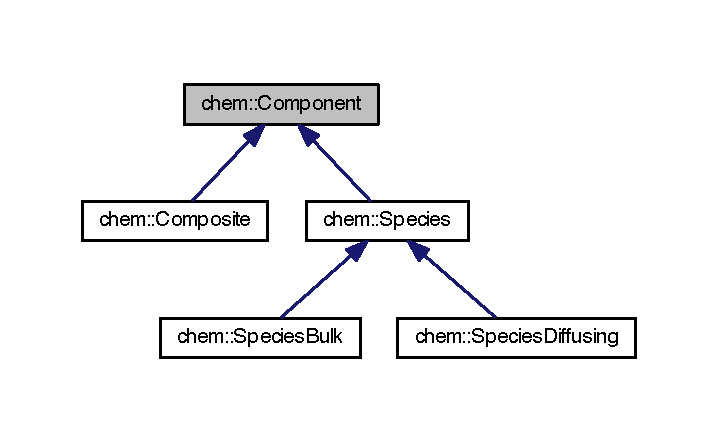
\includegraphics[width=345pt]{classchem_1_1Component__inherit__graph}
\end{center}
\end{figure}


Collaboration diagram for chem\-:\-:Component\-:\nopagebreak
\begin{figure}[H]
\begin{center}
\leavevmode
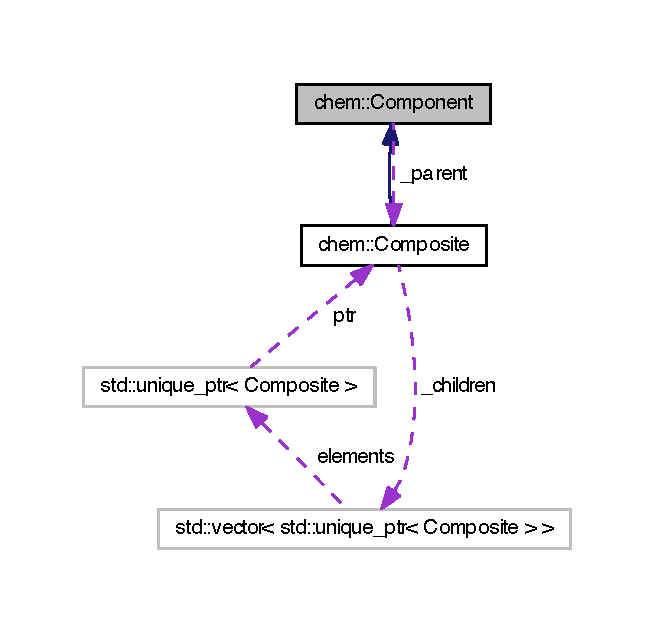
\includegraphics[width=314pt]{classchem_1_1Component__coll__graph}
\end{center}
\end{figure}
\subsection*{Public Member Functions}
\begin{DoxyCompactItemize}
\item 
\hyperlink{classchem_1_1Component_a2c7265280625c13151d52a500bcc3095}{Component} ()
\item 
virtual bool \hyperlink{classchem_1_1Component_ae9efcf2fb203ab7514f81f04d7e4dec2}{apply} (\hyperlink{classchem_1_1Visitor}{Visitor} \&v)
\item 
virtual bool \hyperlink{classchem_1_1Component_ac40e9d75a554324ba1d007a2d5234a38}{apply\-\_\-if} (\hyperlink{classchem_1_1ConditionalVisitor}{Conditional\-Visitor} \&v)
\item 
\hyperlink{classchem_1_1Composite}{Composite} $\ast$ \hyperlink{classchem_1_1Component_a32812270ee52f07ceae2194c56864fd6}{get\-Parent} ()
\item 
void \hyperlink{classchem_1_1Component_a1f4e4d1566f1d3026f1e2a14fa3dffd9}{set\-Parent} (\hyperlink{classchem_1_1Composite}{Composite} $\ast$other)
\item 
bool \hyperlink{classchem_1_1Component_a75cd13a0d884f82fcddd574de33fbfe6}{is\-Root} () const 
\item 
\hyperlink{classchem_1_1Composite}{Composite} $\ast$ \hyperlink{classchem_1_1Component_a7f1166f8fb4c9526cd1794ec3c2714f5}{get\-Root} ()
\item 
virtual size\-\_\-t \hyperlink{classchem_1_1Component_a720ec4ef4aaadfec3e47c31451d28637}{number\-Of\-Children} () const 
\item 
virtual bool \hyperlink{classchem_1_1Component_af2c73f75f937d457a55c1e0120833cb8}{is\-Composite} () const 
\item 
virtual bool \hyperlink{classchem_1_1Component_a3c0f652fe5b6910f07c046fe0190b7b5}{is\-Species\-Container} () const 
\item 
virtual bool \hyperlink{classchem_1_1Component_a8c79ee4335fadfcef56b14a62b742457}{is\-Reactions\-Container} () const 
\item 
virtual \hyperlink{classchem_1_1Component_a9a468e72232a30a69d4432d13ac5ffa9}{$\sim$\-Component} () noexcept
\item 
virtual std\-::string \hyperlink{classchem_1_1Component_a1d5884d373fb44fd950d5fe2b0c34e26}{get\-Full\-Name} () const 
\item 
virtual size\-\_\-t \hyperlink{classchem_1_1Component_a581a3912035ba493a2a24f1516d65ea8}{count\-Species} () const 
\item 
virtual size\-\_\-t \hyperlink{classchem_1_1Component_ab061b8b7d97db554af402ebb9723dc4c}{count\-Reactions} () const 
\item 
virtual void \hyperlink{classchem_1_1Component_a778911b6f9505f1d8a39fc39e093974e}{print\-Self} ()
\end{DoxyCompactItemize}
\subsection*{Private Attributes}
\begin{DoxyCompactItemize}
\item 
\hyperlink{classchem_1_1Composite}{Composite} $\ast$ \hyperlink{classchem_1_1Component_a5da4c5a0d857620fe3e3cf7d8d06ec26}{\-\_\-parent}
\end{DoxyCompactItemize}


\subsection{Detailed Description}


Definition at line 18 of file Component.\-h.



\subsection{Constructor \& Destructor Documentation}
\hypertarget{classchem_1_1Component_a2c7265280625c13151d52a500bcc3095}{\index{chem\-::\-Component@{chem\-::\-Component}!Component@{Component}}
\index{Component@{Component}!chem::Component@{chem\-::\-Component}}
\subsubsection[{Component}]{\setlength{\rightskip}{0pt plus 5cm}{\bf chem\-::\-Component\-::\-Component} (
\begin{DoxyParamCaption}
{}
\end{DoxyParamCaption}
)\hspace{0.3cm}{\ttfamily  \mbox{[}inline\mbox{]}}}}\label{classchem_1_1Component_a2c7265280625c13151d52a500bcc3095}


Definition at line 22 of file Component.\-h.

\hypertarget{classchem_1_1Component_a9a468e72232a30a69d4432d13ac5ffa9}{\index{chem\-::\-Component@{chem\-::\-Component}!$\sim$\-Component@{$\sim$\-Component}}
\index{$\sim$\-Component@{$\sim$\-Component}!chem::Component@{chem\-::\-Component}}
\subsubsection[{$\sim$\-Component}]{\setlength{\rightskip}{0pt plus 5cm}virtual {\bf chem\-::\-Component\-::$\sim$\-Component} (
\begin{DoxyParamCaption}
{}
\end{DoxyParamCaption}
)\hspace{0.3cm}{\ttfamily  \mbox{[}inline, virtual\mbox{]}}}}\label{classchem_1_1Component_a9a468e72232a30a69d4432d13ac5ffa9}


Definition at line 34 of file Component.\-h.



\subsection{Member Function Documentation}
\hypertarget{classchem_1_1Component_ae9efcf2fb203ab7514f81f04d7e4dec2}{\index{chem\-::\-Component@{chem\-::\-Component}!apply@{apply}}
\index{apply@{apply}!chem::Component@{chem\-::\-Component}}
\subsubsection[{apply}]{\setlength{\rightskip}{0pt plus 5cm}bool {\bf chem\-::\-Component\-::apply} (
\begin{DoxyParamCaption}
\item[{{\bf Visitor} \&}]{v}
\end{DoxyParamCaption}
)\hspace{0.3cm}{\ttfamily  \mbox{[}virtual\mbox{]}}}}\label{classchem_1_1Component_ae9efcf2fb203ab7514f81f04d7e4dec2}


Reimplemented in \hyperlink{classchem_1_1Composite_a65464170b82b4531efe620e23e68ea12}{chem\-::\-Composite}.



Definition at line 24 of file Component.\-cpp.



References chem\-::\-Visitor\-::visit().

\hypertarget{classchem_1_1Component_ac40e9d75a554324ba1d007a2d5234a38}{\index{chem\-::\-Component@{chem\-::\-Component}!apply\-\_\-if@{apply\-\_\-if}}
\index{apply\-\_\-if@{apply\-\_\-if}!chem::Component@{chem\-::\-Component}}
\subsubsection[{apply\-\_\-if}]{\setlength{\rightskip}{0pt plus 5cm}bool {\bf chem\-::\-Component\-::apply\-\_\-if} (
\begin{DoxyParamCaption}
\item[{{\bf Conditional\-Visitor} \&}]{v}
\end{DoxyParamCaption}
)\hspace{0.3cm}{\ttfamily  \mbox{[}virtual\mbox{]}}}}\label{classchem_1_1Component_ac40e9d75a554324ba1d007a2d5234a38}


Reimplemented in \hyperlink{classchem_1_1Composite_ac0ef45069901807e72d478ec59736ee4}{chem\-::\-Composite}.



Definition at line 28 of file Component.\-cpp.



References chem\-::\-Conditional\-Visitor\-::visit\-\_\-if().

\hypertarget{classchem_1_1Component_ab061b8b7d97db554af402ebb9723dc4c}{\index{chem\-::\-Component@{chem\-::\-Component}!count\-Reactions@{count\-Reactions}}
\index{count\-Reactions@{count\-Reactions}!chem::Component@{chem\-::\-Component}}
\subsubsection[{count\-Reactions}]{\setlength{\rightskip}{0pt plus 5cm}virtual size\-\_\-t {\bf chem\-::\-Component\-::count\-Reactions} (
\begin{DoxyParamCaption}
{}
\end{DoxyParamCaption}
) const\hspace{0.3cm}{\ttfamily  \mbox{[}inline, virtual\mbox{]}}}}\label{classchem_1_1Component_ab061b8b7d97db554af402ebb9723dc4c}


Reimplemented in \hyperlink{classchem_1_1Composite_a1cba92a649f230eab8e0cecb39632640}{chem\-::\-Composite}.



Definition at line 37 of file Component.\-h.

\hypertarget{classchem_1_1Component_a581a3912035ba493a2a24f1516d65ea8}{\index{chem\-::\-Component@{chem\-::\-Component}!count\-Species@{count\-Species}}
\index{count\-Species@{count\-Species}!chem::Component@{chem\-::\-Component}}
\subsubsection[{count\-Species}]{\setlength{\rightskip}{0pt plus 5cm}virtual size\-\_\-t {\bf chem\-::\-Component\-::count\-Species} (
\begin{DoxyParamCaption}
{}
\end{DoxyParamCaption}
) const\hspace{0.3cm}{\ttfamily  \mbox{[}inline, virtual\mbox{]}}}}\label{classchem_1_1Component_a581a3912035ba493a2a24f1516d65ea8}


Reimplemented in \hyperlink{classchem_1_1Composite_a2c00f5f0be0b7dead8a0a5a53dde1a04}{chem\-::\-Composite}.



Definition at line 36 of file Component.\-h.



Referenced by chem\-::\-Concrete\-Visitor\-::visit(), and chem\-::\-Composite\-Visitor\-::visit().

\hypertarget{classchem_1_1Component_a1d5884d373fb44fd950d5fe2b0c34e26}{\index{chem\-::\-Component@{chem\-::\-Component}!get\-Full\-Name@{get\-Full\-Name}}
\index{get\-Full\-Name@{get\-Full\-Name}!chem::Component@{chem\-::\-Component}}
\subsubsection[{get\-Full\-Name}]{\setlength{\rightskip}{0pt plus 5cm}virtual std\-::string {\bf chem\-::\-Component\-::get\-Full\-Name} (
\begin{DoxyParamCaption}
{}
\end{DoxyParamCaption}
) const\hspace{0.3cm}{\ttfamily  \mbox{[}inline, virtual\mbox{]}}}}\label{classchem_1_1Component_a1d5884d373fb44fd950d5fe2b0c34e26}


Reimplemented in \hyperlink{classchem_1_1CompartmentCubic_aeb15278bbc2c30f7de92ad03e12fbdd5}{chem\-::\-Compartment\-Cubic$<$ N\-D\-I\-M $>$}, \hyperlink{classchem_1_1Compartment_a33a683e6aae89013fce7bde417f49ee1}{chem\-::\-Compartment}, \hyperlink{classchem_1_1Composite_a7781095451c19c48996856153c29bf6b}{chem\-::\-Composite}, and \hyperlink{classchem_1_1CompartmentsSimpleGrid_a9d1006f2fd5ab559bc3ff3f98249ea19}{chem\-::\-Compartments\-Simple\-Grid$<$ N\-D\-I\-M $>$}.



Definition at line 35 of file Component.\-h.



Referenced by chem\-::\-Concrete\-Visitor\-::visit(), chem\-::\-Composite\-Visitor\-::visit(), and chem\-::\-Conditional\-Visitor\-::visit\-\_\-if().

\hypertarget{classchem_1_1Component_a32812270ee52f07ceae2194c56864fd6}{\index{chem\-::\-Component@{chem\-::\-Component}!get\-Parent@{get\-Parent}}
\index{get\-Parent@{get\-Parent}!chem::Component@{chem\-::\-Component}}
\subsubsection[{get\-Parent}]{\setlength{\rightskip}{0pt plus 5cm}{\bf Composite}$\ast$ {\bf chem\-::\-Component\-::get\-Parent} (
\begin{DoxyParamCaption}
{}
\end{DoxyParamCaption}
)\hspace{0.3cm}{\ttfamily  \mbox{[}inline\mbox{]}}}}\label{classchem_1_1Component_a32812270ee52f07ceae2194c56864fd6}


Definition at line 25 of file Component.\-h.



References \-\_\-parent.



Referenced by get\-Root().

\hypertarget{classchem_1_1Component_a7f1166f8fb4c9526cd1794ec3c2714f5}{\index{chem\-::\-Component@{chem\-::\-Component}!get\-Root@{get\-Root}}
\index{get\-Root@{get\-Root}!chem::Component@{chem\-::\-Component}}
\subsubsection[{get\-Root}]{\setlength{\rightskip}{0pt plus 5cm}{\bf Composite} $\ast$ {\bf chem\-::\-Component\-::get\-Root} (
\begin{DoxyParamCaption}
{}
\end{DoxyParamCaption}
)}}\label{classchem_1_1Component_a7f1166f8fb4c9526cd1794ec3c2714f5}


Definition at line 17 of file Component.\-cpp.



References get\-Parent(), get\-Root(), and is\-Root().



Referenced by get\-Root(), chem\-::\-Reaction\-Base\-::get\-Root(), and chem\-::\-Species\-::get\-Root().

\hypertarget{classchem_1_1Component_af2c73f75f937d457a55c1e0120833cb8}{\index{chem\-::\-Component@{chem\-::\-Component}!is\-Composite@{is\-Composite}}
\index{is\-Composite@{is\-Composite}!chem::Component@{chem\-::\-Component}}
\subsubsection[{is\-Composite}]{\setlength{\rightskip}{0pt plus 5cm}virtual bool {\bf chem\-::\-Component\-::is\-Composite} (
\begin{DoxyParamCaption}
{}
\end{DoxyParamCaption}
) const\hspace{0.3cm}{\ttfamily  \mbox{[}inline, virtual\mbox{]}}}}\label{classchem_1_1Component_af2c73f75f937d457a55c1e0120833cb8}


Definition at line 31 of file Component.\-h.

\hypertarget{classchem_1_1Component_a8c79ee4335fadfcef56b14a62b742457}{\index{chem\-::\-Component@{chem\-::\-Component}!is\-Reactions\-Container@{is\-Reactions\-Container}}
\index{is\-Reactions\-Container@{is\-Reactions\-Container}!chem::Component@{chem\-::\-Component}}
\subsubsection[{is\-Reactions\-Container}]{\setlength{\rightskip}{0pt plus 5cm}virtual bool {\bf chem\-::\-Component\-::is\-Reactions\-Container} (
\begin{DoxyParamCaption}
{}
\end{DoxyParamCaption}
) const\hspace{0.3cm}{\ttfamily  \mbox{[}inline, virtual\mbox{]}}}}\label{classchem_1_1Component_a8c79ee4335fadfcef56b14a62b742457}


Reimplemented in \hyperlink{classchem_1_1Compartment_a260d8b2dc70c2834f5702db4743d18ff}{chem\-::\-Compartment}.



Definition at line 33 of file Component.\-h.



Referenced by chem\-::\-Composite\-::count\-Reactions().

\hypertarget{classchem_1_1Component_a75cd13a0d884f82fcddd574de33fbfe6}{\index{chem\-::\-Component@{chem\-::\-Component}!is\-Root@{is\-Root}}
\index{is\-Root@{is\-Root}!chem::Component@{chem\-::\-Component}}
\subsubsection[{is\-Root}]{\setlength{\rightskip}{0pt plus 5cm}bool {\bf chem\-::\-Component\-::is\-Root} (
\begin{DoxyParamCaption}
{}
\end{DoxyParamCaption}
) const\hspace{0.3cm}{\ttfamily  \mbox{[}inline\mbox{]}}}}\label{classchem_1_1Component_a75cd13a0d884f82fcddd574de33fbfe6}


Definition at line 27 of file Component.\-h.



References \-\_\-parent.



Referenced by get\-Root().

\hypertarget{classchem_1_1Component_a3c0f652fe5b6910f07c046fe0190b7b5}{\index{chem\-::\-Component@{chem\-::\-Component}!is\-Species\-Container@{is\-Species\-Container}}
\index{is\-Species\-Container@{is\-Species\-Container}!chem::Component@{chem\-::\-Component}}
\subsubsection[{is\-Species\-Container}]{\setlength{\rightskip}{0pt plus 5cm}virtual bool {\bf chem\-::\-Component\-::is\-Species\-Container} (
\begin{DoxyParamCaption}
{}
\end{DoxyParamCaption}
) const\hspace{0.3cm}{\ttfamily  \mbox{[}inline, virtual\mbox{]}}}}\label{classchem_1_1Component_a3c0f652fe5b6910f07c046fe0190b7b5}


Reimplemented in \hyperlink{classchem_1_1Compartment_a5b31a84f6a592c44ce8235eca96896af}{chem\-::\-Compartment}.



Definition at line 32 of file Component.\-h.



Referenced by chem\-::\-Composite\-::count\-Species().

\hypertarget{classchem_1_1Component_a720ec4ef4aaadfec3e47c31451d28637}{\index{chem\-::\-Component@{chem\-::\-Component}!number\-Of\-Children@{number\-Of\-Children}}
\index{number\-Of\-Children@{number\-Of\-Children}!chem::Component@{chem\-::\-Component}}
\subsubsection[{number\-Of\-Children}]{\setlength{\rightskip}{0pt plus 5cm}virtual size\-\_\-t {\bf chem\-::\-Component\-::number\-Of\-Children} (
\begin{DoxyParamCaption}
{}
\end{DoxyParamCaption}
) const\hspace{0.3cm}{\ttfamily  \mbox{[}inline, virtual\mbox{]}}}}\label{classchem_1_1Component_a720ec4ef4aaadfec3e47c31451d28637}


Reimplemented in \hyperlink{classchem_1_1Composite_a89545dad587539c07acff13398e8ee7a}{chem\-::\-Composite}.



Definition at line 30 of file Component.\-h.

\hypertarget{classchem_1_1Component_a778911b6f9505f1d8a39fc39e093974e}{\index{chem\-::\-Component@{chem\-::\-Component}!print\-Self@{print\-Self}}
\index{print\-Self@{print\-Self}!chem::Component@{chem\-::\-Component}}
\subsubsection[{print\-Self}]{\setlength{\rightskip}{0pt plus 5cm}virtual void {\bf chem\-::\-Component\-::print\-Self} (
\begin{DoxyParamCaption}
{}
\end{DoxyParamCaption}
)\hspace{0.3cm}{\ttfamily  \mbox{[}inline, virtual\mbox{]}}}}\label{classchem_1_1Component_a778911b6f9505f1d8a39fc39e093974e}


Reimplemented in \hyperlink{classchem_1_1CompartmentCubic_a2c7c92befc69c7033c34574f469d5fa8}{chem\-::\-Compartment\-Cubic$<$ N\-D\-I\-M $>$}, \hyperlink{classchem_1_1Compartment_a4b1309d480039e985a7692030e9bca7b}{chem\-::\-Compartment}, and \hyperlink{classchem_1_1CompartmentsSimpleGrid_a5be8454b952a926dd6a7449ff27a3f67}{chem\-::\-Compartments\-Simple\-Grid$<$ N\-D\-I\-M $>$}.



Definition at line 38 of file Component.\-h.

\hypertarget{classchem_1_1Component_a1f4e4d1566f1d3026f1e2a14fa3dffd9}{\index{chem\-::\-Component@{chem\-::\-Component}!set\-Parent@{set\-Parent}}
\index{set\-Parent@{set\-Parent}!chem::Component@{chem\-::\-Component}}
\subsubsection[{set\-Parent}]{\setlength{\rightskip}{0pt plus 5cm}void {\bf chem\-::\-Component\-::set\-Parent} (
\begin{DoxyParamCaption}
\item[{{\bf Composite} $\ast$}]{other}
\end{DoxyParamCaption}
)\hspace{0.3cm}{\ttfamily  \mbox{[}inline\mbox{]}}}}\label{classchem_1_1Component_a1f4e4d1566f1d3026f1e2a14fa3dffd9}


Definition at line 26 of file Component.\-h.



References \-\_\-parent.



\subsection{Member Data Documentation}
\hypertarget{classchem_1_1Component_a5da4c5a0d857620fe3e3cf7d8d06ec26}{\index{chem\-::\-Component@{chem\-::\-Component}!\-\_\-parent@{\-\_\-parent}}
\index{\-\_\-parent@{\-\_\-parent}!chem::Component@{chem\-::\-Component}}
\subsubsection[{\-\_\-parent}]{\setlength{\rightskip}{0pt plus 5cm}{\bf Composite}$\ast$ {\bf chem\-::\-Component\-::\-\_\-parent}\hspace{0.3cm}{\ttfamily  \mbox{[}private\mbox{]}}}}\label{classchem_1_1Component_a5da4c5a0d857620fe3e3cf7d8d06ec26}


Definition at line 20 of file Component.\-h.



Referenced by get\-Parent(), is\-Root(), and set\-Parent().



The documentation for this class was generated from the following files\-:\begin{DoxyCompactItemize}
\item 
Cyto\-Sim/\hyperlink{Component_8h}{Component.\-h}\item 
Cyto\-Sim/\hyperlink{Component_8cpp}{Component.\-cpp}\end{DoxyCompactItemize}

\hypertarget{classchem_1_1Composite}{\section{chem\-:\-:Composite Class Reference}
\label{classchem_1_1Composite}\index{chem\-::\-Composite@{chem\-::\-Composite}}
}


{\ttfamily \#include $<$Composite.\-h$>$}



Inheritance diagram for chem\-:\-:Composite\-:\nopagebreak
\begin{figure}[H]
\begin{center}
\leavevmode
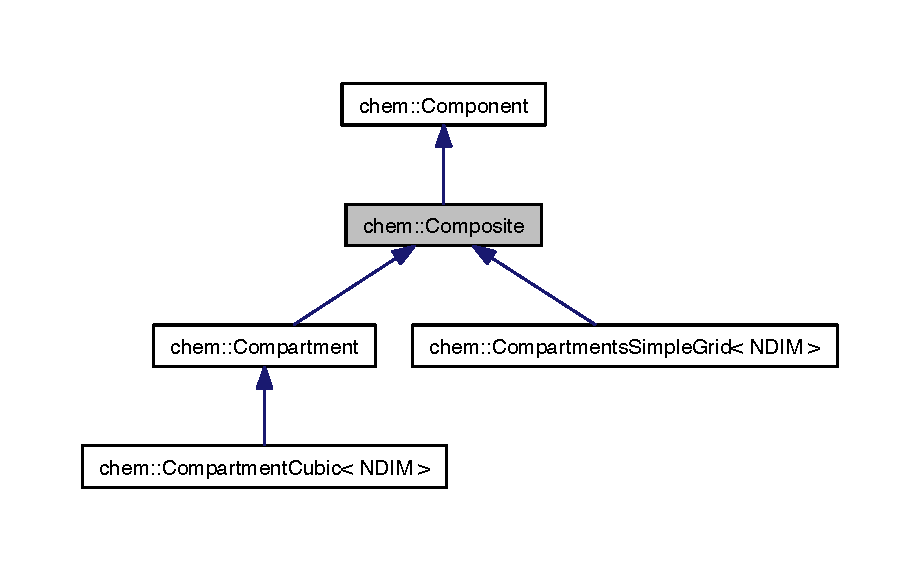
\includegraphics[width=172pt]{classchem_1_1Composite__inherit__graph}
\end{center}
\end{figure}


Collaboration diagram for chem\-:\-:Composite\-:\nopagebreak
\begin{figure}[H]
\begin{center}
\leavevmode
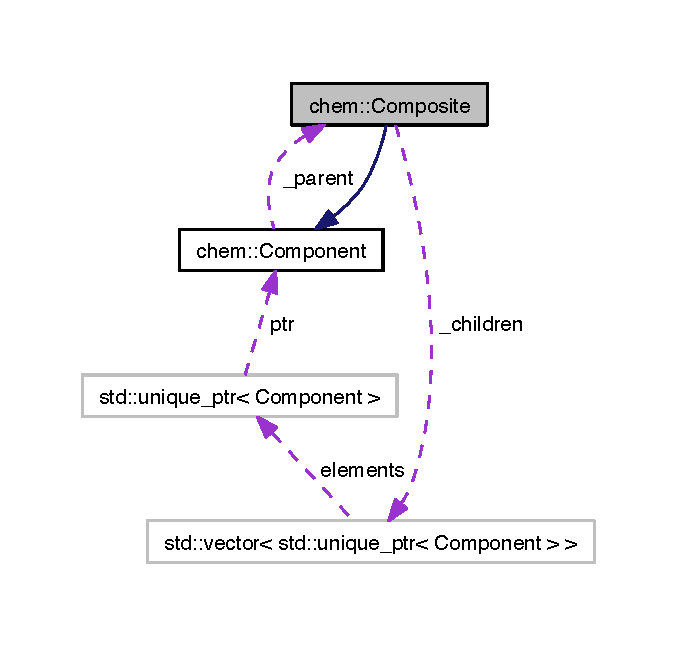
\includegraphics[width=350pt]{classchem_1_1Composite__coll__graph}
\end{center}
\end{figure}
\subsection*{Public Member Functions}
\begin{DoxyCompactItemize}
\item 
\hyperlink{classchem_1_1Composite_ae3444220cf51ab3db2616ea4833c4770}{Composite} ()
\item 
virtual \hyperlink{classchem_1_1Composite_a36a86821952d10911595120d3d26d683}{$\sim$\-Composite} () noexcept
\item 
virtual bool \hyperlink{classchem_1_1Composite_a65464170b82b4531efe620e23e68ea12}{apply} (\hyperlink{classchem_1_1Visitor}{Visitor} \&v)
\item 
virtual bool \hyperlink{classchem_1_1Composite_ac0ef45069901807e72d478ec59736ee4}{apply\-\_\-if} (\hyperlink{classchem_1_1ConditionalVisitor}{Conditional\-Visitor} \&v)
\item 
virtual bool \hyperlink{classchem_1_1Composite_ae4b190f0f14a61d40f68f4a4a51e9192}{is\-Composite} ()
\item 
virtual std\-::string \hyperlink{classchem_1_1Composite_a7781095451c19c48996856153c29bf6b}{get\-Full\-Name} () const 
\item 
virtual void \hyperlink{classchem_1_1Composite_a7f0737d480f68cb2e37eb061a1cfac36}{add\-Child} (std\-::unique\-\_\-ptr$<$ \hyperlink{classchem_1_1Component}{Component} $>$ \&\&child)
\item 
virtual void \hyperlink{classchem_1_1Composite_a1db2418dfbd583f05088fb4695fda677}{remove\-Child} (\hyperlink{classchem_1_1Component}{Component} $\ast$child)
\item 
virtual size\-\_\-t \hyperlink{classchem_1_1Composite_a89545dad587539c07acff13398e8ee7a}{number\-Of\-Children} () const 
\item 
virtual size\-\_\-t \hyperlink{classchem_1_1Composite_a97512e021c76460f0b982d4ff16a91d5}{number\-Of\-Species} () const 
\item 
virtual size\-\_\-t \hyperlink{classchem_1_1Composite_a0089cc7bf318c99339d098018ede34c7}{number\-Of\-Reactions} () const 
\item 
virtual size\-\_\-t \hyperlink{classchem_1_1Composite_a2c00f5f0be0b7dead8a0a5a53dde1a04}{count\-Species} () const 
\item 
virtual size\-\_\-t \hyperlink{classchem_1_1Composite_a1cba92a649f230eab8e0cecb39632640}{count\-Reactions} () const 
\item 
virtual std\-::vector\\*
$<$ std\-::unique\-\_\-ptr$<$ \hyperlink{classchem_1_1Component}{Component} $>$ $>$ \& \hyperlink{classchem_1_1Composite_af4fdad429dc7d8d5014961bbd18c8970}{children} ()
\item 
virtual const std\-::vector\\*
$<$ std\-::unique\-\_\-ptr$<$ \hyperlink{classchem_1_1Component}{Component} $>$ $>$ \& \hyperlink{classchem_1_1Composite_a9c66ed039e22fdafc90627db067fea4b}{children} () const 
\item 
virtual \hyperlink{classchem_1_1Component}{Component} $\ast$ \hyperlink{classchem_1_1Composite_adf797cd6faed6b5f42848c712fd9eb8a}{children} (size\-\_\-t i)
\item 
\hyperlink{classchem_1_1Composite}{Composite} $\ast$ \hyperlink{classchem_1_1Component_a32812270ee52f07ceae2194c56864fd6}{get\-Parent} ()
\item 
void \hyperlink{classchem_1_1Component_a1f4e4d1566f1d3026f1e2a14fa3dffd9}{set\-Parent} (\hyperlink{classchem_1_1Composite}{Composite} $\ast$other)
\item 
bool \hyperlink{classchem_1_1Component_a75cd13a0d884f82fcddd574de33fbfe6}{is\-Root} () const 
\item 
\hyperlink{classchem_1_1Composite}{Composite} $\ast$ \hyperlink{classchem_1_1Component_a7f1166f8fb4c9526cd1794ec3c2714f5}{get\-Root} ()
\item 
virtual bool \hyperlink{classchem_1_1Component_af2c73f75f937d457a55c1e0120833cb8}{is\-Composite} () const 
\item 
virtual bool \hyperlink{classchem_1_1Component_a3c0f652fe5b6910f07c046fe0190b7b5}{is\-Species\-Container} () const 
\item 
virtual bool \hyperlink{classchem_1_1Component_a8c79ee4335fadfcef56b14a62b742457}{is\-Reactions\-Container} () const 
\end{DoxyCompactItemize}
\subsection*{Private Attributes}
\begin{DoxyCompactItemize}
\item 
std\-::vector$<$ std\-::unique\-\_\-ptr\\*
$<$ \hyperlink{classchem_1_1Component}{Component} $>$ $>$ \hyperlink{classchem_1_1Composite_a80fea5cefad1820315fbef6f8d7adf17}{\-\_\-children}
\end{DoxyCompactItemize}


\subsection{Detailed Description}


Definition at line 24 of file Composite.\-h.



\subsection{Constructor \& Destructor Documentation}
\hypertarget{classchem_1_1Composite_ae3444220cf51ab3db2616ea4833c4770}{\index{chem\-::\-Composite@{chem\-::\-Composite}!Composite@{Composite}}
\index{Composite@{Composite}!chem::Composite@{chem\-::\-Composite}}
\subsubsection[{Composite}]{\setlength{\rightskip}{0pt plus 5cm}{\bf chem\-::\-Composite\-::\-Composite} (
\begin{DoxyParamCaption}
{}
\end{DoxyParamCaption}
)\hspace{0.3cm}{\ttfamily  \mbox{[}inline\mbox{]}}}}\label{classchem_1_1Composite_ae3444220cf51ab3db2616ea4833c4770}


Definition at line 29 of file Composite.\-h.

\hypertarget{classchem_1_1Composite_a36a86821952d10911595120d3d26d683}{\index{chem\-::\-Composite@{chem\-::\-Composite}!$\sim$\-Composite@{$\sim$\-Composite}}
\index{$\sim$\-Composite@{$\sim$\-Composite}!chem::Composite@{chem\-::\-Composite}}
\subsubsection[{$\sim$\-Composite}]{\setlength{\rightskip}{0pt plus 5cm}virtual {\bf chem\-::\-Composite\-::$\sim$\-Composite} (
\begin{DoxyParamCaption}
{}
\end{DoxyParamCaption}
)\hspace{0.3cm}{\ttfamily  \mbox{[}inline, virtual\mbox{]}}}}\label{classchem_1_1Composite_a36a86821952d10911595120d3d26d683}


Definition at line 30 of file Composite.\-h.



\subsection{Member Function Documentation}
\hypertarget{classchem_1_1Composite_a7f0737d480f68cb2e37eb061a1cfac36}{\index{chem\-::\-Composite@{chem\-::\-Composite}!add\-Child@{add\-Child}}
\index{add\-Child@{add\-Child}!chem::Composite@{chem\-::\-Composite}}
\subsubsection[{add\-Child}]{\setlength{\rightskip}{0pt plus 5cm}virtual void {\bf chem\-::\-Composite\-::add\-Child} (
\begin{DoxyParamCaption}
\item[{std\-::unique\-\_\-ptr$<$ {\bf Component} $>$ \&\&}]{child}
\end{DoxyParamCaption}
)\hspace{0.3cm}{\ttfamily  \mbox{[}inline, virtual\mbox{]}}}}\label{classchem_1_1Composite_a7f0737d480f68cb2e37eb061a1cfac36}


Definition at line 39 of file Composite.\-h.



References \-\_\-children.

\hypertarget{classchem_1_1Composite_a65464170b82b4531efe620e23e68ea12}{\index{chem\-::\-Composite@{chem\-::\-Composite}!apply@{apply}}
\index{apply@{apply}!chem::Composite@{chem\-::\-Composite}}
\subsubsection[{apply}]{\setlength{\rightskip}{0pt plus 5cm}bool {\bf Composite\-::apply} (
\begin{DoxyParamCaption}
\item[{{\bf Visitor} \&}]{v}
\end{DoxyParamCaption}
)\hspace{0.3cm}{\ttfamily  \mbox{[}virtual\mbox{]}}}}\label{classchem_1_1Composite_a65464170b82b4531efe620e23e68ea12}


Reimplemented from \hyperlink{classchem_1_1Component_ae9efcf2fb203ab7514f81f04d7e4dec2}{chem\-::\-Component}.



Definition at line 15 of file Composite.\-cpp.



References children(), and chem\-::\-Visitor\-::visit().

\hypertarget{classchem_1_1Composite_ac0ef45069901807e72d478ec59736ee4}{\index{chem\-::\-Composite@{chem\-::\-Composite}!apply\-\_\-if@{apply\-\_\-if}}
\index{apply\-\_\-if@{apply\-\_\-if}!chem::Composite@{chem\-::\-Composite}}
\subsubsection[{apply\-\_\-if}]{\setlength{\rightskip}{0pt plus 5cm}bool {\bf Composite\-::apply\-\_\-if} (
\begin{DoxyParamCaption}
\item[{{\bf Conditional\-Visitor} \&}]{v}
\end{DoxyParamCaption}
)\hspace{0.3cm}{\ttfamily  \mbox{[}virtual\mbox{]}}}}\label{classchem_1_1Composite_ac0ef45069901807e72d478ec59736ee4}


Reimplemented from \hyperlink{classchem_1_1Component_ac40e9d75a554324ba1d007a2d5234a38}{chem\-::\-Component}.



Definition at line 27 of file Composite.\-cpp.



References children(), and chem\-::\-Conditional\-Visitor\-::visit\-\_\-if().

\hypertarget{classchem_1_1Composite_af4fdad429dc7d8d5014961bbd18c8970}{\index{chem\-::\-Composite@{chem\-::\-Composite}!children@{children}}
\index{children@{children}!chem::Composite@{chem\-::\-Composite}}
\subsubsection[{children}]{\setlength{\rightskip}{0pt plus 5cm}virtual std\-::vector$<$std\-::unique\-\_\-ptr$<${\bf Component}$>$ $>$\& {\bf chem\-::\-Composite\-::children} (
\begin{DoxyParamCaption}
{}
\end{DoxyParamCaption}
)\hspace{0.3cm}{\ttfamily  \mbox{[}inline, virtual\mbox{]}}}}\label{classchem_1_1Composite_af4fdad429dc7d8d5014961bbd18c8970}


Definition at line 80 of file Composite.\-h.



References \-\_\-children.



Referenced by apply(), apply\-\_\-if(), count\-Reactions(), count\-Species(), and number\-Of\-Children().

\hypertarget{classchem_1_1Composite_a9c66ed039e22fdafc90627db067fea4b}{\index{chem\-::\-Composite@{chem\-::\-Composite}!children@{children}}
\index{children@{children}!chem::Composite@{chem\-::\-Composite}}
\subsubsection[{children}]{\setlength{\rightskip}{0pt plus 5cm}virtual const std\-::vector$<$std\-::unique\-\_\-ptr$<${\bf Component}$>$ $>$\& {\bf chem\-::\-Composite\-::children} (
\begin{DoxyParamCaption}
{}
\end{DoxyParamCaption}
) const\hspace{0.3cm}{\ttfamily  \mbox{[}inline, virtual\mbox{]}}}}\label{classchem_1_1Composite_a9c66ed039e22fdafc90627db067fea4b}


Definition at line 82 of file Composite.\-h.



References \-\_\-children.

\hypertarget{classchem_1_1Composite_adf797cd6faed6b5f42848c712fd9eb8a}{\index{chem\-::\-Composite@{chem\-::\-Composite}!children@{children}}
\index{children@{children}!chem::Composite@{chem\-::\-Composite}}
\subsubsection[{children}]{\setlength{\rightskip}{0pt plus 5cm}virtual {\bf Component}$\ast$ {\bf chem\-::\-Composite\-::children} (
\begin{DoxyParamCaption}
\item[{size\-\_\-t}]{i}
\end{DoxyParamCaption}
)\hspace{0.3cm}{\ttfamily  \mbox{[}inline, virtual\mbox{]}}}}\label{classchem_1_1Composite_adf797cd6faed6b5f42848c712fd9eb8a}


Definition at line 84 of file Composite.\-h.



References \-\_\-children.

\hypertarget{classchem_1_1Composite_a1cba92a649f230eab8e0cecb39632640}{\index{chem\-::\-Composite@{chem\-::\-Composite}!count\-Reactions@{count\-Reactions}}
\index{count\-Reactions@{count\-Reactions}!chem::Composite@{chem\-::\-Composite}}
\subsubsection[{count\-Reactions}]{\setlength{\rightskip}{0pt plus 5cm}virtual size\-\_\-t {\bf chem\-::\-Composite\-::count\-Reactions} (
\begin{DoxyParamCaption}
{}
\end{DoxyParamCaption}
) const\hspace{0.3cm}{\ttfamily  \mbox{[}inline, virtual\mbox{]}}}}\label{classchem_1_1Composite_a1cba92a649f230eab8e0cecb39632640}


Reimplemented from \hyperlink{classchem_1_1Component_ab061b8b7d97db554af402ebb9723dc4c}{chem\-::\-Component}.



Definition at line 71 of file Composite.\-h.



References children(), chem\-::\-Component\-::is\-Reactions\-Container(), and number\-Of\-Reactions().

\hypertarget{classchem_1_1Composite_a2c00f5f0be0b7dead8a0a5a53dde1a04}{\index{chem\-::\-Composite@{chem\-::\-Composite}!count\-Species@{count\-Species}}
\index{count\-Species@{count\-Species}!chem::Composite@{chem\-::\-Composite}}
\subsubsection[{count\-Species}]{\setlength{\rightskip}{0pt plus 5cm}virtual size\-\_\-t {\bf chem\-::\-Composite\-::count\-Species} (
\begin{DoxyParamCaption}
{}
\end{DoxyParamCaption}
) const\hspace{0.3cm}{\ttfamily  \mbox{[}inline, virtual\mbox{]}}}}\label{classchem_1_1Composite_a2c00f5f0be0b7dead8a0a5a53dde1a04}


Reimplemented from \hyperlink{classchem_1_1Component_a581a3912035ba493a2a24f1516d65ea8}{chem\-::\-Component}.



Definition at line 62 of file Composite.\-h.



References children(), chem\-::\-Component\-::is\-Species\-Container(), and number\-Of\-Species().



Referenced by main().

\hypertarget{classchem_1_1Composite_a7781095451c19c48996856153c29bf6b}{\index{chem\-::\-Composite@{chem\-::\-Composite}!get\-Full\-Name@{get\-Full\-Name}}
\index{get\-Full\-Name@{get\-Full\-Name}!chem::Composite@{chem\-::\-Composite}}
\subsubsection[{get\-Full\-Name}]{\setlength{\rightskip}{0pt plus 5cm}virtual std\-::string {\bf chem\-::\-Composite\-::get\-Full\-Name} (
\begin{DoxyParamCaption}
{}
\end{DoxyParamCaption}
) const\hspace{0.3cm}{\ttfamily  \mbox{[}inline, virtual\mbox{]}}}}\label{classchem_1_1Composite_a7781095451c19c48996856153c29bf6b}


Reimplemented from \hyperlink{classchem_1_1Component_a1d5884d373fb44fd950d5fe2b0c34e26}{chem\-::\-Component}.



Reimplemented in \hyperlink{classchem_1_1Compartment_a33a683e6aae89013fce7bde417f49ee1}{chem\-::\-Compartment}.



Definition at line 37 of file Composite.\-h.

\hypertarget{classchem_1_1Component_a32812270ee52f07ceae2194c56864fd6}{\index{chem\-::\-Composite@{chem\-::\-Composite}!get\-Parent@{get\-Parent}}
\index{get\-Parent@{get\-Parent}!chem::Composite@{chem\-::\-Composite}}
\subsubsection[{get\-Parent}]{\setlength{\rightskip}{0pt plus 5cm}{\bf Composite}$\ast$ {\bf chem\-::\-Component\-::get\-Parent} (
\begin{DoxyParamCaption}
{}
\end{DoxyParamCaption}
)\hspace{0.3cm}{\ttfamily  \mbox{[}inline, inherited\mbox{]}}}}\label{classchem_1_1Component_a32812270ee52f07ceae2194c56864fd6}


Definition at line 25 of file Component.\-h.



References chem\-::\-Component\-::\-\_\-parent.



Referenced by chem\-::\-Component\-::get\-Root().

\hypertarget{classchem_1_1Component_a7f1166f8fb4c9526cd1794ec3c2714f5}{\index{chem\-::\-Composite@{chem\-::\-Composite}!get\-Root@{get\-Root}}
\index{get\-Root@{get\-Root}!chem::Composite@{chem\-::\-Composite}}
\subsubsection[{get\-Root}]{\setlength{\rightskip}{0pt plus 5cm}{\bf Composite} $\ast$ {\bf chem\-::\-Component\-::get\-Root} (
\begin{DoxyParamCaption}
{}
\end{DoxyParamCaption}
)\hspace{0.3cm}{\ttfamily  \mbox{[}inherited\mbox{]}}}}\label{classchem_1_1Component_a7f1166f8fb4c9526cd1794ec3c2714f5}


Definition at line 17 of file Component.\-cpp.



References chem\-::\-Component\-::get\-Parent(), chem\-::\-Component\-::get\-Root(), and chem\-::\-Component\-::is\-Root().



Referenced by chem\-::\-Component\-::get\-Root().

\hypertarget{classchem_1_1Component_af2c73f75f937d457a55c1e0120833cb8}{\index{chem\-::\-Composite@{chem\-::\-Composite}!is\-Composite@{is\-Composite}}
\index{is\-Composite@{is\-Composite}!chem::Composite@{chem\-::\-Composite}}
\subsubsection[{is\-Composite}]{\setlength{\rightskip}{0pt plus 5cm}virtual bool {\bf chem\-::\-Component\-::is\-Composite} (
\begin{DoxyParamCaption}
{}
\end{DoxyParamCaption}
) const\hspace{0.3cm}{\ttfamily  \mbox{[}inline, virtual, inherited\mbox{]}}}}\label{classchem_1_1Component_af2c73f75f937d457a55c1e0120833cb8}


Definition at line 31 of file Component.\-h.

\hypertarget{classchem_1_1Composite_ae4b190f0f14a61d40f68f4a4a51e9192}{\index{chem\-::\-Composite@{chem\-::\-Composite}!is\-Composite@{is\-Composite}}
\index{is\-Composite@{is\-Composite}!chem::Composite@{chem\-::\-Composite}}
\subsubsection[{is\-Composite}]{\setlength{\rightskip}{0pt plus 5cm}virtual bool {\bf chem\-::\-Composite\-::is\-Composite} (
\begin{DoxyParamCaption}
{}
\end{DoxyParamCaption}
)\hspace{0.3cm}{\ttfamily  \mbox{[}inline, virtual\mbox{]}}}}\label{classchem_1_1Composite_ae4b190f0f14a61d40f68f4a4a51e9192}


Definition at line 35 of file Composite.\-h.

\hypertarget{classchem_1_1Component_a8c79ee4335fadfcef56b14a62b742457}{\index{chem\-::\-Composite@{chem\-::\-Composite}!is\-Reactions\-Container@{is\-Reactions\-Container}}
\index{is\-Reactions\-Container@{is\-Reactions\-Container}!chem::Composite@{chem\-::\-Composite}}
\subsubsection[{is\-Reactions\-Container}]{\setlength{\rightskip}{0pt plus 5cm}virtual bool {\bf chem\-::\-Component\-::is\-Reactions\-Container} (
\begin{DoxyParamCaption}
{}
\end{DoxyParamCaption}
) const\hspace{0.3cm}{\ttfamily  \mbox{[}inline, virtual, inherited\mbox{]}}}}\label{classchem_1_1Component_a8c79ee4335fadfcef56b14a62b742457}


Reimplemented in \hyperlink{classchem_1_1Compartment_a260d8b2dc70c2834f5702db4743d18ff}{chem\-::\-Compartment}.



Definition at line 33 of file Component.\-h.



Referenced by count\-Reactions().

\hypertarget{classchem_1_1Component_a75cd13a0d884f82fcddd574de33fbfe6}{\index{chem\-::\-Composite@{chem\-::\-Composite}!is\-Root@{is\-Root}}
\index{is\-Root@{is\-Root}!chem::Composite@{chem\-::\-Composite}}
\subsubsection[{is\-Root}]{\setlength{\rightskip}{0pt plus 5cm}bool {\bf chem\-::\-Component\-::is\-Root} (
\begin{DoxyParamCaption}
{}
\end{DoxyParamCaption}
) const\hspace{0.3cm}{\ttfamily  \mbox{[}inline, inherited\mbox{]}}}}\label{classchem_1_1Component_a75cd13a0d884f82fcddd574de33fbfe6}


Definition at line 27 of file Component.\-h.



References chem\-::\-Component\-::\-\_\-parent.



Referenced by chem\-::\-Component\-::get\-Root().

\hypertarget{classchem_1_1Component_a3c0f652fe5b6910f07c046fe0190b7b5}{\index{chem\-::\-Composite@{chem\-::\-Composite}!is\-Species\-Container@{is\-Species\-Container}}
\index{is\-Species\-Container@{is\-Species\-Container}!chem::Composite@{chem\-::\-Composite}}
\subsubsection[{is\-Species\-Container}]{\setlength{\rightskip}{0pt plus 5cm}virtual bool {\bf chem\-::\-Component\-::is\-Species\-Container} (
\begin{DoxyParamCaption}
{}
\end{DoxyParamCaption}
) const\hspace{0.3cm}{\ttfamily  \mbox{[}inline, virtual, inherited\mbox{]}}}}\label{classchem_1_1Component_a3c0f652fe5b6910f07c046fe0190b7b5}


Reimplemented in \hyperlink{classchem_1_1Compartment_a5b31a84f6a592c44ce8235eca96896af}{chem\-::\-Compartment}.



Definition at line 32 of file Component.\-h.



Referenced by count\-Species().

\hypertarget{classchem_1_1Composite_a89545dad587539c07acff13398e8ee7a}{\index{chem\-::\-Composite@{chem\-::\-Composite}!number\-Of\-Children@{number\-Of\-Children}}
\index{number\-Of\-Children@{number\-Of\-Children}!chem::Composite@{chem\-::\-Composite}}
\subsubsection[{number\-Of\-Children}]{\setlength{\rightskip}{0pt plus 5cm}virtual size\-\_\-t {\bf chem\-::\-Composite\-::number\-Of\-Children} (
\begin{DoxyParamCaption}
{}
\end{DoxyParamCaption}
) const\hspace{0.3cm}{\ttfamily  \mbox{[}inline, virtual\mbox{]}}}}\label{classchem_1_1Composite_a89545dad587539c07acff13398e8ee7a}


Reimplemented from \hyperlink{classchem_1_1Component_a720ec4ef4aaadfec3e47c31451d28637}{chem\-::\-Component}.



Definition at line 56 of file Composite.\-h.



References children().

\hypertarget{classchem_1_1Composite_a0089cc7bf318c99339d098018ede34c7}{\index{chem\-::\-Composite@{chem\-::\-Composite}!number\-Of\-Reactions@{number\-Of\-Reactions}}
\index{number\-Of\-Reactions@{number\-Of\-Reactions}!chem::Composite@{chem\-::\-Composite}}
\subsubsection[{number\-Of\-Reactions}]{\setlength{\rightskip}{0pt plus 5cm}virtual size\-\_\-t {\bf chem\-::\-Composite\-::number\-Of\-Reactions} (
\begin{DoxyParamCaption}
{}
\end{DoxyParamCaption}
) const\hspace{0.3cm}{\ttfamily  \mbox{[}inline, virtual\mbox{]}}}}\label{classchem_1_1Composite_a0089cc7bf318c99339d098018ede34c7}


Reimplemented in \hyperlink{classchem_1_1Compartment_add01255fb00b50c58bd65edc66c25d7a}{chem\-::\-Compartment}.



Definition at line 60 of file Composite.\-h.



Referenced by count\-Reactions().

\hypertarget{classchem_1_1Composite_a97512e021c76460f0b982d4ff16a91d5}{\index{chem\-::\-Composite@{chem\-::\-Composite}!number\-Of\-Species@{number\-Of\-Species}}
\index{number\-Of\-Species@{number\-Of\-Species}!chem::Composite@{chem\-::\-Composite}}
\subsubsection[{number\-Of\-Species}]{\setlength{\rightskip}{0pt plus 5cm}virtual size\-\_\-t {\bf chem\-::\-Composite\-::number\-Of\-Species} (
\begin{DoxyParamCaption}
{}
\end{DoxyParamCaption}
) const\hspace{0.3cm}{\ttfamily  \mbox{[}inline, virtual\mbox{]}}}}\label{classchem_1_1Composite_a97512e021c76460f0b982d4ff16a91d5}


Reimplemented in \hyperlink{classchem_1_1Compartment_a8c53c911ee4474486eb479d869b83a23}{chem\-::\-Compartment}.



Definition at line 58 of file Composite.\-h.



Referenced by count\-Species().

\hypertarget{classchem_1_1Composite_a1db2418dfbd583f05088fb4695fda677}{\index{chem\-::\-Composite@{chem\-::\-Composite}!remove\-Child@{remove\-Child}}
\index{remove\-Child@{remove\-Child}!chem::Composite@{chem\-::\-Composite}}
\subsubsection[{remove\-Child}]{\setlength{\rightskip}{0pt plus 5cm}virtual void {\bf chem\-::\-Composite\-::remove\-Child} (
\begin{DoxyParamCaption}
\item[{{\bf Component} $\ast$}]{child}
\end{DoxyParamCaption}
)\hspace{0.3cm}{\ttfamily  \mbox{[}inline, virtual\mbox{]}}}}\label{classchem_1_1Composite_a1db2418dfbd583f05088fb4695fda677}


Definition at line 44 of file Composite.\-h.



References \-\_\-children.

\hypertarget{classchem_1_1Component_a1f4e4d1566f1d3026f1e2a14fa3dffd9}{\index{chem\-::\-Composite@{chem\-::\-Composite}!set\-Parent@{set\-Parent}}
\index{set\-Parent@{set\-Parent}!chem::Composite@{chem\-::\-Composite}}
\subsubsection[{set\-Parent}]{\setlength{\rightskip}{0pt plus 5cm}void {\bf chem\-::\-Component\-::set\-Parent} (
\begin{DoxyParamCaption}
\item[{{\bf Composite} $\ast$}]{other}
\end{DoxyParamCaption}
)\hspace{0.3cm}{\ttfamily  \mbox{[}inline, inherited\mbox{]}}}}\label{classchem_1_1Component_a1f4e4d1566f1d3026f1e2a14fa3dffd9}


Definition at line 26 of file Component.\-h.



References chem\-::\-Component\-::\-\_\-parent.



Referenced by chem\-::\-Compartment\-::add\-Reaction(), chem\-::\-Compartment\-::add\-Reaction\-Unique(), chem\-::\-Compartment\-::add\-Species(), and chem\-::\-Compartment\-::add\-Species\-Unique().



\subsection{Member Data Documentation}
\hypertarget{classchem_1_1Composite_a80fea5cefad1820315fbef6f8d7adf17}{\index{chem\-::\-Composite@{chem\-::\-Composite}!\-\_\-children@{\-\_\-children}}
\index{\-\_\-children@{\-\_\-children}!chem::Composite@{chem\-::\-Composite}}
\subsubsection[{\-\_\-children}]{\setlength{\rightskip}{0pt plus 5cm}std\-::vector$<$std\-::unique\-\_\-ptr$<${\bf Component}$>$ $>$ {\bf chem\-::\-Composite\-::\-\_\-children}\hspace{0.3cm}{\ttfamily  \mbox{[}private\mbox{]}}}}\label{classchem_1_1Composite_a80fea5cefad1820315fbef6f8d7adf17}


Definition at line 26 of file Composite.\-h.



Referenced by add\-Child(), children(), and remove\-Child().



The documentation for this class was generated from the following files\-:\begin{DoxyCompactItemize}
\item 
Cyto\-Sim/\hyperlink{Composite_8h}{Composite.\-h}\item 
Cyto\-Sim/\hyperlink{Composite_8cpp}{Composite.\-cpp}\end{DoxyCompactItemize}

\hypertarget{classchem_1_1CompositeVisitor}{\section{chem\-:\-:Composite\-Visitor Class Reference}
\label{classchem_1_1CompositeVisitor}\index{chem\-::\-Composite\-Visitor@{chem\-::\-Composite\-Visitor}}
}


{\ttfamily \#include $<$Visitor\-Concrete.\-h$>$}



Inheritance diagram for chem\-:\-:Composite\-Visitor\-:
\nopagebreak
\begin{figure}[H]
\begin{center}
\leavevmode
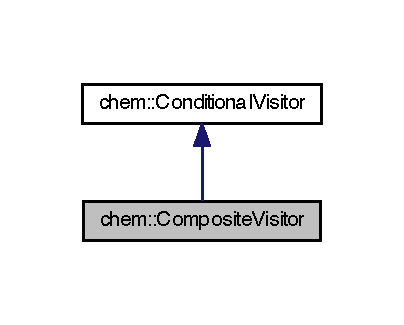
\includegraphics[width=200pt]{classchem_1_1CompositeVisitor__inherit__graph}
\end{center}
\end{figure}


Collaboration diagram for chem\-:\-:Composite\-Visitor\-:
\nopagebreak
\begin{figure}[H]
\begin{center}
\leavevmode
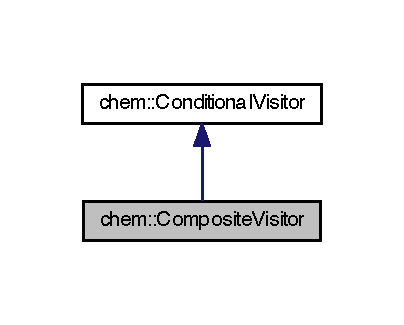
\includegraphics[width=200pt]{classchem_1_1CompositeVisitor__coll__graph}
\end{center}
\end{figure}
\subsection*{Public Member Functions}
\begin{DoxyCompactItemize}
\item 
bool \hyperlink{classchem_1_1Visitor_a710015ef735e109c812edbb653d6d598}{visit} (\hyperlink{classchem_1_1Component}{Component} $\ast$c)
\begin{DoxyCompactList}\small\item\em When this visitor, $\ast$v, is propagated through the \hyperlink{classchem_1_1Composite}{Composite} hieararchy, at each \hyperlink{classchem_1_1Component}{Component} node pointer $\ast$c, the following method is called\-: v-\/$>$visit(c). \end{DoxyCompactList}\item 
bool \hyperlink{classchem_1_1Visitor_ad02a683bb0cf97d9df381c3efeb90a06}{visit\-\_\-if} (\hyperlink{classchem_1_1Component}{Component} $\ast$c)
\begin{DoxyCompactList}\small\item\em When this conditional visitor, $\ast$cv, is propagated through the \hyperlink{classchem_1_1Composite}{Composite} hieararchy, at each \hyperlink{classchem_1_1Component}{Component} node pointer $\ast$c, the following method is called\-: v-\/$>$visit(c), if v-\/$>$pred(c) returns true. \end{DoxyCompactList}\end{DoxyCompactItemize}
\subsection*{Protected Member Functions}
\begin{DoxyCompactItemize}
\item 
virtual bool \hyperlink{classchem_1_1CompositeVisitor_ac3104d5ec0d0628bbcc72f17f69b0396}{visit\-Impl} (\hyperlink{classchem_1_1Component}{Component} $\ast$c) override
\begin{DoxyCompactList}\small\item\em When this visitor, $\ast$cv, is propagated through the \hyperlink{classchem_1_1Composite}{Composite} hieararchy, at each \hyperlink{classchem_1_1Component}{Component} node pointer $\ast$c, the following method is called\-: cv-\/$>$visit(c). \end{DoxyCompactList}\item 
virtual bool \hyperlink{classchem_1_1CompositeVisitor_a157e17e7a6b7ed91b47d59aea1cc1268}{pred\-Impl} (\hyperlink{classchem_1_1Component}{Component} $\ast$c) override
\begin{DoxyCompactList}\small\item\em Return true if the \hyperlink{classchem_1_1Component}{Component} $\ast$c satisfies the desired predicate. \end{DoxyCompactList}\end{DoxyCompactItemize}


\subsection{Detailed Description}


Definition at line 50 of file Visitor\-Concrete.\-h.



\subsection{Member Function Documentation}
\hypertarget{classchem_1_1CompositeVisitor_a157e17e7a6b7ed91b47d59aea1cc1268}{\index{chem\-::\-Composite\-Visitor@{chem\-::\-Composite\-Visitor}!pred\-Impl@{pred\-Impl}}
\index{pred\-Impl@{pred\-Impl}!chem::CompositeVisitor@{chem\-::\-Composite\-Visitor}}
\subsubsection[{pred\-Impl}]{\setlength{\rightskip}{0pt plus 5cm}virtual bool {\bf chem\-::\-Composite\-Visitor\-::pred\-Impl} (
\begin{DoxyParamCaption}
\item[{{\bf Component} $\ast$}]{c}
\end{DoxyParamCaption}
)\hspace{0.3cm}{\ttfamily  \mbox{[}inline, override, protected, virtual\mbox{]}}}}\label{classchem_1_1CompositeVisitor_a157e17e7a6b7ed91b47d59aea1cc1268}


Return true if the \hyperlink{classchem_1_1Component}{Component} $\ast$c satisfies the desired predicate. 



Implements \hyperlink{classchem_1_1Visitor_a8f11a43266d18d1396236d0c5f3a8ad6}{chem\-::\-Visitor}.



Definition at line 57 of file Visitor\-Concrete.\-h.

\hypertarget{classchem_1_1Visitor_a710015ef735e109c812edbb653d6d598}{\index{chem\-::\-Composite\-Visitor@{chem\-::\-Composite\-Visitor}!visit@{visit}}
\index{visit@{visit}!chem::CompositeVisitor@{chem\-::\-Composite\-Visitor}}
\subsubsection[{visit}]{\setlength{\rightskip}{0pt plus 5cm}bool {\bf chem\-::\-Visitor\-::visit} (
\begin{DoxyParamCaption}
\item[{{\bf Component} $\ast$}]{c}
\end{DoxyParamCaption}
)\hspace{0.3cm}{\ttfamily  \mbox{[}inline, inherited\mbox{]}}}}\label{classchem_1_1Visitor_a710015ef735e109c812edbb653d6d598}


When this visitor, $\ast$v, is propagated through the \hyperlink{classchem_1_1Composite}{Composite} hieararchy, at each \hyperlink{classchem_1_1Component}{Component} node pointer $\ast$c, the following method is called\-: v-\/$>$visit(c). 

If a false value is returned from this function called, then the further propagation of the tree is terminated. 

Definition at line 31 of file Visitor.\-h.



References chem\-::\-Visitor\-::visit\-Impl().



Referenced by chem\-::\-Component\-::apply(), and chem\-::\-Composite\-::apply().

\hypertarget{classchem_1_1Visitor_ad02a683bb0cf97d9df381c3efeb90a06}{\index{chem\-::\-Composite\-Visitor@{chem\-::\-Composite\-Visitor}!visit\-\_\-if@{visit\-\_\-if}}
\index{visit\-\_\-if@{visit\-\_\-if}!chem::CompositeVisitor@{chem\-::\-Composite\-Visitor}}
\subsubsection[{visit\-\_\-if}]{\setlength{\rightskip}{0pt plus 5cm}bool {\bf chem\-::\-Visitor\-::visit\-\_\-if} (
\begin{DoxyParamCaption}
\item[{{\bf Component} $\ast$}]{c}
\end{DoxyParamCaption}
)\hspace{0.3cm}{\ttfamily  \mbox{[}inline, inherited\mbox{]}}}}\label{classchem_1_1Visitor_ad02a683bb0cf97d9df381c3efeb90a06}


When this conditional visitor, $\ast$cv, is propagated through the \hyperlink{classchem_1_1Composite}{Composite} hieararchy, at each \hyperlink{classchem_1_1Component}{Component} node pointer $\ast$c, the following method is called\-: v-\/$>$visit(c), if v-\/$>$pred(c) returns true. 

If v-\/$>$visit(c) returns a false value, then the further propagation of the tree is terminated. 

Definition at line 36 of file Visitor.\-h.



References chem\-::\-Visitor\-::pred\-Impl(), and chem\-::\-Visitor\-::visit\-Impl().



Referenced by chem\-::\-Component\-::apply\-\_\-if(), and chem\-::\-Composite\-::apply\-\_\-if().

\hypertarget{classchem_1_1CompositeVisitor_ac3104d5ec0d0628bbcc72f17f69b0396}{\index{chem\-::\-Composite\-Visitor@{chem\-::\-Composite\-Visitor}!visit\-Impl@{visit\-Impl}}
\index{visit\-Impl@{visit\-Impl}!chem::CompositeVisitor@{chem\-::\-Composite\-Visitor}}
\subsubsection[{visit\-Impl}]{\setlength{\rightskip}{0pt plus 5cm}virtual bool {\bf chem\-::\-Composite\-Visitor\-::visit\-Impl} (
\begin{DoxyParamCaption}
\item[{{\bf Component} $\ast$}]{c}
\end{DoxyParamCaption}
)\hspace{0.3cm}{\ttfamily  \mbox{[}inline, override, protected, virtual\mbox{]}}}}\label{classchem_1_1CompositeVisitor_ac3104d5ec0d0628bbcc72f17f69b0396}


When this visitor, $\ast$cv, is propagated through the \hyperlink{classchem_1_1Composite}{Composite} hieararchy, at each \hyperlink{classchem_1_1Component}{Component} node pointer $\ast$c, the following method is called\-: cv-\/$>$visit(c). 

If a false value is returned from this function called, then the further propagation of the tree is terminated. 

Implements \hyperlink{classchem_1_1Visitor_ae058e8ac35f22b03d23ae443d12c71ea}{chem\-::\-Visitor}.



Definition at line 52 of file Visitor\-Concrete.\-h.



References chem\-::\-Component\-::count\-Species(), and chem\-::\-Component\-::get\-Full\-Name().



The documentation for this class was generated from the following file\-:\begin{DoxyCompactItemize}
\item 
Cyto\-Sim/\hyperlink{VisitorConcrete_8h}{Visitor\-Concrete.\-h}\end{DoxyCompactItemize}

\hypertarget{classchem_1_1ConcreteVisitor}{\section{chem\-:\-:Concrete\-Visitor Class Reference}
\label{classchem_1_1ConcreteVisitor}\index{chem\-::\-Concrete\-Visitor@{chem\-::\-Concrete\-Visitor}}
}


{\ttfamily \#include $<$Visitor\-Concrete.\-h$>$}



Inheritance diagram for chem\-:\-:Concrete\-Visitor\-:\nopagebreak
\begin{figure}[H]
\begin{center}
\leavevmode
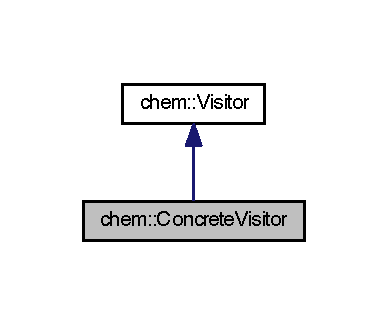
\includegraphics[width=186pt]{classchem_1_1ConcreteVisitor__inherit__graph}
\end{center}
\end{figure}


Collaboration diagram for chem\-:\-:Concrete\-Visitor\-:\nopagebreak
\begin{figure}[H]
\begin{center}
\leavevmode
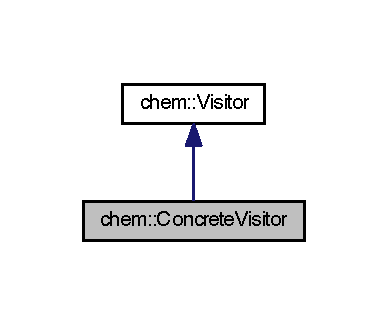
\includegraphics[width=186pt]{classchem_1_1ConcreteVisitor__coll__graph}
\end{center}
\end{figure}
\subsection*{Public Member Functions}
\begin{DoxyCompactItemize}
\item 
virtual bool \hyperlink{classchem_1_1ConcreteVisitor_abb5892cdcf90fef25aafafaf81baa697}{visit} (\hyperlink{classchem_1_1Component}{Component} $\ast$c)
\end{DoxyCompactItemize}


\subsection{Detailed Description}


Definition at line 19 of file Visitor\-Concrete.\-h.



\subsection{Member Function Documentation}
\hypertarget{classchem_1_1ConcreteVisitor_abb5892cdcf90fef25aafafaf81baa697}{\index{chem\-::\-Concrete\-Visitor@{chem\-::\-Concrete\-Visitor}!visit@{visit}}
\index{visit@{visit}!chem::ConcreteVisitor@{chem\-::\-Concrete\-Visitor}}
\subsubsection[{visit}]{\setlength{\rightskip}{0pt plus 5cm}virtual bool {\bf chem\-::\-Concrete\-Visitor\-::visit} (
\begin{DoxyParamCaption}
\item[{{\bf Component} $\ast$}]{c}
\end{DoxyParamCaption}
)\hspace{0.3cm}{\ttfamily  \mbox{[}inline, virtual\mbox{]}}}}\label{classchem_1_1ConcreteVisitor_abb5892cdcf90fef25aafafaf81baa697}


Implements \hyperlink{classchem_1_1Visitor_a3a148d3144ed2ef25972509a6a594d1a}{chem\-::\-Visitor}.



Definition at line 21 of file Visitor\-Concrete.\-h.



References chem\-::\-Component\-::count\-Species(), and chem\-::\-Component\-::get\-Full\-Name().



The documentation for this class was generated from the following file\-:\begin{DoxyCompactItemize}
\item 
Cyto\-Sim/\hyperlink{VisitorConcrete_8h}{Visitor\-Concrete.\-h}\end{DoxyCompactItemize}

\hypertarget{classchem_1_1ConditionalVisitor}{\section{chem\-:\-:Conditional\-Visitor Class Reference}
\label{classchem_1_1ConditionalVisitor}\index{chem\-::\-Conditional\-Visitor@{chem\-::\-Conditional\-Visitor}}
}


{\ttfamily \#include $<$Visitor.\-h$>$}



Inheritance diagram for chem\-:\-:Conditional\-Visitor\-:\nopagebreak
\begin{figure}[H]
\begin{center}
\leavevmode
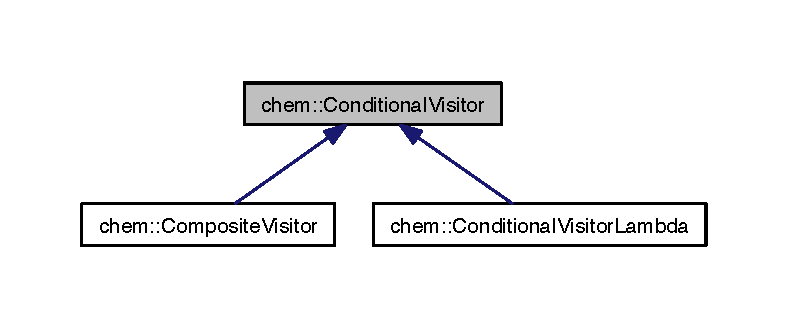
\includegraphics[width=194pt]{classchem_1_1ConditionalVisitor__inherit__graph}
\end{center}
\end{figure}
\subsection*{Public Member Functions}
\begin{DoxyCompactItemize}
\item 
virtual bool \hyperlink{classchem_1_1ConditionalVisitor_ac5eca1778f8647f7dc85a00489c3d938}{visit\-\_\-if} (\hyperlink{classchem_1_1Component}{Component} $\ast$c)
\item 
virtual bool \hyperlink{classchem_1_1ConditionalVisitor_aff08b8bc4b5c193e1fe60f06cca318b1}{visit} (\hyperlink{classchem_1_1Component}{Component} $\ast$c)=0
\item 
virtual bool \hyperlink{classchem_1_1ConditionalVisitor_ac35925bee54467373d1f44cccec75aa5}{pred} (\hyperlink{classchem_1_1Component}{Component} $\ast$c)=0
\item 
virtual \hyperlink{classchem_1_1ConditionalVisitor_ad4f7c23e000b587469b74455e5c1a8b7}{$\sim$\-Conditional\-Visitor} ()
\end{DoxyCompactItemize}


\subsection{Detailed Description}


Definition at line 23 of file Visitor.\-h.



\subsection{Constructor \& Destructor Documentation}
\hypertarget{classchem_1_1ConditionalVisitor_ad4f7c23e000b587469b74455e5c1a8b7}{\index{chem\-::\-Conditional\-Visitor@{chem\-::\-Conditional\-Visitor}!$\sim$\-Conditional\-Visitor@{$\sim$\-Conditional\-Visitor}}
\index{$\sim$\-Conditional\-Visitor@{$\sim$\-Conditional\-Visitor}!chem::ConditionalVisitor@{chem\-::\-Conditional\-Visitor}}
\subsubsection[{$\sim$\-Conditional\-Visitor}]{\setlength{\rightskip}{0pt plus 5cm}virtual {\bf chem\-::\-Conditional\-Visitor\-::$\sim$\-Conditional\-Visitor} (
\begin{DoxyParamCaption}
{}
\end{DoxyParamCaption}
)\hspace{0.3cm}{\ttfamily  \mbox{[}inline, virtual\mbox{]}}}}\label{classchem_1_1ConditionalVisitor_ad4f7c23e000b587469b74455e5c1a8b7}


Definition at line 37 of file Visitor.\-h.



\subsection{Member Function Documentation}
\hypertarget{classchem_1_1ConditionalVisitor_ac35925bee54467373d1f44cccec75aa5}{\index{chem\-::\-Conditional\-Visitor@{chem\-::\-Conditional\-Visitor}!pred@{pred}}
\index{pred@{pred}!chem::ConditionalVisitor@{chem\-::\-Conditional\-Visitor}}
\subsubsection[{pred}]{\setlength{\rightskip}{0pt plus 5cm}virtual bool {\bf chem\-::\-Conditional\-Visitor\-::pred} (
\begin{DoxyParamCaption}
\item[{{\bf Component} $\ast$}]{c}
\end{DoxyParamCaption}
)\hspace{0.3cm}{\ttfamily  \mbox{[}pure virtual\mbox{]}}}}\label{classchem_1_1ConditionalVisitor_ac35925bee54467373d1f44cccec75aa5}


Implemented in \hyperlink{classchem_1_1CompositeVisitor_a56074a684bd24ada8bd28b861b5c14ac}{chem\-::\-Composite\-Visitor}.



Referenced by visit\-\_\-if().

\hypertarget{classchem_1_1ConditionalVisitor_aff08b8bc4b5c193e1fe60f06cca318b1}{\index{chem\-::\-Conditional\-Visitor@{chem\-::\-Conditional\-Visitor}!visit@{visit}}
\index{visit@{visit}!chem::ConditionalVisitor@{chem\-::\-Conditional\-Visitor}}
\subsubsection[{visit}]{\setlength{\rightskip}{0pt plus 5cm}virtual bool {\bf chem\-::\-Conditional\-Visitor\-::visit} (
\begin{DoxyParamCaption}
\item[{{\bf Component} $\ast$}]{c}
\end{DoxyParamCaption}
)\hspace{0.3cm}{\ttfamily  \mbox{[}pure virtual\mbox{]}}}}\label{classchem_1_1ConditionalVisitor_aff08b8bc4b5c193e1fe60f06cca318b1}


Implemented in \hyperlink{classchem_1_1CompositeVisitor_a04cfd3a93f0b76387b00a11889150d43}{chem\-::\-Composite\-Visitor}.



Referenced by visit\-\_\-if().

\hypertarget{classchem_1_1ConditionalVisitor_ac5eca1778f8647f7dc85a00489c3d938}{\index{chem\-::\-Conditional\-Visitor@{chem\-::\-Conditional\-Visitor}!visit\-\_\-if@{visit\-\_\-if}}
\index{visit\-\_\-if@{visit\-\_\-if}!chem::ConditionalVisitor@{chem\-::\-Conditional\-Visitor}}
\subsubsection[{visit\-\_\-if}]{\setlength{\rightskip}{0pt plus 5cm}virtual bool {\bf chem\-::\-Conditional\-Visitor\-::visit\-\_\-if} (
\begin{DoxyParamCaption}
\item[{{\bf Component} $\ast$}]{c}
\end{DoxyParamCaption}
)\hspace{0.3cm}{\ttfamily  \mbox{[}inline, virtual\mbox{]}}}}\label{classchem_1_1ConditionalVisitor_ac5eca1778f8647f7dc85a00489c3d938}


Definition at line 25 of file Visitor.\-h.



References chem\-::\-Component\-::get\-Full\-Name(), pred(), and visit().



Referenced by chem\-::\-Component\-::apply\-\_\-if(), and chem\-::\-Composite\-::apply\-\_\-if().



The documentation for this class was generated from the following file\-:\begin{DoxyCompactItemize}
\item 
Cyto\-Sim/\hyperlink{Visitor_8h}{Visitor.\-h}\end{DoxyCompactItemize}

\hypertarget{classchem_1_1FindFirstSpeciesVisitor}{\section{chem\-:\-:Find\-First\-Species\-Visitor Class Reference}
\label{classchem_1_1FindFirstSpeciesVisitor}\index{chem\-::\-Find\-First\-Species\-Visitor@{chem\-::\-Find\-First\-Species\-Visitor}}
}


{\ttfamily \#include $<$Visitor\-Concrete.\-h$>$}



Inheritance diagram for chem\-:\-:Find\-First\-Species\-Visitor\-:\nopagebreak
\begin{figure}[H]
\begin{center}
\leavevmode
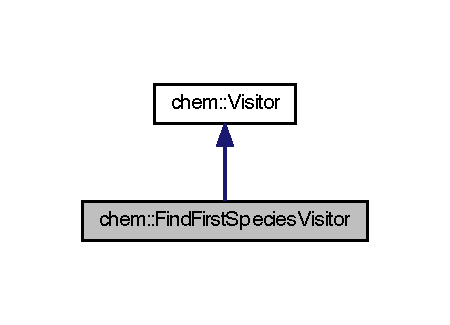
\includegraphics[width=216pt]{classchem_1_1FindFirstSpeciesVisitor__inherit__graph}
\end{center}
\end{figure}


Collaboration diagram for chem\-:\-:Find\-First\-Species\-Visitor\-:\nopagebreak
\begin{figure}[H]
\begin{center}
\leavevmode
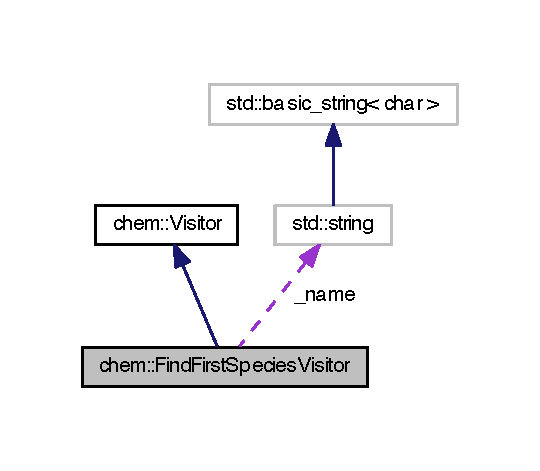
\includegraphics[width=259pt]{classchem_1_1FindFirstSpeciesVisitor__coll__graph}
\end{center}
\end{figure}
\subsection*{Public Member Functions}
\begin{DoxyCompactItemize}
\item 
\hyperlink{classchem_1_1FindFirstSpeciesVisitor_afaec67740a4522c9bd189b70c86f2852}{Find\-First\-Species\-Visitor} (const std\-::string \&name)
\item 
virtual bool \hyperlink{classchem_1_1FindFirstSpeciesVisitor_afe2b8f520e443307a6ba06a24c4b9991}{visit} (\hyperlink{classchem_1_1Component}{Component} $\ast$c)
\end{DoxyCompactItemize}
\subsection*{Private Attributes}
\begin{DoxyCompactItemize}
\item 
std\-::string \hyperlink{classchem_1_1FindFirstSpeciesVisitor_ae3fce85495fc42ef9a9bfea2117cdc12}{\-\_\-name}
\end{DoxyCompactItemize}


\subsection{Detailed Description}


Definition at line 29 of file Visitor\-Concrete.\-h.



\subsection{Constructor \& Destructor Documentation}
\hypertarget{classchem_1_1FindFirstSpeciesVisitor_afaec67740a4522c9bd189b70c86f2852}{\index{chem\-::\-Find\-First\-Species\-Visitor@{chem\-::\-Find\-First\-Species\-Visitor}!Find\-First\-Species\-Visitor@{Find\-First\-Species\-Visitor}}
\index{Find\-First\-Species\-Visitor@{Find\-First\-Species\-Visitor}!chem::FindFirstSpeciesVisitor@{chem\-::\-Find\-First\-Species\-Visitor}}
\subsubsection[{Find\-First\-Species\-Visitor}]{\setlength{\rightskip}{0pt plus 5cm}{\bf chem\-::\-Find\-First\-Species\-Visitor\-::\-Find\-First\-Species\-Visitor} (
\begin{DoxyParamCaption}
\item[{const std\-::string \&}]{name}
\end{DoxyParamCaption}
)\hspace{0.3cm}{\ttfamily  \mbox{[}inline\mbox{]}}}}\label{classchem_1_1FindFirstSpeciesVisitor_afaec67740a4522c9bd189b70c86f2852}


Definition at line 33 of file Visitor\-Concrete.\-h.



\subsection{Member Function Documentation}
\hypertarget{classchem_1_1FindFirstSpeciesVisitor_afe2b8f520e443307a6ba06a24c4b9991}{\index{chem\-::\-Find\-First\-Species\-Visitor@{chem\-::\-Find\-First\-Species\-Visitor}!visit@{visit}}
\index{visit@{visit}!chem::FindFirstSpeciesVisitor@{chem\-::\-Find\-First\-Species\-Visitor}}
\subsubsection[{visit}]{\setlength{\rightskip}{0pt plus 5cm}virtual bool {\bf chem\-::\-Find\-First\-Species\-Visitor\-::visit} (
\begin{DoxyParamCaption}
\item[{{\bf Component} $\ast$}]{c}
\end{DoxyParamCaption}
)\hspace{0.3cm}{\ttfamily  \mbox{[}inline, virtual\mbox{]}}}}\label{classchem_1_1FindFirstSpeciesVisitor_afe2b8f520e443307a6ba06a24c4b9991}


Implements \hyperlink{classchem_1_1Visitor_a3a148d3144ed2ef25972509a6a594d1a}{chem\-::\-Visitor}.



Definition at line 34 of file Visitor\-Concrete.\-h.



References \-\_\-name.



\subsection{Member Data Documentation}
\hypertarget{classchem_1_1FindFirstSpeciesVisitor_ae3fce85495fc42ef9a9bfea2117cdc12}{\index{chem\-::\-Find\-First\-Species\-Visitor@{chem\-::\-Find\-First\-Species\-Visitor}!\-\_\-name@{\-\_\-name}}
\index{\-\_\-name@{\-\_\-name}!chem::FindFirstSpeciesVisitor@{chem\-::\-Find\-First\-Species\-Visitor}}
\subsubsection[{\-\_\-name}]{\setlength{\rightskip}{0pt plus 5cm}std\-::string {\bf chem\-::\-Find\-First\-Species\-Visitor\-::\-\_\-name}\hspace{0.3cm}{\ttfamily  \mbox{[}private\mbox{]}}}}\label{classchem_1_1FindFirstSpeciesVisitor_ae3fce85495fc42ef9a9bfea2117cdc12}


Definition at line 31 of file Visitor\-Concrete.\-h.



Referenced by visit().



The documentation for this class was generated from the following file\-:\begin{DoxyCompactItemize}
\item 
Cyto\-Sim/\hyperlink{VisitorConcrete_8h}{Visitor\-Concrete.\-h}\end{DoxyCompactItemize}

\hypertarget{classchem_1_1PQNode}{\section{chem\-:\-:P\-Q\-Node Class Reference}
\label{classchem_1_1PQNode}\index{chem\-::\-P\-Q\-Node@{chem\-::\-P\-Q\-Node}}
}


\hyperlink{classchem_1_1PQNode}{P\-Q\-Node} stands for Priority Queue Node.  




{\ttfamily \#include $<$Chem\-N\-R\-M\-Impl.\-h$>$}



Collaboration diagram for chem\-:\-:P\-Q\-Node\-:
\nopagebreak
\begin{figure}[H]
\begin{center}
\leavevmode
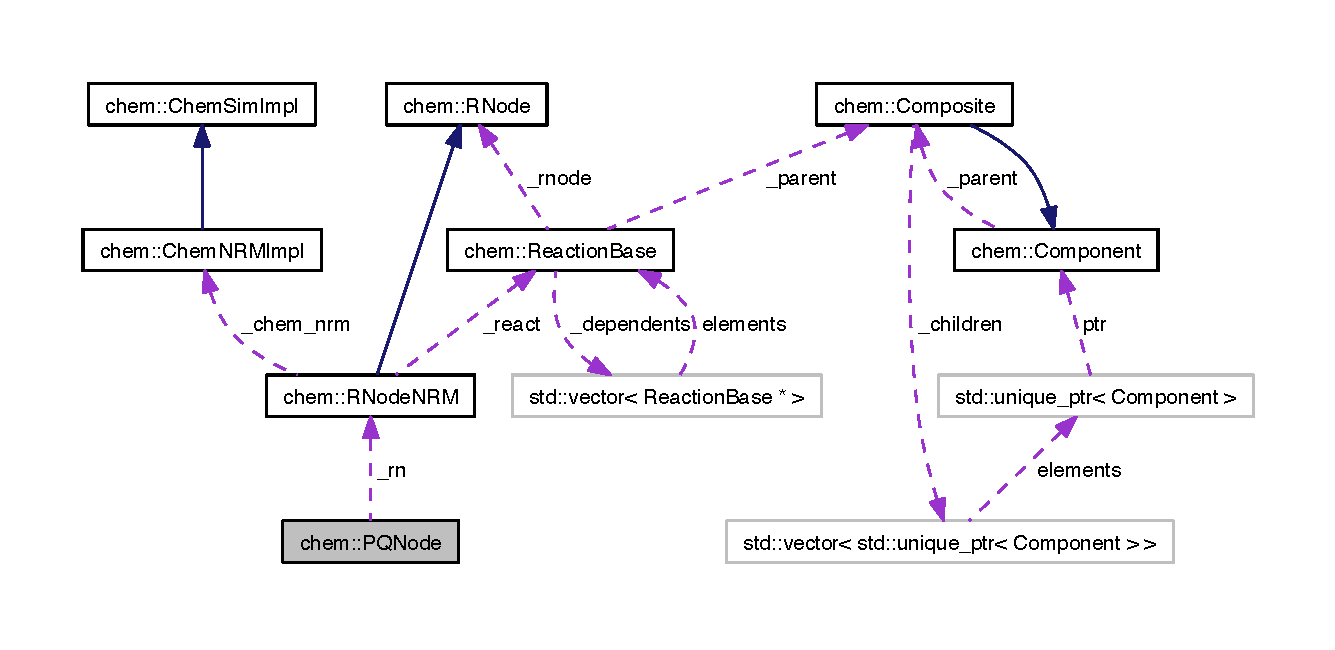
\includegraphics[width=350pt]{classchem_1_1PQNode__coll__graph}
\end{center}
\end{figure}
\subsection*{Public Member Functions}
\begin{DoxyCompactItemize}
\item 
\hyperlink{classchem_1_1PQNode_a216292a150c44b3f2bfeca4518663663}{P\-Q\-Node} (\hyperlink{classchem_1_1RNodeNRM}{R\-Node\-N\-R\-M} $\ast$rnode)
\begin{DoxyCompactList}\small\item\em Ctor. \end{DoxyCompactList}\item 
\hyperlink{classchem_1_1PQNode_a12604503b292d71658be54c9952afcbd}{$\sim$\-P\-Q\-Node} ()
\begin{DoxyCompactList}\small\item\em Dtor\-: we only reassign \-\_\-rn to null, the actual pointer needs to be deleted somewhere else to avoid memory leaks. \end{DoxyCompactList}\item 
bool \hyperlink{classchem_1_1PQNode_a0ba52697bcbc5b2c4accb7dece0aff24}{operator$<$} (\hyperlink{classchem_1_1PQNode}{P\-Q\-Node} const \&rhs) const 
\begin{DoxyCompactList}\small\item\em The P\-Q heap requires a comparision operator for ordering elements within the heap/. \end{DoxyCompactList}\item 
void $\ast$ \hyperlink{classchem_1_1PQNode_a1364ee21435946152266840256b8dd3f}{operator new} (std\-::size\-\_\-t size)
\begin{DoxyCompactList}\small\item\em Advanced memory management. \end{DoxyCompactList}\item 
void \hyperlink{classchem_1_1PQNode_af127d116cdefe86ba41005ef691affc1}{operator delete} (void $\ast$ptr) noexcept
\end{DoxyCompactItemize}
\subsection*{Private Attributes}
\begin{DoxyCompactItemize}
\item 
\hyperlink{classchem_1_1RNodeNRM}{R\-Node\-N\-R\-M} $\ast$ \hyperlink{classchem_1_1PQNode_ae0ddd94f908ec800ae02f592e83c630d}{\-\_\-rn}
\begin{DoxyCompactList}\small\item\em Pointer to the reaction node (\hyperlink{classchem_1_1RNodeNRM}{R\-Node\-N\-R\-M}) which this \hyperlink{classchem_1_1PQNode}{P\-Q\-Node} represents (or tracks) \end{DoxyCompactList}\item 
double \hyperlink{classchem_1_1PQNode_a77a83fe486c496c3e4bd4ffa72d8fb57}{\-\_\-tau}
\begin{DoxyCompactList}\small\item\em tau for this reaction for the Gibson-\/\-Bruck N\-R\-M algoritm \end{DoxyCompactList}\end{DoxyCompactItemize}
\subsection*{Friends}
\begin{DoxyCompactItemize}
\item 
class \hyperlink{classchem_1_1PQNode_a6dae39f8dddcdbda9b4f6a1c1bf1bda8}{Chem\-N\-R\-M\-Impl}
\item 
class \hyperlink{classchem_1_1PQNode_a9dfcd0d41325e8ca108cba1768ebab89}{R\-Node\-N\-R\-M}
\end{DoxyCompactItemize}


\subsection{Detailed Description}
\hyperlink{classchem_1_1PQNode}{P\-Q\-Node} stands for Priority Queue Node. 

It is stored as an element of a heap, such as boost\-::heap\-::pairing\-\_\-heap$<$\-P\-Q\-Node$>$. There will be an associated heap handle which can be used to dynamically access \hyperlink{classchem_1_1PQNode}{P\-Q\-Node}'s fields (e.\-g. boost\-::heap\-::pairing\-\_\-heap$<$\-P\-Q\-Node$>$\-::handle\-\_\-type)

This is a simple structure which holds a pointer to \hyperlink{classchem_1_1RNodeNRM}{R\-Node\-N\-R\-M} and stores the last computed tau assoicated with this reaction. On some occasions tau needs to be recomputed, for example when another reaction took place which affects this reaction. handle\-\_\-t of the corresponding heap element is used to get access to tau (and \hyperlink{classchem_1_1RNodeNRM}{R\-Node\-N\-R\-M}). 

Definition at line 59 of file Chem\-N\-R\-M\-Impl.\-h.



\subsection{Constructor \& Destructor Documentation}
\hypertarget{classchem_1_1PQNode_a216292a150c44b3f2bfeca4518663663}{\index{chem\-::\-P\-Q\-Node@{chem\-::\-P\-Q\-Node}!P\-Q\-Node@{P\-Q\-Node}}
\index{P\-Q\-Node@{P\-Q\-Node}!chem::PQNode@{chem\-::\-P\-Q\-Node}}
\subsubsection[{P\-Q\-Node}]{\setlength{\rightskip}{0pt plus 5cm}{\bf chem\-::\-P\-Q\-Node\-::\-P\-Q\-Node} (
\begin{DoxyParamCaption}
\item[{{\bf R\-Node\-N\-R\-M} $\ast$}]{rnode}
\end{DoxyParamCaption}
)\hspace{0.3cm}{\ttfamily  \mbox{[}inline\mbox{]}}}}\label{classchem_1_1PQNode_a216292a150c44b3f2bfeca4518663663}


Ctor. 


\begin{DoxyParams}{Parameters}
{\em $\ast$rnode} & is a pointer to the \hyperlink{classchem_1_1RNodeNRM}{R\-Node\-N\-R\-M} instance which this \hyperlink{classchem_1_1PQNode}{P\-Q\-Node} tracks (no ownership -\/ make sure it is not null) \\
\hline
\end{DoxyParams}
\begin{DoxyNote}{Note}
tau is set to infinity in the constructor 
\end{DoxyNote}


Definition at line 64 of file Chem\-N\-R\-M\-Impl.\-h.

\hypertarget{classchem_1_1PQNode_a12604503b292d71658be54c9952afcbd}{\index{chem\-::\-P\-Q\-Node@{chem\-::\-P\-Q\-Node}!$\sim$\-P\-Q\-Node@{$\sim$\-P\-Q\-Node}}
\index{$\sim$\-P\-Q\-Node@{$\sim$\-P\-Q\-Node}!chem::PQNode@{chem\-::\-P\-Q\-Node}}
\subsubsection[{$\sim$\-P\-Q\-Node}]{\setlength{\rightskip}{0pt plus 5cm}{\bf chem\-::\-P\-Q\-Node\-::$\sim$\-P\-Q\-Node} (
\begin{DoxyParamCaption}
{}
\end{DoxyParamCaption}
)\hspace{0.3cm}{\ttfamily  \mbox{[}inline\mbox{]}}}}\label{classchem_1_1PQNode_a12604503b292d71658be54c9952afcbd}


Dtor\-: we only reassign \-\_\-rn to null, the actual pointer needs to be deleted somewhere else to avoid memory leaks. 



Definition at line 67 of file Chem\-N\-R\-M\-Impl.\-h.



References \-\_\-rn.



\subsection{Member Function Documentation}
\hypertarget{classchem_1_1PQNode_af127d116cdefe86ba41005ef691affc1}{\index{chem\-::\-P\-Q\-Node@{chem\-::\-P\-Q\-Node}!operator delete@{operator delete}}
\index{operator delete@{operator delete}!chem::PQNode@{chem\-::\-P\-Q\-Node}}
\subsubsection[{operator delete}]{\setlength{\rightskip}{0pt plus 5cm}void chem\-::\-P\-Q\-Node\-::operator delete (
\begin{DoxyParamCaption}
\item[{void $\ast$}]{ptr}
\end{DoxyParamCaption}
)}}\label{classchem_1_1PQNode_af127d116cdefe86ba41005ef691affc1}


Definition at line 46 of file Chem\-N\-R\-M\-Impl.\-cpp.

\hypertarget{classchem_1_1PQNode_a1364ee21435946152266840256b8dd3f}{\index{chem\-::\-P\-Q\-Node@{chem\-::\-P\-Q\-Node}!operator new@{operator new}}
\index{operator new@{operator new}!chem::PQNode@{chem\-::\-P\-Q\-Node}}
\subsubsection[{operator new}]{\setlength{\rightskip}{0pt plus 5cm}void $\ast$ chem\-::\-P\-Q\-Node\-::operator new (
\begin{DoxyParamCaption}
\item[{std\-::size\-\_\-t}]{size}
\end{DoxyParamCaption}
)}}\label{classchem_1_1PQNode_a1364ee21435946152266840256b8dd3f}


Advanced memory management. 



Definition at line 38 of file Chem\-N\-R\-M\-Impl.\-cpp.

\hypertarget{classchem_1_1PQNode_a0ba52697bcbc5b2c4accb7dece0aff24}{\index{chem\-::\-P\-Q\-Node@{chem\-::\-P\-Q\-Node}!operator$<$@{operator$<$}}
\index{operator$<$@{operator$<$}!chem::PQNode@{chem\-::\-P\-Q\-Node}}
\subsubsection[{operator$<$}]{\setlength{\rightskip}{0pt plus 5cm}bool chem\-::\-P\-Q\-Node\-::operator$<$ (
\begin{DoxyParamCaption}
\item[{{\bf P\-Q\-Node} const \&}]{rhs}
\end{DoxyParamCaption}
) const\hspace{0.3cm}{\ttfamily  \mbox{[}inline\mbox{]}}}}\label{classchem_1_1PQNode_a0ba52697bcbc5b2c4accb7dece0aff24}


The P\-Q heap requires a comparision operator for ordering elements within the heap/. 

\begin{DoxyNote}{Note}
In a bit of hack, the less operator is actually defined via real greater comparison of tau's of two corresponding \hyperlink{classchem_1_1PQNode}{P\-Q\-Node} objects. We do this so the top P\-Q node has the smallest tau and not largest. 
\end{DoxyNote}


Definition at line 72 of file Chem\-N\-R\-M\-Impl.\-h.



References \-\_\-tau.



\subsection{Friends And Related Function Documentation}
\hypertarget{classchem_1_1PQNode_a6dae39f8dddcdbda9b4f6a1c1bf1bda8}{\index{chem\-::\-P\-Q\-Node@{chem\-::\-P\-Q\-Node}!Chem\-N\-R\-M\-Impl@{Chem\-N\-R\-M\-Impl}}
\index{Chem\-N\-R\-M\-Impl@{Chem\-N\-R\-M\-Impl}!chem::PQNode@{chem\-::\-P\-Q\-Node}}
\subsubsection[{Chem\-N\-R\-M\-Impl}]{\setlength{\rightskip}{0pt plus 5cm}friend class {\bf Chem\-N\-R\-M\-Impl}\hspace{0.3cm}{\ttfamily  \mbox{[}friend\mbox{]}}}}\label{classchem_1_1PQNode_a6dae39f8dddcdbda9b4f6a1c1bf1bda8}


Definition at line 89 of file Chem\-N\-R\-M\-Impl.\-h.

\hypertarget{classchem_1_1PQNode_a9dfcd0d41325e8ca108cba1768ebab89}{\index{chem\-::\-P\-Q\-Node@{chem\-::\-P\-Q\-Node}!R\-Node\-N\-R\-M@{R\-Node\-N\-R\-M}}
\index{R\-Node\-N\-R\-M@{R\-Node\-N\-R\-M}!chem::PQNode@{chem\-::\-P\-Q\-Node}}
\subsubsection[{R\-Node\-N\-R\-M}]{\setlength{\rightskip}{0pt plus 5cm}friend class {\bf R\-Node\-N\-R\-M}\hspace{0.3cm}{\ttfamily  \mbox{[}friend\mbox{]}}}}\label{classchem_1_1PQNode_a9dfcd0d41325e8ca108cba1768ebab89}


Definition at line 90 of file Chem\-N\-R\-M\-Impl.\-h.



\subsection{Member Data Documentation}
\hypertarget{classchem_1_1PQNode_ae0ddd94f908ec800ae02f592e83c630d}{\index{chem\-::\-P\-Q\-Node@{chem\-::\-P\-Q\-Node}!\-\_\-rn@{\-\_\-rn}}
\index{\-\_\-rn@{\-\_\-rn}!chem::PQNode@{chem\-::\-P\-Q\-Node}}
\subsubsection[{\-\_\-rn}]{\setlength{\rightskip}{0pt plus 5cm}{\bf R\-Node\-N\-R\-M}$\ast$ {\bf chem\-::\-P\-Q\-Node\-::\-\_\-rn}\hspace{0.3cm}{\ttfamily  \mbox{[}private\mbox{]}}}}\label{classchem_1_1PQNode_ae0ddd94f908ec800ae02f592e83c630d}


Pointer to the reaction node (\hyperlink{classchem_1_1RNodeNRM}{R\-Node\-N\-R\-M}) which this \hyperlink{classchem_1_1PQNode}{P\-Q\-Node} represents (or tracks) 



Definition at line 85 of file Chem\-N\-R\-M\-Impl.\-h.



Referenced by $\sim$\-P\-Q\-Node().

\hypertarget{classchem_1_1PQNode_a77a83fe486c496c3e4bd4ffa72d8fb57}{\index{chem\-::\-P\-Q\-Node@{chem\-::\-P\-Q\-Node}!\-\_\-tau@{\-\_\-tau}}
\index{\-\_\-tau@{\-\_\-tau}!chem::PQNode@{chem\-::\-P\-Q\-Node}}
\subsubsection[{\-\_\-tau}]{\setlength{\rightskip}{0pt plus 5cm}double {\bf chem\-::\-P\-Q\-Node\-::\-\_\-tau}\hspace{0.3cm}{\ttfamily  \mbox{[}private\mbox{]}}}}\label{classchem_1_1PQNode_a77a83fe486c496c3e4bd4ffa72d8fb57}


tau for this reaction for the Gibson-\/\-Bruck N\-R\-M algoritm 



Definition at line 86 of file Chem\-N\-R\-M\-Impl.\-h.



Referenced by operator$<$().



The documentation for this class was generated from the following files\-:\begin{DoxyCompactItemize}
\item 
Cyto\-Sim/\hyperlink{ChemNRMImpl_8h}{Chem\-N\-R\-M\-Impl.\-h}\item 
Cyto\-Sim/\hyperlink{ChemNRMImpl_8cpp}{Chem\-N\-R\-M\-Impl.\-cpp}\end{DoxyCompactItemize}

\hypertarget{classchem_1_1Reaction}{\section{chem\-:\-:Reaction Class Reference}
\label{classchem_1_1Reaction}\index{chem\-::\-Reaction@{chem\-::\-Reaction}}
}


\hyperlink{classchem_1_1Reaction}{Reaction} class represents simple chemical reactions of the form A + B -\/$>$ C.  




{\ttfamily \#include $<$Reaction.\-h$>$}



Collaboration diagram for chem\-:\-:Reaction\-:\nopagebreak
\begin{figure}[H]
\begin{center}
\leavevmode
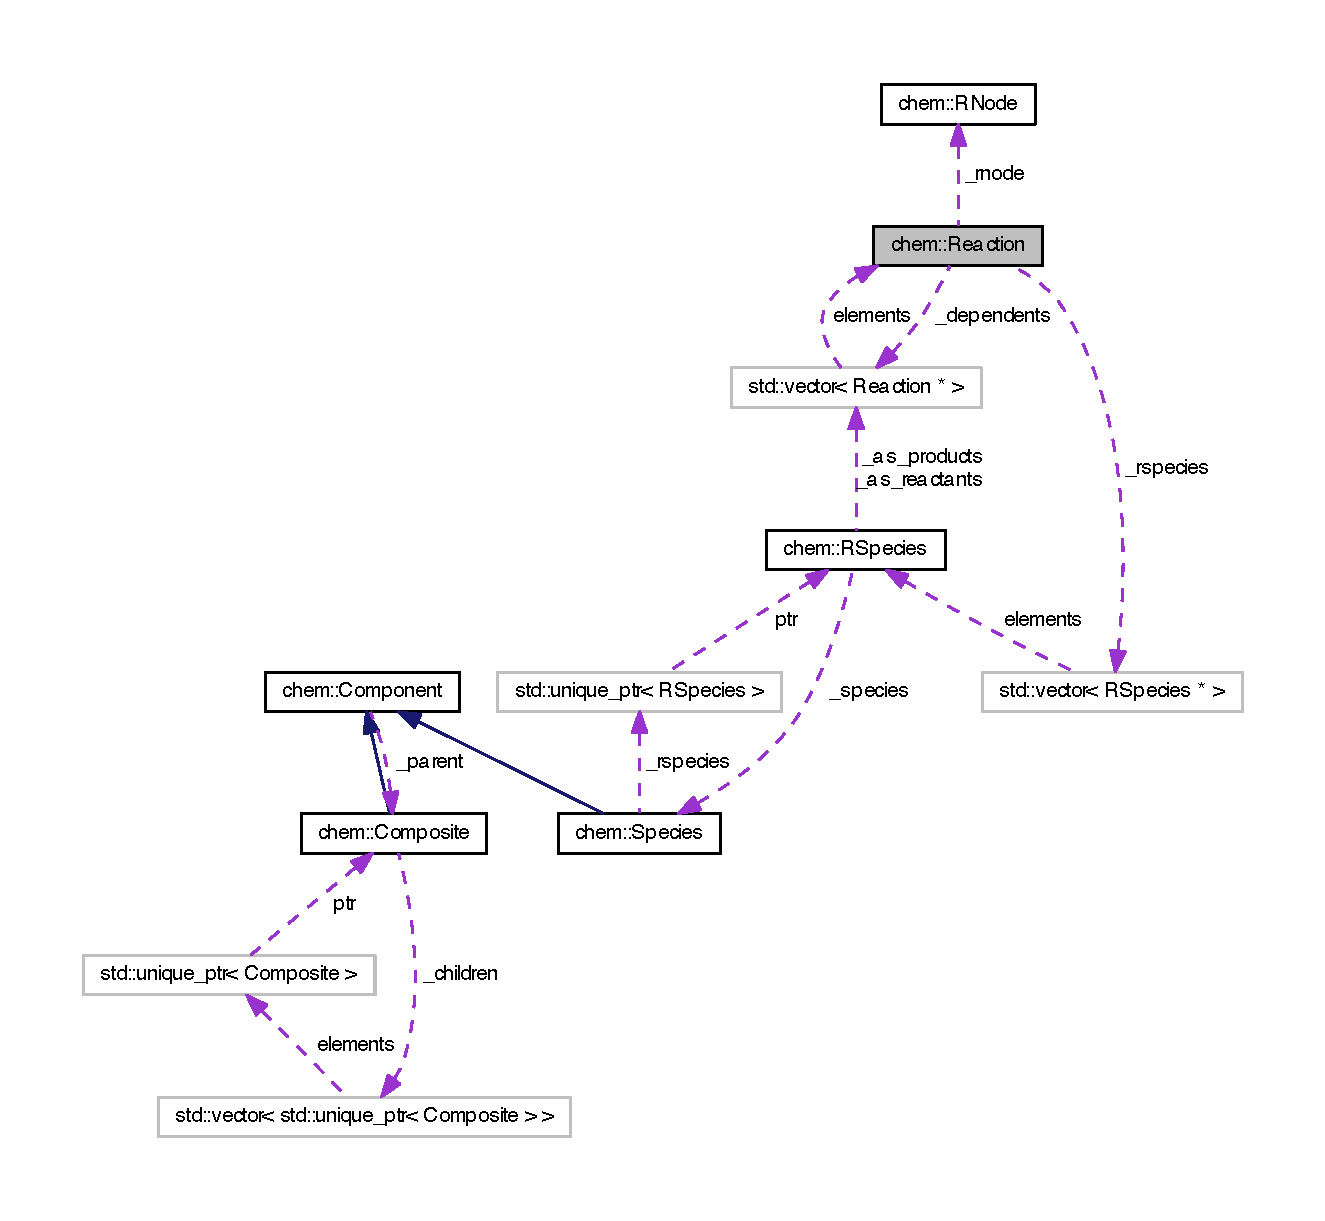
\includegraphics[width=350pt]{classchem_1_1Reaction__coll__graph}
\end{center}
\end{figure}
\subsection*{Public Member Functions}
\begin{DoxyCompactItemize}
\item 
\hyperlink{classchem_1_1Reaction_a357e31612d0c232d22bb3673fffb75c2}{Reaction} (std\-::initializer\-\_\-list$<$ \hyperlink{classchem_1_1Species}{Species} $\ast$ $>$ species, unsigned char M, unsigned char N, float rate)
\begin{DoxyCompactList}\small\item\em The main constructor\-: \end{DoxyCompactList}\item 
\hyperlink{classchem_1_1Reaction_a6557de5f31aa20434edc8ff2c780a71e}{Reaction} (const \hyperlink{classchem_1_1Reaction}{Reaction} \&r)
\item 
\hyperlink{classchem_1_1Reaction}{Reaction} \& \hyperlink{classchem_1_1Reaction_ae0c7b46c61af874a03ce6d826884711b}{operator=} (\hyperlink{classchem_1_1Reaction}{Reaction} \&r)
\item 
\hyperlink{classchem_1_1Reaction_a54eb494f216da7e4b462885d7715fc39}{$\sim$\-Reaction} ()
\begin{DoxyCompactList}\small\item\em Destructor. \end{DoxyCompactList}\item 
void \hyperlink{classchem_1_1Reaction_aad9d07693c386d626a9cd1eaf64ad507}{set\-Rate} (float rate)
\begin{DoxyCompactList}\small\item\em Sets the reaction rate to the parameter \char`\"{}rate\char`\"{}. \end{DoxyCompactList}\item 
void \hyperlink{classchem_1_1Reaction_a5a7d582d4c2f5a447da9844a0e4c5f97}{set\-Rnode} (\hyperlink{classchem_1_1RNode}{R\-Node} $\ast$rhs)
\begin{DoxyCompactList}\small\item\em Sets the \hyperlink{classchem_1_1RNode}{R\-Node} pointer associated with this \hyperlink{classchem_1_1Reaction}{Reaction} to rhs. \end{DoxyCompactList}\item 
float \hyperlink{classchem_1_1Reaction_a4661af0fbf33c822ba8ee530a8498ae7}{get\-Rate} () const 
\begin{DoxyCompactList}\small\item\em Returns the rate associated with this \hyperlink{classchem_1_1Reaction}{Reaction}. \end{DoxyCompactList}\item 
\hyperlink{classchem_1_1RNode}{R\-Node} $\ast$ \hyperlink{classchem_1_1Reaction_af12e3997f13ccb476f7bac45297f4ff9}{get\-Rnode} () const 
\begin{DoxyCompactList}\small\item\em Returns a pointer to the \hyperlink{classchem_1_1RNode}{R\-Node} associated with this \hyperlink{classchem_1_1Reaction}{Reaction}. \end{DoxyCompactList}\item 
unsigned char \hyperlink{classchem_1_1Reaction_a5f420aec9fb36444175089ab16ddb141}{get\-M} () const 
\begin{DoxyCompactList}\small\item\em Returns the number of reactant \hyperlink{classchem_1_1RSpecies}{R\-Species}. \end{DoxyCompactList}\item 
unsigned char \hyperlink{classchem_1_1Reaction_a35c63f46973b5cda157661ab9bffb682}{get\-N} () const 
\begin{DoxyCompactList}\small\item\em Returns the number of product \hyperlink{classchem_1_1RSpecies}{R\-Species}. \end{DoxyCompactList}\item 
int \hyperlink{classchem_1_1Reaction_adffedea2cba0124feda82ef9e3cee5e7}{get\-Product\-Of\-Reactants} () const 
\begin{DoxyCompactList}\small\item\em Computes the product of the copy number of all reactant \hyperlink{classchem_1_1RSpecies}{R\-Species}. \end{DoxyCompactList}\item 
int \hyperlink{classchem_1_1Reaction_aa2dcaea0bc0893a3c00cb3cbcd0a2d6c}{get\-Product\-Of\-Products} () const 
\begin{DoxyCompactList}\small\item\em Computes the product of the copy number of all product \hyperlink{classchem_1_1RSpecies}{R\-Species} minus maxium allowed copy number. \end{DoxyCompactList}\item 
bool \hyperlink{classchem_1_1Reaction_a6c03b9b74a8da07b51a6924bfe2f9571}{is\-Passivated} () const 
\begin{DoxyCompactList}\small\item\em Return true if the \hyperlink{classchem_1_1Reaction}{Reaction} is currently passivated. \end{DoxyCompactList}\item 
bool \hyperlink{classchem_1_1Reaction_a316db368606eb9aaf47dfbde6d48f606}{is\-Signaling} () const 
\begin{DoxyCompactList}\small\item\em Return true if this \hyperlink{classchem_1_1RSpecies}{R\-Species} emits signals on copy number change. \end{DoxyCompactList}\item 
void \hyperlink{classchem_1_1Reaction_a584613fe0d634660a1814744c76a4208}{start\-Signaling} ()
\begin{DoxyCompactList}\small\item\em Set the signaling behavior of this \hyperlink{classchem_1_1Reaction}{Reaction}. \end{DoxyCompactList}\item 
void \hyperlink{classchem_1_1Reaction_ace48838b7b1bac957e840ad7b2f4a4e1}{stop\-Signaling} ()
\begin{DoxyCompactList}\small\item\em Destroy the signal associated with this \hyperlink{classchem_1_1Reaction}{Reaction}; all associated slots will be destroyed. \end{DoxyCompactList}\item 
boost\-::signals2\-::connection \hyperlink{classchem_1_1Reaction_af427c88bd882105d317f99d5a9f4a34d}{connect} (std\-::function$<$ void(\hyperlink{classchem_1_1Reaction}{Reaction} $\ast$)$>$ const \&react\-\_\-callback, int priority=5)
\begin{DoxyCompactList}\small\item\em Connect the callback, react\-\_\-callback to a signal corresponding to \hyperlink{classchem_1_1Reaction}{Reaction} $\ast$r. \end{DoxyCompactList}\item 
void \hyperlink{classchem_1_1Reaction_ab76db5606306efa0772f7833a5f2ce68}{emit\-Signal} ()
\begin{DoxyCompactList}\small\item\em Broadcasts signal indicating that the \hyperlink{classchem_1_1Reaction}{Reaction} event has taken place This method is only called by the code which runs the chemical dynamics (i.\-e. \end{DoxyCompactList}\item 
const std\-::vector$<$ \hyperlink{classchem_1_1Reaction}{Reaction} $\ast$ $>$ \& \hyperlink{classchem_1_1Reaction_af001778d48ac0800beba1b7031aeab33}{dependents} ()
\begin{DoxyCompactList}\small\item\em Return a const reference to the vector of dependent reactions. \end{DoxyCompactList}\item 
\hyperlink{namespacechem_a9b02b32d43473a3cd87fd30f910cc121}{vrsp\-\_\-iterator} \hyperlink{classchem_1_1Reaction_a7637b6f060d8d1ca859d89966ccfd39e}{begin\-Reactants} ()
\item 
\hyperlink{namespacechem_ab6ba36c9953625b15ff4105e1cdfdb86}{vrsp\-\_\-const\-\_\-iterator} \hyperlink{classchem_1_1Reaction_a84a70eef65b79375f92a0b702883da54}{cbegin\-Reactants} () const 
\item 
\hyperlink{namespacechem_a9b02b32d43473a3cd87fd30f910cc121}{vrsp\-\_\-iterator} \hyperlink{classchem_1_1Reaction_a14336488f8477a51295ae8a6e68aacda}{end\-Reactants} ()
\item 
\hyperlink{namespacechem_ab6ba36c9953625b15ff4105e1cdfdb86}{vrsp\-\_\-const\-\_\-iterator} \hyperlink{classchem_1_1Reaction_a0df8820ef13d8ba3014b610b1aeeed9e}{cend\-Reactants} () const 
\item 
\hyperlink{namespacechem_a9b02b32d43473a3cd87fd30f910cc121}{vrsp\-\_\-iterator} \hyperlink{classchem_1_1Reaction_abd8e1fd6c8f8d247896fc15ebdd02dbc}{begin\-Products} ()
\item 
\hyperlink{namespacechem_ab6ba36c9953625b15ff4105e1cdfdb86}{vrsp\-\_\-const\-\_\-iterator} \hyperlink{classchem_1_1Reaction_a369a58328dc07d471ab884924872ba4d}{cbegin\-Products} () const 
\item 
\hyperlink{namespacechem_a9b02b32d43473a3cd87fd30f910cc121}{vrsp\-\_\-iterator} \hyperlink{classchem_1_1Reaction_a3d432b1719243cf0bb3259071c488afd}{end\-Products} ()
\item 
\hyperlink{namespacechem_ab6ba36c9953625b15ff4105e1cdfdb86}{vrsp\-\_\-const\-\_\-iterator} \hyperlink{classchem_1_1Reaction_a666cd5d81c28e29af77cabcbd3846540}{cend\-Products} () const 
\item 
void \hyperlink{classchem_1_1Reaction_a1341d466157788c3d547da52c6c59502}{make\-Step} ()
\begin{DoxyCompactList}\small\item\em Fire the \hyperlink{classchem_1_1Reaction}{Reaction} -\/ make a single step, where reactant \hyperlink{classchem_1_1RSpecies}{R\-Species} copy numbers are decreased by one, and the product \hyperlink{classchem_1_1RSpecies}{R\-Species} copy numbers are increased by one. \end{DoxyCompactList}\item 
float \hyperlink{classchem_1_1Reaction_a676eec8b5b28c191c555a944a2c03857}{compute\-Propensity} () const 
\begin{DoxyCompactList}\small\item\em Compute the \hyperlink{classchem_1_1Reaction}{Reaction} propensity that is needed by a Gillespie like algorithm\-: rate$\ast$reactant\-\_\-1.\hyperlink{classchem_1_1Reaction_a35c63f46973b5cda157661ab9bffb682}{get\-N()}$\ast$reactant\-\_\-2.\hyperlink{classchem_1_1Reaction_a35c63f46973b5cda157661ab9bffb682}{get\-N()}... \end{DoxyCompactList}\item 
void \hyperlink{classchem_1_1Reaction_a6990bf5dfc31f04bcab6bda8392174aa}{passivate\-Reaction} ()
\begin{DoxyCompactList}\small\item\em Usually is applied to \hyperlink{classchem_1_1Reaction}{Reaction} objects with propensity of 0 (e.\-g. \end{DoxyCompactList}\item 
void \hyperlink{classchem_1_1Reaction_afae5d992f176c16a21ec38fcf3d83649}{activate\-Reaction} ()
\begin{DoxyCompactList}\small\item\em Requests that \hyperlink{classchem_1_1Reaction}{Reaction} objects that may affect this \hyperlink{classchem_1_1Reaction}{Reaction} to start tracking it, which can be used to follow \hyperlink{classchem_1_1Reaction}{Reaction} objects whose propensities change upong firing of some \hyperlink{classchem_1_1Reaction}{Reaction}. \end{DoxyCompactList}\item 
void \hyperlink{classchem_1_1Reaction_af46fe664df202767dfac016253942799}{print\-Dependents} ()
\begin{DoxyCompactList}\small\item\em Print the Reactions that are affacted by this \hyperlink{classchem_1_1Reaction}{Reaction} being fired. \end{DoxyCompactList}\item 
std\-::vector$<$ \hyperlink{classchem_1_1Reaction}{Reaction} $\ast$ $>$ \hyperlink{classchem_1_1Reaction_aff0f07aebff09a5f15f2bd6d17686016}{get\-Affected\-Reactions} ()
\begin{DoxyCompactList}\small\item\em Return the list of \hyperlink{classchem_1_1Reaction}{Reaction} objects that are affected when this \hyperlink{classchem_1_1Reaction}{Reaction} is fired. \end{DoxyCompactList}\item 
void \hyperlink{classchem_1_1Reaction_a9971edbe11bb8c6b3148cbee3a449872}{register\-New\-Dependent} (\hyperlink{classchem_1_1Reaction}{Reaction} $\ast$r)
\begin{DoxyCompactList}\small\item\em Request that the \hyperlink{classchem_1_1Reaction}{Reaction} $\ast$r adds this \hyperlink{classchem_1_1Reaction}{Reaction} to its list of dependents which it affects. \end{DoxyCompactList}\item 
void \hyperlink{classchem_1_1Reaction_ab31fe2ac310f8d17b1af649bcb70e050}{unregister\-Dependent} (\hyperlink{classchem_1_1Reaction}{Reaction} $\ast$r)
\begin{DoxyCompactList}\small\item\em Request that the \hyperlink{classchem_1_1Reaction}{Reaction} $\ast$r removes this \hyperlink{classchem_1_1Reaction}{Reaction} from its list of dependents which it affects. \end{DoxyCompactList}\end{DoxyCompactItemize}
\subsection*{Private Attributes}
\begin{DoxyCompactItemize}
\item 
std\-::vector$<$ \hyperlink{classchem_1_1RSpecies}{R\-Species} $\ast$ $>$ \hyperlink{classchem_1_1Reaction_a5a8f536126edeb82526f9ac31c3e3c6c}{\-\_\-rspecies}
\begin{DoxyCompactList}\small\item\em Reactants and products constituting this \hyperlink{classchem_1_1Reaction}{Reaction}. \end{DoxyCompactList}\item 
std\-::vector$<$ \hyperlink{classchem_1_1Reaction}{Reaction} $\ast$ $>$ \hyperlink{classchem_1_1Reaction_a10b1e663b3c3677064d2b466e3dca437}{\-\_\-dependents}
\begin{DoxyCompactList}\small\item\em Pointers to \hyperlink{classchem_1_1Reaction}{Reaction} objects that depend on this \hyperlink{classchem_1_1Reaction}{Reaction} being executed. \end{DoxyCompactList}\item 
\hyperlink{classchem_1_1RNode}{R\-Node} $\ast$ \hyperlink{classchem_1_1Reaction_ae10d6d1a25e37bc4b3b5df478094e745}{\-\_\-rnode}
\begin{DoxyCompactList}\small\item\em A pointer to an \hyperlink{classchem_1_1RNode}{R\-Node} object which is used to implement a Gillespie-\/like algorithm (e.\-g. N\-R\-M) \end{DoxyCompactList}\item 
float \hyperlink{classchem_1_1Reaction_a6c5cd99c16816bfcbee48b8c78a0efe5}{\-\_\-rate}
\begin{DoxyCompactList}\small\item\em the rate for this \hyperlink{classchem_1_1Reaction}{Reaction} \end{DoxyCompactList}\item 
const unsigned char \hyperlink{classchem_1_1Reaction_a07b3c7e8a82111c786144158bc3cb4e5}{\-\_\-m}
\begin{DoxyCompactList}\small\item\em indicates the number of reactants \end{DoxyCompactList}\item 
\hyperlink{namespacechem_a85c409cf931d658d253b62ab5ad35781}{Reaction\-Event\-Signal} $\ast$ \hyperlink{classchem_1_1Reaction_a55ca3408f31e6074775d6a8cb2a6b95b}{\-\_\-signal}
\begin{DoxyCompactList}\small\item\em Can be used to broadcast a signal associated with this \hyperlink{classchem_1_1Reaction}{Reaction} (usuall when a single step of this \hyperlink{classchem_1_1Reaction}{Reaction} occurs) \end{DoxyCompactList}\item 
bool \hyperlink{classchem_1_1Reaction_aa0151836a315ac001ef94277b126c329}{\-\_\-passivated}
\begin{DoxyCompactList}\small\item\em Indicates whether the \hyperlink{classchem_1_1Reaction}{Reaction} is currently passivated. \end{DoxyCompactList}\end{DoxyCompactItemize}
\subsection*{Friends}
\begin{DoxyCompactItemize}
\item 
std\-::ostream \& \hyperlink{classchem_1_1Reaction_adae3b3c285aa2beddbb06bab27f9398f}{operator$<$$<$} (std\-::ostream \&os, const \hyperlink{classchem_1_1Reaction}{Reaction} \&rr)
\begin{DoxyCompactList}\small\item\em Print self into an iostream. \end{DoxyCompactList}\end{DoxyCompactItemize}


\subsection{Detailed Description}
\hyperlink{classchem_1_1Reaction}{Reaction} class represents simple chemical reactions of the form A + B -\/$>$ C. 

\hyperlink{classchem_1_1Reaction}{Reaction} is defined in terms of reactant and product \hyperlink{classchem_1_1RSpecies}{R\-Species}. In the current implementation, the stoichiometric coefficents can only be one\-: i.\-e. A + B -\/$>$ C + D is allowed, but A + 2\-B -\/$>$ C + D is not allowed. Almost all chemical reactions are either unimolecular or bimolecular, so this restriction should not be too burdensom. Also, the \hyperlink{classchem_1_1Reaction}{Reaction} indicates a forward process only. For processes in both directions, e.\-g. A $<$-\/$>$ B, two Reactions objects need to be defined, corresponding to A-\/$>$B and B-\/$>$A.

A \hyperlink{classchem_1_1Reaction}{Reaction} tracks other \hyperlink{classchem_1_1Reaction}{Reaction} objects that are affected if this \hyperlink{classchem_1_1Reaction}{Reaction} is executed. A \hyperlink{classchem_1_1Reaction}{Reaction} may be set up such that it \char`\"{}signals\char`\"{} when a reaction event happens, in which case the corresponding callbacks are called. 

Definition at line 49 of file Reaction.\-h.



\subsection{Constructor \& Destructor Documentation}
\hypertarget{classchem_1_1Reaction_a357e31612d0c232d22bb3673fffb75c2}{\index{chem\-::\-Reaction@{chem\-::\-Reaction}!Reaction@{Reaction}}
\index{Reaction@{Reaction}!chem::Reaction@{chem\-::\-Reaction}}
\subsubsection[{Reaction}]{\setlength{\rightskip}{0pt plus 5cm}{\bf chem\-::\-Reaction\-::\-Reaction} (
\begin{DoxyParamCaption}
\item[{std\-::initializer\-\_\-list$<$ {\bf Species} $\ast$ $>$}]{species, }
\item[{unsigned char}]{M, }
\item[{unsigned char}]{N, }
\item[{float}]{rate}
\end{DoxyParamCaption}
)}}\label{classchem_1_1Reaction_a357e31612d0c232d22bb3673fffb75c2}


The main constructor\-: 


\begin{DoxyParams}{Parameters}
{\em \hyperlink{classchem_1_1Species}{Species}} & that are reactants and products are put together into a single list (starting from reactants) \\
\hline
{\em M} & -\/ number of reactants \\
\hline
{\em N} & -\/ number of products \\
\hline
{\em rate} & -\/ the rate constant for this reaction \\
\hline
\end{DoxyParams}


Definition at line 17 of file Reaction.\-cpp.



References \-\_\-dependents, \-\_\-rspecies, chem\-::\-R\-Species\-::add\-As\-Product(), chem\-::\-R\-Species\-::add\-As\-Reactant(), begin\-Products(), begin\-Reactants(), end\-Products(), end\-Reactants(), and get\-Affected\-Reactions().

\hypertarget{classchem_1_1Reaction_a6557de5f31aa20434edc8ff2c780a71e}{\index{chem\-::\-Reaction@{chem\-::\-Reaction}!Reaction@{Reaction}}
\index{Reaction@{Reaction}!chem::Reaction@{chem\-::\-Reaction}}
\subsubsection[{Reaction}]{\setlength{\rightskip}{0pt plus 5cm}{\bf chem\-::\-Reaction\-::\-Reaction} (
\begin{DoxyParamCaption}
\item[{const {\bf Reaction} \&}]{r}
\end{DoxyParamCaption}
)}}\label{classchem_1_1Reaction_a6557de5f31aa20434edc8ff2c780a71e}
\hypertarget{classchem_1_1Reaction_a54eb494f216da7e4b462885d7715fc39}{\index{chem\-::\-Reaction@{chem\-::\-Reaction}!$\sim$\-Reaction@{$\sim$\-Reaction}}
\index{$\sim$\-Reaction@{$\sim$\-Reaction}!chem::Reaction@{chem\-::\-Reaction}}
\subsubsection[{$\sim$\-Reaction}]{\setlength{\rightskip}{0pt plus 5cm}{\bf chem\-::\-Reaction\-::$\sim$\-Reaction} (
\begin{DoxyParamCaption}
{}
\end{DoxyParamCaption}
)}}\label{classchem_1_1Reaction_a54eb494f216da7e4b462885d7715fc39}


Destructor. 



Definition at line 32 of file Reaction.\-cpp.



References \-\_\-signal, begin\-Products(), begin\-Reactants(), end\-Products(), end\-Reactants(), chem\-::\-R\-Species\-::remove\-As\-Product(), and chem\-::\-R\-Species\-::remove\-As\-Reactant().



\subsection{Member Function Documentation}
\hypertarget{classchem_1_1Reaction_afae5d992f176c16a21ec38fcf3d83649}{\index{chem\-::\-Reaction@{chem\-::\-Reaction}!activate\-Reaction@{activate\-Reaction}}
\index{activate\-Reaction@{activate\-Reaction}!chem::Reaction@{chem\-::\-Reaction}}
\subsubsection[{activate\-Reaction}]{\setlength{\rightskip}{0pt plus 5cm}void {\bf chem\-::\-Reaction\-::activate\-Reaction} (
\begin{DoxyParamCaption}
{}
\end{DoxyParamCaption}
)}}\label{classchem_1_1Reaction_afae5d992f176c16a21ec38fcf3d83649}


Requests that \hyperlink{classchem_1_1Reaction}{Reaction} objects that may affect this \hyperlink{classchem_1_1Reaction}{Reaction} to start tracking it, which can be used to follow \hyperlink{classchem_1_1Reaction}{Reaction} objects whose propensities change upong firing of some \hyperlink{classchem_1_1Reaction}{Reaction}. 



Definition at line 63 of file Reaction.\-cpp.



References \-\_\-passivated, \-\_\-rnode, chem\-::\-R\-Node\-::activate\-Reaction(), begin\-Reactants(), end\-Reactants(), get\-Product\-Of\-Products(), and get\-Product\-Of\-Reactants().

\hypertarget{classchem_1_1Reaction_abd8e1fd6c8f8d247896fc15ebdd02dbc}{\index{chem\-::\-Reaction@{chem\-::\-Reaction}!begin\-Products@{begin\-Products}}
\index{begin\-Products@{begin\-Products}!chem::Reaction@{chem\-::\-Reaction}}
\subsubsection[{begin\-Products}]{\setlength{\rightskip}{0pt plus 5cm}{\bf vrsp\-\_\-iterator} {\bf chem\-::\-Reaction\-::begin\-Products} (
\begin{DoxyParamCaption}
{}
\end{DoxyParamCaption}
)\hspace{0.3cm}{\ttfamily  \mbox{[}inline\mbox{]}}}}\label{classchem_1_1Reaction_abd8e1fd6c8f8d247896fc15ebdd02dbc}


Definition at line 168 of file Reaction.\-h.



References \-\_\-m, and \-\_\-rspecies.



Referenced by make\-Step(), chem\-::\-Chem\-N\-R\-M\-Impl\-::make\-Step(), Reaction(), and $\sim$\-Reaction().

\hypertarget{classchem_1_1Reaction_a7637b6f060d8d1ca859d89966ccfd39e}{\index{chem\-::\-Reaction@{chem\-::\-Reaction}!begin\-Reactants@{begin\-Reactants}}
\index{begin\-Reactants@{begin\-Reactants}!chem::Reaction@{chem\-::\-Reaction}}
\subsubsection[{begin\-Reactants}]{\setlength{\rightskip}{0pt plus 5cm}{\bf vrsp\-\_\-iterator} {\bf chem\-::\-Reaction\-::begin\-Reactants} (
\begin{DoxyParamCaption}
{}
\end{DoxyParamCaption}
)\hspace{0.3cm}{\ttfamily  \mbox{[}inline\mbox{]}}}}\label{classchem_1_1Reaction_a7637b6f060d8d1ca859d89966ccfd39e}


Definition at line 156 of file Reaction.\-h.



References \-\_\-rspecies.



Referenced by activate\-Reaction(), make\-Step(), chem\-::\-Chem\-N\-R\-M\-Impl\-::make\-Step(), passivate\-Reaction(), Reaction(), and $\sim$\-Reaction().

\hypertarget{classchem_1_1Reaction_a369a58328dc07d471ab884924872ba4d}{\index{chem\-::\-Reaction@{chem\-::\-Reaction}!cbegin\-Products@{cbegin\-Products}}
\index{cbegin\-Products@{cbegin\-Products}!chem::Reaction@{chem\-::\-Reaction}}
\subsubsection[{cbegin\-Products}]{\setlength{\rightskip}{0pt plus 5cm}{\bf vrsp\-\_\-const\-\_\-iterator} {\bf chem\-::\-Reaction\-::cbegin\-Products} (
\begin{DoxyParamCaption}
{}
\end{DoxyParamCaption}
) const\hspace{0.3cm}{\ttfamily  \mbox{[}inline\mbox{]}}}}\label{classchem_1_1Reaction_a369a58328dc07d471ab884924872ba4d}


Definition at line 172 of file Reaction.\-h.



References \-\_\-m, and \-\_\-rspecies.



Referenced by get\-Product\-Of\-Products(), and chem\-::operator$<$$<$().

\hypertarget{classchem_1_1Reaction_a84a70eef65b79375f92a0b702883da54}{\index{chem\-::\-Reaction@{chem\-::\-Reaction}!cbegin\-Reactants@{cbegin\-Reactants}}
\index{cbegin\-Reactants@{cbegin\-Reactants}!chem::Reaction@{chem\-::\-Reaction}}
\subsubsection[{cbegin\-Reactants}]{\setlength{\rightskip}{0pt plus 5cm}{\bf vrsp\-\_\-const\-\_\-iterator} {\bf chem\-::\-Reaction\-::cbegin\-Reactants} (
\begin{DoxyParamCaption}
{}
\end{DoxyParamCaption}
) const\hspace{0.3cm}{\ttfamily  \mbox{[}inline\mbox{]}}}}\label{classchem_1_1Reaction_a84a70eef65b79375f92a0b702883da54}


Definition at line 159 of file Reaction.\-h.



References \-\_\-rspecies.



Referenced by compute\-Propensity(), get\-Product\-Of\-Reactants(), and chem\-::operator$<$$<$().

\hypertarget{classchem_1_1Reaction_a666cd5d81c28e29af77cabcbd3846540}{\index{chem\-::\-Reaction@{chem\-::\-Reaction}!cend\-Products@{cend\-Products}}
\index{cend\-Products@{cend\-Products}!chem::Reaction@{chem\-::\-Reaction}}
\subsubsection[{cend\-Products}]{\setlength{\rightskip}{0pt plus 5cm}{\bf vrsp\-\_\-const\-\_\-iterator} {\bf chem\-::\-Reaction\-::cend\-Products} (
\begin{DoxyParamCaption}
{}
\end{DoxyParamCaption}
) const\hspace{0.3cm}{\ttfamily  \mbox{[}inline\mbox{]}}}}\label{classchem_1_1Reaction_a666cd5d81c28e29af77cabcbd3846540}


Definition at line 178 of file Reaction.\-h.



References \-\_\-rspecies.



Referenced by get\-Product\-Of\-Products(), and chem\-::operator$<$$<$().

\hypertarget{classchem_1_1Reaction_a0df8820ef13d8ba3014b610b1aeeed9e}{\index{chem\-::\-Reaction@{chem\-::\-Reaction}!cend\-Reactants@{cend\-Reactants}}
\index{cend\-Reactants@{cend\-Reactants}!chem::Reaction@{chem\-::\-Reaction}}
\subsubsection[{cend\-Reactants}]{\setlength{\rightskip}{0pt plus 5cm}{\bf vrsp\-\_\-const\-\_\-iterator} {\bf chem\-::\-Reaction\-::cend\-Reactants} (
\begin{DoxyParamCaption}
{}
\end{DoxyParamCaption}
) const\hspace{0.3cm}{\ttfamily  \mbox{[}inline\mbox{]}}}}\label{classchem_1_1Reaction_a0df8820ef13d8ba3014b610b1aeeed9e}


Definition at line 165 of file Reaction.\-h.



References \-\_\-m, and \-\_\-rspecies.



Referenced by compute\-Propensity(), get\-Product\-Of\-Reactants(), and chem\-::operator$<$$<$().

\hypertarget{classchem_1_1Reaction_a676eec8b5b28c191c555a944a2c03857}{\index{chem\-::\-Reaction@{chem\-::\-Reaction}!compute\-Propensity@{compute\-Propensity}}
\index{compute\-Propensity@{compute\-Propensity}!chem::Reaction@{chem\-::\-Reaction}}
\subsubsection[{compute\-Propensity}]{\setlength{\rightskip}{0pt plus 5cm}float {\bf chem\-::\-Reaction\-::compute\-Propensity} (
\begin{DoxyParamCaption}
{}
\end{DoxyParamCaption}
) const\hspace{0.3cm}{\ttfamily  \mbox{[}inline\mbox{]}}}}\label{classchem_1_1Reaction_a676eec8b5b28c191c555a944a2c03857}


Compute the \hyperlink{classchem_1_1Reaction}{Reaction} propensity that is needed by a Gillespie like algorithm\-: rate$\ast$reactant\-\_\-1.\hyperlink{classchem_1_1Reaction_a35c63f46973b5cda157661ab9bffb682}{get\-N()}$\ast$reactant\-\_\-2.\hyperlink{classchem_1_1Reaction_a35c63f46973b5cda157661ab9bffb682}{get\-N()}... 



Definition at line 193 of file Reaction.\-h.



References \-\_\-rate, cbegin\-Reactants(), cend\-Reactants(), and chem\-::\-R\-Species\-::get\-N().



Referenced by chem\-::operator$<$$<$(), chem\-::\-R\-Node\-N\-R\-M\-::re\-Compute\-Propensity(), and chem\-::\-R\-Node\-N\-R\-M\-::\-R\-Node\-N\-R\-M().

\hypertarget{classchem_1_1Reaction_af427c88bd882105d317f99d5a9f4a34d}{\index{chem\-::\-Reaction@{chem\-::\-Reaction}!connect@{connect}}
\index{connect@{connect}!chem::Reaction@{chem\-::\-Reaction}}
\subsubsection[{connect}]{\setlength{\rightskip}{0pt plus 5cm}boost\-::signals2\-::connection {\bf chem\-::\-Reaction\-::connect} (
\begin{DoxyParamCaption}
\item[{std\-::function$<$ void({\bf Reaction} $\ast$)$>$ const \&}]{react\-\_\-callback, }
\item[{int}]{priority = {\ttfamily 5}}
\end{DoxyParamCaption}
)}}\label{classchem_1_1Reaction_af427c88bd882105d317f99d5a9f4a34d}


Connect the callback, react\-\_\-callback to a signal corresponding to \hyperlink{classchem_1_1Reaction}{Reaction} $\ast$r. 


\begin{DoxyParams}{Parameters}
{\em std\-::function$<$void} & (\hyperlink{classchem_1_1Reaction}{Reaction} $\ast$)$>$ const \&react\-\_\-callback -\/ a function object to be called (a slot) \\
\hline
{\em int} & priority -\/ lower priority slots will be called first. Default is 5 Do not use priorities 1 and 2 unless absolutely essential. \\
\hline
\end{DoxyParams}
\begin{DoxyReturn}{Returns}
a connection object which can be used to later disconnect this particular slot or temporarily block it 
\end{DoxyReturn}


Definition at line 114 of file Reaction.\-cpp.



References \-\_\-signal, is\-Signaling(), and start\-Signaling().

\hypertarget{classchem_1_1Reaction_af001778d48ac0800beba1b7031aeab33}{\index{chem\-::\-Reaction@{chem\-::\-Reaction}!dependents@{dependents}}
\index{dependents@{dependents}!chem::Reaction@{chem\-::\-Reaction}}
\subsubsection[{dependents}]{\setlength{\rightskip}{0pt plus 5cm}const std\-::vector$<${\bf Reaction}$\ast$$>$\& {\bf chem\-::\-Reaction\-::dependents} (
\begin{DoxyParamCaption}
{}
\end{DoxyParamCaption}
)\hspace{0.3cm}{\ttfamily  \mbox{[}inline\mbox{]}}}}\label{classchem_1_1Reaction_af001778d48ac0800beba1b7031aeab33}


Return a const reference to the vector of dependent reactions. 

\begin{DoxyNote}{Note}
One can obtain two different lists of affected reactions\-: 1) via \hyperlink{classchem_1_1Reaction_aff0f07aebff09a5f15f2bd6d17686016}{get\-Affected\-Reactions()}, where the copy numbers do influence the dependencies, and 2) via \hyperlink{classchem_1_1Reaction_af001778d48ac0800beba1b7031aeab33}{dependents()}, where dependencies stop being counted if the copy numbers of reactant species drop to 0. 
\end{DoxyNote}


Definition at line 153 of file Reaction.\-h.



References \-\_\-dependents.



Referenced by chem\-::\-Chem\-N\-R\-M\-Impl\-::make\-Step(), and chem\-::\-R\-Node\-N\-R\-M\-::print\-Dependents().

\hypertarget{classchem_1_1Reaction_ab76db5606306efa0772f7833a5f2ce68}{\index{chem\-::\-Reaction@{chem\-::\-Reaction}!emit\-Signal@{emit\-Signal}}
\index{emit\-Signal@{emit\-Signal}!chem::Reaction@{chem\-::\-Reaction}}
\subsubsection[{emit\-Signal}]{\setlength{\rightskip}{0pt plus 5cm}void {\bf chem\-::\-Reaction\-::emit\-Signal} (
\begin{DoxyParamCaption}
{}
\end{DoxyParamCaption}
)\hspace{0.3cm}{\ttfamily  \mbox{[}inline\mbox{]}}}}\label{classchem_1_1Reaction_ab76db5606306efa0772f7833a5f2ce68}


Broadcasts signal indicating that the \hyperlink{classchem_1_1Reaction}{Reaction} event has taken place This method is only called by the code which runs the chemical dynamics (i.\-e. 

Gillespie-\/like algorithm) 

Definition at line 143 of file Reaction.\-h.



References is\-Signaling().



Referenced by chem\-::\-Chem\-N\-R\-M\-Impl\-::make\-Step().

\hypertarget{classchem_1_1Reaction_a3d432b1719243cf0bb3259071c488afd}{\index{chem\-::\-Reaction@{chem\-::\-Reaction}!end\-Products@{end\-Products}}
\index{end\-Products@{end\-Products}!chem::Reaction@{chem\-::\-Reaction}}
\subsubsection[{end\-Products}]{\setlength{\rightskip}{0pt plus 5cm}{\bf vrsp\-\_\-iterator} {\bf chem\-::\-Reaction\-::end\-Products} (
\begin{DoxyParamCaption}
{}
\end{DoxyParamCaption}
)\hspace{0.3cm}{\ttfamily  \mbox{[}inline\mbox{]}}}}\label{classchem_1_1Reaction_a3d432b1719243cf0bb3259071c488afd}


Definition at line 175 of file Reaction.\-h.



References \-\_\-rspecies.



Referenced by make\-Step(), chem\-::\-Chem\-N\-R\-M\-Impl\-::make\-Step(), Reaction(), and $\sim$\-Reaction().

\hypertarget{classchem_1_1Reaction_a14336488f8477a51295ae8a6e68aacda}{\index{chem\-::\-Reaction@{chem\-::\-Reaction}!end\-Reactants@{end\-Reactants}}
\index{end\-Reactants@{end\-Reactants}!chem::Reaction@{chem\-::\-Reaction}}
\subsubsection[{end\-Reactants}]{\setlength{\rightskip}{0pt plus 5cm}{\bf vrsp\-\_\-iterator} {\bf chem\-::\-Reaction\-::end\-Reactants} (
\begin{DoxyParamCaption}
{}
\end{DoxyParamCaption}
)\hspace{0.3cm}{\ttfamily  \mbox{[}inline\mbox{]}}}}\label{classchem_1_1Reaction_a14336488f8477a51295ae8a6e68aacda}


Definition at line 162 of file Reaction.\-h.



References \-\_\-m, and \-\_\-rspecies.



Referenced by activate\-Reaction(), make\-Step(), chem\-::\-Chem\-N\-R\-M\-Impl\-::make\-Step(), passivate\-Reaction(), Reaction(), and $\sim$\-Reaction().

\hypertarget{classchem_1_1Reaction_aff0f07aebff09a5f15f2bd6d17686016}{\index{chem\-::\-Reaction@{chem\-::\-Reaction}!get\-Affected\-Reactions@{get\-Affected\-Reactions}}
\index{get\-Affected\-Reactions@{get\-Affected\-Reactions}!chem::Reaction@{chem\-::\-Reaction}}
\subsubsection[{get\-Affected\-Reactions}]{\setlength{\rightskip}{0pt plus 5cm}std\-::vector$<$ {\bf Reaction} $\ast$ $>$ {\bf chem\-::\-Reaction\-::get\-Affected\-Reactions} (
\begin{DoxyParamCaption}
{}
\end{DoxyParamCaption}
)}}\label{classchem_1_1Reaction_aff0f07aebff09a5f15f2bd6d17686016}


Return the list of \hyperlink{classchem_1_1Reaction}{Reaction} objects that are affected when this \hyperlink{classchem_1_1Reaction}{Reaction} is fired. 

\begin{DoxyReturn}{Returns}
a vector of pointers to the affected \hyperlink{classchem_1_1Reaction}{Reaction} objects 
\end{DoxyReturn}
\begin{DoxyNote}{Note}
This method is \char`\"{}expensive\char`\"{} because it computes from scratch the dependencies. Importantly, the copy numbers of molecules do not influence the result of this function. 
\end{DoxyNote}
\begin{DoxySeeAlso}{See also}
\hyperlink{classchem_1_1Reaction_af001778d48ac0800beba1b7031aeab33}{dependents()} 
\end{DoxySeeAlso}


Definition at line 40 of file Reaction.\-cpp.



References \-\_\-rspecies.



Referenced by Reaction().

\hypertarget{classchem_1_1Reaction_a5f420aec9fb36444175089ab16ddb141}{\index{chem\-::\-Reaction@{chem\-::\-Reaction}!get\-M@{get\-M}}
\index{get\-M@{get\-M}!chem::Reaction@{chem\-::\-Reaction}}
\subsubsection[{get\-M}]{\setlength{\rightskip}{0pt plus 5cm}unsigned char {\bf chem\-::\-Reaction\-::get\-M} (
\begin{DoxyParamCaption}
{}
\end{DoxyParamCaption}
) const\hspace{0.3cm}{\ttfamily  \mbox{[}inline\mbox{]}}}}\label{classchem_1_1Reaction_a5f420aec9fb36444175089ab16ddb141}


Returns the number of reactant \hyperlink{classchem_1_1RSpecies}{R\-Species}. 



Definition at line 92 of file Reaction.\-h.



References \-\_\-m.



Referenced by chem\-::operator$<$$<$().

\hypertarget{classchem_1_1Reaction_a35c63f46973b5cda157661ab9bffb682}{\index{chem\-::\-Reaction@{chem\-::\-Reaction}!get\-N@{get\-N}}
\index{get\-N@{get\-N}!chem::Reaction@{chem\-::\-Reaction}}
\subsubsection[{get\-N}]{\setlength{\rightskip}{0pt plus 5cm}unsigned char {\bf chem\-::\-Reaction\-::get\-N} (
\begin{DoxyParamCaption}
{}
\end{DoxyParamCaption}
) const\hspace{0.3cm}{\ttfamily  \mbox{[}inline\mbox{]}}}}\label{classchem_1_1Reaction_a35c63f46973b5cda157661ab9bffb682}


Returns the number of product \hyperlink{classchem_1_1RSpecies}{R\-Species}. 



Definition at line 95 of file Reaction.\-h.



References \-\_\-m, and \-\_\-rspecies.



Referenced by chem\-::operator$<$$<$().

\hypertarget{classchem_1_1Reaction_aa2dcaea0bc0893a3c00cb3cbcd0a2d6c}{\index{chem\-::\-Reaction@{chem\-::\-Reaction}!get\-Product\-Of\-Products@{get\-Product\-Of\-Products}}
\index{get\-Product\-Of\-Products@{get\-Product\-Of\-Products}!chem::Reaction@{chem\-::\-Reaction}}
\subsubsection[{get\-Product\-Of\-Products}]{\setlength{\rightskip}{0pt plus 5cm}int {\bf chem\-::\-Reaction\-::get\-Product\-Of\-Products} (
\begin{DoxyParamCaption}
{}
\end{DoxyParamCaption}
) const\hspace{0.3cm}{\ttfamily  \mbox{[}inline\mbox{]}}}}\label{classchem_1_1Reaction_aa2dcaea0bc0893a3c00cb3cbcd0a2d6c}


Computes the product of the copy number of all product \hyperlink{classchem_1_1RSpecies}{R\-Species} minus maxium allowed copy number. 

Can be used to quickly determine whether this \hyperlink{classchem_1_1Reaction}{Reaction} should be allowed to activate -\/ if one of the products has a copy number equal to the maximum allowed, then zero is returned, indicating that this \hyperlink{classchem_1_1Reaction}{Reaction} should not be (yet) activated. 

Definition at line 112 of file Reaction.\-h.



References cbegin\-Products(), and cend\-Products().



Referenced by activate\-Reaction().

\hypertarget{classchem_1_1Reaction_adffedea2cba0124feda82ef9e3cee5e7}{\index{chem\-::\-Reaction@{chem\-::\-Reaction}!get\-Product\-Of\-Reactants@{get\-Product\-Of\-Reactants}}
\index{get\-Product\-Of\-Reactants@{get\-Product\-Of\-Reactants}!chem::Reaction@{chem\-::\-Reaction}}
\subsubsection[{get\-Product\-Of\-Reactants}]{\setlength{\rightskip}{0pt plus 5cm}int {\bf chem\-::\-Reaction\-::get\-Product\-Of\-Reactants} (
\begin{DoxyParamCaption}
{}
\end{DoxyParamCaption}
) const\hspace{0.3cm}{\ttfamily  \mbox{[}inline\mbox{]}}}}\label{classchem_1_1Reaction_adffedea2cba0124feda82ef9e3cee5e7}


Computes the product of the copy number of all reactant \hyperlink{classchem_1_1RSpecies}{R\-Species}. 

Can be used to quickly determine whether this \hyperlink{classchem_1_1Reaction}{Reaction} should be allowed to activate -\/ if one of the reactants has a copy number equal to zero, then zero is returned, indicating that this \hyperlink{classchem_1_1Reaction}{Reaction} should not be (yet) activated. 

Definition at line 101 of file Reaction.\-h.



References cbegin\-Reactants(), and cend\-Reactants().



Referenced by activate\-Reaction(), and chem\-::\-R\-Node\-N\-R\-M\-::get\-Product\-Of\-Reactants().

\hypertarget{classchem_1_1Reaction_a4661af0fbf33c822ba8ee530a8498ae7}{\index{chem\-::\-Reaction@{chem\-::\-Reaction}!get\-Rate@{get\-Rate}}
\index{get\-Rate@{get\-Rate}!chem::Reaction@{chem\-::\-Reaction}}
\subsubsection[{get\-Rate}]{\setlength{\rightskip}{0pt plus 5cm}float {\bf chem\-::\-Reaction\-::get\-Rate} (
\begin{DoxyParamCaption}
{}
\end{DoxyParamCaption}
) const\hspace{0.3cm}{\ttfamily  \mbox{[}inline\mbox{]}}}}\label{classchem_1_1Reaction_a4661af0fbf33c822ba8ee530a8498ae7}


Returns the rate associated with this \hyperlink{classchem_1_1Reaction}{Reaction}. 



Definition at line 86 of file Reaction.\-h.



References \-\_\-rate.



Referenced by chem\-::operator$<$$<$().

\hypertarget{classchem_1_1Reaction_af12e3997f13ccb476f7bac45297f4ff9}{\index{chem\-::\-Reaction@{chem\-::\-Reaction}!get\-Rnode@{get\-Rnode}}
\index{get\-Rnode@{get\-Rnode}!chem::Reaction@{chem\-::\-Reaction}}
\subsubsection[{get\-Rnode}]{\setlength{\rightskip}{0pt plus 5cm}{\bf R\-Node}$\ast$ {\bf chem\-::\-Reaction\-::get\-Rnode} (
\begin{DoxyParamCaption}
{}
\end{DoxyParamCaption}
) const\hspace{0.3cm}{\ttfamily  \mbox{[}inline\mbox{]}}}}\label{classchem_1_1Reaction_af12e3997f13ccb476f7bac45297f4ff9}


Returns a pointer to the \hyperlink{classchem_1_1RNode}{R\-Node} associated with this \hyperlink{classchem_1_1Reaction}{Reaction}. 



Definition at line 89 of file Reaction.\-h.



References \-\_\-rnode.

\hypertarget{classchem_1_1Reaction_a6c03b9b74a8da07b51a6924bfe2f9571}{\index{chem\-::\-Reaction@{chem\-::\-Reaction}!is\-Passivated@{is\-Passivated}}
\index{is\-Passivated@{is\-Passivated}!chem::Reaction@{chem\-::\-Reaction}}
\subsubsection[{is\-Passivated}]{\setlength{\rightskip}{0pt plus 5cm}bool {\bf chem\-::\-Reaction\-::is\-Passivated} (
\begin{DoxyParamCaption}
{}
\end{DoxyParamCaption}
) const\hspace{0.3cm}{\ttfamily  \mbox{[}inline\mbox{]}}}}\label{classchem_1_1Reaction_a6c03b9b74a8da07b51a6924bfe2f9571}


Return true if the \hyperlink{classchem_1_1Reaction}{Reaction} is currently passivated. 



Definition at line 122 of file Reaction.\-h.



References \-\_\-passivated.



Referenced by chem\-::\-R\-Node\-N\-R\-M\-::is\-Passivated().

\hypertarget{classchem_1_1Reaction_a316db368606eb9aaf47dfbde6d48f606}{\index{chem\-::\-Reaction@{chem\-::\-Reaction}!is\-Signaling@{is\-Signaling}}
\index{is\-Signaling@{is\-Signaling}!chem::Reaction@{chem\-::\-Reaction}}
\subsubsection[{is\-Signaling}]{\setlength{\rightskip}{0pt plus 5cm}bool {\bf chem\-::\-Reaction\-::is\-Signaling} (
\begin{DoxyParamCaption}
{}
\end{DoxyParamCaption}
) const\hspace{0.3cm}{\ttfamily  \mbox{[}inline\mbox{]}}}}\label{classchem_1_1Reaction_a316db368606eb9aaf47dfbde6d48f606}


Return true if this \hyperlink{classchem_1_1RSpecies}{R\-Species} emits signals on copy number change. 



Definition at line 125 of file Reaction.\-h.



References \-\_\-signal.



Referenced by connect(), and emit\-Signal().

\hypertarget{classchem_1_1Reaction_a1341d466157788c3d547da52c6c59502}{\index{chem\-::\-Reaction@{chem\-::\-Reaction}!make\-Step@{make\-Step}}
\index{make\-Step@{make\-Step}!chem::Reaction@{chem\-::\-Reaction}}
\subsubsection[{make\-Step}]{\setlength{\rightskip}{0pt plus 5cm}void {\bf chem\-::\-Reaction\-::make\-Step} (
\begin{DoxyParamCaption}
{}
\end{DoxyParamCaption}
)\hspace{0.3cm}{\ttfamily  \mbox{[}inline\mbox{]}}}}\label{classchem_1_1Reaction_a1341d466157788c3d547da52c6c59502}


Fire the \hyperlink{classchem_1_1Reaction}{Reaction} -\/ make a single step, where reactant \hyperlink{classchem_1_1RSpecies}{R\-Species} copy numbers are decreased by one, and the product \hyperlink{classchem_1_1RSpecies}{R\-Species} copy numbers are increased by one. 

\begin{DoxyNote}{Note}
This method does not send a reaction event Signal. The latter is usually done from within a Gillespie-\/like algorithm. 
\end{DoxyNote}


Definition at line 184 of file Reaction.\-h.



References begin\-Products(), begin\-Reactants(), end\-Products(), and end\-Reactants().



Referenced by chem\-::\-R\-Node\-N\-R\-M\-::make\-Step().

\hypertarget{classchem_1_1Reaction_ae0c7b46c61af874a03ce6d826884711b}{\index{chem\-::\-Reaction@{chem\-::\-Reaction}!operator=@{operator=}}
\index{operator=@{operator=}!chem::Reaction@{chem\-::\-Reaction}}
\subsubsection[{operator=}]{\setlength{\rightskip}{0pt plus 5cm}{\bf Reaction}\& chem\-::\-Reaction\-::operator= (
\begin{DoxyParamCaption}
\item[{{\bf Reaction} \&}]{r}
\end{DoxyParamCaption}
)}}\label{classchem_1_1Reaction_ae0c7b46c61af874a03ce6d826884711b}
\hypertarget{classchem_1_1Reaction_a6990bf5dfc31f04bcab6bda8392174aa}{\index{chem\-::\-Reaction@{chem\-::\-Reaction}!passivate\-Reaction@{passivate\-Reaction}}
\index{passivate\-Reaction@{passivate\-Reaction}!chem::Reaction@{chem\-::\-Reaction}}
\subsubsection[{passivate\-Reaction}]{\setlength{\rightskip}{0pt plus 5cm}void {\bf chem\-::\-Reaction\-::passivate\-Reaction} (
\begin{DoxyParamCaption}
{}
\end{DoxyParamCaption}
)}}\label{classchem_1_1Reaction_a6990bf5dfc31f04bcab6bda8392174aa}


Usually is applied to \hyperlink{classchem_1_1Reaction}{Reaction} objects with propensity of 0 (e.\-g. 

when one of the copy numbers of reactants has dropped to 0. This method call notifies all other \hyperlink{classchem_1_1Reaction}{Reaction} objects that may affect this \hyperlink{classchem_1_1Reaction}{Reaction} to stop tracking this \hyperlink{classchem_1_1Reaction}{Reaction}. Eventually, \hyperlink{classchem_1_1Reaction_afae5d992f176c16a21ec38fcf3d83649}{activate\-Reaction()} may be called to restart tracking, if the propensity stops being 0. 

Definition at line 88 of file Reaction.\-cpp.



References \-\_\-passivated, \-\_\-rnode, begin\-Reactants(), end\-Reactants(), and chem\-::\-R\-Node\-::passivate\-Reaction().

\hypertarget{classchem_1_1Reaction_af46fe664df202767dfac016253942799}{\index{chem\-::\-Reaction@{chem\-::\-Reaction}!print\-Dependents@{print\-Dependents}}
\index{print\-Dependents@{print\-Dependents}!chem::Reaction@{chem\-::\-Reaction}}
\subsubsection[{print\-Dependents}]{\setlength{\rightskip}{0pt plus 5cm}void {\bf chem\-::\-Reaction\-::print\-Dependents} (
\begin{DoxyParamCaption}
{}
\end{DoxyParamCaption}
)}}\label{classchem_1_1Reaction_af46fe664df202767dfac016253942799}


Print the Reactions that are affacted by this \hyperlink{classchem_1_1Reaction}{Reaction} being fired. 



Definition at line 140 of file Reaction.\-cpp.



References \-\_\-dependents.

\hypertarget{classchem_1_1Reaction_a9971edbe11bb8c6b3148cbee3a449872}{\index{chem\-::\-Reaction@{chem\-::\-Reaction}!register\-New\-Dependent@{register\-New\-Dependent}}
\index{register\-New\-Dependent@{register\-New\-Dependent}!chem::Reaction@{chem\-::\-Reaction}}
\subsubsection[{register\-New\-Dependent}]{\setlength{\rightskip}{0pt plus 5cm}void {\bf chem\-::\-Reaction\-::register\-New\-Dependent} (
\begin{DoxyParamCaption}
\item[{{\bf Reaction} $\ast$}]{r}
\end{DoxyParamCaption}
)}}\label{classchem_1_1Reaction_a9971edbe11bb8c6b3148cbee3a449872}


Request that the \hyperlink{classchem_1_1Reaction}{Reaction} $\ast$r adds this \hyperlink{classchem_1_1Reaction}{Reaction} to its list of dependents which it affects. 



Definition at line 51 of file Reaction.\-cpp.



References \-\_\-dependents.

\hypertarget{classchem_1_1Reaction_aad9d07693c386d626a9cd1eaf64ad507}{\index{chem\-::\-Reaction@{chem\-::\-Reaction}!set\-Rate@{set\-Rate}}
\index{set\-Rate@{set\-Rate}!chem::Reaction@{chem\-::\-Reaction}}
\subsubsection[{set\-Rate}]{\setlength{\rightskip}{0pt plus 5cm}void {\bf chem\-::\-Reaction\-::set\-Rate} (
\begin{DoxyParamCaption}
\item[{float}]{rate}
\end{DoxyParamCaption}
)\hspace{0.3cm}{\ttfamily  \mbox{[}inline\mbox{]}}}}\label{classchem_1_1Reaction_aad9d07693c386d626a9cd1eaf64ad507}


Sets the reaction rate to the parameter \char`\"{}rate\char`\"{}. 



Definition at line 79 of file Reaction.\-h.



References \-\_\-rate.

\hypertarget{classchem_1_1Reaction_a5a7d582d4c2f5a447da9844a0e4c5f97}{\index{chem\-::\-Reaction@{chem\-::\-Reaction}!set\-Rnode@{set\-Rnode}}
\index{set\-Rnode@{set\-Rnode}!chem::Reaction@{chem\-::\-Reaction}}
\subsubsection[{set\-Rnode}]{\setlength{\rightskip}{0pt plus 5cm}void {\bf chem\-::\-Reaction\-::set\-Rnode} (
\begin{DoxyParamCaption}
\item[{{\bf R\-Node} $\ast$}]{rhs}
\end{DoxyParamCaption}
)\hspace{0.3cm}{\ttfamily  \mbox{[}inline\mbox{]}}}}\label{classchem_1_1Reaction_a5a7d582d4c2f5a447da9844a0e4c5f97}


Sets the \hyperlink{classchem_1_1RNode}{R\-Node} pointer associated with this \hyperlink{classchem_1_1Reaction}{Reaction} to rhs. 

Usually is called only by the Gillespie-\/like algorithms. 

Definition at line 83 of file Reaction.\-h.



References \-\_\-rnode.



Referenced by chem\-::\-R\-Node\-N\-R\-M\-::\-R\-Node\-N\-R\-M(), and chem\-::\-R\-Node\-N\-R\-M\-::$\sim$\-R\-Node\-N\-R\-M().

\hypertarget{classchem_1_1Reaction_a584613fe0d634660a1814744c76a4208}{\index{chem\-::\-Reaction@{chem\-::\-Reaction}!start\-Signaling@{start\-Signaling}}
\index{start\-Signaling@{start\-Signaling}!chem::Reaction@{chem\-::\-Reaction}}
\subsubsection[{start\-Signaling}]{\setlength{\rightskip}{0pt plus 5cm}void {\bf chem\-::\-Reaction\-::start\-Signaling} (
\begin{DoxyParamCaption}
{}
\end{DoxyParamCaption}
)}}\label{classchem_1_1Reaction_a584613fe0d634660a1814744c76a4208}


Set the signaling behavior of this \hyperlink{classchem_1_1Reaction}{Reaction}. 



Definition at line 104 of file Reaction.\-cpp.



References \-\_\-signal.



Referenced by connect().

\hypertarget{classchem_1_1Reaction_ace48838b7b1bac957e840ad7b2f4a4e1}{\index{chem\-::\-Reaction@{chem\-::\-Reaction}!stop\-Signaling@{stop\-Signaling}}
\index{stop\-Signaling@{stop\-Signaling}!chem::Reaction@{chem\-::\-Reaction}}
\subsubsection[{stop\-Signaling}]{\setlength{\rightskip}{0pt plus 5cm}void {\bf chem\-::\-Reaction\-::stop\-Signaling} (
\begin{DoxyParamCaption}
{}
\end{DoxyParamCaption}
)}}\label{classchem_1_1Reaction_ace48838b7b1bac957e840ad7b2f4a4e1}


Destroy the signal associated with this \hyperlink{classchem_1_1Reaction}{Reaction}; all associated slots will be destroyed. 

\begin{DoxyNote}{Note}
To start signaling again, \hyperlink{classchem_1_1Reaction_a584613fe0d634660a1814744c76a4208}{start\-Signaling()} needs to be called 
\end{DoxyNote}


Definition at line 108 of file Reaction.\-cpp.



References \-\_\-signal.

\hypertarget{classchem_1_1Reaction_ab31fe2ac310f8d17b1af649bcb70e050}{\index{chem\-::\-Reaction@{chem\-::\-Reaction}!unregister\-Dependent@{unregister\-Dependent}}
\index{unregister\-Dependent@{unregister\-Dependent}!chem::Reaction@{chem\-::\-Reaction}}
\subsubsection[{unregister\-Dependent}]{\setlength{\rightskip}{0pt plus 5cm}void {\bf chem\-::\-Reaction\-::unregister\-Dependent} (
\begin{DoxyParamCaption}
\item[{{\bf Reaction} $\ast$}]{r}
\end{DoxyParamCaption}
)}}\label{classchem_1_1Reaction_ab31fe2ac310f8d17b1af649bcb70e050}


Request that the \hyperlink{classchem_1_1Reaction}{Reaction} $\ast$r removes this \hyperlink{classchem_1_1Reaction}{Reaction} from its list of dependents which it affects. 

This is usually requested when the reaction propensity drops to zero (i.\-e. via \hyperlink{classchem_1_1Reaction_a6990bf5dfc31f04bcab6bda8392174aa}{passivate\-Reaction()}). 

Definition at line 56 of file Reaction.\-cpp.



References \-\_\-dependents.



\subsection{Friends And Related Function Documentation}
\hypertarget{classchem_1_1Reaction_adae3b3c285aa2beddbb06bab27f9398f}{\index{chem\-::\-Reaction@{chem\-::\-Reaction}!operator$<$$<$@{operator$<$$<$}}
\index{operator$<$$<$@{operator$<$$<$}!chem::Reaction@{chem\-::\-Reaction}}
\subsubsection[{operator$<$$<$}]{\setlength{\rightskip}{0pt plus 5cm}std\-::ostream\& operator$<$$<$ (
\begin{DoxyParamCaption}
\item[{std\-::ostream \&}]{os, }
\item[{const {\bf Reaction} \&}]{rr}
\end{DoxyParamCaption}
)\hspace{0.3cm}{\ttfamily  \mbox{[}friend\mbox{]}}}}\label{classchem_1_1Reaction_adae3b3c285aa2beddbb06bab27f9398f}


Print self into an iostream. 



Definition at line 120 of file Reaction.\-cpp.



\subsection{Member Data Documentation}
\hypertarget{classchem_1_1Reaction_a10b1e663b3c3677064d2b466e3dca437}{\index{chem\-::\-Reaction@{chem\-::\-Reaction}!\-\_\-dependents@{\-\_\-dependents}}
\index{\-\_\-dependents@{\-\_\-dependents}!chem::Reaction@{chem\-::\-Reaction}}
\subsubsection[{\-\_\-dependents}]{\setlength{\rightskip}{0pt plus 5cm}std\-::vector$<${\bf Reaction}$\ast$$>$ {\bf chem\-::\-Reaction\-::\-\_\-dependents}\hspace{0.3cm}{\ttfamily  \mbox{[}private\mbox{]}}}}\label{classchem_1_1Reaction_a10b1e663b3c3677064d2b466e3dca437}


Pointers to \hyperlink{classchem_1_1Reaction}{Reaction} objects that depend on this \hyperlink{classchem_1_1Reaction}{Reaction} being executed. 



Definition at line 52 of file Reaction.\-h.



Referenced by dependents(), print\-Dependents(), Reaction(), register\-New\-Dependent(), and unregister\-Dependent().

\hypertarget{classchem_1_1Reaction_a07b3c7e8a82111c786144158bc3cb4e5}{\index{chem\-::\-Reaction@{chem\-::\-Reaction}!\-\_\-m@{\-\_\-m}}
\index{\-\_\-m@{\-\_\-m}!chem::Reaction@{chem\-::\-Reaction}}
\subsubsection[{\-\_\-m}]{\setlength{\rightskip}{0pt plus 5cm}const unsigned char {\bf chem\-::\-Reaction\-::\-\_\-m}\hspace{0.3cm}{\ttfamily  \mbox{[}private\mbox{]}}}}\label{classchem_1_1Reaction_a07b3c7e8a82111c786144158bc3cb4e5}


indicates the number of reactants 



Definition at line 55 of file Reaction.\-h.



Referenced by begin\-Products(), cbegin\-Products(), cend\-Reactants(), end\-Reactants(), get\-M(), and get\-N().

\hypertarget{classchem_1_1Reaction_aa0151836a315ac001ef94277b126c329}{\index{chem\-::\-Reaction@{chem\-::\-Reaction}!\-\_\-passivated@{\-\_\-passivated}}
\index{\-\_\-passivated@{\-\_\-passivated}!chem::Reaction@{chem\-::\-Reaction}}
\subsubsection[{\-\_\-passivated}]{\setlength{\rightskip}{0pt plus 5cm}bool {\bf chem\-::\-Reaction\-::\-\_\-passivated}\hspace{0.3cm}{\ttfamily  \mbox{[}private\mbox{]}}}}\label{classchem_1_1Reaction_aa0151836a315ac001ef94277b126c329}


Indicates whether the \hyperlink{classchem_1_1Reaction}{Reaction} is currently passivated. 



Definition at line 57 of file Reaction.\-h.



Referenced by activate\-Reaction(), is\-Passivated(), and passivate\-Reaction().

\hypertarget{classchem_1_1Reaction_a6c5cd99c16816bfcbee48b8c78a0efe5}{\index{chem\-::\-Reaction@{chem\-::\-Reaction}!\-\_\-rate@{\-\_\-rate}}
\index{\-\_\-rate@{\-\_\-rate}!chem::Reaction@{chem\-::\-Reaction}}
\subsubsection[{\-\_\-rate}]{\setlength{\rightskip}{0pt plus 5cm}float {\bf chem\-::\-Reaction\-::\-\_\-rate}\hspace{0.3cm}{\ttfamily  \mbox{[}private\mbox{]}}}}\label{classchem_1_1Reaction_a6c5cd99c16816bfcbee48b8c78a0efe5}


the rate for this \hyperlink{classchem_1_1Reaction}{Reaction} 



Definition at line 54 of file Reaction.\-h.



Referenced by compute\-Propensity(), get\-Rate(), and set\-Rate().

\hypertarget{classchem_1_1Reaction_ae10d6d1a25e37bc4b3b5df478094e745}{\index{chem\-::\-Reaction@{chem\-::\-Reaction}!\-\_\-rnode@{\-\_\-rnode}}
\index{\-\_\-rnode@{\-\_\-rnode}!chem::Reaction@{chem\-::\-Reaction}}
\subsubsection[{\-\_\-rnode}]{\setlength{\rightskip}{0pt plus 5cm}{\bf R\-Node}$\ast$ {\bf chem\-::\-Reaction\-::\-\_\-rnode}\hspace{0.3cm}{\ttfamily  \mbox{[}private\mbox{]}}}}\label{classchem_1_1Reaction_ae10d6d1a25e37bc4b3b5df478094e745}


A pointer to an \hyperlink{classchem_1_1RNode}{R\-Node} object which is used to implement a Gillespie-\/like algorithm (e.\-g. N\-R\-M) 



Definition at line 53 of file Reaction.\-h.



Referenced by activate\-Reaction(), get\-Rnode(), passivate\-Reaction(), and set\-Rnode().

\hypertarget{classchem_1_1Reaction_a5a8f536126edeb82526f9ac31c3e3c6c}{\index{chem\-::\-Reaction@{chem\-::\-Reaction}!\-\_\-rspecies@{\-\_\-rspecies}}
\index{\-\_\-rspecies@{\-\_\-rspecies}!chem::Reaction@{chem\-::\-Reaction}}
\subsubsection[{\-\_\-rspecies}]{\setlength{\rightskip}{0pt plus 5cm}std\-::vector$<${\bf R\-Species}$\ast$$>$ {\bf chem\-::\-Reaction\-::\-\_\-rspecies}\hspace{0.3cm}{\ttfamily  \mbox{[}private\mbox{]}}}}\label{classchem_1_1Reaction_a5a8f536126edeb82526f9ac31c3e3c6c}


Reactants and products constituting this \hyperlink{classchem_1_1Reaction}{Reaction}. 



Definition at line 51 of file Reaction.\-h.



Referenced by begin\-Products(), begin\-Reactants(), cbegin\-Products(), cbegin\-Reactants(), cend\-Products(), cend\-Reactants(), end\-Products(), end\-Reactants(), get\-Affected\-Reactions(), get\-N(), and Reaction().

\hypertarget{classchem_1_1Reaction_a55ca3408f31e6074775d6a8cb2a6b95b}{\index{chem\-::\-Reaction@{chem\-::\-Reaction}!\-\_\-signal@{\-\_\-signal}}
\index{\-\_\-signal@{\-\_\-signal}!chem::Reaction@{chem\-::\-Reaction}}
\subsubsection[{\-\_\-signal}]{\setlength{\rightskip}{0pt plus 5cm}{\bf Reaction\-Event\-Signal}$\ast$ {\bf chem\-::\-Reaction\-::\-\_\-signal}\hspace{0.3cm}{\ttfamily  \mbox{[}private\mbox{]}}}}\label{classchem_1_1Reaction_a55ca3408f31e6074775d6a8cb2a6b95b}


Can be used to broadcast a signal associated with this \hyperlink{classchem_1_1Reaction}{Reaction} (usuall when a single step of this \hyperlink{classchem_1_1Reaction}{Reaction} occurs) 



Definition at line 56 of file Reaction.\-h.



Referenced by connect(), is\-Signaling(), start\-Signaling(), stop\-Signaling(), and $\sim$\-Reaction().



The documentation for this class was generated from the following files\-:\begin{DoxyCompactItemize}
\item 
Cyto\-Sim/\hyperlink{Reaction_8h}{Reaction.\-h}\item 
Cyto\-Sim/\hyperlink{Reaction_8cpp}{Reaction.\-cpp}\end{DoxyCompactItemize}

\input{classchem_1_1ReactionBase}
\input{classchem_1_1ReactionPtrContainerIFace}
\input{classchem_1_1ReactionPtrContainerVector}
\hypertarget{classchem_1_1RNode}{\section{chem\-:\-:R\-Node Class Reference}
\label{classchem_1_1RNode}\index{chem\-::\-R\-Node@{chem\-::\-R\-Node}}
}


This is an abstract base class for classes that need to be associated with the given \hyperlink{classchem_1_1Reaction}{Reaction} object.  




{\ttfamily \#include $<$Chem\-R\-Node.\-h$>$}



Inheritance diagram for chem\-:\-:R\-Node\-:\nopagebreak
\begin{figure}[H]
\begin{center}
\leavevmode
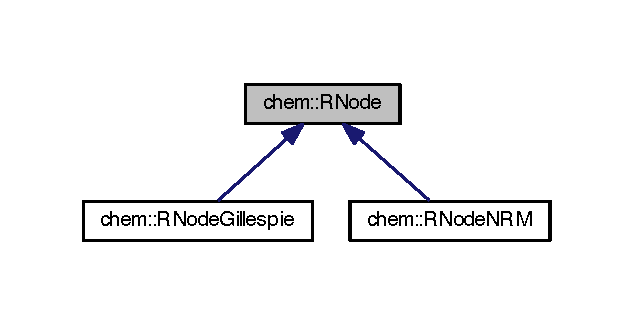
\includegraphics[width=312pt]{classchem_1_1RNode__inherit__graph}
\end{center}
\end{figure}
\subsection*{Public Member Functions}
\begin{DoxyCompactItemize}
\item 
virtual \hyperlink{classchem_1_1RNode_af39a9d08d697b5586dad42ce763b902d}{$\sim$\-R\-Node} ()
\begin{DoxyCompactList}\small\item\em Dtor. \end{DoxyCompactList}\item 
virtual void \hyperlink{classchem_1_1RNode_a979370f4102fdfda1ee562788318b556}{activate\-Reaction} ()=0
\begin{DoxyCompactList}\small\item\em This method is called by \hyperlink{classchem_1_1ReactionBase_aeb6c8f208d4c6ed1e0149090647eb035}{Reaction\-::activate\-Reaction()}. \end{DoxyCompactList}\item 
virtual void \hyperlink{classchem_1_1RNode_a007a65ede4d89e562929fc0ae9df5661}{passivate\-Reaction} ()=0
\begin{DoxyCompactList}\small\item\em This method is called by \hyperlink{classchem_1_1ReactionBase_a9fe4cf91fcff8c4aea65e759841c28fe}{Reaction\-::passivate\-Reaction()}. \end{DoxyCompactList}\item 
virtual bool \hyperlink{classchem_1_1RNode_a30bdb95406ebc217c1a732bf36883b3f}{is\-Passivated} () const =0
\begin{DoxyCompactList}\small\item\em Return true if the \hyperlink{classchem_1_1Reaction}{Reaction} is currently passivated. \end{DoxyCompactList}\end{DoxyCompactItemize}


\subsection{Detailed Description}
This is an abstract base class for classes that need to be associated with the given \hyperlink{classchem_1_1Reaction}{Reaction} object. 

Definition at line 15 of file Chem\-R\-Node.\-h.



\subsection{Constructor \& Destructor Documentation}
\hypertarget{classchem_1_1RNode_af39a9d08d697b5586dad42ce763b902d}{\index{chem\-::\-R\-Node@{chem\-::\-R\-Node}!$\sim$\-R\-Node@{$\sim$\-R\-Node}}
\index{$\sim$\-R\-Node@{$\sim$\-R\-Node}!chem::RNode@{chem\-::\-R\-Node}}
\subsubsection[{$\sim$\-R\-Node}]{\setlength{\rightskip}{0pt plus 5cm}virtual {\bf chem\-::\-R\-Node\-::$\sim$\-R\-Node} (
\begin{DoxyParamCaption}
{}
\end{DoxyParamCaption}
)\hspace{0.3cm}{\ttfamily  \mbox{[}inline, virtual\mbox{]}}}}\label{classchem_1_1RNode_af39a9d08d697b5586dad42ce763b902d}


Dtor. 



Definition at line 18 of file Chem\-R\-Node.\-h.



\subsection{Member Function Documentation}
\hypertarget{classchem_1_1RNode_a979370f4102fdfda1ee562788318b556}{\index{chem\-::\-R\-Node@{chem\-::\-R\-Node}!activate\-Reaction@{activate\-Reaction}}
\index{activate\-Reaction@{activate\-Reaction}!chem::RNode@{chem\-::\-R\-Node}}
\subsubsection[{activate\-Reaction}]{\setlength{\rightskip}{0pt plus 5cm}virtual void {\bf chem\-::\-R\-Node\-::activate\-Reaction} (
\begin{DoxyParamCaption}
{}
\end{DoxyParamCaption}
)\hspace{0.3cm}{\ttfamily  \mbox{[}pure virtual\mbox{]}}}}\label{classchem_1_1RNode_a979370f4102fdfda1ee562788318b556}


This method is called by \hyperlink{classchem_1_1ReactionBase_aeb6c8f208d4c6ed1e0149090647eb035}{Reaction\-::activate\-Reaction()}. 

Its effect depends on the underlying stochastic simulatio algorithm. For example, in the N\-R\-M algorithm, a new tau and a are computed and the heap is updated. 

Implemented in \hyperlink{classchem_1_1RNodeNRM_ae2fc1e8c09f0cda02da6cba29c6d0849}{chem\-::\-R\-Node\-N\-R\-M}, and \hyperlink{classchem_1_1RNodeGillespie_aefe90be75d811b0fa92234663c8d29ba}{chem\-::\-R\-Node\-Gillespie}.

\hypertarget{classchem_1_1RNode_a30bdb95406ebc217c1a732bf36883b3f}{\index{chem\-::\-R\-Node@{chem\-::\-R\-Node}!is\-Passivated@{is\-Passivated}}
\index{is\-Passivated@{is\-Passivated}!chem::RNode@{chem\-::\-R\-Node}}
\subsubsection[{is\-Passivated}]{\setlength{\rightskip}{0pt plus 5cm}virtual bool {\bf chem\-::\-R\-Node\-::is\-Passivated} (
\begin{DoxyParamCaption}
{}
\end{DoxyParamCaption}
) const\hspace{0.3cm}{\ttfamily  \mbox{[}pure virtual\mbox{]}}}}\label{classchem_1_1RNode_a30bdb95406ebc217c1a732bf36883b3f}


Return true if the \hyperlink{classchem_1_1Reaction}{Reaction} is currently passivated. 



Implemented in \hyperlink{classchem_1_1RNodeNRM_ad6445c86ef589c51c8d0957d437f6c3c}{chem\-::\-R\-Node\-N\-R\-M}, and \hyperlink{classchem_1_1RNodeGillespie_a456ac34c578988b02fc003d69ebc2d21}{chem\-::\-R\-Node\-Gillespie}.

\hypertarget{classchem_1_1RNode_a007a65ede4d89e562929fc0ae9df5661}{\index{chem\-::\-R\-Node@{chem\-::\-R\-Node}!passivate\-Reaction@{passivate\-Reaction}}
\index{passivate\-Reaction@{passivate\-Reaction}!chem::RNode@{chem\-::\-R\-Node}}
\subsubsection[{passivate\-Reaction}]{\setlength{\rightskip}{0pt plus 5cm}virtual void {\bf chem\-::\-R\-Node\-::passivate\-Reaction} (
\begin{DoxyParamCaption}
{}
\end{DoxyParamCaption}
)\hspace{0.3cm}{\ttfamily  \mbox{[}pure virtual\mbox{]}}}}\label{classchem_1_1RNode_a007a65ede4d89e562929fc0ae9df5661}


This method is called by \hyperlink{classchem_1_1ReactionBase_a9fe4cf91fcff8c4aea65e759841c28fe}{Reaction\-::passivate\-Reaction()}. 

Its effect depends on the underlying stochastic simulatio algorithm. For example, in the N\-R\-M algorithm, a tau is set to infinity and the heap is updated. 

Implemented in \hyperlink{classchem_1_1RNodeNRM_a1099526d4e797a6d033ad6f60b76dc12}{chem\-::\-R\-Node\-N\-R\-M}, and \hyperlink{classchem_1_1RNodeGillespie_a6b641601ec312a4169f07e2dcf797f41}{chem\-::\-R\-Node\-Gillespie}.



The documentation for this class was generated from the following file\-:\begin{DoxyCompactItemize}
\item 
Cyto\-Sim/\hyperlink{ChemRNode_8h}{Chem\-R\-Node.\-h}\end{DoxyCompactItemize}

\input{classchem_1_1RNodeGillespie}
\hypertarget{classchem_1_1RNodeNRM}{\section{chem\-:\-:R\-Node\-N\-R\-M Class Reference}
\label{classchem_1_1RNodeNRM}\index{chem\-::\-R\-Node\-N\-R\-M@{chem\-::\-R\-Node\-N\-R\-M}}
}


\hyperlink{classchem_1_1RNodeNRM}{R\-Node\-N\-R\-M} stands for \hyperlink{classchem_1_1Reaction}{Reaction} Node Next \hyperlink{classchem_1_1Reaction}{Reaction} Method.  




{\ttfamily \#include $<$Chem\-N\-R\-M\-Impl.\-h$>$}



Inheritance diagram for chem\-:\-:R\-Node\-N\-R\-M\-:\nopagebreak
\begin{figure}[H]
\begin{center}
\leavevmode
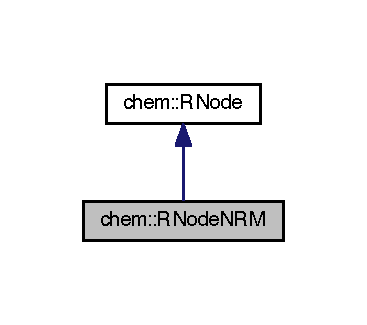
\includegraphics[width=178pt]{classchem_1_1RNodeNRM__inherit__graph}
\end{center}
\end{figure}


Collaboration diagram for chem\-:\-:R\-Node\-N\-R\-M\-:\nopagebreak
\begin{figure}[H]
\begin{center}
\leavevmode
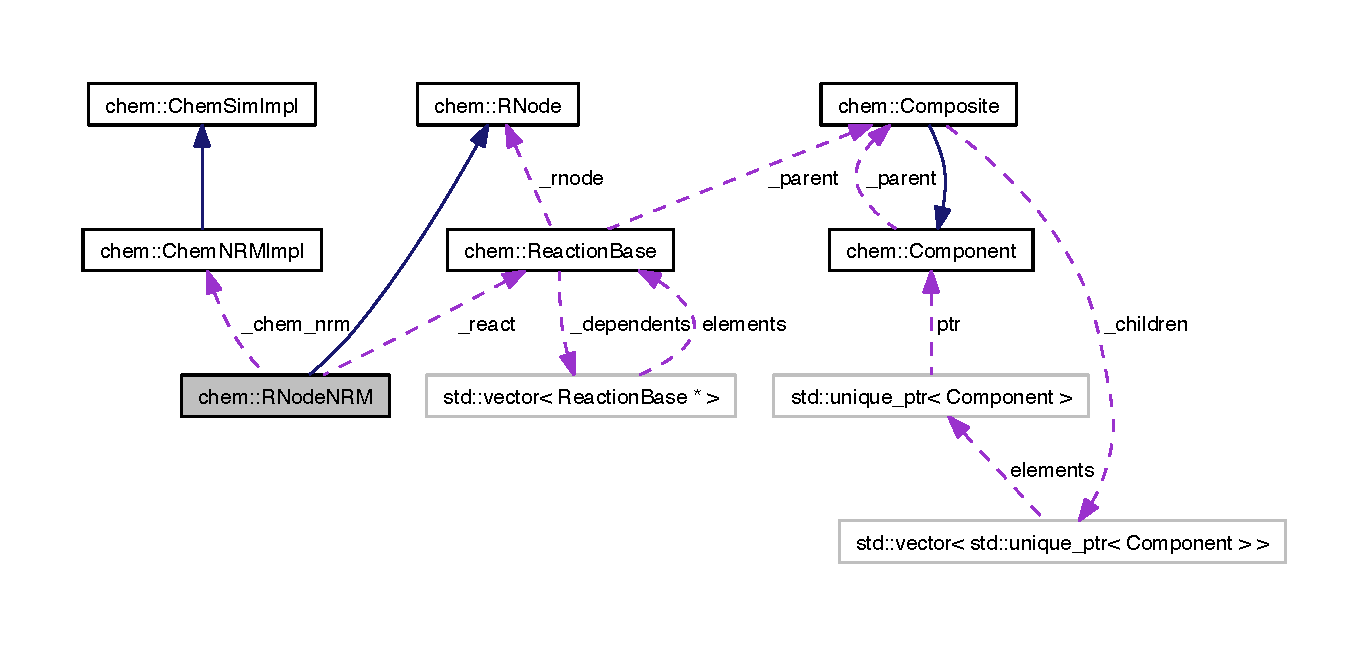
\includegraphics[width=350pt]{classchem_1_1RNodeNRM__coll__graph}
\end{center}
\end{figure}
\subsection*{Public Member Functions}
\begin{DoxyCompactItemize}
\item 
\hyperlink{classchem_1_1RNodeNRM_a4c5827a0d0682ecfbe7c9154ff5644ce}{R\-Node\-N\-R\-M} (\hyperlink{classchem_1_1ReactionBase}{Reaction\-Base} $\ast$r, \hyperlink{classchem_1_1ChemNRMImpl}{Chem\-N\-R\-M\-Impl} \&chem\-\_\-nrm)
\begin{DoxyCompactList}\small\item\em Ctor\-: \end{DoxyCompactList}\item 
\hyperlink{classchem_1_1RNodeNRM_a12d79f33bd69c1b58e18fa4de0d500df}{R\-Node\-N\-R\-M} (const \hyperlink{classchem_1_1RNodeNRM}{R\-Node\-N\-R\-M} \&rhs)
\begin{DoxyCompactList}\small\item\em Copying is not allowed. \end{DoxyCompactList}\item 
\hyperlink{classchem_1_1RNodeNRM}{R\-Node\-N\-R\-M} \& \hyperlink{classchem_1_1RNodeNRM_aba4753c700f2f6d707e2c94b2c5e5749}{operator=} (\hyperlink{classchem_1_1RNodeNRM}{R\-Node\-N\-R\-M} \&rhs)
\begin{DoxyCompactList}\small\item\em Assignment is not allowed. \end{DoxyCompactList}\item 
virtual \hyperlink{classchem_1_1RNodeNRM_ada0f6d009280070f3b89a22ab05c32a2}{$\sim$\-R\-Node\-N\-R\-M} ()
\begin{DoxyCompactList}\small\item\em Dtor\-: 1) Erases the corresponding \hyperlink{classchem_1_1PQNode}{P\-Q\-Node} element in the heap via the handle; 2) The \hyperlink{classchem_1_1RNode}{R\-Node} pointer of the tracked \hyperlink{classchem_1_1Reaction}{Reaction} object is set to nullptr. \end{DoxyCompactList}\item 
void \hyperlink{classchem_1_1RNodeNRM_a33025de761dc8d29928f8e5b1148eff1}{generate\-New\-Rand\-Tau} ()
\begin{DoxyCompactList}\small\item\em This methods recomputes the reaction propensity based on current coefficients and the rate, and then obtains a corresponding new tau drawn from an exponential distribution. \end{DoxyCompactList}\item 
\hyperlink{classchem_1_1ReactionBase}{Reaction\-Base} $\ast$ \hyperlink{classchem_1_1RNodeNRM_a8a96e9750901ff0629d43855ff096194}{get\-Reaction} () const 
\begin{DoxyCompactList}\small\item\em Returns a pointer to the \hyperlink{classchem_1_1Reaction}{Reaction} which corresponds to this \hyperlink{classchem_1_1RNodeNRM}{R\-Node\-N\-R\-M}. \end{DoxyCompactList}\item 
void \hyperlink{classchem_1_1RNodeNRM_a9de7334d3f16fc695929e97d9d296282}{update\-Heap} ()
\begin{DoxyCompactList}\small\item\em The heap is updated only with respect to the specific \hyperlink{classchem_1_1PQNode}{P\-Q\-Node} element which presumably was modified (e.\-g. \end{DoxyCompactList}\item 
double \hyperlink{classchem_1_1RNodeNRM_a570e4a825862fdf03d10e36fa186ba64}{get\-Tau} () const 
\begin{DoxyCompactList}\small\item\em Returns the tau from the the associated \hyperlink{classchem_1_1PQNode}{P\-Q\-Node} element. \end{DoxyCompactList}\item 
void \hyperlink{classchem_1_1RNodeNRM_aae070cd16c0acee98250c3d1bccd8fd0}{set\-Tau} (double \hyperlink{common_8h_abca55e6a21e0401c42bfb5da79ad3ad5}{tau})
\begin{DoxyCompactList}\small\item\em Sets the tau of the the associated \hyperlink{classchem_1_1PQNode}{P\-Q\-Node} element. Does not update the heap. \end{DoxyCompactList}\item 
\hyperlink{namespacechem_a33be80d87771bff54f5cede2e5d81cd1}{handle\-\_\-t} \& \hyperlink{classchem_1_1RNodeNRM_af5334e740100ba592f15abfe18b971a7}{get\-Handle} ()
\begin{DoxyCompactList}\small\item\em Returns a handle to the associated \hyperlink{classchem_1_1PQNode}{P\-Q\-Node} element, which can be used to access tau, for example. \end{DoxyCompactList}\item 
double \hyperlink{classchem_1_1RNodeNRM_a5894ae93a6ef48f7b0bfa82add5bce5d}{get\-Propensity} () const 
\begin{DoxyCompactList}\small\item\em Return the currently stored propensity, \char`\"{}a\char`\"{}, for this \hyperlink{classchem_1_1Reaction}{Reaction}. \end{DoxyCompactList}\item 
double \hyperlink{classchem_1_1RNodeNRM_adb047e14398dc54d6940158e408d504e}{re\-Compute\-Propensity} ()
\begin{DoxyCompactList}\small\item\em (Re)Compute and return the propensity associated with this \hyperlink{classchem_1_1Reaction}{Reaction}. \end{DoxyCompactList}\item 
int \hyperlink{classchem_1_1RNodeNRM_a1fd03a524da0a5ee5a63e9095b807bcf}{get\-Product\-Of\-Reactants} ()
\begin{DoxyCompactList}\small\item\em Compute and return the product of reactant copy numbers. \end{DoxyCompactList}\item 
void \hyperlink{classchem_1_1RNodeNRM_a1294bf93224e88f4bb0a64282ef9f950}{make\-Step} ()
\begin{DoxyCompactList}\small\item\em This method calls the corresponding \hyperlink{classchem_1_1ReactionBase_acb5575b08ca39fc6dd7a571fb246806b}{Reaction\-::make\-Step()} method of the underyling \hyperlink{classchem_1_1Reaction}{Reaction} object. \end{DoxyCompactList}\item 
virtual void \hyperlink{classchem_1_1RNodeNRM_ae2fc1e8c09f0cda02da6cba29c6d0849}{activate\-Reaction} ()
\begin{DoxyCompactList}\small\item\em When this method is called, a new tau is computed and the corresponding \hyperlink{classchem_1_1PQNode}{P\-Q\-Node} element is updated in the heap. \end{DoxyCompactList}\item 
virtual void \hyperlink{classchem_1_1RNodeNRM_a1099526d4e797a6d033ad6f60b76dc12}{passivate\-Reaction} ()
\begin{DoxyCompactList}\small\item\em When this method is called, reaction's tau is set to infinity, the propensity is set to 0, and the corresponding \hyperlink{classchem_1_1PQNode}{P\-Q\-Node} element is updated in the heap. \end{DoxyCompactList}\item 
bool \hyperlink{classchem_1_1RNodeNRM_ad6445c86ef589c51c8d0957d437f6c3c}{is\-Passivated} () const 
\begin{DoxyCompactList}\small\item\em Return true if the \hyperlink{classchem_1_1Reaction}{Reaction} is currently passivated. \end{DoxyCompactList}\item 
void \hyperlink{classchem_1_1RNodeNRM_a1855b936b240d7764907434421258c5a}{print\-Self} () const 
\begin{DoxyCompactList}\small\item\em Print information about this \hyperlink{classchem_1_1RNodeNRM}{R\-Node\-N\-R\-M} such as tau, a and the \hyperlink{classchem_1_1Reaction}{Reaction} which this \hyperlink{classchem_1_1RNodeNRM}{R\-Node\-N\-R\-M} tracks. \end{DoxyCompactList}\item 
void \hyperlink{classchem_1_1RNodeNRM_ad8e5f9557c3ba701596aff928dc5270e}{print\-Dependents} () const 
\begin{DoxyCompactList}\small\item\em Print the \hyperlink{classchem_1_1RNode}{R\-Node} objects which are dependents of this \hyperlink{classchem_1_1RNode}{R\-Node} (via the tracked \hyperlink{classchem_1_1Reaction}{Reaction} object dependencies) \end{DoxyCompactList}\end{DoxyCompactItemize}
\subsection*{Private Attributes}
\begin{DoxyCompactItemize}
\item 
\hyperlink{classchem_1_1ChemNRMImpl}{Chem\-N\-R\-M\-Impl} \& \hyperlink{classchem_1_1RNodeNRM_acff43a1b27a778b6534bd8010904f821}{\-\_\-chem\-\_\-nrm}
\begin{DoxyCompactList}\small\item\em A reference to the \hyperlink{classchem_1_1ChemNRMImpl}{Chem\-N\-R\-M\-Impl} which containts the heap, random number generators, etc. \end{DoxyCompactList}\item 
\hyperlink{namespacechem_a33be80d87771bff54f5cede2e5d81cd1}{handle\-\_\-t} \hyperlink{classchem_1_1RNodeNRM_ad124c85b0f1b479cf0c1f4bf75230c19}{\-\_\-handle}
\begin{DoxyCompactList}\small\item\em The handle to the associated \hyperlink{classchem_1_1PQNode}{P\-Q\-Node} element in the heap. \end{DoxyCompactList}\item 
\hyperlink{classchem_1_1ReactionBase}{Reaction\-Base} $\ast$ \hyperlink{classchem_1_1RNodeNRM_add823fa4b223afe0d750ed731c827d07}{\-\_\-react}
\begin{DoxyCompactList}\small\item\em The pointer to the associated \hyperlink{classchem_1_1Reaction}{Reaction} object. The corresponding memory is not managed by \hyperlink{classchem_1_1RNodeNRM}{R\-Node\-N\-R\-M}. \end{DoxyCompactList}\item 
double \hyperlink{classchem_1_1RNodeNRM_ae16aa8e75649d855f4b6eae8b00ed1db}{\-\_\-a}
\begin{DoxyCompactList}\small\item\em The propensity associated with the \hyperlink{classchem_1_1Reaction}{Reaction}. It may be outdated and may need to be recomputed if needed. \end{DoxyCompactList}\end{DoxyCompactItemize}


\subsection{Detailed Description}
\hyperlink{classchem_1_1RNodeNRM}{R\-Node\-N\-R\-M} stands for \hyperlink{classchem_1_1Reaction}{Reaction} Node Next \hyperlink{classchem_1_1Reaction}{Reaction} Method. 

\hyperlink{classchem_1_1RNodeNRM}{R\-Node\-N\-R\-M} manages a single chemical reaction within the N\-R\-M algorithm. It has a pointer to the P\-Q element containing the \hyperlink{classchem_1_1Reaction}{Reaction} via a handle\-\_\-t object (and hence can modify both the corresponding \hyperlink{classchem_1_1PQNode}{P\-Q\-Node}, such as \hyperlink{classchem_1_1PQNode}{P\-Q\-Node}'s tau or the underlying \hyperlink{classchem_1_1Reaction}{Reaction} instance). \hyperlink{classchem_1_1RNodeNRM}{R\-Node\-N\-R\-M} can recompute tau if needed and has auxiliary methods for computing reaction's propensity. When the propensity drops to zero, the \hyperlink{classchem_1_1RNodeNRM}{R\-Node\-N\-R\-M} can execute the \hyperlink{classchem_1_1RNodeNRM_a1099526d4e797a6d033ad6f60b76dc12}{passivate\-Reaction()} method. Alternatively, passivated \hyperlink{classchem_1_1RNodeNRM}{R\-Node\-N\-R\-M} can be activated via \hyperlink{classchem_1_1RNodeNRM_ae2fc1e8c09f0cda02da6cba29c6d0849}{activate\-Reaction()}. The main part of the N\-R\-M algoritm is implemented in the \hyperlink{classchem_1_1RNodeNRM_a1294bf93224e88f4bb0a64282ef9f950}{make\-Step()} method. 

Definition at line 103 of file Chem\-N\-R\-M\-Impl.\-h.



\subsection{Constructor \& Destructor Documentation}
\hypertarget{classchem_1_1RNodeNRM_a4c5827a0d0682ecfbe7c9154ff5644ce}{\index{chem\-::\-R\-Node\-N\-R\-M@{chem\-::\-R\-Node\-N\-R\-M}!R\-Node\-N\-R\-M@{R\-Node\-N\-R\-M}}
\index{R\-Node\-N\-R\-M@{R\-Node\-N\-R\-M}!chem::RNodeNRM@{chem\-::\-R\-Node\-N\-R\-M}}
\subsubsection[{R\-Node\-N\-R\-M}]{\setlength{\rightskip}{0pt plus 5cm}{\bf chem\-::\-R\-Node\-N\-R\-M\-::\-R\-Node\-N\-R\-M} (
\begin{DoxyParamCaption}
\item[{{\bf Reaction\-Base} $\ast$}]{r, }
\item[{{\bf Chem\-N\-R\-M\-Impl} \&}]{chem\-\_\-nrm}
\end{DoxyParamCaption}
)}}\label{classchem_1_1RNodeNRM_a4c5827a0d0682ecfbe7c9154ff5644ce}


Ctor\-: 


\begin{DoxyParams}{Parameters}
{\em $\ast$r} & is the \hyperlink{classchem_1_1Reaction}{Reaction} object corresponding to this \hyperlink{classchem_1_1RNodeNRM}{R\-Node\-N\-R\-M} \\
\hline
{\em \&chem\-\_\-nrm} & is a refernce to \hyperlink{classchem_1_1ChemNRMImpl}{Chem\-N\-R\-M\-Impl} object, which does the overall management of the N\-R\-M scheme (e.\-g. it gives acces to the heap itself, random distribution generators, etc.) \\
\hline
\end{DoxyParams}


Definition at line 79 of file Chem\-N\-R\-M\-Impl.\-cpp.



References \-\_\-a, \-\_\-chem\-\_\-nrm, \-\_\-handle, \-\_\-react, chem\-::\-Reaction\-Base\-::compute\-Propensity(), chem\-::\-Chem\-N\-R\-M\-Impl\-::get\-Heap(), and chem\-::\-Reaction\-Base\-::set\-Rnode().

\hypertarget{classchem_1_1RNodeNRM_a12d79f33bd69c1b58e18fa4de0d500df}{\index{chem\-::\-R\-Node\-N\-R\-M@{chem\-::\-R\-Node\-N\-R\-M}!R\-Node\-N\-R\-M@{R\-Node\-N\-R\-M}}
\index{R\-Node\-N\-R\-M@{R\-Node\-N\-R\-M}!chem::RNodeNRM@{chem\-::\-R\-Node\-N\-R\-M}}
\subsubsection[{R\-Node\-N\-R\-M}]{\setlength{\rightskip}{0pt plus 5cm}{\bf chem\-::\-R\-Node\-N\-R\-M\-::\-R\-Node\-N\-R\-M} (
\begin{DoxyParamCaption}
\item[{const {\bf R\-Node\-N\-R\-M} \&}]{rhs}
\end{DoxyParamCaption}
)}}\label{classchem_1_1RNodeNRM_a12d79f33bd69c1b58e18fa4de0d500df}


Copying is not allowed. 

\hypertarget{classchem_1_1RNodeNRM_ada0f6d009280070f3b89a22ab05c32a2}{\index{chem\-::\-R\-Node\-N\-R\-M@{chem\-::\-R\-Node\-N\-R\-M}!$\sim$\-R\-Node\-N\-R\-M@{$\sim$\-R\-Node\-N\-R\-M}}
\index{$\sim$\-R\-Node\-N\-R\-M@{$\sim$\-R\-Node\-N\-R\-M}!chem::RNodeNRM@{chem\-::\-R\-Node\-N\-R\-M}}
\subsubsection[{$\sim$\-R\-Node\-N\-R\-M}]{\setlength{\rightskip}{0pt plus 5cm}{\bf chem\-::\-R\-Node\-N\-R\-M\-::$\sim$\-R\-Node\-N\-R\-M} (
\begin{DoxyParamCaption}
{}
\end{DoxyParamCaption}
)\hspace{0.3cm}{\ttfamily  \mbox{[}virtual\mbox{]}}}}\label{classchem_1_1RNodeNRM_ada0f6d009280070f3b89a22ab05c32a2}


Dtor\-: 1) Erases the corresponding \hyperlink{classchem_1_1PQNode}{P\-Q\-Node} element in the heap via the handle; 2) The \hyperlink{classchem_1_1RNode}{R\-Node} pointer of the tracked \hyperlink{classchem_1_1Reaction}{Reaction} object is set to nullptr. 



Definition at line 87 of file Chem\-N\-R\-M\-Impl.\-cpp.



References \-\_\-chem\-\_\-nrm, \-\_\-handle, \-\_\-react, chem\-::\-Chem\-N\-R\-M\-Impl\-::get\-Heap(), and chem\-::\-Reaction\-Base\-::set\-Rnode().



\subsection{Member Function Documentation}
\hypertarget{classchem_1_1RNodeNRM_ae2fc1e8c09f0cda02da6cba29c6d0849}{\index{chem\-::\-R\-Node\-N\-R\-M@{chem\-::\-R\-Node\-N\-R\-M}!activate\-Reaction@{activate\-Reaction}}
\index{activate\-Reaction@{activate\-Reaction}!chem::RNodeNRM@{chem\-::\-R\-Node\-N\-R\-M}}
\subsubsection[{activate\-Reaction}]{\setlength{\rightskip}{0pt plus 5cm}void {\bf chem\-::\-R\-Node\-N\-R\-M\-::activate\-Reaction} (
\begin{DoxyParamCaption}
{}
\end{DoxyParamCaption}
)\hspace{0.3cm}{\ttfamily  \mbox{[}virtual\mbox{]}}}}\label{classchem_1_1RNodeNRM_ae2fc1e8c09f0cda02da6cba29c6d0849}


When this method is called, a new tau is computed and the corresponding \hyperlink{classchem_1_1PQNode}{P\-Q\-Node} element is updated in the heap. 

\begin{DoxyNote}{Note}
This method does not activate the \hyperlink{classchem_1_1Reaction}{Reaction} itself, but instead only deals with the activation process related to the corresponding \hyperlink{classchem_1_1PQNode}{P\-Q\-Node} element. 
\end{DoxyNote}


Implements \hyperlink{classchem_1_1RNode_a979370f4102fdfda1ee562788318b556}{chem\-::\-R\-Node}.



Definition at line 132 of file Chem\-N\-R\-M\-Impl.\-cpp.



References generate\-New\-Rand\-Tau(), and update\-Heap().

\hypertarget{classchem_1_1RNodeNRM_a33025de761dc8d29928f8e5b1148eff1}{\index{chem\-::\-R\-Node\-N\-R\-M@{chem\-::\-R\-Node\-N\-R\-M}!generate\-New\-Rand\-Tau@{generate\-New\-Rand\-Tau}}
\index{generate\-New\-Rand\-Tau@{generate\-New\-Rand\-Tau}!chem::RNodeNRM@{chem\-::\-R\-Node\-N\-R\-M}}
\subsubsection[{generate\-New\-Rand\-Tau}]{\setlength{\rightskip}{0pt plus 5cm}void {\bf chem\-::\-R\-Node\-N\-R\-M\-::generate\-New\-Rand\-Tau} (
\begin{DoxyParamCaption}
{}
\end{DoxyParamCaption}
)}}\label{classchem_1_1RNodeNRM_a33025de761dc8d29928f8e5b1148eff1}


This methods recomputes the reaction propensity based on current coefficients and the rate, and then obtains a corresponding new tau drawn from an exponential distribution. 

\begin{DoxyNote}{Note}
This methods modifies tau which is stored in the associated \hyperlink{classchem_1_1PQNode}{P\-Q\-Node} object. However, it does not update the heap -\/ this needs to be done seprately. 
\end{DoxyNote}


Definition at line 116 of file Chem\-N\-R\-M\-Impl.\-cpp.



References \-\_\-a, \-\_\-chem\-\_\-nrm, chem\-::\-Chem\-N\-R\-M\-Impl\-::generate\-Tau(), chem\-::\-Chem\-N\-R\-M\-Impl\-::get\-Time(), re\-Compute\-Propensity(), set\-Tau(), and tau().



Referenced by activate\-Reaction(), and chem\-::\-Chem\-N\-R\-M\-Impl\-::make\-Step().

\hypertarget{classchem_1_1RNodeNRM_af5334e740100ba592f15abfe18b971a7}{\index{chem\-::\-R\-Node\-N\-R\-M@{chem\-::\-R\-Node\-N\-R\-M}!get\-Handle@{get\-Handle}}
\index{get\-Handle@{get\-Handle}!chem::RNodeNRM@{chem\-::\-R\-Node\-N\-R\-M}}
\subsubsection[{get\-Handle}]{\setlength{\rightskip}{0pt plus 5cm}{\bf handle\-\_\-t}\& {\bf chem\-::\-R\-Node\-N\-R\-M\-::get\-Handle} (
\begin{DoxyParamCaption}
{}
\end{DoxyParamCaption}
)\hspace{0.3cm}{\ttfamily  \mbox{[}inline\mbox{]}}}}\label{classchem_1_1RNodeNRM_af5334e740100ba592f15abfe18b971a7}


Returns a handle to the associated \hyperlink{classchem_1_1PQNode}{P\-Q\-Node} element, which can be used to access tau, for example. 



Definition at line 141 of file Chem\-N\-R\-M\-Impl.\-h.



References \-\_\-handle.

\hypertarget{classchem_1_1RNodeNRM_a1fd03a524da0a5ee5a63e9095b807bcf}{\index{chem\-::\-R\-Node\-N\-R\-M@{chem\-::\-R\-Node\-N\-R\-M}!get\-Product\-Of\-Reactants@{get\-Product\-Of\-Reactants}}
\index{get\-Product\-Of\-Reactants@{get\-Product\-Of\-Reactants}!chem::RNodeNRM@{chem\-::\-R\-Node\-N\-R\-M}}
\subsubsection[{get\-Product\-Of\-Reactants}]{\setlength{\rightskip}{0pt plus 5cm}int {\bf chem\-::\-R\-Node\-N\-R\-M\-::get\-Product\-Of\-Reactants} (
\begin{DoxyParamCaption}
{}
\end{DoxyParamCaption}
)\hspace{0.3cm}{\ttfamily  \mbox{[}inline\mbox{]}}}}\label{classchem_1_1RNodeNRM_a1fd03a524da0a5ee5a63e9095b807bcf}


Compute and return the product of reactant copy numbers. 

This method can be used to quickly check whether this reaction needs to be passivated, if the returned result is zero. 

Definition at line 152 of file Chem\-N\-R\-M\-Impl.\-h.



References \-\_\-react, and chem\-::\-Reaction\-Base\-::get\-Product\-Of\-Reactants().

\hypertarget{classchem_1_1RNodeNRM_a5894ae93a6ef48f7b0bfa82add5bce5d}{\index{chem\-::\-R\-Node\-N\-R\-M@{chem\-::\-R\-Node\-N\-R\-M}!get\-Propensity@{get\-Propensity}}
\index{get\-Propensity@{get\-Propensity}!chem::RNodeNRM@{chem\-::\-R\-Node\-N\-R\-M}}
\subsubsection[{get\-Propensity}]{\setlength{\rightskip}{0pt plus 5cm}double {\bf chem\-::\-R\-Node\-N\-R\-M\-::get\-Propensity} (
\begin{DoxyParamCaption}
{}
\end{DoxyParamCaption}
) const\hspace{0.3cm}{\ttfamily  \mbox{[}inline\mbox{]}}}}\label{classchem_1_1RNodeNRM_a5894ae93a6ef48f7b0bfa82add5bce5d}


Return the currently stored propensity, \char`\"{}a\char`\"{}, for this \hyperlink{classchem_1_1Reaction}{Reaction}. 

\begin{DoxyNote}{Note}
The propensity is not recomputed in this method, so it potentially can be out of sync. 
\end{DoxyNote}


Definition at line 145 of file Chem\-N\-R\-M\-Impl.\-h.



References \-\_\-a.



Referenced by chem\-::\-Chem\-N\-R\-M\-Impl\-::make\-Step().

\hypertarget{classchem_1_1RNodeNRM_a8a96e9750901ff0629d43855ff096194}{\index{chem\-::\-R\-Node\-N\-R\-M@{chem\-::\-R\-Node\-N\-R\-M}!get\-Reaction@{get\-Reaction}}
\index{get\-Reaction@{get\-Reaction}!chem::RNodeNRM@{chem\-::\-R\-Node\-N\-R\-M}}
\subsubsection[{get\-Reaction}]{\setlength{\rightskip}{0pt plus 5cm}{\bf Reaction\-Base}$\ast$ {\bf chem\-::\-R\-Node\-N\-R\-M\-::get\-Reaction} (
\begin{DoxyParamCaption}
{}
\end{DoxyParamCaption}
) const\hspace{0.3cm}{\ttfamily  \mbox{[}inline\mbox{]}}}}\label{classchem_1_1RNodeNRM_a8a96e9750901ff0629d43855ff096194}


Returns a pointer to the \hyperlink{classchem_1_1Reaction}{Reaction} which corresponds to this \hyperlink{classchem_1_1RNodeNRM}{R\-Node\-N\-R\-M}. 



Definition at line 128 of file Chem\-N\-R\-M\-Impl.\-h.



References \-\_\-react.



Referenced by chem\-::\-Chem\-N\-R\-M\-Impl\-::make\-Step().

\hypertarget{classchem_1_1RNodeNRM_a570e4a825862fdf03d10e36fa186ba64}{\index{chem\-::\-R\-Node\-N\-R\-M@{chem\-::\-R\-Node\-N\-R\-M}!get\-Tau@{get\-Tau}}
\index{get\-Tau@{get\-Tau}!chem::RNodeNRM@{chem\-::\-R\-Node\-N\-R\-M}}
\subsubsection[{get\-Tau}]{\setlength{\rightskip}{0pt plus 5cm}double {\bf chem\-::\-R\-Node\-N\-R\-M\-::get\-Tau} (
\begin{DoxyParamCaption}
{}
\end{DoxyParamCaption}
) const\hspace{0.3cm}{\ttfamily  \mbox{[}inline\mbox{]}}}}\label{classchem_1_1RNodeNRM_a570e4a825862fdf03d10e36fa186ba64}


Returns the tau from the the associated \hyperlink{classchem_1_1PQNode}{P\-Q\-Node} element. 



Definition at line 135 of file Chem\-N\-R\-M\-Impl.\-h.



Referenced by chem\-::\-Chem\-N\-R\-M\-Impl\-::make\-Step(), and print\-Self().

\hypertarget{classchem_1_1RNodeNRM_ad6445c86ef589c51c8d0957d437f6c3c}{\index{chem\-::\-R\-Node\-N\-R\-M@{chem\-::\-R\-Node\-N\-R\-M}!is\-Passivated@{is\-Passivated}}
\index{is\-Passivated@{is\-Passivated}!chem::RNodeNRM@{chem\-::\-R\-Node\-N\-R\-M}}
\subsubsection[{is\-Passivated}]{\setlength{\rightskip}{0pt plus 5cm}bool {\bf chem\-::\-R\-Node\-N\-R\-M\-::is\-Passivated} (
\begin{DoxyParamCaption}
{}
\end{DoxyParamCaption}
) const\hspace{0.3cm}{\ttfamily  \mbox{[}inline, virtual\mbox{]}}}}\label{classchem_1_1RNodeNRM_ad6445c86ef589c51c8d0957d437f6c3c}


Return true if the \hyperlink{classchem_1_1Reaction}{Reaction} is currently passivated. 



Implements \hyperlink{classchem_1_1RNode_a30bdb95406ebc217c1a732bf36883b3f}{chem\-::\-R\-Node}.



Definition at line 169 of file Chem\-N\-R\-M\-Impl.\-h.



References \-\_\-react, and chem\-::\-Reaction\-Base\-::is\-Passivated().



Referenced by chem\-::\-Chem\-N\-R\-M\-Impl\-::make\-Step().

\hypertarget{classchem_1_1RNodeNRM_a1294bf93224e88f4bb0a64282ef9f950}{\index{chem\-::\-R\-Node\-N\-R\-M@{chem\-::\-R\-Node\-N\-R\-M}!make\-Step@{make\-Step}}
\index{make\-Step@{make\-Step}!chem::RNodeNRM@{chem\-::\-R\-Node\-N\-R\-M}}
\subsubsection[{make\-Step}]{\setlength{\rightskip}{0pt plus 5cm}void {\bf chem\-::\-R\-Node\-N\-R\-M\-::make\-Step} (
\begin{DoxyParamCaption}
{}
\end{DoxyParamCaption}
)\hspace{0.3cm}{\ttfamily  \mbox{[}inline\mbox{]}}}}\label{classchem_1_1RNodeNRM_a1294bf93224e88f4bb0a64282ef9f950}


This method calls the corresponding \hyperlink{classchem_1_1ReactionBase_acb5575b08ca39fc6dd7a571fb246806b}{Reaction\-::make\-Step()} method of the underyling \hyperlink{classchem_1_1Reaction}{Reaction} object. 



Definition at line 155 of file Chem\-N\-R\-M\-Impl.\-h.



References \-\_\-react, and chem\-::\-Reaction\-Base\-::make\-Step().



Referenced by chem\-::\-Chem\-N\-R\-M\-Impl\-::make\-Step().

\hypertarget{classchem_1_1RNodeNRM_aba4753c700f2f6d707e2c94b2c5e5749}{\index{chem\-::\-R\-Node\-N\-R\-M@{chem\-::\-R\-Node\-N\-R\-M}!operator=@{operator=}}
\index{operator=@{operator=}!chem::RNodeNRM@{chem\-::\-R\-Node\-N\-R\-M}}
\subsubsection[{operator=}]{\setlength{\rightskip}{0pt plus 5cm}{\bf R\-Node\-N\-R\-M}\& chem\-::\-R\-Node\-N\-R\-M\-::operator= (
\begin{DoxyParamCaption}
\item[{{\bf R\-Node\-N\-R\-M} \&}]{rhs}
\end{DoxyParamCaption}
)}}\label{classchem_1_1RNodeNRM_aba4753c700f2f6d707e2c94b2c5e5749}


Assignment is not allowed. 

\hypertarget{classchem_1_1RNodeNRM_a1099526d4e797a6d033ad6f60b76dc12}{\index{chem\-::\-R\-Node\-N\-R\-M@{chem\-::\-R\-Node\-N\-R\-M}!passivate\-Reaction@{passivate\-Reaction}}
\index{passivate\-Reaction@{passivate\-Reaction}!chem::RNodeNRM@{chem\-::\-R\-Node\-N\-R\-M}}
\subsubsection[{passivate\-Reaction}]{\setlength{\rightskip}{0pt plus 5cm}void {\bf chem\-::\-R\-Node\-N\-R\-M\-::passivate\-Reaction} (
\begin{DoxyParamCaption}
{}
\end{DoxyParamCaption}
)\hspace{0.3cm}{\ttfamily  \mbox{[}virtual\mbox{]}}}}\label{classchem_1_1RNodeNRM_a1099526d4e797a6d033ad6f60b76dc12}


When this method is called, reaction's tau is set to infinity, the propensity is set to 0, and the corresponding \hyperlink{classchem_1_1PQNode}{P\-Q\-Node} element is updated in the heap. 

\begin{DoxyNote}{Note}
This method does not passivate the \hyperlink{classchem_1_1Reaction}{Reaction} itself, but instead only deals with the activation process related to the corresponding \hyperlink{classchem_1_1PQNode}{P\-Q\-Node} element. 
\end{DoxyNote}


Implements \hyperlink{classchem_1_1RNode_a007a65ede4d89e562929fc0ae9df5661}{chem\-::\-R\-Node}.



Definition at line 141 of file Chem\-N\-R\-M\-Impl.\-cpp.



References \-\_\-a, set\-Tau(), tau(), and update\-Heap().

\hypertarget{classchem_1_1RNodeNRM_ad8e5f9557c3ba701596aff928dc5270e}{\index{chem\-::\-R\-Node\-N\-R\-M@{chem\-::\-R\-Node\-N\-R\-M}!print\-Dependents@{print\-Dependents}}
\index{print\-Dependents@{print\-Dependents}!chem::RNodeNRM@{chem\-::\-R\-Node\-N\-R\-M}}
\subsubsection[{print\-Dependents}]{\setlength{\rightskip}{0pt plus 5cm}void {\bf chem\-::\-R\-Node\-N\-R\-M\-::print\-Dependents} (
\begin{DoxyParamCaption}
{}
\end{DoxyParamCaption}
) const}}\label{classchem_1_1RNodeNRM_ad8e5f9557c3ba701596aff928dc5270e}


Print the \hyperlink{classchem_1_1RNode}{R\-Node} objects which are dependents of this \hyperlink{classchem_1_1RNode}{R\-Node} (via the tracked \hyperlink{classchem_1_1Reaction}{Reaction} object dependencies) 



Definition at line 101 of file Chem\-N\-R\-M\-Impl.\-cpp.



References \-\_\-react, chem\-::\-Reaction\-Base\-::dependents(), and print\-Self().

\hypertarget{classchem_1_1RNodeNRM_a1855b936b240d7764907434421258c5a}{\index{chem\-::\-R\-Node\-N\-R\-M@{chem\-::\-R\-Node\-N\-R\-M}!print\-Self@{print\-Self}}
\index{print\-Self@{print\-Self}!chem::RNodeNRM@{chem\-::\-R\-Node\-N\-R\-M}}
\subsubsection[{print\-Self}]{\setlength{\rightskip}{0pt plus 5cm}void {\bf chem\-::\-R\-Node\-N\-R\-M\-::print\-Self} (
\begin{DoxyParamCaption}
{}
\end{DoxyParamCaption}
) const}}\label{classchem_1_1RNodeNRM_a1855b936b240d7764907434421258c5a}


Print information about this \hyperlink{classchem_1_1RNodeNRM}{R\-Node\-N\-R\-M} such as tau, a and the \hyperlink{classchem_1_1Reaction}{Reaction} which this \hyperlink{classchem_1_1RNodeNRM}{R\-Node\-N\-R\-M} tracks. 



Definition at line 96 of file Chem\-N\-R\-M\-Impl.\-cpp.



References \-\_\-a, and get\-Tau().



Referenced by print\-Dependents().

\hypertarget{classchem_1_1RNodeNRM_adb047e14398dc54d6940158e408d504e}{\index{chem\-::\-R\-Node\-N\-R\-M@{chem\-::\-R\-Node\-N\-R\-M}!re\-Compute\-Propensity@{re\-Compute\-Propensity}}
\index{re\-Compute\-Propensity@{re\-Compute\-Propensity}!chem::RNodeNRM@{chem\-::\-R\-Node\-N\-R\-M}}
\subsubsection[{re\-Compute\-Propensity}]{\setlength{\rightskip}{0pt plus 5cm}double {\bf chem\-::\-R\-Node\-N\-R\-M\-::re\-Compute\-Propensity} (
\begin{DoxyParamCaption}
{}
\end{DoxyParamCaption}
)\hspace{0.3cm}{\ttfamily  \mbox{[}inline\mbox{]}}}}\label{classchem_1_1RNodeNRM_adb047e14398dc54d6940158e408d504e}


(Re)Compute and return the propensity associated with this \hyperlink{classchem_1_1Reaction}{Reaction}. 



Definition at line 148 of file Chem\-N\-R\-M\-Impl.\-h.



References \-\_\-a, \-\_\-react, and chem\-::\-Reaction\-Base\-::compute\-Propensity().



Referenced by generate\-New\-Rand\-Tau(), and chem\-::\-Chem\-N\-R\-M\-Impl\-::make\-Step().

\hypertarget{classchem_1_1RNodeNRM_aae070cd16c0acee98250c3d1bccd8fd0}{\index{chem\-::\-R\-Node\-N\-R\-M@{chem\-::\-R\-Node\-N\-R\-M}!set\-Tau@{set\-Tau}}
\index{set\-Tau@{set\-Tau}!chem::RNodeNRM@{chem\-::\-R\-Node\-N\-R\-M}}
\subsubsection[{set\-Tau}]{\setlength{\rightskip}{0pt plus 5cm}void {\bf chem\-::\-R\-Node\-N\-R\-M\-::set\-Tau} (
\begin{DoxyParamCaption}
\item[{double}]{tau}
\end{DoxyParamCaption}
)\hspace{0.3cm}{\ttfamily  \mbox{[}inline\mbox{]}}}}\label{classchem_1_1RNodeNRM_aae070cd16c0acee98250c3d1bccd8fd0}


Sets the tau of the the associated \hyperlink{classchem_1_1PQNode}{P\-Q\-Node} element. Does not update the heap. 



Definition at line 138 of file Chem\-N\-R\-M\-Impl.\-h.



References tau().



Referenced by generate\-New\-Rand\-Tau(), chem\-::\-Chem\-N\-R\-M\-Impl\-::make\-Step(), and passivate\-Reaction().

\hypertarget{classchem_1_1RNodeNRM_a9de7334d3f16fc695929e97d9d296282}{\index{chem\-::\-R\-Node\-N\-R\-M@{chem\-::\-R\-Node\-N\-R\-M}!update\-Heap@{update\-Heap}}
\index{update\-Heap@{update\-Heap}!chem::RNodeNRM@{chem\-::\-R\-Node\-N\-R\-M}}
\subsubsection[{update\-Heap}]{\setlength{\rightskip}{0pt plus 5cm}void {\bf chem\-::\-R\-Node\-N\-R\-M\-::update\-Heap} (
\begin{DoxyParamCaption}
{}
\end{DoxyParamCaption}
)}}\label{classchem_1_1RNodeNRM_a9de7334d3f16fc695929e97d9d296282}


The heap is updated only with respect to the specific \hyperlink{classchem_1_1PQNode}{P\-Q\-Node} element which presumably was modified (e.\-g. 

via \hyperlink{classchem_1_1RNodeNRM_a33025de761dc8d29928f8e5b1148eff1}{generate\-New\-Rand\-Tau()}). 

Definition at line 111 of file Chem\-N\-R\-M\-Impl.\-cpp.



References \-\_\-chem\-\_\-nrm, \-\_\-handle, and chem\-::\-Chem\-N\-R\-M\-Impl\-::get\-Heap().



Referenced by activate\-Reaction(), chem\-::\-Chem\-N\-R\-M\-Impl\-::make\-Step(), and passivate\-Reaction().



\subsection{Member Data Documentation}
\hypertarget{classchem_1_1RNodeNRM_ae16aa8e75649d855f4b6eae8b00ed1db}{\index{chem\-::\-R\-Node\-N\-R\-M@{chem\-::\-R\-Node\-N\-R\-M}!\-\_\-a@{\-\_\-a}}
\index{\-\_\-a@{\-\_\-a}!chem::RNodeNRM@{chem\-::\-R\-Node\-N\-R\-M}}
\subsubsection[{\-\_\-a}]{\setlength{\rightskip}{0pt plus 5cm}double {\bf chem\-::\-R\-Node\-N\-R\-M\-::\-\_\-a}\hspace{0.3cm}{\ttfamily  \mbox{[}private\mbox{]}}}}\label{classchem_1_1RNodeNRM_ae16aa8e75649d855f4b6eae8b00ed1db}


The propensity associated with the \hyperlink{classchem_1_1Reaction}{Reaction}. It may be outdated and may need to be recomputed if needed. 



Definition at line 189 of file Chem\-N\-R\-M\-Impl.\-h.



Referenced by generate\-New\-Rand\-Tau(), get\-Propensity(), passivate\-Reaction(), print\-Self(), re\-Compute\-Propensity(), and R\-Node\-N\-R\-M().

\hypertarget{classchem_1_1RNodeNRM_acff43a1b27a778b6534bd8010904f821}{\index{chem\-::\-R\-Node\-N\-R\-M@{chem\-::\-R\-Node\-N\-R\-M}!\-\_\-chem\-\_\-nrm@{\-\_\-chem\-\_\-nrm}}
\index{\-\_\-chem\-\_\-nrm@{\-\_\-chem\-\_\-nrm}!chem::RNodeNRM@{chem\-::\-R\-Node\-N\-R\-M}}
\subsubsection[{\-\_\-chem\-\_\-nrm}]{\setlength{\rightskip}{0pt plus 5cm}{\bf Chem\-N\-R\-M\-Impl}\& {\bf chem\-::\-R\-Node\-N\-R\-M\-::\-\_\-chem\-\_\-nrm}\hspace{0.3cm}{\ttfamily  \mbox{[}private\mbox{]}}}}\label{classchem_1_1RNodeNRM_acff43a1b27a778b6534bd8010904f821}


A reference to the \hyperlink{classchem_1_1ChemNRMImpl}{Chem\-N\-R\-M\-Impl} which containts the heap, random number generators, etc. 



Definition at line 186 of file Chem\-N\-R\-M\-Impl.\-h.



Referenced by generate\-New\-Rand\-Tau(), R\-Node\-N\-R\-M(), update\-Heap(), and $\sim$\-R\-Node\-N\-R\-M().

\hypertarget{classchem_1_1RNodeNRM_ad124c85b0f1b479cf0c1f4bf75230c19}{\index{chem\-::\-R\-Node\-N\-R\-M@{chem\-::\-R\-Node\-N\-R\-M}!\-\_\-handle@{\-\_\-handle}}
\index{\-\_\-handle@{\-\_\-handle}!chem::RNodeNRM@{chem\-::\-R\-Node\-N\-R\-M}}
\subsubsection[{\-\_\-handle}]{\setlength{\rightskip}{0pt plus 5cm}{\bf handle\-\_\-t} {\bf chem\-::\-R\-Node\-N\-R\-M\-::\-\_\-handle}\hspace{0.3cm}{\ttfamily  \mbox{[}private\mbox{]}}}}\label{classchem_1_1RNodeNRM_ad124c85b0f1b479cf0c1f4bf75230c19}


The handle to the associated \hyperlink{classchem_1_1PQNode}{P\-Q\-Node} element in the heap. 



Definition at line 187 of file Chem\-N\-R\-M\-Impl.\-h.



Referenced by get\-Handle(), R\-Node\-N\-R\-M(), update\-Heap(), and $\sim$\-R\-Node\-N\-R\-M().

\hypertarget{classchem_1_1RNodeNRM_add823fa4b223afe0d750ed731c827d07}{\index{chem\-::\-R\-Node\-N\-R\-M@{chem\-::\-R\-Node\-N\-R\-M}!\-\_\-react@{\-\_\-react}}
\index{\-\_\-react@{\-\_\-react}!chem::RNodeNRM@{chem\-::\-R\-Node\-N\-R\-M}}
\subsubsection[{\-\_\-react}]{\setlength{\rightskip}{0pt plus 5cm}{\bf Reaction\-Base}$\ast$ {\bf chem\-::\-R\-Node\-N\-R\-M\-::\-\_\-react}\hspace{0.3cm}{\ttfamily  \mbox{[}private\mbox{]}}}}\label{classchem_1_1RNodeNRM_add823fa4b223afe0d750ed731c827d07}


The pointer to the associated \hyperlink{classchem_1_1Reaction}{Reaction} object. The corresponding memory is not managed by \hyperlink{classchem_1_1RNodeNRM}{R\-Node\-N\-R\-M}. 



Definition at line 188 of file Chem\-N\-R\-M\-Impl.\-h.



Referenced by get\-Product\-Of\-Reactants(), get\-Reaction(), is\-Passivated(), make\-Step(), print\-Dependents(), re\-Compute\-Propensity(), R\-Node\-N\-R\-M(), and $\sim$\-R\-Node\-N\-R\-M().



The documentation for this class was generated from the following files\-:\begin{DoxyCompactItemize}
\item 
Cyto\-Sim/\hyperlink{ChemNRMImpl_8h}{Chem\-N\-R\-M\-Impl.\-h}\item 
Cyto\-Sim/\hyperlink{ChemNRMImpl_8cpp}{Chem\-N\-R\-M\-Impl.\-cpp}\end{DoxyCompactItemize}

\hypertarget{classchem_1_1RSpecies}{\section{chem\-:\-:R\-Species Class Reference}
\label{classchem_1_1RSpecies}\index{chem\-::\-R\-Species@{chem\-::\-R\-Species}}
}


\hyperlink{classchem_1_1RSpecies}{R\-Species} class represents the reactive aspect of chemical molecules. It tracks their copy number and can be used in \hyperlink{classchem_1_1Reaction}{Reactions}.  




{\ttfamily \#include $<$R\-Species.\-h$>$}



Collaboration diagram for chem\-:\-:R\-Species\-:\nopagebreak
\begin{figure}[H]
\begin{center}
\leavevmode
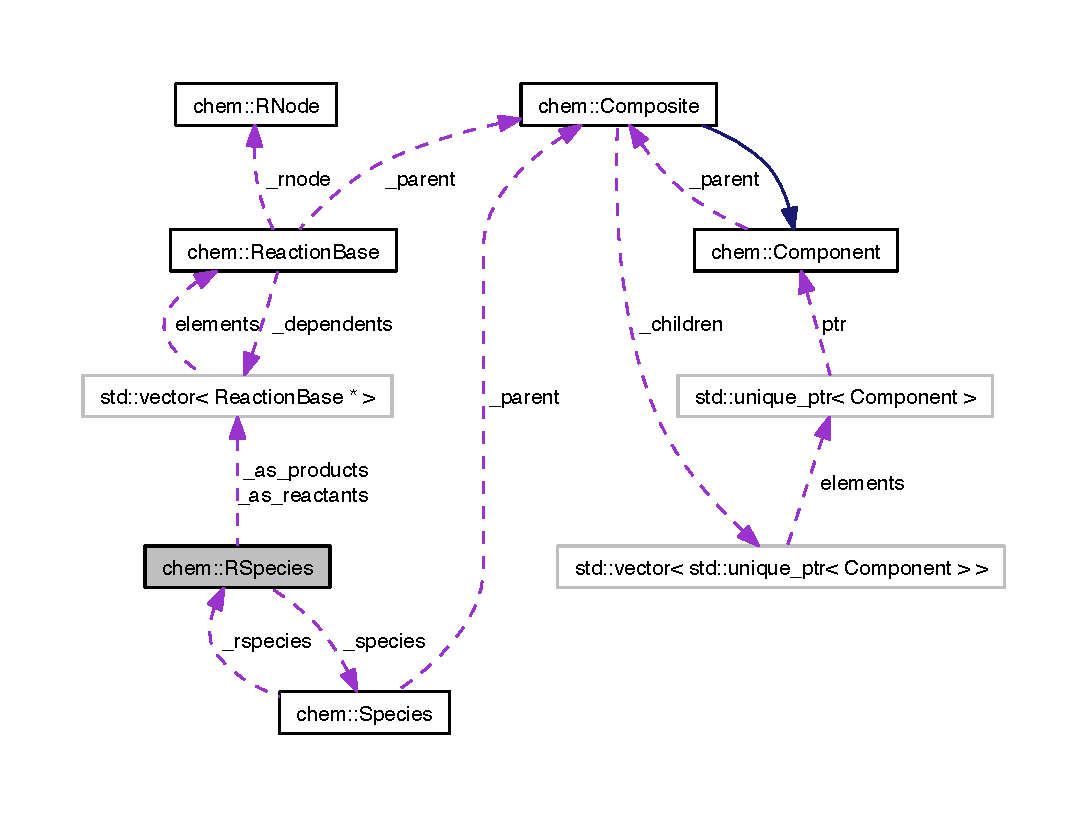
\includegraphics[width=350pt]{classchem_1_1RSpecies__coll__graph}
\end{center}
\end{figure}
\subsection*{Public Member Functions}
\begin{DoxyCompactItemize}
\item 
\hyperlink{classchem_1_1RSpecies_a66b426fdb13ec0e9ec61a96fadda465d}{R\-Species} (\hyperlink{classchem_1_1Species}{Species} \&parent, \hyperlink{common_8h_a3503f321fd36304ee274141275cca586}{species\-\_\-copy\-\_\-t} n=0, \hyperlink{common_8h_a3503f321fd36304ee274141275cca586}{species\-\_\-copy\-\_\-t} ulim=\hyperlink{common_8h_adaf831a0b61083f29adf8fc6e8edab35}{max\-\_\-ulim})
\begin{DoxyCompactList}\small\item\em Constructors. \end{DoxyCompactList}\item 
\hyperlink{classchem_1_1RSpecies_aed7fd68d286fab8190372a4dd98c14e3}{R\-Species} (const \hyperlink{classchem_1_1RSpecies}{R\-Species} \&r)
\begin{DoxyCompactList}\small\item\em deleted copy constructor -\/ each \hyperlink{classchem_1_1RSpecies}{R\-Species} is uniquely created by the parent \hyperlink{classchem_1_1Species}{Species} \end{DoxyCompactList}\item 
\hyperlink{classchem_1_1RSpecies_a06341eaeb5d6c30bf7812b08354b6b19}{R\-Species} (\hyperlink{classchem_1_1RSpecies}{R\-Species} \&\&r)
\begin{DoxyCompactList}\small\item\em deleted move constructor -\/ each \hyperlink{classchem_1_1RSpecies}{R\-Species} is uniquely created by the parent \hyperlink{classchem_1_1Species}{Species} \end{DoxyCompactList}\item 
\hyperlink{classchem_1_1RSpecies}{R\-Species} \& \hyperlink{classchem_1_1RSpecies_a2779fcf9c5103251aa87e7b466ba7752}{operator=} (\hyperlink{classchem_1_1RSpecies}{R\-Species} \&)
\begin{DoxyCompactList}\small\item\em deleted assignment operator -\/ each \hyperlink{classchem_1_1RSpecies}{R\-Species} is uniquely created by the parent \hyperlink{classchem_1_1Species}{Species} \end{DoxyCompactList}\item 
void \hyperlink{classchem_1_1RSpecies_a7939d5255e97d125821f657cadb48bc2}{set\-N} (\hyperlink{common_8h_a3503f321fd36304ee274141275cca586}{species\-\_\-copy\-\_\-t} n)
\begin{DoxyCompactList}\small\item\em Sets the copy number for this \hyperlink{classchem_1_1RSpecies}{R\-Species}. \end{DoxyCompactList}\item 
void \hyperlink{classchem_1_1RSpecies_a13c47ccb546b64f83ac09734c286fcd2}{set\-Upper\-Limit\-For\-N} (\hyperlink{common_8h_a3503f321fd36304ee274141275cca586}{species\-\_\-copy\-\_\-t} ulim)
\begin{DoxyCompactList}\small\item\em Sets the upper limit for the copy number of this \hyperlink{classchem_1_1RSpecies}{R\-Species}. \end{DoxyCompactList}\item 
\hyperlink{common_8h_a3503f321fd36304ee274141275cca586}{species\-\_\-copy\-\_\-t} \hyperlink{classchem_1_1RSpecies_ad233880e065382e598a95e75d401d9eb}{get\-Upper\-Limit\-For\-N} () const 
\begin{DoxyCompactList}\small\item\em Return the upper limit for the copy number of this \hyperlink{classchem_1_1RSpecies}{R\-Species}. \end{DoxyCompactList}\item 
void \hyperlink{classchem_1_1RSpecies_ae721e3c649a12e0a81bc6b77afe23f38}{up} ()
\begin{DoxyCompactList}\small\item\em Increases the copy number by 1. \end{DoxyCompactList}\item 
void \hyperlink{classchem_1_1RSpecies_a0b9db54a1407d689be7477e77b4bb1c6}{down} ()
\begin{DoxyCompactList}\small\item\em Decreases the copy number by 1. \end{DoxyCompactList}\item 
void \hyperlink{classchem_1_1RSpecies_a2f69141d801e4660ab411953fef74ea2}{add\-As\-Reactant} (\hyperlink{classchem_1_1ReactionBase}{Reaction\-Base} $\ast$r)
\item 
void \hyperlink{classchem_1_1RSpecies_a0df14f94c944f38f8794dc9229f8079c}{add\-As\-Product} (\hyperlink{classchem_1_1ReactionBase}{Reaction\-Base} $\ast$r)
\item 
void \hyperlink{classchem_1_1RSpecies_ab8f32e15791cfddea7cf4cac5a39c0fa}{remove\-As\-Reactant} (const \hyperlink{classchem_1_1ReactionBase}{Reaction\-Base} $\ast$r)
\item 
void \hyperlink{classchem_1_1RSpecies_a951496132075bd03ba51ba4d753f0d7f}{remove\-As\-Product} (const \hyperlink{classchem_1_1ReactionBase}{Reaction\-Base} $\ast$r)
\item 
void \hyperlink{classchem_1_1RSpecies_a1589cd0e045a084a32dff4a02612d4a3}{activate\-Assoc\-Reactant\-Reactions} ()
\item 
void \hyperlink{classchem_1_1RSpecies_ab275b0c9fb9352abe35a3bd68f3917fb}{activate\-Assoc\-Product\-Reactions} ()
\item 
void \hyperlink{classchem_1_1RSpecies_a0c33c29f86ee16b84151bc5f38953076}{passivate\-Assoc\-Reactant\-Reactions} ()
\item 
void \hyperlink{classchem_1_1RSpecies_aff8862396958db832848c94135282f1e}{passivate\-Assoc\-Product\-Reactions} ()
\item 
void \hyperlink{classchem_1_1RSpecies_a0beefdc1ec28646df87b0690a2d66734}{start\-Signaling} ()
\begin{DoxyCompactList}\small\item\em Set the signaling behavior of this \hyperlink{classchem_1_1RSpecies}{R\-Species}. \end{DoxyCompactList}\item 
void \hyperlink{classchem_1_1RSpecies_a3519759c28c5d50108753ebe6c67a537}{stop\-Signaling} ()
\begin{DoxyCompactList}\small\item\em Destroy the signal associated with this \hyperlink{classchem_1_1RSpecies}{R\-Species}; all associated slots will be destroyed. \end{DoxyCompactList}\item 
\hyperlink{classchem_1_1RSpecies_a3c875e360f7f53b2ca8bd30f7dbbb7ed}{$\sim$\-R\-Species} ()
\begin{DoxyCompactList}\small\item\em It is required that all \hyperlink{classchem_1_1Reaction}{Reactions} associated with this \hyperlink{classchem_1_1RSpecies}{R\-Species} are destructed before this \hyperlink{classchem_1_1RSpecies}{R\-Species} is destructed. \end{DoxyCompactList}\item 
void \hyperlink{classchem_1_1RSpecies_afaee31bbc312ca6fa84a9ffc02457611}{emit\-Signal} (int delta)
\begin{DoxyCompactList}\small\item\em Broadcasts signal indicating that the copy number of this \hyperlink{classchem_1_1RSpecies}{R\-Species} has changed This method should usually called by the code which runs the chemical dynamics (i.\-e. \end{DoxyCompactList}\item 
bool \hyperlink{classchem_1_1RSpecies_a652a2d0f305a8ab84305ff1dd1fd41b8}{is\-Signaling} () const 
\begin{DoxyCompactList}\small\item\em Return true if this \hyperlink{classchem_1_1RSpecies}{R\-Species} emits signals on copy number change. \end{DoxyCompactList}\item 
\hyperlink{common_8h_a3503f321fd36304ee274141275cca586}{species\-\_\-copy\-\_\-t} \hyperlink{classchem_1_1RSpecies_a5a96cf2a67af375c6471dfa5a21990f8}{get\-N} () const 
\begin{DoxyCompactList}\small\item\em Return the current copy number of this \hyperlink{classchem_1_1RSpecies}{R\-Species}. \end{DoxyCompactList}\item 
\hyperlink{classchem_1_1Species}{Species} \& \hyperlink{classchem_1_1RSpecies_a585ae6da09ba09c824aac7a0fcddd748}{get\-Species} ()
\begin{DoxyCompactList}\small\item\em return parent \hyperlink{classchem_1_1Species}{Species} as a reference \end{DoxyCompactList}\item 
const \hyperlink{classchem_1_1Species}{Species} \& \hyperlink{classchem_1_1RSpecies_a74953c2446c0261fc5732a63e3392a15}{get\-Species} () const 
\begin{DoxyCompactList}\small\item\em return parent \hyperlink{classchem_1_1Species}{Species} as a const reference \end{DoxyCompactList}\item 
std\-::string \hyperlink{classchem_1_1RSpecies_af4e42cfd817f05b2de169275e3496399}{get\-Full\-Name} () const 
\begin{DoxyCompactList}\small\item\em Return the full name of this \hyperlink{classchem_1_1Species}{Species} in a std\-::string format (e.\-g. \char`\"{}\-Arp2/3\{\-Bulk\}\char`\"{}. \end{DoxyCompactList}\item 
std\-::vector$<$ \hyperlink{classchem_1_1ReactionBase}{Reaction\-Base} $\ast$ $>$ \hyperlink{classchem_1_1RSpecies_a777147e17b1ef1e733cd35a1d2aa98ba}{Reactant\-Reactions} ()
\begin{DoxyCompactList}\small\item\em Return std\-::vector$<$\-Reaction\-Base $\ast$$>$, which contains pointers to all \hyperlink{classchem_1_1Reaction}{Reactions} where this \hyperlink{classchem_1_1RSpecies}{R\-Species} is involved as a Reactant. \end{DoxyCompactList}\item 
std\-::vector$<$ \hyperlink{classchem_1_1ReactionBase}{Reaction\-Base} $\ast$ $>$ \hyperlink{classchem_1_1RSpecies_ab978fcc67f44cf5a2aba3d8281f57dcf}{Product\-Reactions} ()
\begin{DoxyCompactList}\small\item\em Return std\-::vector$<$\-Reaction\-Base $\ast$$>$, which contains pointers to all \hyperlink{classchem_1_1Reaction}{Reactions} where this \hyperlink{classchem_1_1RSpecies}{R\-Species} is involved as a Product. \end{DoxyCompactList}\item 
\hyperlink{namespacechem_a0decff3bb0047ac3a45bc12163f063e4}{vr\-\_\-iterator} \hyperlink{classchem_1_1RSpecies_abb162e65b6a0bb4953be60299e23a8e1}{begin\-Reactant\-Reactions} ()
\begin{DoxyCompactList}\small\item\em Return std\-::vector$<$\-Reaction\-Base $\ast$$>$\-::iterator, which points to the beginning of all \hyperlink{classchem_1_1Reaction}{Reactions} where this \hyperlink{classchem_1_1RSpecies}{R\-Species} is involved as a Reactant. \end{DoxyCompactList}\item 
\hyperlink{namespacechem_a0decff3bb0047ac3a45bc12163f063e4}{vr\-\_\-iterator} \hyperlink{classchem_1_1RSpecies_a28a722faa4f1784cf42cb1aeadee9bcb}{begin\-Product\-Reactions} ()
\begin{DoxyCompactList}\small\item\em Return std\-::vector$<$\-Reaction\-Base $\ast$$>$\-::iterator, which points to the beginning of all \hyperlink{classchem_1_1Reaction}{Reactions} where this \hyperlink{classchem_1_1RSpecies}{R\-Species} is involved as a Product. \end{DoxyCompactList}\item 
\hyperlink{namespacechem_a0decff3bb0047ac3a45bc12163f063e4}{vr\-\_\-iterator} \hyperlink{classchem_1_1RSpecies_a1b228d34e6277a15f672247480f4b51a}{end\-Reactant\-Reactions} ()
\begin{DoxyCompactList}\small\item\em Return std\-::vector$<$\-Reaction\-Base $\ast$$>$\-::iterator, which points to the end of all \hyperlink{classchem_1_1Reaction}{Reactions} where this \hyperlink{classchem_1_1RSpecies}{R\-Species} is involved as a Reactant. \end{DoxyCompactList}\item 
\hyperlink{namespacechem_a0decff3bb0047ac3a45bc12163f063e4}{vr\-\_\-iterator} \hyperlink{classchem_1_1RSpecies_a1b3db9e6c2246f6d1b4d98d344ff9e9e}{end\-Product\-Reactions} ()
\begin{DoxyCompactList}\small\item\em Return std\-::vector$<$\-Reaction\-Base $\ast$$>$\-::iterator, which points to the end of all \hyperlink{classchem_1_1Reaction}{Reactions} where this \hyperlink{classchem_1_1RSpecies}{R\-Species} is involved as a Product. \end{DoxyCompactList}\end{DoxyCompactItemize}
\subsection*{Private Attributes}
\begin{DoxyCompactItemize}
\item 
friend \hyperlink{classchem_1_1RSpecies_af22c5fa6d6a8be2cd26b77fc4cbb820f}{Species}
\item 
std\-::vector$<$ \hyperlink{classchem_1_1ReactionBase}{Reaction\-Base} $\ast$ $>$ \hyperlink{classchem_1_1RSpecies_a7ffda464bbe610c372cac83e6e735023}{\-\_\-as\-\_\-reactants}
\begin{DoxyCompactList}\small\item\em Reactions calls \hyperlink{classchem_1_1RSpecies_a2f69141d801e4660ab411953fef74ea2}{add\-As\-Reactant()}, \hyperlink{classchem_1_1RSpecies_ab8f32e15791cfddea7cf4cac5a39c0fa}{remove\-As\-Reactant()} -\/ which other classes should not call. \end{DoxyCompactList}\item 
std\-::vector$<$ \hyperlink{classchem_1_1ReactionBase}{Reaction\-Base} $\ast$ $>$ \hyperlink{classchem_1_1RSpecies_ad4d3712865ed15fd9b581810ffe1b0e7}{\-\_\-as\-\_\-products}
\begin{DoxyCompactList}\small\item\em a vector of \hyperlink{classchem_1_1Reaction}{Reactions} where this \hyperlink{classchem_1_1RSpecies}{R\-Species} is a Product \end{DoxyCompactList}\item 
\hyperlink{classchem_1_1Species}{Species} \& \hyperlink{classchem_1_1RSpecies_a3a979b9226800417c7aad81a2162fac5}{\-\_\-species}
\begin{DoxyCompactList}\small\item\em reference to the {\bfseries parent} \hyperlink{classchem_1_1Species}{Species} object \end{DoxyCompactList}\item 
\hyperlink{common_8h_a3503f321fd36304ee274141275cca586}{species\-\_\-copy\-\_\-t} \hyperlink{classchem_1_1RSpecies_a60e53ebfe464923452c54322dfd479dc}{\-\_\-n}
\begin{DoxyCompactList}\small\item\em Current copy number of this \hyperlink{classchem_1_1RSpecies}{R\-Species}. \end{DoxyCompactList}\item 
\hyperlink{common_8h_a3503f321fd36304ee274141275cca586}{species\-\_\-copy\-\_\-t} \hyperlink{classchem_1_1RSpecies_a189084cfe75e004f42a6a27b2c1c09ad}{\-\_\-ulim}
\begin{DoxyCompactList}\small\item\em Upper limit for the copy number, afterwards all reactions leading to further accum. are turned off. \end{DoxyCompactList}\item 
\hyperlink{namespacechem_a6cb4144586460e7b7ae0dffdf08eb57c}{R\-Species\-Copy\-N\-Changed\-Signal} $\ast$ \hyperlink{classchem_1_1RSpecies_acd60296c77857284cd935cb6faaf4200}{\-\_\-signal}
\begin{DoxyCompactList}\small\item\em Can be used to broadcast a signal associated with change of n of. \end{DoxyCompactList}\end{DoxyCompactItemize}


\subsection{Detailed Description}
\hyperlink{classchem_1_1RSpecies}{R\-Species} class represents the reactive aspect of chemical molecules. It tracks their copy number and can be used in \hyperlink{classchem_1_1Reaction}{Reactions}. 

This class represents the reactivity of chemical species. The name \hyperlink{classchem_1_1RSpecies}{R\-Species} stems from reacting species. \hyperlink{classchem_1_1RSpecies}{R\-Species} tracks the copy number of molecules and the \hyperlink{classchem_1_1Reaction}{Reactions} in which it is involed (\begin{DoxySeeAlso}{See also}
\hyperlink{classchem_1_1Reaction}{Reaction}). 
\end{DoxySeeAlso}
\begin{DoxyNote}{Note}
Each intantiation of \hyperlink{classchem_1_1RSpecies}{R\-Species} is unique, and hence, cannot be neither copied nor moved (C++11). This has significant implications -\/ e.\-g., \hyperlink{classchem_1_1RSpecies}{R\-Species} cannot be used in std\-::vector$<$\-R\-Species$>$. Instead, one should use either std\-::vector$<$\-R\-Species$\ast$$>$ if not owning the \hyperlink{classchem_1_1RSpecies}{R\-Species} pointers, or std\-::vector$<$std\-::unique\-\_\-ptr$<$\-R\-Species$>$$>$ if owning the \hyperlink{classchem_1_1RSpecies}{R\-Species} pointers. A special allocator can be written such that dynamically allocated \hyperlink{classchem_1_1RSpecies}{R\-Species} (through new), are arranged contigiously in memory. 
\end{DoxyNote}


Definition at line 57 of file R\-Species.\-h.



\subsection{Constructor \& Destructor Documentation}
\hypertarget{classchem_1_1RSpecies_a66b426fdb13ec0e9ec61a96fadda465d}{\index{chem\-::\-R\-Species@{chem\-::\-R\-Species}!R\-Species@{R\-Species}}
\index{R\-Species@{R\-Species}!chem::RSpecies@{chem\-::\-R\-Species}}
\subsubsection[{R\-Species}]{\setlength{\rightskip}{0pt plus 5cm}{\bf chem\-::\-R\-Species\-::\-R\-Species} (
\begin{DoxyParamCaption}
\item[{{\bf Species} \&}]{parent, }
\item[{{\bf species\-\_\-copy\-\_\-t}}]{n = {\ttfamily 0}, }
\item[{{\bf species\-\_\-copy\-\_\-t}}]{ulim = {\ttfamily {\bf max\-\_\-ulim}}}
\end{DoxyParamCaption}
)\hspace{0.3cm}{\ttfamily  \mbox{[}inline\mbox{]}}}}\label{classchem_1_1RSpecies_a66b426fdb13ec0e9ec61a96fadda465d}


Constructors. 


\begin{DoxyParams}{Parameters}
{\em parent} & -\/ the \hyperlink{classchem_1_1Species}{Species} object to which this \hyperlink{classchem_1_1RSpecies}{R\-Species} belongs \\
\hline
{\em n} & -\/ copy number \\
\hline
\end{DoxyParams}


Definition at line 76 of file R\-Species.\-h.



References \-\_\-signal, and \-\_\-ulim.

\hypertarget{classchem_1_1RSpecies_aed7fd68d286fab8190372a4dd98c14e3}{\index{chem\-::\-R\-Species@{chem\-::\-R\-Species}!R\-Species@{R\-Species}}
\index{R\-Species@{R\-Species}!chem::RSpecies@{chem\-::\-R\-Species}}
\subsubsection[{R\-Species}]{\setlength{\rightskip}{0pt plus 5cm}{\bf chem\-::\-R\-Species\-::\-R\-Species} (
\begin{DoxyParamCaption}
\item[{const {\bf R\-Species} \&}]{r}
\end{DoxyParamCaption}
)}}\label{classchem_1_1RSpecies_aed7fd68d286fab8190372a4dd98c14e3}


deleted copy constructor -\/ each \hyperlink{classchem_1_1RSpecies}{R\-Species} is uniquely created by the parent \hyperlink{classchem_1_1Species}{Species} 

\hypertarget{classchem_1_1RSpecies_a06341eaeb5d6c30bf7812b08354b6b19}{\index{chem\-::\-R\-Species@{chem\-::\-R\-Species}!R\-Species@{R\-Species}}
\index{R\-Species@{R\-Species}!chem::RSpecies@{chem\-::\-R\-Species}}
\subsubsection[{R\-Species}]{\setlength{\rightskip}{0pt plus 5cm}{\bf chem\-::\-R\-Species\-::\-R\-Species} (
\begin{DoxyParamCaption}
\item[{{\bf R\-Species} \&\&}]{r}
\end{DoxyParamCaption}
)}}\label{classchem_1_1RSpecies_a06341eaeb5d6c30bf7812b08354b6b19}


deleted move constructor -\/ each \hyperlink{classchem_1_1RSpecies}{R\-Species} is uniquely created by the parent \hyperlink{classchem_1_1Species}{Species} 

\hypertarget{classchem_1_1RSpecies_a3c875e360f7f53b2ca8bd30f7dbbb7ed}{\index{chem\-::\-R\-Species@{chem\-::\-R\-Species}!$\sim$\-R\-Species@{$\sim$\-R\-Species}}
\index{$\sim$\-R\-Species@{$\sim$\-R\-Species}!chem::RSpecies@{chem\-::\-R\-Species}}
\subsubsection[{$\sim$\-R\-Species}]{\setlength{\rightskip}{0pt plus 5cm}{\bf chem\-::\-R\-Species\-::$\sim$\-R\-Species} (
\begin{DoxyParamCaption}
{}
\end{DoxyParamCaption}
)\hspace{0.3cm}{\ttfamily  \mbox{[}inline\mbox{]}}}}\label{classchem_1_1RSpecies_a3c875e360f7f53b2ca8bd30f7dbbb7ed}


It is required that all \hyperlink{classchem_1_1Reaction}{Reactions} associated with this \hyperlink{classchem_1_1RSpecies}{R\-Species} are destructed before this \hyperlink{classchem_1_1RSpecies}{R\-Species} is destructed. 

Most of the time, this will occur naturally. If not, an assertion will ungracefully terminate the program. 

Definition at line 202 of file R\-Species.\-h.



References \-\_\-as\-\_\-products, \-\_\-as\-\_\-reactants, and \-\_\-signal.



\subsection{Member Function Documentation}
\hypertarget{classchem_1_1RSpecies_ab275b0c9fb9352abe35a3bd68f3917fb}{\index{chem\-::\-R\-Species@{chem\-::\-R\-Species}!activate\-Assoc\-Product\-Reactions@{activate\-Assoc\-Product\-Reactions}}
\index{activate\-Assoc\-Product\-Reactions@{activate\-Assoc\-Product\-Reactions}!chem::RSpecies@{chem\-::\-R\-Species}}
\subsubsection[{activate\-Assoc\-Product\-Reactions}]{\setlength{\rightskip}{0pt plus 5cm}void {\bf chem\-::\-R\-Species\-::activate\-Assoc\-Product\-Reactions} (
\begin{DoxyParamCaption}
{}
\end{DoxyParamCaption}
)}}\label{classchem_1_1RSpecies_ab275b0c9fb9352abe35a3bd68f3917fb}
Attempts to activate previously passivated \hyperlink{classchem_1_1Reaction}{Reactions} where this \hyperlink{classchem_1_1RSpecies}{R\-Species} is involved as a Product. Usually, the \hyperlink{classchem_1_1Reaction}{Reaction} was first passivated, for example if the \hyperlink{classchem_1_1RSpecies}{R\-Species} copy number of one of the reactants went up to max\-\_\-ulim. 

Definition at line 61 of file R\-Species.\-cpp.



Referenced by down().

\hypertarget{classchem_1_1RSpecies_a1589cd0e045a084a32dff4a02612d4a3}{\index{chem\-::\-R\-Species@{chem\-::\-R\-Species}!activate\-Assoc\-Reactant\-Reactions@{activate\-Assoc\-Reactant\-Reactions}}
\index{activate\-Assoc\-Reactant\-Reactions@{activate\-Assoc\-Reactant\-Reactions}!chem::RSpecies@{chem\-::\-R\-Species}}
\subsubsection[{activate\-Assoc\-Reactant\-Reactions}]{\setlength{\rightskip}{0pt plus 5cm}void {\bf chem\-::\-R\-Species\-::activate\-Assoc\-Reactant\-Reactions} (
\begin{DoxyParamCaption}
{}
\end{DoxyParamCaption}
)}}\label{classchem_1_1RSpecies_a1589cd0e045a084a32dff4a02612d4a3}
Attempts to activate previously passivated \hyperlink{classchem_1_1Reaction}{Reactions} where this \hyperlink{classchem_1_1RSpecies}{R\-Species} is involved as a Reactant. Usually, the \hyperlink{classchem_1_1Reaction}{Reaction} was first passivated, for example if the \hyperlink{classchem_1_1RSpecies}{R\-Species} copy number of one of the reactants dropeed to zero. This attempt may not succeed if there are still other reactants in the same \hyperlink{classchem_1_1Reaction}{Reaction} with zero copy count. 

Definition at line 56 of file R\-Species.\-cpp.



Referenced by up().

\hypertarget{classchem_1_1RSpecies_a0df14f94c944f38f8794dc9229f8079c}{\index{chem\-::\-R\-Species@{chem\-::\-R\-Species}!add\-As\-Product@{add\-As\-Product}}
\index{add\-As\-Product@{add\-As\-Product}!chem::RSpecies@{chem\-::\-R\-Species}}
\subsubsection[{add\-As\-Product}]{\setlength{\rightskip}{0pt plus 5cm}void {\bf chem\-::\-R\-Species\-::add\-As\-Product} (
\begin{DoxyParamCaption}
\item[{{\bf Reaction\-Base} $\ast$}]{r}
\end{DoxyParamCaption}
)\hspace{0.3cm}{\ttfamily  \mbox{[}inline\mbox{]}}}}\label{classchem_1_1RSpecies_a0df14f94c944f38f8794dc9229f8079c}


Definition at line 153 of file R\-Species.\-h.



References \-\_\-as\-\_\-products.

\hypertarget{classchem_1_1RSpecies_a2f69141d801e4660ab411953fef74ea2}{\index{chem\-::\-R\-Species@{chem\-::\-R\-Species}!add\-As\-Reactant@{add\-As\-Reactant}}
\index{add\-As\-Reactant@{add\-As\-Reactant}!chem::RSpecies@{chem\-::\-R\-Species}}
\subsubsection[{add\-As\-Reactant}]{\setlength{\rightskip}{0pt plus 5cm}void {\bf chem\-::\-R\-Species\-::add\-As\-Reactant} (
\begin{DoxyParamCaption}
\item[{{\bf Reaction\-Base} $\ast$}]{r}
\end{DoxyParamCaption}
)\hspace{0.3cm}{\ttfamily  \mbox{[}inline\mbox{]}}}}\label{classchem_1_1RSpecies_a2f69141d801e4660ab411953fef74ea2}


Definition at line 149 of file R\-Species.\-h.



References \-\_\-as\-\_\-reactants.

\hypertarget{classchem_1_1RSpecies_a28a722faa4f1784cf42cb1aeadee9bcb}{\index{chem\-::\-R\-Species@{chem\-::\-R\-Species}!begin\-Product\-Reactions@{begin\-Product\-Reactions}}
\index{begin\-Product\-Reactions@{begin\-Product\-Reactions}!chem::RSpecies@{chem\-::\-R\-Species}}
\subsubsection[{begin\-Product\-Reactions}]{\setlength{\rightskip}{0pt plus 5cm}{\bf vr\-\_\-iterator} {\bf chem\-::\-R\-Species\-::begin\-Product\-Reactions} (
\begin{DoxyParamCaption}
{}
\end{DoxyParamCaption}
)\hspace{0.3cm}{\ttfamily  \mbox{[}inline\mbox{]}}}}\label{classchem_1_1RSpecies_a28a722faa4f1784cf42cb1aeadee9bcb}


Return std\-::vector$<$\-Reaction\-Base $\ast$$>$\-::iterator, which points to the beginning of all \hyperlink{classchem_1_1Reaction}{Reactions} where this \hyperlink{classchem_1_1RSpecies}{R\-Species} is involved as a Product. 



Definition at line 249 of file R\-Species.\-h.



References \-\_\-as\-\_\-products.



Referenced by chem\-::\-Reaction$<$ M, N $>$\-::activate\-Reaction\-Unconditional\-Impl(), and chem\-::\-Reaction$<$ M, N $>$\-::passivate\-Reaction\-Impl().

\hypertarget{classchem_1_1RSpecies_abb162e65b6a0bb4953be60299e23a8e1}{\index{chem\-::\-R\-Species@{chem\-::\-R\-Species}!begin\-Reactant\-Reactions@{begin\-Reactant\-Reactions}}
\index{begin\-Reactant\-Reactions@{begin\-Reactant\-Reactions}!chem::RSpecies@{chem\-::\-R\-Species}}
\subsubsection[{begin\-Reactant\-Reactions}]{\setlength{\rightskip}{0pt plus 5cm}{\bf vr\-\_\-iterator} {\bf chem\-::\-R\-Species\-::begin\-Reactant\-Reactions} (
\begin{DoxyParamCaption}
{}
\end{DoxyParamCaption}
)\hspace{0.3cm}{\ttfamily  \mbox{[}inline\mbox{]}}}}\label{classchem_1_1RSpecies_abb162e65b6a0bb4953be60299e23a8e1}


Return std\-::vector$<$\-Reaction\-Base $\ast$$>$\-::iterator, which points to the beginning of all \hyperlink{classchem_1_1Reaction}{Reactions} where this \hyperlink{classchem_1_1RSpecies}{R\-Species} is involved as a Reactant. 



Definition at line 245 of file R\-Species.\-h.



References \-\_\-as\-\_\-reactants.



Referenced by chem\-::\-Reaction$<$ M, N $>$\-::activate\-Reaction\-Unconditional\-Impl(), and chem\-::\-Reaction$<$ M, N $>$\-::passivate\-Reaction\-Impl().

\hypertarget{classchem_1_1RSpecies_a0b9db54a1407d689be7477e77b4bb1c6}{\index{chem\-::\-R\-Species@{chem\-::\-R\-Species}!down@{down}}
\index{down@{down}!chem::RSpecies@{chem\-::\-R\-Species}}
\subsubsection[{down}]{\setlength{\rightskip}{0pt plus 5cm}void {\bf chem\-::\-R\-Species\-::down} (
\begin{DoxyParamCaption}
{}
\end{DoxyParamCaption}
)\hspace{0.3cm}{\ttfamily  \mbox{[}inline\mbox{]}}}}\label{classchem_1_1RSpecies_a0b9db54a1407d689be7477e77b4bb1c6}


Decreases the copy number by 1. 

If the copy number changes becomes 0, calls a \char`\"{}callback\char`\"{}-\/like method to passivate \hyperlink{classchem_1_1Reaction}{Reactions}, where this \hyperlink{classchem_1_1RSpecies}{R\-Species} is a Reactant. 

Definition at line 128 of file R\-Species.\-h.



References \-\_\-n, \-\_\-ulim, activate\-Assoc\-Product\-Reactions(), and passivate\-Assoc\-Reactant\-Reactions().

\hypertarget{classchem_1_1RSpecies_afaee31bbc312ca6fa84a9ffc02457611}{\index{chem\-::\-R\-Species@{chem\-::\-R\-Species}!emit\-Signal@{emit\-Signal}}
\index{emit\-Signal@{emit\-Signal}!chem::RSpecies@{chem\-::\-R\-Species}}
\subsubsection[{emit\-Signal}]{\setlength{\rightskip}{0pt plus 5cm}void {\bf chem\-::\-R\-Species\-::emit\-Signal} (
\begin{DoxyParamCaption}
\item[{int}]{delta}
\end{DoxyParamCaption}
)\hspace{0.3cm}{\ttfamily  \mbox{[}inline\mbox{]}}}}\label{classchem_1_1RSpecies_afaee31bbc312ca6fa84a9ffc02457611}


Broadcasts signal indicating that the copy number of this \hyperlink{classchem_1_1RSpecies}{R\-Species} has changed This method should usually called by the code which runs the chemical dynamics (i.\-e. 

Gillespie-\/like algorithm) 

Definition at line 214 of file R\-Species.\-h.



References is\-Signaling().

\hypertarget{classchem_1_1RSpecies_a1b3db9e6c2246f6d1b4d98d344ff9e9e}{\index{chem\-::\-R\-Species@{chem\-::\-R\-Species}!end\-Product\-Reactions@{end\-Product\-Reactions}}
\index{end\-Product\-Reactions@{end\-Product\-Reactions}!chem::RSpecies@{chem\-::\-R\-Species}}
\subsubsection[{end\-Product\-Reactions}]{\setlength{\rightskip}{0pt plus 5cm}{\bf vr\-\_\-iterator} {\bf chem\-::\-R\-Species\-::end\-Product\-Reactions} (
\begin{DoxyParamCaption}
{}
\end{DoxyParamCaption}
)\hspace{0.3cm}{\ttfamily  \mbox{[}inline\mbox{]}}}}\label{classchem_1_1RSpecies_a1b3db9e6c2246f6d1b4d98d344ff9e9e}


Return std\-::vector$<$\-Reaction\-Base $\ast$$>$\-::iterator, which points to the end of all \hyperlink{classchem_1_1Reaction}{Reactions} where this \hyperlink{classchem_1_1RSpecies}{R\-Species} is involved as a Product. 



Definition at line 257 of file R\-Species.\-h.



References \-\_\-as\-\_\-products.



Referenced by chem\-::\-Reaction$<$ M, N $>$\-::activate\-Reaction\-Unconditional\-Impl(), and chem\-::\-Reaction$<$ M, N $>$\-::passivate\-Reaction\-Impl().

\hypertarget{classchem_1_1RSpecies_a1b228d34e6277a15f672247480f4b51a}{\index{chem\-::\-R\-Species@{chem\-::\-R\-Species}!end\-Reactant\-Reactions@{end\-Reactant\-Reactions}}
\index{end\-Reactant\-Reactions@{end\-Reactant\-Reactions}!chem::RSpecies@{chem\-::\-R\-Species}}
\subsubsection[{end\-Reactant\-Reactions}]{\setlength{\rightskip}{0pt plus 5cm}{\bf vr\-\_\-iterator} {\bf chem\-::\-R\-Species\-::end\-Reactant\-Reactions} (
\begin{DoxyParamCaption}
{}
\end{DoxyParamCaption}
)\hspace{0.3cm}{\ttfamily  \mbox{[}inline\mbox{]}}}}\label{classchem_1_1RSpecies_a1b228d34e6277a15f672247480f4b51a}


Return std\-::vector$<$\-Reaction\-Base $\ast$$>$\-::iterator, which points to the end of all \hyperlink{classchem_1_1Reaction}{Reactions} where this \hyperlink{classchem_1_1RSpecies}{R\-Species} is involved as a Reactant. 



Definition at line 253 of file R\-Species.\-h.



References \-\_\-as\-\_\-reactants.



Referenced by chem\-::\-Reaction$<$ M, N $>$\-::activate\-Reaction\-Unconditional\-Impl(), and chem\-::\-Reaction$<$ M, N $>$\-::passivate\-Reaction\-Impl().

\hypertarget{classchem_1_1RSpecies_af4e42cfd817f05b2de169275e3496399}{\index{chem\-::\-R\-Species@{chem\-::\-R\-Species}!get\-Full\-Name@{get\-Full\-Name}}
\index{get\-Full\-Name@{get\-Full\-Name}!chem::RSpecies@{chem\-::\-R\-Species}}
\subsubsection[{get\-Full\-Name}]{\setlength{\rightskip}{0pt plus 5cm}std\-::string {\bf chem\-::\-R\-Species\-::get\-Full\-Name} (
\begin{DoxyParamCaption}
{}
\end{DoxyParamCaption}
) const}}\label{classchem_1_1RSpecies_af4e42cfd817f05b2de169275e3496399}


Return the full name of this \hyperlink{classchem_1_1Species}{Species} in a std\-::string format (e.\-g. \char`\"{}\-Arp2/3\{\-Bulk\}\char`\"{}. 



Definition at line 51 of file R\-Species.\-cpp.



Referenced by operator$<$$<$().

\hypertarget{classchem_1_1RSpecies_a5a96cf2a67af375c6471dfa5a21990f8}{\index{chem\-::\-R\-Species@{chem\-::\-R\-Species}!get\-N@{get\-N}}
\index{get\-N@{get\-N}!chem::RSpecies@{chem\-::\-R\-Species}}
\subsubsection[{get\-N}]{\setlength{\rightskip}{0pt plus 5cm}{\bf species\-\_\-copy\-\_\-t} {\bf chem\-::\-R\-Species\-::get\-N} (
\begin{DoxyParamCaption}
{}
\end{DoxyParamCaption}
) const\hspace{0.3cm}{\ttfamily  \mbox{[}inline\mbox{]}}}}\label{classchem_1_1RSpecies_a5a96cf2a67af375c6471dfa5a21990f8}


Return the current copy number of this \hyperlink{classchem_1_1RSpecies}{R\-Species}. 



Definition at line 224 of file R\-Species.\-h.



References \-\_\-n.



Referenced by chem\-::\-Species\-::get\-N(), and operator$<$$<$().

\hypertarget{classchem_1_1RSpecies_a585ae6da09ba09c824aac7a0fcddd748}{\index{chem\-::\-R\-Species@{chem\-::\-R\-Species}!get\-Species@{get\-Species}}
\index{get\-Species@{get\-Species}!chem::RSpecies@{chem\-::\-R\-Species}}
\subsubsection[{get\-Species}]{\setlength{\rightskip}{0pt plus 5cm}{\bf Species}\& {\bf chem\-::\-R\-Species\-::get\-Species} (
\begin{DoxyParamCaption}
{}
\end{DoxyParamCaption}
)\hspace{0.3cm}{\ttfamily  \mbox{[}inline\mbox{]}}}}\label{classchem_1_1RSpecies_a585ae6da09ba09c824aac7a0fcddd748}


return parent \hyperlink{classchem_1_1Species}{Species} as a reference 



Definition at line 227 of file R\-Species.\-h.



References \-\_\-species.



Referenced by chem\-::\-Reaction$<$ M, N $>$\-::is\-\_\-equal().

\hypertarget{classchem_1_1RSpecies_a74953c2446c0261fc5732a63e3392a15}{\index{chem\-::\-R\-Species@{chem\-::\-R\-Species}!get\-Species@{get\-Species}}
\index{get\-Species@{get\-Species}!chem::RSpecies@{chem\-::\-R\-Species}}
\subsubsection[{get\-Species}]{\setlength{\rightskip}{0pt plus 5cm}const {\bf Species}\& {\bf chem\-::\-R\-Species\-::get\-Species} (
\begin{DoxyParamCaption}
{}
\end{DoxyParamCaption}
) const\hspace{0.3cm}{\ttfamily  \mbox{[}inline\mbox{]}}}}\label{classchem_1_1RSpecies_a74953c2446c0261fc5732a63e3392a15}


return parent \hyperlink{classchem_1_1Species}{Species} as a const reference 



Definition at line 230 of file R\-Species.\-h.



References \-\_\-species.

\hypertarget{classchem_1_1RSpecies_ad233880e065382e598a95e75d401d9eb}{\index{chem\-::\-R\-Species@{chem\-::\-R\-Species}!get\-Upper\-Limit\-For\-N@{get\-Upper\-Limit\-For\-N}}
\index{get\-Upper\-Limit\-For\-N@{get\-Upper\-Limit\-For\-N}!chem::RSpecies@{chem\-::\-R\-Species}}
\subsubsection[{get\-Upper\-Limit\-For\-N}]{\setlength{\rightskip}{0pt plus 5cm}{\bf species\-\_\-copy\-\_\-t} {\bf chem\-::\-R\-Species\-::get\-Upper\-Limit\-For\-N} (
\begin{DoxyParamCaption}
{}
\end{DoxyParamCaption}
) const\hspace{0.3cm}{\ttfamily  \mbox{[}inline\mbox{]}}}}\label{classchem_1_1RSpecies_ad233880e065382e598a95e75d401d9eb}


Return the upper limit for the copy number of this \hyperlink{classchem_1_1RSpecies}{R\-Species}. 



Definition at line 107 of file R\-Species.\-h.



References \-\_\-ulim.



Referenced by chem\-::\-Species\-::get\-Upper\-Limit\-For\-N().

\hypertarget{classchem_1_1RSpecies_a652a2d0f305a8ab84305ff1dd1fd41b8}{\index{chem\-::\-R\-Species@{chem\-::\-R\-Species}!is\-Signaling@{is\-Signaling}}
\index{is\-Signaling@{is\-Signaling}!chem::RSpecies@{chem\-::\-R\-Species}}
\subsubsection[{is\-Signaling}]{\setlength{\rightskip}{0pt plus 5cm}bool {\bf chem\-::\-R\-Species\-::is\-Signaling} (
\begin{DoxyParamCaption}
{}
\end{DoxyParamCaption}
) const\hspace{0.3cm}{\ttfamily  \mbox{[}inline\mbox{]}}}}\label{classchem_1_1RSpecies_a652a2d0f305a8ab84305ff1dd1fd41b8}


Return true if this \hyperlink{classchem_1_1RSpecies}{R\-Species} emits signals on copy number change. 



Definition at line 220 of file R\-Species.\-h.



References \-\_\-signal.



Referenced by emit\-Signal(), and chem\-::\-Species\-::is\-Signaling().

\hypertarget{classchem_1_1RSpecies_a2779fcf9c5103251aa87e7b466ba7752}{\index{chem\-::\-R\-Species@{chem\-::\-R\-Species}!operator=@{operator=}}
\index{operator=@{operator=}!chem::RSpecies@{chem\-::\-R\-Species}}
\subsubsection[{operator=}]{\setlength{\rightskip}{0pt plus 5cm}{\bf R\-Species}\& chem\-::\-R\-Species\-::operator= (
\begin{DoxyParamCaption}
\item[{{\bf R\-Species} \&}]{}
\end{DoxyParamCaption}
)}}\label{classchem_1_1RSpecies_a2779fcf9c5103251aa87e7b466ba7752}


deleted assignment operator -\/ each \hyperlink{classchem_1_1RSpecies}{R\-Species} is uniquely created by the parent \hyperlink{classchem_1_1Species}{Species} 

\hypertarget{classchem_1_1RSpecies_aff8862396958db832848c94135282f1e}{\index{chem\-::\-R\-Species@{chem\-::\-R\-Species}!passivate\-Assoc\-Product\-Reactions@{passivate\-Assoc\-Product\-Reactions}}
\index{passivate\-Assoc\-Product\-Reactions@{passivate\-Assoc\-Product\-Reactions}!chem::RSpecies@{chem\-::\-R\-Species}}
\subsubsection[{passivate\-Assoc\-Product\-Reactions}]{\setlength{\rightskip}{0pt plus 5cm}void {\bf chem\-::\-R\-Species\-::passivate\-Assoc\-Product\-Reactions} (
\begin{DoxyParamCaption}
{}
\end{DoxyParamCaption}
)}}\label{classchem_1_1RSpecies_aff8862396958db832848c94135282f1e}
Passivates all \hyperlink{classchem_1_1Reaction}{Reactions} where this \hyperlink{classchem_1_1RSpecies}{R\-Species} is among the products. 

Definition at line 71 of file R\-Species.\-cpp.



Referenced by up().

\hypertarget{classchem_1_1RSpecies_a0c33c29f86ee16b84151bc5f38953076}{\index{chem\-::\-R\-Species@{chem\-::\-R\-Species}!passivate\-Assoc\-Reactant\-Reactions@{passivate\-Assoc\-Reactant\-Reactions}}
\index{passivate\-Assoc\-Reactant\-Reactions@{passivate\-Assoc\-Reactant\-Reactions}!chem::RSpecies@{chem\-::\-R\-Species}}
\subsubsection[{passivate\-Assoc\-Reactant\-Reactions}]{\setlength{\rightskip}{0pt plus 5cm}void {\bf chem\-::\-R\-Species\-::passivate\-Assoc\-Reactant\-Reactions} (
\begin{DoxyParamCaption}
{}
\end{DoxyParamCaption}
)}}\label{classchem_1_1RSpecies_a0c33c29f86ee16b84151bc5f38953076}
Passivates all \hyperlink{classchem_1_1Reaction}{Reactions} where this \hyperlink{classchem_1_1RSpecies}{R\-Species} is among the reactants. 

Definition at line 66 of file R\-Species.\-cpp.



Referenced by down().

\hypertarget{classchem_1_1RSpecies_ab978fcc67f44cf5a2aba3d8281f57dcf}{\index{chem\-::\-R\-Species@{chem\-::\-R\-Species}!Product\-Reactions@{Product\-Reactions}}
\index{Product\-Reactions@{Product\-Reactions}!chem::RSpecies@{chem\-::\-R\-Species}}
\subsubsection[{Product\-Reactions}]{\setlength{\rightskip}{0pt plus 5cm}std\-::vector$<${\bf Reaction\-Base} $\ast$$>$ {\bf chem\-::\-R\-Species\-::\-Product\-Reactions} (
\begin{DoxyParamCaption}
{}
\end{DoxyParamCaption}
)\hspace{0.3cm}{\ttfamily  \mbox{[}inline\mbox{]}}}}\label{classchem_1_1RSpecies_ab978fcc67f44cf5a2aba3d8281f57dcf}


Return std\-::vector$<$\-Reaction\-Base $\ast$$>$, which contains pointers to all \hyperlink{classchem_1_1Reaction}{Reactions} where this \hyperlink{classchem_1_1RSpecies}{R\-Species} is involved as a Product. 



Definition at line 241 of file R\-Species.\-h.



References \-\_\-as\-\_\-products.

\hypertarget{classchem_1_1RSpecies_a777147e17b1ef1e733cd35a1d2aa98ba}{\index{chem\-::\-R\-Species@{chem\-::\-R\-Species}!Reactant\-Reactions@{Reactant\-Reactions}}
\index{Reactant\-Reactions@{Reactant\-Reactions}!chem::RSpecies@{chem\-::\-R\-Species}}
\subsubsection[{Reactant\-Reactions}]{\setlength{\rightskip}{0pt plus 5cm}std\-::vector$<${\bf Reaction\-Base} $\ast$$>$ {\bf chem\-::\-R\-Species\-::\-Reactant\-Reactions} (
\begin{DoxyParamCaption}
{}
\end{DoxyParamCaption}
)\hspace{0.3cm}{\ttfamily  \mbox{[}inline\mbox{]}}}}\label{classchem_1_1RSpecies_a777147e17b1ef1e733cd35a1d2aa98ba}


Return std\-::vector$<$\-Reaction\-Base $\ast$$>$, which contains pointers to all \hyperlink{classchem_1_1Reaction}{Reactions} where this \hyperlink{classchem_1_1RSpecies}{R\-Species} is involved as a Reactant. 



Definition at line 237 of file R\-Species.\-h.



References \-\_\-as\-\_\-reactants.

\hypertarget{classchem_1_1RSpecies_a951496132075bd03ba51ba4d753f0d7f}{\index{chem\-::\-R\-Species@{chem\-::\-R\-Species}!remove\-As\-Product@{remove\-As\-Product}}
\index{remove\-As\-Product@{remove\-As\-Product}!chem::RSpecies@{chem\-::\-R\-Species}}
\subsubsection[{remove\-As\-Product}]{\setlength{\rightskip}{0pt plus 5cm}void {\bf chem\-::\-R\-Species\-::remove\-As\-Product} (
\begin{DoxyParamCaption}
\item[{const {\bf Reaction\-Base} $\ast$}]{r}
\end{DoxyParamCaption}
)\hspace{0.3cm}{\ttfamily  \mbox{[}inline\mbox{]}}}}\label{classchem_1_1RSpecies_a951496132075bd03ba51ba4d753f0d7f}


Definition at line 166 of file R\-Species.\-h.



References \-\_\-as\-\_\-products.

\hypertarget{classchem_1_1RSpecies_ab8f32e15791cfddea7cf4cac5a39c0fa}{\index{chem\-::\-R\-Species@{chem\-::\-R\-Species}!remove\-As\-Reactant@{remove\-As\-Reactant}}
\index{remove\-As\-Reactant@{remove\-As\-Reactant}!chem::RSpecies@{chem\-::\-R\-Species}}
\subsubsection[{remove\-As\-Reactant}]{\setlength{\rightskip}{0pt plus 5cm}void {\bf chem\-::\-R\-Species\-::remove\-As\-Reactant} (
\begin{DoxyParamCaption}
\item[{const {\bf Reaction\-Base} $\ast$}]{r}
\end{DoxyParamCaption}
)\hspace{0.3cm}{\ttfamily  \mbox{[}inline\mbox{]}}}}\label{classchem_1_1RSpecies_ab8f32e15791cfddea7cf4cac5a39c0fa}


Definition at line 157 of file R\-Species.\-h.



References \-\_\-as\-\_\-products, and \-\_\-as\-\_\-reactants.

\hypertarget{classchem_1_1RSpecies_a7939d5255e97d125821f657cadb48bc2}{\index{chem\-::\-R\-Species@{chem\-::\-R\-Species}!set\-N@{set\-N}}
\index{set\-N@{set\-N}!chem::RSpecies@{chem\-::\-R\-Species}}
\subsubsection[{set\-N}]{\setlength{\rightskip}{0pt plus 5cm}void {\bf chem\-::\-R\-Species\-::set\-N} (
\begin{DoxyParamCaption}
\item[{{\bf species\-\_\-copy\-\_\-t}}]{n}
\end{DoxyParamCaption}
)\hspace{0.3cm}{\ttfamily  \mbox{[}inline\mbox{]}}}}\label{classchem_1_1RSpecies_a7939d5255e97d125821f657cadb48bc2}


Sets the copy number for this \hyperlink{classchem_1_1RSpecies}{R\-Species}. 


\begin{DoxyParams}{Parameters}
{\em n} & should be a non-\/negative number, but no checking is done in run time \\
\hline
\end{DoxyParams}
\begin{DoxyNote}{Note}
The operation does not emit any signals about the copy number change. 
\end{DoxyNote}


Definition at line 99 of file R\-Species.\-h.



References \-\_\-n.



Referenced by chem\-::\-Species\-::set\-N().

\hypertarget{classchem_1_1RSpecies_a13c47ccb546b64f83ac09734c286fcd2}{\index{chem\-::\-R\-Species@{chem\-::\-R\-Species}!set\-Upper\-Limit\-For\-N@{set\-Upper\-Limit\-For\-N}}
\index{set\-Upper\-Limit\-For\-N@{set\-Upper\-Limit\-For\-N}!chem::RSpecies@{chem\-::\-R\-Species}}
\subsubsection[{set\-Upper\-Limit\-For\-N}]{\setlength{\rightskip}{0pt plus 5cm}void {\bf chem\-::\-R\-Species\-::set\-Upper\-Limit\-For\-N} (
\begin{DoxyParamCaption}
\item[{{\bf species\-\_\-copy\-\_\-t}}]{ulim}
\end{DoxyParamCaption}
)\hspace{0.3cm}{\ttfamily  \mbox{[}inline\mbox{]}}}}\label{classchem_1_1RSpecies_a13c47ccb546b64f83ac09734c286fcd2}


Sets the upper limit for the copy number of this \hyperlink{classchem_1_1RSpecies}{R\-Species}. 


\begin{DoxyParams}{Parameters}
{\em ulim} & should be a non-\/negative number, but no checking is done in run time \\
\hline
\end{DoxyParams}


Definition at line 104 of file R\-Species.\-h.



References \-\_\-ulim.

\hypertarget{classchem_1_1RSpecies_a0beefdc1ec28646df87b0690a2d66734}{\index{chem\-::\-R\-Species@{chem\-::\-R\-Species}!start\-Signaling@{start\-Signaling}}
\index{start\-Signaling@{start\-Signaling}!chem::RSpecies@{chem\-::\-R\-Species}}
\subsubsection[{start\-Signaling}]{\setlength{\rightskip}{0pt plus 5cm}void {\bf chem\-::\-R\-Species\-::start\-Signaling} (
\begin{DoxyParamCaption}
{}
\end{DoxyParamCaption}
)}}\label{classchem_1_1RSpecies_a0beefdc1ec28646df87b0690a2d66734}


Set the signaling behavior of this \hyperlink{classchem_1_1RSpecies}{R\-Species}. 



Definition at line 79 of file R\-Species.\-cpp.



Referenced by chem\-::\-Species\-::start\-Signaling().

\hypertarget{classchem_1_1RSpecies_a3519759c28c5d50108753ebe6c67a537}{\index{chem\-::\-R\-Species@{chem\-::\-R\-Species}!stop\-Signaling@{stop\-Signaling}}
\index{stop\-Signaling@{stop\-Signaling}!chem::RSpecies@{chem\-::\-R\-Species}}
\subsubsection[{stop\-Signaling}]{\setlength{\rightskip}{0pt plus 5cm}void {\bf chem\-::\-R\-Species\-::stop\-Signaling} (
\begin{DoxyParamCaption}
{}
\end{DoxyParamCaption}
)}}\label{classchem_1_1RSpecies_a3519759c28c5d50108753ebe6c67a537}


Destroy the signal associated with this \hyperlink{classchem_1_1RSpecies}{R\-Species}; all associated slots will be destroyed. 

\begin{DoxyNote}{Note}
To start signaling again, \hyperlink{classchem_1_1RSpecies_a0beefdc1ec28646df87b0690a2d66734}{start\-Signaling()} needs to be called 
\end{DoxyNote}


Definition at line 83 of file R\-Species.\-cpp.



Referenced by chem\-::\-Species\-::stop\-Signaling().

\hypertarget{classchem_1_1RSpecies_ae721e3c649a12e0a81bc6b77afe23f38}{\index{chem\-::\-R\-Species@{chem\-::\-R\-Species}!up@{up}}
\index{up@{up}!chem::RSpecies@{chem\-::\-R\-Species}}
\subsubsection[{up}]{\setlength{\rightskip}{0pt plus 5cm}void {\bf chem\-::\-R\-Species\-::up} (
\begin{DoxyParamCaption}
{}
\end{DoxyParamCaption}
)\hspace{0.3cm}{\ttfamily  \mbox{[}inline\mbox{]}}}}\label{classchem_1_1RSpecies_ae721e3c649a12e0a81bc6b77afe23f38}


Increases the copy number by 1. 

If the copy number changes from 0 to 1, calls a \char`\"{}callback\char`\"{}-\/like method to activated previously passivated \hyperlink{classchem_1_1Reaction}{Reactions}, where this \hyperlink{classchem_1_1RSpecies}{R\-Species} is a Reactant. 

Definition at line 112 of file R\-Species.\-h.



References \-\_\-n, \-\_\-ulim, activate\-Assoc\-Reactant\-Reactions(), and passivate\-Assoc\-Product\-Reactions().



\subsection{Member Data Documentation}
\hypertarget{classchem_1_1RSpecies_ad4d3712865ed15fd9b581810ffe1b0e7}{\index{chem\-::\-R\-Species@{chem\-::\-R\-Species}!\-\_\-as\-\_\-products@{\-\_\-as\-\_\-products}}
\index{\-\_\-as\-\_\-products@{\-\_\-as\-\_\-products}!chem::RSpecies@{chem\-::\-R\-Species}}
\subsubsection[{\-\_\-as\-\_\-products}]{\setlength{\rightskip}{0pt plus 5cm}std\-::vector$<${\bf Reaction\-Base} $\ast$$>$ {\bf chem\-::\-R\-Species\-::\-\_\-as\-\_\-products}\hspace{0.3cm}{\ttfamily  \mbox{[}private\mbox{]}}}}\label{classchem_1_1RSpecies_ad4d3712865ed15fd9b581810ffe1b0e7}


a vector of \hyperlink{classchem_1_1Reaction}{Reactions} where this \hyperlink{classchem_1_1RSpecies}{R\-Species} is a Product 



Definition at line 62 of file R\-Species.\-h.



Referenced by add\-As\-Product(), begin\-Product\-Reactions(), end\-Product\-Reactions(), Product\-Reactions(), remove\-As\-Product(), remove\-As\-Reactant(), and $\sim$\-R\-Species().

\hypertarget{classchem_1_1RSpecies_a7ffda464bbe610c372cac83e6e735023}{\index{chem\-::\-R\-Species@{chem\-::\-R\-Species}!\-\_\-as\-\_\-reactants@{\-\_\-as\-\_\-reactants}}
\index{\-\_\-as\-\_\-reactants@{\-\_\-as\-\_\-reactants}!chem::RSpecies@{chem\-::\-R\-Species}}
\subsubsection[{\-\_\-as\-\_\-reactants}]{\setlength{\rightskip}{0pt plus 5cm}std\-::vector$<${\bf Reaction\-Base} $\ast$$>$ {\bf chem\-::\-R\-Species\-::\-\_\-as\-\_\-reactants}\hspace{0.3cm}{\ttfamily  \mbox{[}private\mbox{]}}}}\label{classchem_1_1RSpecies_a7ffda464bbe610c372cac83e6e735023}


Reactions calls \hyperlink{classchem_1_1RSpecies_a2f69141d801e4660ab411953fef74ea2}{add\-As\-Reactant()}, \hyperlink{classchem_1_1RSpecies_ab8f32e15791cfddea7cf4cac5a39c0fa}{remove\-As\-Reactant()} -\/ which other classes should not call. 

a vector of \hyperlink{classchem_1_1Reaction}{Reactions} where this \hyperlink{classchem_1_1RSpecies}{R\-Species} is a Reactant 

Definition at line 61 of file R\-Species.\-h.



Referenced by add\-As\-Reactant(), begin\-Reactant\-Reactions(), end\-Reactant\-Reactions(), Reactant\-Reactions(), remove\-As\-Reactant(), and $\sim$\-R\-Species().

\hypertarget{classchem_1_1RSpecies_a60e53ebfe464923452c54322dfd479dc}{\index{chem\-::\-R\-Species@{chem\-::\-R\-Species}!\-\_\-n@{\-\_\-n}}
\index{\-\_\-n@{\-\_\-n}!chem::RSpecies@{chem\-::\-R\-Species}}
\subsubsection[{\-\_\-n}]{\setlength{\rightskip}{0pt plus 5cm}{\bf species\-\_\-copy\-\_\-t} {\bf chem\-::\-R\-Species\-::\-\_\-n}\hspace{0.3cm}{\ttfamily  \mbox{[}private\mbox{]}}}}\label{classchem_1_1RSpecies_a60e53ebfe464923452c54322dfd479dc}


Current copy number of this \hyperlink{classchem_1_1RSpecies}{R\-Species}. 



Definition at line 64 of file R\-Species.\-h.



Referenced by down(), get\-N(), set\-N(), and up().

\hypertarget{classchem_1_1RSpecies_acd60296c77857284cd935cb6faaf4200}{\index{chem\-::\-R\-Species@{chem\-::\-R\-Species}!\-\_\-signal@{\-\_\-signal}}
\index{\-\_\-signal@{\-\_\-signal}!chem::RSpecies@{chem\-::\-R\-Species}}
\subsubsection[{\-\_\-signal}]{\setlength{\rightskip}{0pt plus 5cm}{\bf R\-Species\-Copy\-N\-Changed\-Signal}$\ast$ {\bf chem\-::\-R\-Species\-::\-\_\-signal}\hspace{0.3cm}{\ttfamily  \mbox{[}private\mbox{]}}}}\label{classchem_1_1RSpecies_acd60296c77857284cd935cb6faaf4200}


Can be used to broadcast a signal associated with change of n of. 

this \hyperlink{classchem_1_1RSpecies}{R\-Species} (usually when a single step of this \hyperlink{classchem_1_1Reaction}{Reaction} occurs) 

Definition at line 69 of file R\-Species.\-h.



Referenced by chem\-::\-Species\-::connect(), is\-Signaling(), R\-Species(), and $\sim$\-R\-Species().

\hypertarget{classchem_1_1RSpecies_a3a979b9226800417c7aad81a2162fac5}{\index{chem\-::\-R\-Species@{chem\-::\-R\-Species}!\-\_\-species@{\-\_\-species}}
\index{\-\_\-species@{\-\_\-species}!chem::RSpecies@{chem\-::\-R\-Species}}
\subsubsection[{\-\_\-species}]{\setlength{\rightskip}{0pt plus 5cm}{\bf Species}\& {\bf chem\-::\-R\-Species\-::\-\_\-species}\hspace{0.3cm}{\ttfamily  \mbox{[}private\mbox{]}}}}\label{classchem_1_1RSpecies_a3a979b9226800417c7aad81a2162fac5}


reference to the {\bfseries parent} \hyperlink{classchem_1_1Species}{Species} object 



Definition at line 63 of file R\-Species.\-h.



Referenced by get\-Species().

\hypertarget{classchem_1_1RSpecies_a189084cfe75e004f42a6a27b2c1c09ad}{\index{chem\-::\-R\-Species@{chem\-::\-R\-Species}!\-\_\-ulim@{\-\_\-ulim}}
\index{\-\_\-ulim@{\-\_\-ulim}!chem::RSpecies@{chem\-::\-R\-Species}}
\subsubsection[{\-\_\-ulim}]{\setlength{\rightskip}{0pt plus 5cm}{\bf species\-\_\-copy\-\_\-t} {\bf chem\-::\-R\-Species\-::\-\_\-ulim}\hspace{0.3cm}{\ttfamily  \mbox{[}private\mbox{]}}}}\label{classchem_1_1RSpecies_a189084cfe75e004f42a6a27b2c1c09ad}


Upper limit for the copy number, afterwards all reactions leading to further accum. are turned off. 



Definition at line 66 of file R\-Species.\-h.



Referenced by down(), get\-Upper\-Limit\-For\-N(), R\-Species(), set\-Upper\-Limit\-For\-N(), and up().

\hypertarget{classchem_1_1RSpecies_af22c5fa6d6a8be2cd26b77fc4cbb820f}{\index{chem\-::\-R\-Species@{chem\-::\-R\-Species}!Species@{Species}}
\index{Species@{Species}!chem::RSpecies@{chem\-::\-R\-Species}}
\subsubsection[{Species}]{\setlength{\rightskip}{0pt plus 5cm}friend {\bf chem\-::\-R\-Species\-::\-Species}\hspace{0.3cm}{\ttfamily  \mbox{[}private\mbox{]}}}}\label{classchem_1_1RSpecies_af22c5fa6d6a8be2cd26b77fc4cbb820f}


Definition at line 58 of file R\-Species.\-h.



The documentation for this class was generated from the following files\-:\begin{DoxyCompactItemize}
\item 
Cyto\-Sim/\hyperlink{RSpecies_8h}{R\-Species.\-h}\item 
Cyto\-Sim/\hyperlink{RSpecies_8cpp}{R\-Species.\-cpp}\end{DoxyCompactItemize}

\hypertarget{classchem_1_1Species}{\section{chem\-:\-:Species Class Reference}
\label{classchem_1_1Species}\index{chem\-::\-Species@{chem\-::\-Species}}
}


\hyperlink{classchem_1_1Species}{Species} class represents chemical molecules, tracks their copy number and can be used in \hyperlink{classchem_1_1Reaction}{Reactions}.  




{\ttfamily \#include $<$Species.\-h$>$}



Inheritance diagram for chem\-:\-:Species\-:\nopagebreak
\begin{figure}[H]
\begin{center}
\leavevmode
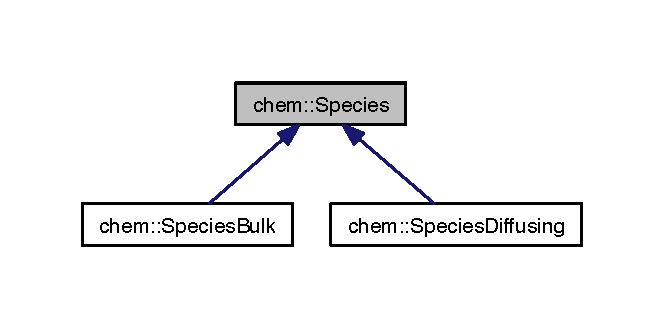
\includegraphics[width=319pt]{classchem_1_1Species__inherit__graph}
\end{center}
\end{figure}


Collaboration diagram for chem\-:\-:Species\-:\nopagebreak
\begin{figure}[H]
\begin{center}
\leavevmode
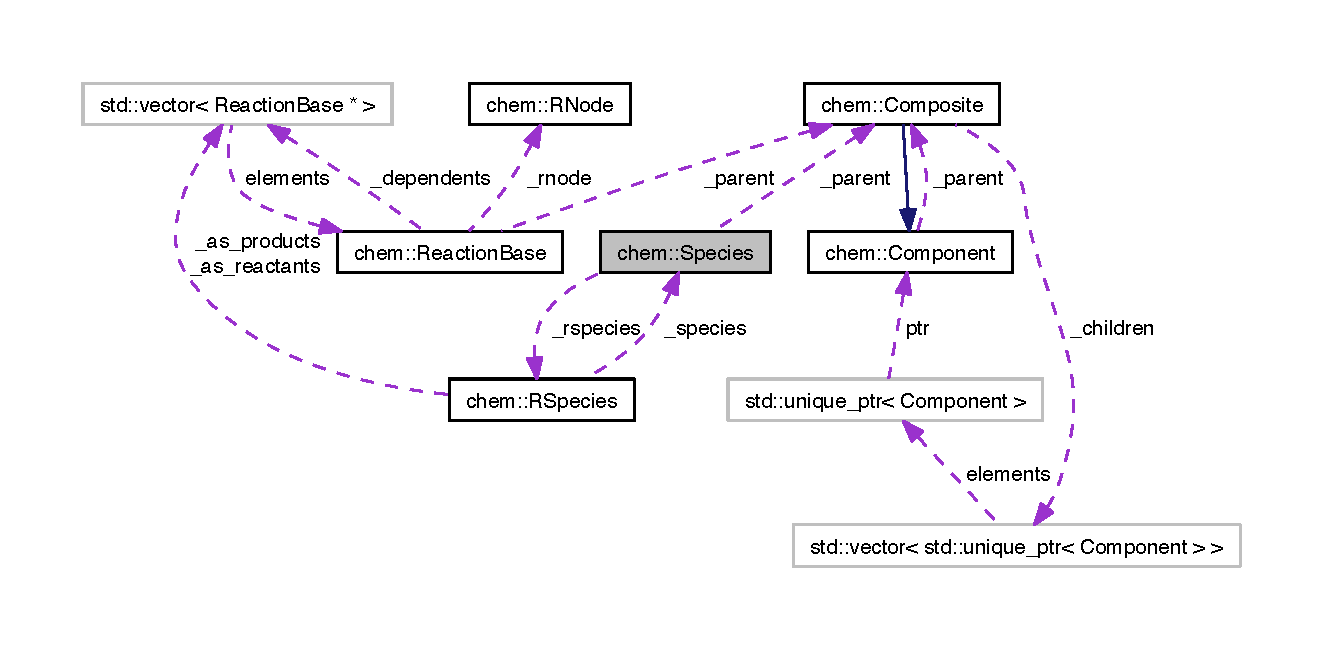
\includegraphics[width=350pt]{classchem_1_1Species__coll__graph}
\end{center}
\end{figure}
\subsection*{Public Member Functions}
\begin{DoxyCompactItemize}
\item 
\hyperlink{classchem_1_1Species_a979ab4590bae72bf0a413b930212340d}{Species} ()
\begin{DoxyCompactList}\small\item\em Default Constructor; Should not be used by the end users -\/ only internally (although it is not marked as private) \end{DoxyCompactList}\item 
\hyperlink{classchem_1_1Species_a2d67fe2e075842ed5877143f5771f51b}{Species} (const std\-::string \&name, \hyperlink{common_8h_a3503f321fd36304ee274141275cca586}{species\-\_\-copy\-\_\-t} n=0, \hyperlink{common_8h_a3503f321fd36304ee274141275cca586}{species\-\_\-copy\-\_\-t} ulim=\hyperlink{common_8h_adaf831a0b61083f29adf8fc6e8edab35}{max\-\_\-ulim})
\begin{DoxyCompactList}\small\item\em The constructor for this base class of \hyperlink{classchem_1_1Species}{Species} should not be called directly -\/ only by the concrete subclasses. \end{DoxyCompactList}\item 
\hyperlink{classchem_1_1Species_a785e10df4d7bc79b69a254f6cd296678}{Species} (const \hyperlink{classchem_1_1Species}{Species} \&rhs)
\begin{DoxyCompactList}\small\item\em Copy constructor. \end{DoxyCompactList}\item 
\hyperlink{classchem_1_1Species_a4a2af0ad2237d60a579e53c0410a8627}{Species} (\hyperlink{classchem_1_1Species}{Species} \&\&rhs) noexcept
\begin{DoxyCompactList}\small\item\em Move constructor -\/ makes it possible to easily add \hyperlink{classchem_1_1Species}{Species} to S\-T\-L containers, such as vector$<$\-Species$>$ One has to be careful with vector$<$\-Species$>$ as opposed to vector$<$\-Species$\ast$$>$. \end{DoxyCompactList}\item 
\hyperlink{classchem_1_1Species}{Species} \& \hyperlink{classchem_1_1Species_ae885477a490e183f1981cf2591cdbee8}{operator=} (const \hyperlink{classchem_1_1Species}{Species} \&rhs)
\begin{DoxyCompactList}\small\item\em Assignment operator An assignment A = B copies the name of B to A. \end{DoxyCompactList}\item 
\hyperlink{classchem_1_1Species}{Species} \& \hyperlink{classchem_1_1Species_ae9344aa4bcd5fb1a511361bef72162f6}{operator=} (\hyperlink{classchem_1_1Species}{Species} \&\&rhs)
\begin{DoxyCompactList}\small\item\em Move assignment is needed for the same reasons as move constructor. \end{DoxyCompactList}\item 
virtual \hyperlink{classchem_1_1Species}{Species} $\ast$ \hyperlink{classchem_1_1Species_acf0054a3704627698ba91293e8d0d370}{clone} ()
\item 
\hyperlink{classchem_1_1Composite}{Composite} $\ast$ \hyperlink{classchem_1_1Species_acdc83314b339310022d56e024f124a34}{get\-Parent} ()
\item 
void \hyperlink{classchem_1_1Species_a50e1e828d0b8a03efc9354e2c00174f5}{set\-Parent} (\hyperlink{classchem_1_1Composite}{Composite} $\ast$other)
\item 
bool \hyperlink{classchem_1_1Species_a6ddddc5be2b0e4427486f80a891879b3}{has\-Parent} () const 
\item 
\hyperlink{classchem_1_1Composite}{Composite} $\ast$ \hyperlink{classchem_1_1Species_aa5931e2aae4856c1b438691c23ada5aa}{get\-Root} ()
\item 
\hyperlink{classchem_1_1RSpecies}{R\-Species} \& \hyperlink{classchem_1_1Species_a1719a8155a69e9a62593d23d4bfc8514}{get\-R\-Species} ()
\begin{DoxyCompactList}\small\item\em Return a reference to \hyperlink{classchem_1_1RSpecies}{R\-Species}. \end{DoxyCompactList}\item 
const \hyperlink{classchem_1_1RSpecies}{R\-Species} \& \hyperlink{classchem_1_1Species_a438dae186317809effdd040ed38c568b}{get\-R\-Species} () const 
\begin{DoxyCompactList}\small\item\em Return a constant reference to \hyperlink{classchem_1_1RSpecies}{R\-Species}. \end{DoxyCompactList}\item 
void \hyperlink{classchem_1_1Species_af10a33a212fdb986fb93613e9c219f7a}{set\-N} (\hyperlink{common_8h_a3503f321fd36304ee274141275cca586}{species\-\_\-copy\-\_\-t} n)
\begin{DoxyCompactList}\small\item\em Sets the copy number for this \hyperlink{classchem_1_1Species}{Species}. \end{DoxyCompactList}\item 
\hyperlink{common_8h_a3503f321fd36304ee274141275cca586}{species\-\_\-copy\-\_\-t} \hyperlink{classchem_1_1Species_af7c9f51060b84169b428a7796dad6dca}{get\-N} () const 
\begin{DoxyCompactList}\small\item\em Return the current copy number of this \hyperlink{classchem_1_1Species}{Species}. \end{DoxyCompactList}\item 
\hyperlink{common_8h_a3503f321fd36304ee274141275cca586}{species\-\_\-copy\-\_\-t} \hyperlink{classchem_1_1Species_a05fbe0a05f028beb1bb729f19d44a56a}{get\-Upper\-Limit\-For\-N} () const 
\begin{DoxyCompactList}\small\item\em Return the upper limit for the copy number of this \hyperlink{classchem_1_1Species}{Species}. \end{DoxyCompactList}\item 
std\-::string \hyperlink{classchem_1_1Species_aa32c8f7fb344c68539a927c6a7f916c7}{get\-Name} () const 
\begin{DoxyCompactList}\small\item\em Return this \hyperlink{classchem_1_1Species}{Species}' name. \end{DoxyCompactList}\item 
int \hyperlink{classchem_1_1Species_a330ef4514a8979a6ea0e6f71ed5cb820}{get\-Molecule} () const 
\begin{DoxyCompactList}\small\item\em Return the molecule index associated with this \hyperlink{classchem_1_1Species}{Species}' (as int) \end{DoxyCompactList}\item 
bool \hyperlink{classchem_1_1Species_aa412f592e88600b48e3df591fc4cd655}{is\-Signaling} () const 
\begin{DoxyCompactList}\small\item\em Return true if this \hyperlink{classchem_1_1Species}{Species} emits signals on copy number change. \end{DoxyCompactList}\item 
void \hyperlink{classchem_1_1Species_a2d3d9f6e7c7d9c7bdd87ff5373a7d08c}{start\-Signaling} ()
\begin{DoxyCompactList}\small\item\em Set the signaling behavior of this \hyperlink{classchem_1_1Species}{Species} Gillespie-\/like simulation algorithm) \end{DoxyCompactList}\item 
void \hyperlink{classchem_1_1Species_a9d34195d05f3e35e00dd20892ff7393b}{stop\-Signaling} ()
\begin{DoxyCompactList}\small\item\em Destroy the signal associated with this \hyperlink{classchem_1_1Species}{Species}. \end{DoxyCompactList}\item 
boost\-::signals2\-::connection \hyperlink{classchem_1_1Species_a9a582e18e231a65761cb10c14d0a0a68}{connect} (std\-::function$<$ void(\hyperlink{classchem_1_1RSpecies}{R\-Species} $\ast$, int)$>$ const \&R\-Species\-\_\-callback, int priority=5)
\begin{DoxyCompactList}\small\item\em Connect the callback, rspecies\-\_\-callback to a signal corresponding to \hyperlink{classchem_1_1RSpecies}{R\-Species} $\ast$s. \end{DoxyCompactList}\item 
virtual \hyperlink{classchem_1_1Species_afb5803da12a3192f0c1b5bcbea4054d7}{$\sim$\-Species} () noexcept
\begin{DoxyCompactList}\small\item\em Virtual destructor. \end{DoxyCompactList}\item 
virtual std\-::string \hyperlink{classchem_1_1Species_a7ac7196a7146f63e297d0995c6081f4b}{get\-Full\-Name} () const 
\begin{DoxyCompactList}\small\item\em Return the full name of this \hyperlink{classchem_1_1Species}{Species} in a std\-::string format (e.\-g. \char`\"{}\-Arp2/3\{\-Bulk\}\char`\"{}. \end{DoxyCompactList}\item 
virtual size\-\_\-t \hyperlink{classchem_1_1Species_a5e8aedfe4c4b5e08fb0ee672c3d80ace}{count\-Species} () const 
\end{DoxyCompactItemize}
\subsection*{Private Attributes}
\begin{DoxyCompactItemize}
\item 
int \hyperlink{classchem_1_1Species_afc69264ab4c24ac17b7d1946b1b380f4}{\-\_\-molecule}
\begin{DoxyCompactList}\small\item\em unique id identifying the molecule (e.\-g. the integer id corresponding to \char`\"{}\-Arp2/3\char`\"{}) \end{DoxyCompactList}\item 
\hyperlink{classchem_1_1RSpecies}{R\-Species} $\ast$ \hyperlink{classchem_1_1Species_aa6a2ec40f6f1b08c76a184d11571c570}{\-\_\-rspecies}
\begin{DoxyCompactList}\small\item\em pointer to \hyperlink{classchem_1_1RSpecies}{R\-Species}; \hyperlink{classchem_1_1Species}{Species} is responsible for creating and destroying \hyperlink{classchem_1_1RSpecies}{R\-Species} \end{DoxyCompactList}\item 
\hyperlink{classchem_1_1Composite}{Composite} $\ast$ \hyperlink{classchem_1_1Species_ae0743ec422b63dcb29b4cbfee484902d}{\-\_\-parent}
\begin{DoxyCompactList}\small\item\em pointer to the \char`\"{}container\char`\"{} object holding this \hyperlink{classchem_1_1Species}{Species} (could be a nullptr) \end{DoxyCompactList}\end{DoxyCompactItemize}
\subsection*{Friends}
\begin{DoxyCompactItemize}
\item 
bool \hyperlink{classchem_1_1Species_a22987c5719b74c50465256ea5b9d80bf}{operator==} (const \hyperlink{classchem_1_1Species}{Species} \&a, const \hyperlink{classchem_1_1Species}{Species} \&b)
\begin{DoxyCompactList}\small\item\em Returns true if two \hyperlink{classchem_1_1Species}{Species} objects are equal. \end{DoxyCompactList}\item 
bool \hyperlink{classchem_1_1Species_aff630d716711fbbab3bc7f598230316b}{operator!=} (const \hyperlink{classchem_1_1Species}{Species} \&a, const \hyperlink{classchem_1_1Species}{Species} \&b)
\begin{DoxyCompactList}\small\item\em Return true if two \hyperlink{classchem_1_1Species}{Species} are not equal. \end{DoxyCompactList}\end{DoxyCompactItemize}


\subsection{Detailed Description}
\hyperlink{classchem_1_1Species}{Species} class represents chemical molecules, tracks their copy number and can be used in \hyperlink{classchem_1_1Reaction}{Reactions}. 

This class represents chemical species, such as G-\/\-Actin. As a class, it provides \hyperlink{classchem_1_1Species}{Species}' name, the current copy number of molecules, \hyperlink{classchem_1_1Species}{Species} type (e.\-g. S\-Type\-::\-Bulk), and a few other characteristics of a \hyperlink{classchem_1_1Species}{Species}. This class is synergetic with the \hyperlink{classchem_1_1Reaction}{Reaction}, since \hyperlink{classchem_1_1Species}{Species} can be added to \hyperlink{classchem_1_1Reaction}{Reactions}.

As a type, \hyperlink{classchem_1_1Species}{Species} is composed of the following primary fields\-: type, name, copy number. A subclass may added additional primary fields. Two \hyperlink{classchem_1_1Species}{Species} are mathematically equal, if their primary fields are equal. This means that applying the copy constructor will guarantee that primary fields will be equal\-: 
\begin{DoxyCode}
  SpeciesBulk A{"Arp2/3",25};
  SpeciesBulk B(A);
  assert(A==B); // A must be equal to B
\end{DoxyCode}


\begin{DoxyNote}{Note}
Each \hyperlink{classchem_1_1Species}{Species} owns an unshared \hyperlink{classchem_1_1RSpecies}{R\-Species} object. However, the \hyperlink{classchem_1_1RSpecies}{R\-Species} field is not among the primary fields defining the \hyperlink{classchem_1_1Species}{Species} identity (hence, the equality operator). In particular, upon copying, the source and target \hyperlink{classchem_1_1Species}{Species} will have distinct \hyperlink{classchem_1_1RSpecies}{R\-Species} fields. However, in a fully constructed program, the source and target species (after applying the copy constructor) should eventually be involved in the same set of equivalent reactions. This means that their respective reactions will return true when the equlaity operator is applied.

The \hyperlink{classchem_1_1Species}{Species} class allows callbacks (see make\-Signaling and related methods). 
\end{DoxyNote}


Definition at line 114 of file Species.\-h.



\subsection{Constructor \& Destructor Documentation}
\hypertarget{classchem_1_1Species_a979ab4590bae72bf0a413b930212340d}{\index{chem\-::\-Species@{chem\-::\-Species}!Species@{Species}}
\index{Species@{Species}!chem::Species@{chem\-::\-Species}}
\subsubsection[{Species}]{\setlength{\rightskip}{0pt plus 5cm}{\bf chem\-::\-Species\-::\-Species} (
\begin{DoxyParamCaption}
{}
\end{DoxyParamCaption}
)\hspace{0.3cm}{\ttfamily  \mbox{[}inline\mbox{]}}}}\label{classchem_1_1Species_a979ab4590bae72bf0a413b930212340d}


Default Constructor; Should not be used by the end users -\/ only internally (although it is not marked as private) 



Definition at line 121 of file Species.\-h.



References \-\_\-molecule, \-\_\-rspecies, chem\-::\-Species\-Names\-D\-B\-::\-Instance(), and chem\-::\-Species\-Names\-D\-B\-::string\-To\-Int().



Referenced by clone().

\hypertarget{classchem_1_1Species_a2d67fe2e075842ed5877143f5771f51b}{\index{chem\-::\-Species@{chem\-::\-Species}!Species@{Species}}
\index{Species@{Species}!chem::Species@{chem\-::\-Species}}
\subsubsection[{Species}]{\setlength{\rightskip}{0pt plus 5cm}{\bf chem\-::\-Species\-::\-Species} (
\begin{DoxyParamCaption}
\item[{const std\-::string \&}]{name, }
\item[{{\bf species\-\_\-copy\-\_\-t}}]{n = {\ttfamily 0}, }
\item[{{\bf species\-\_\-copy\-\_\-t}}]{ulim = {\ttfamily {\bf max\-\_\-ulim}}}
\end{DoxyParamCaption}
)\hspace{0.3cm}{\ttfamily  \mbox{[}inline\mbox{]}}}}\label{classchem_1_1Species_a2d67fe2e075842ed5877143f5771f51b}


The constructor for this base class of \hyperlink{classchem_1_1Species}{Species} should not be called directly -\/ only by the concrete subclasses. 


\begin{DoxyParams}{Parameters}
{\em name} & -\/ a string for the \hyperlink{classchem_1_1Species}{Species} name associated with this \hyperlink{classchem_1_1Species}{Species}. For example, \char`\"{}\-G-\/\-Actin\char`\"{} or \char`\"{}\-Arp2/3\char`\"{} \\
\hline
{\em type\-\_\-enum} & -\/ S\-Type enum, such as S\-Type\-::\-Diffusing \\
\hline
{\em n} & -\/ copy number \\
\hline
{\em ulim} & -\/ upper limit for this species' copy number \\
\hline
\end{DoxyParams}


Definition at line 132 of file Species.\-h.



References \-\_\-molecule, \-\_\-rspecies, chem\-::\-Species\-Names\-D\-B\-::\-Instance(), and chem\-::\-Species\-Names\-D\-B\-::string\-To\-Int().

\hypertarget{classchem_1_1Species_a785e10df4d7bc79b69a254f6cd296678}{\index{chem\-::\-Species@{chem\-::\-Species}!Species@{Species}}
\index{Species@{Species}!chem::Species@{chem\-::\-Species}}
\subsubsection[{Species}]{\setlength{\rightskip}{0pt plus 5cm}{\bf chem\-::\-Species\-::\-Species} (
\begin{DoxyParamCaption}
\item[{const {\bf Species} \&}]{rhs}
\end{DoxyParamCaption}
)\hspace{0.3cm}{\ttfamily  \mbox{[}inline\mbox{]}}}}\label{classchem_1_1Species_a785e10df4d7bc79b69a254f6cd296678}


Copy constructor. 

\begin{DoxyNote}{Note}
The associated \hyperlink{classchem_1_1RSpecies}{R\-Species} subpart is not copied, but a new one is created. This means that the copied destination \hyperlink{classchem_1_1Species}{Species} won't be included in any \hyperlink{classchem_1_1Reaction}{Reaction} interactions of the original source \hyperlink{classchem_1_1Species}{Species}. The species copy numbered is copied to the target. The A \hyperlink{classchem_1_1Species}{Species} parent attriute is not copied, but set to nullptr. 
\end{DoxyNote}


Definition at line 145 of file Species.\-h.



References \-\_\-rspecies, get\-N(), and get\-Upper\-Limit\-For\-N().

\hypertarget{classchem_1_1Species_a4a2af0ad2237d60a579e53c0410a8627}{\index{chem\-::\-Species@{chem\-::\-Species}!Species@{Species}}
\index{Species@{Species}!chem::Species@{chem\-::\-Species}}
\subsubsection[{Species}]{\setlength{\rightskip}{0pt plus 5cm}{\bf chem\-::\-Species\-::\-Species} (
\begin{DoxyParamCaption}
\item[{{\bf Species} \&\&}]{rhs}
\end{DoxyParamCaption}
)\hspace{0.3cm}{\ttfamily  \mbox{[}inline\mbox{]}}}}\label{classchem_1_1Species_a4a2af0ad2237d60a579e53c0410a8627}


Move constructor -\/ makes it possible to easily add \hyperlink{classchem_1_1Species}{Species} to S\-T\-L containers, such as vector$<$\-Species$>$ One has to be careful with vector$<$\-Species$>$ as opposed to vector$<$\-Species$\ast$$>$. 

The latter is \char`\"{}safe\char`\"{} in terms of being internally moved around by vector.\-resize, etc., but vector$<$\-Species$>$ would copy \hyperlink{classchem_1_1Species}{Species} if a move constructor is not available. This will then destruct the original \hyperlink{classchem_1_1Species}{Species} (with its associated \hyperlink{classchem_1_1RSpecies}{R\-Species}), hence, the \hyperlink{classchem_1_1Reaction}{Reaction} network of the \hyperlink{classchem_1_1Species}{Species} will be lost. Since this behavior is most likely not desired or unacceptable, the internal vector operations should only \char`\"{}move\char`\"{} the \hyperlink{classchem_1_1Species}{Species} around, without copying. Moving transfers the \hyperlink{classchem_1_1RSpecies}{R\-Species} pointer from source to target, stealing resources from the source, leaving it for destruction. The \hyperlink{classchem_1_1Species}{Species} parent attriute is moved it. 

Definition at line 162 of file Species.\-h.

\hypertarget{classchem_1_1Species_afb5803da12a3192f0c1b5bcbea4054d7}{\index{chem\-::\-Species@{chem\-::\-Species}!$\sim$\-Species@{$\sim$\-Species}}
\index{$\sim$\-Species@{$\sim$\-Species}!chem::Species@{chem\-::\-Species}}
\subsubsection[{$\sim$\-Species}]{\setlength{\rightskip}{0pt plus 5cm}virtual {\bf chem\-::\-Species\-::$\sim$\-Species} (
\begin{DoxyParamCaption}
{}
\end{DoxyParamCaption}
)\hspace{0.3cm}{\ttfamily  \mbox{[}inline, virtual\mbox{]}}}}\label{classchem_1_1Species_afb5803da12a3192f0c1b5bcbea4054d7}


Virtual destructor. 

\begin{DoxyNote}{Note}
noexcept is important here. Otherwise, gcc flags the constructor as potentially throwing, which in turn disables move operations by the S\-T\-L containers. This behaviour is a gcc bug (as of gcc 4.\-703), and will presumbaly be fixed in the future. 
\end{DoxyNote}


Definition at line 276 of file Species.\-h.



References \-\_\-rspecies.



\subsection{Member Function Documentation}
\hypertarget{classchem_1_1Species_acf0054a3704627698ba91293e8d0d370}{\index{chem\-::\-Species@{chem\-::\-Species}!clone@{clone}}
\index{clone@{clone}!chem::Species@{chem\-::\-Species}}
\subsubsection[{clone}]{\setlength{\rightskip}{0pt plus 5cm}virtual {\bf Species}$\ast$ {\bf chem\-::\-Species\-::clone} (
\begin{DoxyParamCaption}
{}
\end{DoxyParamCaption}
)\hspace{0.3cm}{\ttfamily  \mbox{[}inline, virtual\mbox{]}}}}\label{classchem_1_1Species_acf0054a3704627698ba91293e8d0d370}


Reimplemented in \hyperlink{classchem_1_1SpeciesDiffusing_a69edbe33378230389a2fb99c4ca2b5ce}{chem\-::\-Species\-Diffusing}, and \hyperlink{classchem_1_1SpeciesBulk_a7bfdd13273d7328c2f7d275796e57873}{chem\-::\-Species\-Bulk}.



Definition at line 195 of file Species.\-h.



References Species().

\hypertarget{classchem_1_1Species_a9a582e18e231a65761cb10c14d0a0a68}{\index{chem\-::\-Species@{chem\-::\-Species}!connect@{connect}}
\index{connect@{connect}!chem::Species@{chem\-::\-Species}}
\subsubsection[{connect}]{\setlength{\rightskip}{0pt plus 5cm}boost\-::signals2\-::connection {\bf chem\-::\-Species\-::connect} (
\begin{DoxyParamCaption}
\item[{std\-::function$<$ void({\bf R\-Species} $\ast$, int)$>$ const \&}]{R\-Species\-\_\-callback, }
\item[{int}]{priority = {\ttfamily 5}}
\end{DoxyParamCaption}
)}}\label{classchem_1_1Species_a9a582e18e231a65761cb10c14d0a0a68}


Connect the callback, rspecies\-\_\-callback to a signal corresponding to \hyperlink{classchem_1_1RSpecies}{R\-Species} $\ast$s. 


\begin{DoxyParams}{Parameters}
{\em std\-::function$<$void} & (\hyperlink{classchem_1_1RSpecies}{R\-Species} $\ast$, int)$>$ const \&R\-Species\-\_\-callback -\/ a function object to be called (a slot) \\
\hline
{\em int} & priority -\/ lower priority slots will be called first. Default is 5 Do not use priorities 1 and 2 unless absolutely essential. \\
\hline
\end{DoxyParams}
\begin{DoxyReturn}{Returns}
a connection object which can be used to later disconnect this particular slot or temporarily block it 
\end{DoxyReturn}


Definition at line 27 of file Species.\-cpp.



References \-\_\-rspecies, chem\-::\-R\-Species\-::\-\_\-signal, is\-Signaling(), and start\-Signaling().

\hypertarget{classchem_1_1Species_a5e8aedfe4c4b5e08fb0ee672c3d80ace}{\index{chem\-::\-Species@{chem\-::\-Species}!count\-Species@{count\-Species}}
\index{count\-Species@{count\-Species}!chem::Species@{chem\-::\-Species}}
\subsubsection[{count\-Species}]{\setlength{\rightskip}{0pt plus 5cm}virtual size\-\_\-t {\bf chem\-::\-Species\-::count\-Species} (
\begin{DoxyParamCaption}
{}
\end{DoxyParamCaption}
) const\hspace{0.3cm}{\ttfamily  \mbox{[}inline, virtual\mbox{]}}}}\label{classchem_1_1Species_a5e8aedfe4c4b5e08fb0ee672c3d80ace}


Definition at line 285 of file Species.\-h.

\hypertarget{classchem_1_1Species_a7ac7196a7146f63e297d0995c6081f4b}{\index{chem\-::\-Species@{chem\-::\-Species}!get\-Full\-Name@{get\-Full\-Name}}
\index{get\-Full\-Name@{get\-Full\-Name}!chem::Species@{chem\-::\-Species}}
\subsubsection[{get\-Full\-Name}]{\setlength{\rightskip}{0pt plus 5cm}virtual std\-::string {\bf chem\-::\-Species\-::get\-Full\-Name} (
\begin{DoxyParamCaption}
{}
\end{DoxyParamCaption}
) const\hspace{0.3cm}{\ttfamily  \mbox{[}inline, virtual\mbox{]}}}}\label{classchem_1_1Species_a7ac7196a7146f63e297d0995c6081f4b}


Return the full name of this \hyperlink{classchem_1_1Species}{Species} in a std\-::string format (e.\-g. \char`\"{}\-Arp2/3\{\-Bulk\}\char`\"{}. 



Reimplemented in \hyperlink{classchem_1_1SpeciesDiffusing_a03eba31a17a3713e8c45cc0952e922bb}{chem\-::\-Species\-Diffusing}, and \hyperlink{classchem_1_1SpeciesBulk_a340d3f16e075352bf1cbab7918f5ca20}{chem\-::\-Species\-Bulk}.



Definition at line 283 of file Species.\-h.



References get\-Name().



Referenced by operator$<$$<$().

\hypertarget{classchem_1_1Species_a330ef4514a8979a6ea0e6f71ed5cb820}{\index{chem\-::\-Species@{chem\-::\-Species}!get\-Molecule@{get\-Molecule}}
\index{get\-Molecule@{get\-Molecule}!chem::Species@{chem\-::\-Species}}
\subsubsection[{get\-Molecule}]{\setlength{\rightskip}{0pt plus 5cm}int {\bf chem\-::\-Species\-::get\-Molecule} (
\begin{DoxyParamCaption}
{}
\end{DoxyParamCaption}
) const\hspace{0.3cm}{\ttfamily  \mbox{[}inline\mbox{]}}}}\label{classchem_1_1Species_a330ef4514a8979a6ea0e6f71ed5cb820}


Return the molecule index associated with this \hyperlink{classchem_1_1Species}{Species}' (as int) 



Definition at line 231 of file Species.\-h.



References \-\_\-molecule.



Referenced by chem\-::\-Compartment\-::add\-Species(), chem\-::\-Compartment\-::add\-Species\-Unique(), and chem\-::\-Compartment\-::set\-Diffusion\-Rate().

\hypertarget{classchem_1_1Species_af7c9f51060b84169b428a7796dad6dca}{\index{chem\-::\-Species@{chem\-::\-Species}!get\-N@{get\-N}}
\index{get\-N@{get\-N}!chem::Species@{chem\-::\-Species}}
\subsubsection[{get\-N}]{\setlength{\rightskip}{0pt plus 5cm}{\bf species\-\_\-copy\-\_\-t} {\bf chem\-::\-Species\-::get\-N} (
\begin{DoxyParamCaption}
{}
\end{DoxyParamCaption}
) const\hspace{0.3cm}{\ttfamily  \mbox{[}inline\mbox{]}}}}\label{classchem_1_1Species_af7c9f51060b84169b428a7796dad6dca}


Return the current copy number of this \hyperlink{classchem_1_1Species}{Species}. 



Definition at line 220 of file Species.\-h.



References \-\_\-rspecies, and chem\-::\-R\-Species\-::get\-N().



Referenced by operator$<$$<$(), operator=(), and Species().

\hypertarget{classchem_1_1Species_aa32c8f7fb344c68539a927c6a7f916c7}{\index{chem\-::\-Species@{chem\-::\-Species}!get\-Name@{get\-Name}}
\index{get\-Name@{get\-Name}!chem::Species@{chem\-::\-Species}}
\subsubsection[{get\-Name}]{\setlength{\rightskip}{0pt plus 5cm}std\-::string {\bf chem\-::\-Species\-::get\-Name} (
\begin{DoxyParamCaption}
{}
\end{DoxyParamCaption}
) const\hspace{0.3cm}{\ttfamily  \mbox{[}inline\mbox{]}}}}\label{classchem_1_1Species_aa32c8f7fb344c68539a927c6a7f916c7}


Return this \hyperlink{classchem_1_1Species}{Species}' name. 



Definition at line 228 of file Species.\-h.



References \-\_\-molecule, chem\-::\-Species\-Names\-D\-B\-::\-Instance(), and chem\-::\-Species\-Names\-D\-B\-::int\-To\-String().



Referenced by get\-Full\-Name(), chem\-::\-Species\-Bulk\-::get\-Full\-Name(), and chem\-::\-Species\-Diffusing\-::get\-Full\-Name().

\hypertarget{classchem_1_1Species_acdc83314b339310022d56e024f124a34}{\index{chem\-::\-Species@{chem\-::\-Species}!get\-Parent@{get\-Parent}}
\index{get\-Parent@{get\-Parent}!chem::Species@{chem\-::\-Species}}
\subsubsection[{get\-Parent}]{\setlength{\rightskip}{0pt plus 5cm}{\bf Composite}$\ast$ {\bf chem\-::\-Species\-::get\-Parent} (
\begin{DoxyParamCaption}
{}
\end{DoxyParamCaption}
)\hspace{0.3cm}{\ttfamily  \mbox{[}inline\mbox{]}}}}\label{classchem_1_1Species_acdc83314b339310022d56e024f124a34}


Definition at line 199 of file Species.\-h.



References \-\_\-parent.



Referenced by get\-Root().

\hypertarget{classchem_1_1Species_aa5931e2aae4856c1b438691c23ada5aa}{\index{chem\-::\-Species@{chem\-::\-Species}!get\-Root@{get\-Root}}
\index{get\-Root@{get\-Root}!chem::Species@{chem\-::\-Species}}
\subsubsection[{get\-Root}]{\setlength{\rightskip}{0pt plus 5cm}{\bf Composite} $\ast$ {\bf chem\-::\-Species\-::get\-Root} (
\begin{DoxyParamCaption}
{}
\end{DoxyParamCaption}
)}}\label{classchem_1_1Species_aa5931e2aae4856c1b438691c23ada5aa}


Definition at line 35 of file Species.\-cpp.



References get\-Parent(), chem\-::\-Component\-::get\-Root(), and has\-Parent().

\hypertarget{classchem_1_1Species_a1719a8155a69e9a62593d23d4bfc8514}{\index{chem\-::\-Species@{chem\-::\-Species}!get\-R\-Species@{get\-R\-Species}}
\index{get\-R\-Species@{get\-R\-Species}!chem::Species@{chem\-::\-Species}}
\subsubsection[{get\-R\-Species}]{\setlength{\rightskip}{0pt plus 5cm}{\bf R\-Species}\& {\bf chem\-::\-Species\-::get\-R\-Species} (
\begin{DoxyParamCaption}
{}
\end{DoxyParamCaption}
)\hspace{0.3cm}{\ttfamily  \mbox{[}inline\mbox{]}}}}\label{classchem_1_1Species_a1719a8155a69e9a62593d23d4bfc8514}


Return a reference to \hyperlink{classchem_1_1RSpecies}{R\-Species}. 

Notice that value copying won't be allowed because \hyperlink{classchem_1_1RSpecies}{R\-Species} is not copyable. 

Definition at line 209 of file Species.\-h.



References \-\_\-rspecies.



Referenced by chem\-::\-Chem\-Signal\-::connect(), and main().

\hypertarget{classchem_1_1Species_a438dae186317809effdd040ed38c568b}{\index{chem\-::\-Species@{chem\-::\-Species}!get\-R\-Species@{get\-R\-Species}}
\index{get\-R\-Species@{get\-R\-Species}!chem::Species@{chem\-::\-Species}}
\subsubsection[{get\-R\-Species}]{\setlength{\rightskip}{0pt plus 5cm}const {\bf R\-Species}\& {\bf chem\-::\-Species\-::get\-R\-Species} (
\begin{DoxyParamCaption}
{}
\end{DoxyParamCaption}
) const\hspace{0.3cm}{\ttfamily  \mbox{[}inline\mbox{]}}}}\label{classchem_1_1Species_a438dae186317809effdd040ed38c568b}


Return a constant reference to \hyperlink{classchem_1_1RSpecies}{R\-Species}. 



Definition at line 212 of file Species.\-h.



References \-\_\-rspecies.

\hypertarget{classchem_1_1Species_a05fbe0a05f028beb1bb729f19d44a56a}{\index{chem\-::\-Species@{chem\-::\-Species}!get\-Upper\-Limit\-For\-N@{get\-Upper\-Limit\-For\-N}}
\index{get\-Upper\-Limit\-For\-N@{get\-Upper\-Limit\-For\-N}!chem::Species@{chem\-::\-Species}}
\subsubsection[{get\-Upper\-Limit\-For\-N}]{\setlength{\rightskip}{0pt plus 5cm}{\bf species\-\_\-copy\-\_\-t} {\bf chem\-::\-Species\-::get\-Upper\-Limit\-For\-N} (
\begin{DoxyParamCaption}
{}
\end{DoxyParamCaption}
) const\hspace{0.3cm}{\ttfamily  \mbox{[}inline\mbox{]}}}}\label{classchem_1_1Species_a05fbe0a05f028beb1bb729f19d44a56a}


Return the upper limit for the copy number of this \hyperlink{classchem_1_1Species}{Species}. 



Definition at line 224 of file Species.\-h.



References \-\_\-rspecies, and chem\-::\-R\-Species\-::get\-Upper\-Limit\-For\-N().



Referenced by operator=(), and Species().

\hypertarget{classchem_1_1Species_a6ddddc5be2b0e4427486f80a891879b3}{\index{chem\-::\-Species@{chem\-::\-Species}!has\-Parent@{has\-Parent}}
\index{has\-Parent@{has\-Parent}!chem::Species@{chem\-::\-Species}}
\subsubsection[{has\-Parent}]{\setlength{\rightskip}{0pt plus 5cm}bool {\bf chem\-::\-Species\-::has\-Parent} (
\begin{DoxyParamCaption}
{}
\end{DoxyParamCaption}
) const\hspace{0.3cm}{\ttfamily  \mbox{[}inline\mbox{]}}}}\label{classchem_1_1Species_a6ddddc5be2b0e4427486f80a891879b3}


Definition at line 203 of file Species.\-h.



References \-\_\-parent.



Referenced by get\-Root().

\hypertarget{classchem_1_1Species_aa412f592e88600b48e3df591fc4cd655}{\index{chem\-::\-Species@{chem\-::\-Species}!is\-Signaling@{is\-Signaling}}
\index{is\-Signaling@{is\-Signaling}!chem::Species@{chem\-::\-Species}}
\subsubsection[{is\-Signaling}]{\setlength{\rightskip}{0pt plus 5cm}bool {\bf chem\-::\-Species\-::is\-Signaling} (
\begin{DoxyParamCaption}
{}
\end{DoxyParamCaption}
) const\hspace{0.3cm}{\ttfamily  \mbox{[}inline\mbox{]}}}}\label{classchem_1_1Species_aa412f592e88600b48e3df591fc4cd655}


Return true if this \hyperlink{classchem_1_1Species}{Species} emits signals on copy number change. 



Definition at line 235 of file Species.\-h.



References \-\_\-rspecies, and chem\-::\-R\-Species\-::is\-Signaling().



Referenced by connect().

\hypertarget{classchem_1_1Species_ae885477a490e183f1981cf2591cdbee8}{\index{chem\-::\-Species@{chem\-::\-Species}!operator=@{operator=}}
\index{operator=@{operator=}!chem::Species@{chem\-::\-Species}}
\subsubsection[{operator=}]{\setlength{\rightskip}{0pt plus 5cm}{\bf Species}\& chem\-::\-Species\-::operator= (
\begin{DoxyParamCaption}
\item[{const {\bf Species} \&}]{rhs}
\end{DoxyParamCaption}
)\hspace{0.3cm}{\ttfamily  \mbox{[}inline\mbox{]}}}}\label{classchem_1_1Species_ae885477a490e183f1981cf2591cdbee8}


Assignment operator An assignment A = B copies the name of B to A. 

It destroys the \hyperlink{classchem_1_1Reaction}{Reaction} interactions of A, and resents them to a blank value (i.\-e. A won't be involced in any Reactions). B's \hyperlink{classchem_1_1Reaction}{Reaction} interactions are not copied. The copy number of B is copied to A. The A \hyperlink{classchem_1_1Species}{Species} parent attriute is not copied, but set to nullptr. 

Definition at line 172 of file Species.\-h.



References \-\_\-molecule, \-\_\-parent, \-\_\-rspecies, get\-N(), and get\-Upper\-Limit\-For\-N().

\hypertarget{classchem_1_1Species_ae9344aa4bcd5fb1a511361bef72162f6}{\index{chem\-::\-Species@{chem\-::\-Species}!operator=@{operator=}}
\index{operator=@{operator=}!chem::Species@{chem\-::\-Species}}
\subsubsection[{operator=}]{\setlength{\rightskip}{0pt plus 5cm}{\bf Species}\& chem\-::\-Species\-::operator= (
\begin{DoxyParamCaption}
\item[{{\bf Species} \&\&}]{rhs}
\end{DoxyParamCaption}
)\hspace{0.3cm}{\ttfamily  \mbox{[}inline\mbox{]}}}}\label{classchem_1_1Species_ae9344aa4bcd5fb1a511361bef72162f6}


Move assignment is needed for the same reasons as move constructor. 

\begin{DoxySeeAlso}{See also}
\hyperlink{classchem_1_1Species}{Species} (\hyperlink{classchem_1_1Species}{Species} \&\&rhs) 
\end{DoxySeeAlso}


Definition at line 186 of file Species.\-h.



References \-\_\-molecule, \-\_\-parent, and \-\_\-rspecies.

\hypertarget{classchem_1_1Species_af10a33a212fdb986fb93613e9c219f7a}{\index{chem\-::\-Species@{chem\-::\-Species}!set\-N@{set\-N}}
\index{set\-N@{set\-N}!chem::Species@{chem\-::\-Species}}
\subsubsection[{set\-N}]{\setlength{\rightskip}{0pt plus 5cm}void {\bf chem\-::\-Species\-::set\-N} (
\begin{DoxyParamCaption}
\item[{{\bf species\-\_\-copy\-\_\-t}}]{n}
\end{DoxyParamCaption}
)\hspace{0.3cm}{\ttfamily  \mbox{[}inline\mbox{]}}}}\label{classchem_1_1Species_af10a33a212fdb986fb93613e9c219f7a}


Sets the copy number for this \hyperlink{classchem_1_1Species}{Species}. 


\begin{DoxyParams}{Parameters}
{\em n} & should be a non-\/negative number, but no checking is done in run time \\
\hline
\end{DoxyParams}
\begin{DoxyNote}{Note}
The operation does not emit any signals about the copy number change. 
\end{DoxyNote}


Definition at line 217 of file Species.\-h.



References \-\_\-rspecies, and chem\-::\-R\-Species\-::set\-N().



Referenced by main().

\hypertarget{classchem_1_1Species_a50e1e828d0b8a03efc9354e2c00174f5}{\index{chem\-::\-Species@{chem\-::\-Species}!set\-Parent@{set\-Parent}}
\index{set\-Parent@{set\-Parent}!chem::Species@{chem\-::\-Species}}
\subsubsection[{set\-Parent}]{\setlength{\rightskip}{0pt plus 5cm}void {\bf chem\-::\-Species\-::set\-Parent} (
\begin{DoxyParamCaption}
\item[{{\bf Composite} $\ast$}]{other}
\end{DoxyParamCaption}
)\hspace{0.3cm}{\ttfamily  \mbox{[}inline\mbox{]}}}}\label{classchem_1_1Species_a50e1e828d0b8a03efc9354e2c00174f5}


Definition at line 201 of file Species.\-h.



References \-\_\-parent.



Referenced by chem\-::\-Compartment\-::add\-Species(), and chem\-::\-Compartment\-::add\-Species\-Unique().

\hypertarget{classchem_1_1Species_a2d3d9f6e7c7d9c7bdd87ff5373a7d08c}{\index{chem\-::\-Species@{chem\-::\-Species}!start\-Signaling@{start\-Signaling}}
\index{start\-Signaling@{start\-Signaling}!chem::Species@{chem\-::\-Species}}
\subsubsection[{start\-Signaling}]{\setlength{\rightskip}{0pt plus 5cm}void {\bf chem\-::\-Species\-::start\-Signaling} (
\begin{DoxyParamCaption}
{}
\end{DoxyParamCaption}
)\hspace{0.3cm}{\ttfamily  \mbox{[}inline\mbox{]}}}}\label{classchem_1_1Species_a2d3d9f6e7c7d9c7bdd87ff5373a7d08c}


Set the signaling behavior of this \hyperlink{classchem_1_1Species}{Species} Gillespie-\/like simulation algorithm) 



Definition at line 239 of file Species.\-h.



References \-\_\-rspecies, and chem\-::\-R\-Species\-::start\-Signaling().



Referenced by connect().

\hypertarget{classchem_1_1Species_a9d34195d05f3e35e00dd20892ff7393b}{\index{chem\-::\-Species@{chem\-::\-Species}!stop\-Signaling@{stop\-Signaling}}
\index{stop\-Signaling@{stop\-Signaling}!chem::Species@{chem\-::\-Species}}
\subsubsection[{stop\-Signaling}]{\setlength{\rightskip}{0pt plus 5cm}void {\bf chem\-::\-Species\-::stop\-Signaling} (
\begin{DoxyParamCaption}
{}
\end{DoxyParamCaption}
)\hspace{0.3cm}{\ttfamily  \mbox{[}inline\mbox{]}}}}\label{classchem_1_1Species_a9d34195d05f3e35e00dd20892ff7393b}


Destroy the signal associated with this \hyperlink{classchem_1_1Species}{Species}. 

\begin{DoxyNote}{Note}
To start signaling again, make\-Signaling(...) needs to be called 
\end{DoxyNote}


Definition at line 243 of file Species.\-h.



References \-\_\-rspecies, and chem\-::\-R\-Species\-::stop\-Signaling().



\subsection{Friends And Related Function Documentation}
\hypertarget{classchem_1_1Species_aff630d716711fbbab3bc7f598230316b}{\index{chem\-::\-Species@{chem\-::\-Species}!operator!=@{operator!=}}
\index{operator!=@{operator!=}!chem::Species@{chem\-::\-Species}}
\subsubsection[{operator!=}]{\setlength{\rightskip}{0pt plus 5cm}bool operator!= (
\begin{DoxyParamCaption}
\item[{const {\bf Species} \&}]{a, }
\item[{const {\bf Species} \&}]{b}
\end{DoxyParamCaption}
)\hspace{0.3cm}{\ttfamily  \mbox{[}friend\mbox{]}}}}\label{classchem_1_1Species_aff630d716711fbbab3bc7f598230316b}


Return true if two \hyperlink{classchem_1_1Species}{Species} are not equal. 

\begin{DoxySeeAlso}{See also}
\hyperlink{classchem_1_1Species_a22987c5719b74c50465256ea5b9d80bf}{operator ==(const Species\& a, const Species\& b)} above 
\end{DoxySeeAlso}


Definition at line 266 of file Species.\-h.

\hypertarget{classchem_1_1Species_a22987c5719b74c50465256ea5b9d80bf}{\index{chem\-::\-Species@{chem\-::\-Species}!operator==@{operator==}}
\index{operator==@{operator==}!chem::Species@{chem\-::\-Species}}
\subsubsection[{operator==}]{\setlength{\rightskip}{0pt plus 5cm}bool operator== (
\begin{DoxyParamCaption}
\item[{const {\bf Species} \&}]{a, }
\item[{const {\bf Species} \&}]{b}
\end{DoxyParamCaption}
)\hspace{0.3cm}{\ttfamily  \mbox{[}friend\mbox{]}}}}\label{classchem_1_1Species_a22987c5719b74c50465256ea5b9d80bf}


Returns true if two \hyperlink{classchem_1_1Species}{Species} objects are equal. 

This function would accept derived class of \hyperlink{classchem_1_1Species}{Species}, such as \hyperlink{classchem_1_1SpeciesBulk}{Species\-Bulk} Two \hyperlink{classchem_1_1Species}{Species} are equal if their S\-Type(s) are equal (i.\-e. are of the same class), their names are equal. 

Definition at line 257 of file Species.\-h.



\subsection{Member Data Documentation}
\hypertarget{classchem_1_1Species_afc69264ab4c24ac17b7d1946b1b380f4}{\index{chem\-::\-Species@{chem\-::\-Species}!\-\_\-molecule@{\-\_\-molecule}}
\index{\-\_\-molecule@{\-\_\-molecule}!chem::Species@{chem\-::\-Species}}
\subsubsection[{\-\_\-molecule}]{\setlength{\rightskip}{0pt plus 5cm}int {\bf chem\-::\-Species\-::\-\_\-molecule}\hspace{0.3cm}{\ttfamily  \mbox{[}private\mbox{]}}}}\label{classchem_1_1Species_afc69264ab4c24ac17b7d1946b1b380f4}


unique id identifying the molecule (e.\-g. the integer id corresponding to \char`\"{}\-Arp2/3\char`\"{}) 



Definition at line 116 of file Species.\-h.



Referenced by get\-Molecule(), get\-Name(), operator=(), and Species().

\hypertarget{classchem_1_1Species_ae0743ec422b63dcb29b4cbfee484902d}{\index{chem\-::\-Species@{chem\-::\-Species}!\-\_\-parent@{\-\_\-parent}}
\index{\-\_\-parent@{\-\_\-parent}!chem::Species@{chem\-::\-Species}}
\subsubsection[{\-\_\-parent}]{\setlength{\rightskip}{0pt plus 5cm}{\bf Composite}$\ast$ {\bf chem\-::\-Species\-::\-\_\-parent}\hspace{0.3cm}{\ttfamily  \mbox{[}private\mbox{]}}}}\label{classchem_1_1Species_ae0743ec422b63dcb29b4cbfee484902d}


pointer to the \char`\"{}container\char`\"{} object holding this \hyperlink{classchem_1_1Species}{Species} (could be a nullptr) 



Definition at line 118 of file Species.\-h.



Referenced by get\-Parent(), has\-Parent(), operator=(), and set\-Parent().

\hypertarget{classchem_1_1Species_aa6a2ec40f6f1b08c76a184d11571c570}{\index{chem\-::\-Species@{chem\-::\-Species}!\-\_\-rspecies@{\-\_\-rspecies}}
\index{\-\_\-rspecies@{\-\_\-rspecies}!chem::Species@{chem\-::\-Species}}
\subsubsection[{\-\_\-rspecies}]{\setlength{\rightskip}{0pt plus 5cm}{\bf R\-Species}$\ast$ {\bf chem\-::\-Species\-::\-\_\-rspecies}\hspace{0.3cm}{\ttfamily  \mbox{[}private\mbox{]}}}}\label{classchem_1_1Species_aa6a2ec40f6f1b08c76a184d11571c570}


pointer to \hyperlink{classchem_1_1RSpecies}{R\-Species}; \hyperlink{classchem_1_1Species}{Species} is responsible for creating and destroying \hyperlink{classchem_1_1RSpecies}{R\-Species} 



Definition at line 117 of file Species.\-h.



Referenced by connect(), get\-N(), get\-R\-Species(), get\-Upper\-Limit\-For\-N(), is\-Signaling(), operator=(), set\-N(), Species(), start\-Signaling(), stop\-Signaling(), and $\sim$\-Species().



The documentation for this class was generated from the following files\-:\begin{DoxyCompactItemize}
\item 
Cyto\-Sim/\hyperlink{Species_8h}{Species.\-h}\item 
Cyto\-Sim/\hyperlink{Species_8cpp}{Species.\-cpp}\end{DoxyCompactItemize}

\hypertarget{classchem_1_1SpeciesBulk}{\section{chem\-:\-:Species\-Bulk Class Reference}
\label{classchem_1_1SpeciesBulk}\index{chem\-::\-Species\-Bulk@{chem\-::\-Species\-Bulk}}
}


\hyperlink{classchem_1_1SpeciesBulk}{Species\-Bulk} should be used for \hyperlink{classchem_1_1Species}{Species} without spatial information (i.\-e. well-\/mixed in the container)  




{\ttfamily \#include $<$Species.\-h$>$}



Inheritance diagram for chem\-:\-:Species\-Bulk\-:
\nopagebreak
\begin{figure}[H]
\begin{center}
\leavevmode
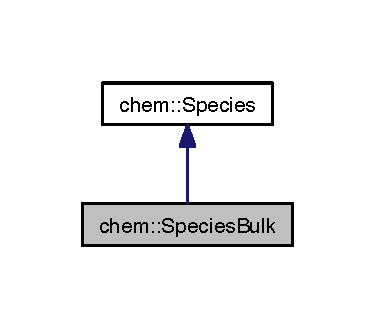
\includegraphics[width=176pt]{classchem_1_1SpeciesBulk__inherit__graph}
\end{center}
\end{figure}


Collaboration diagram for chem\-:\-:Species\-Bulk\-:
\nopagebreak
\begin{figure}[H]
\begin{center}
\leavevmode
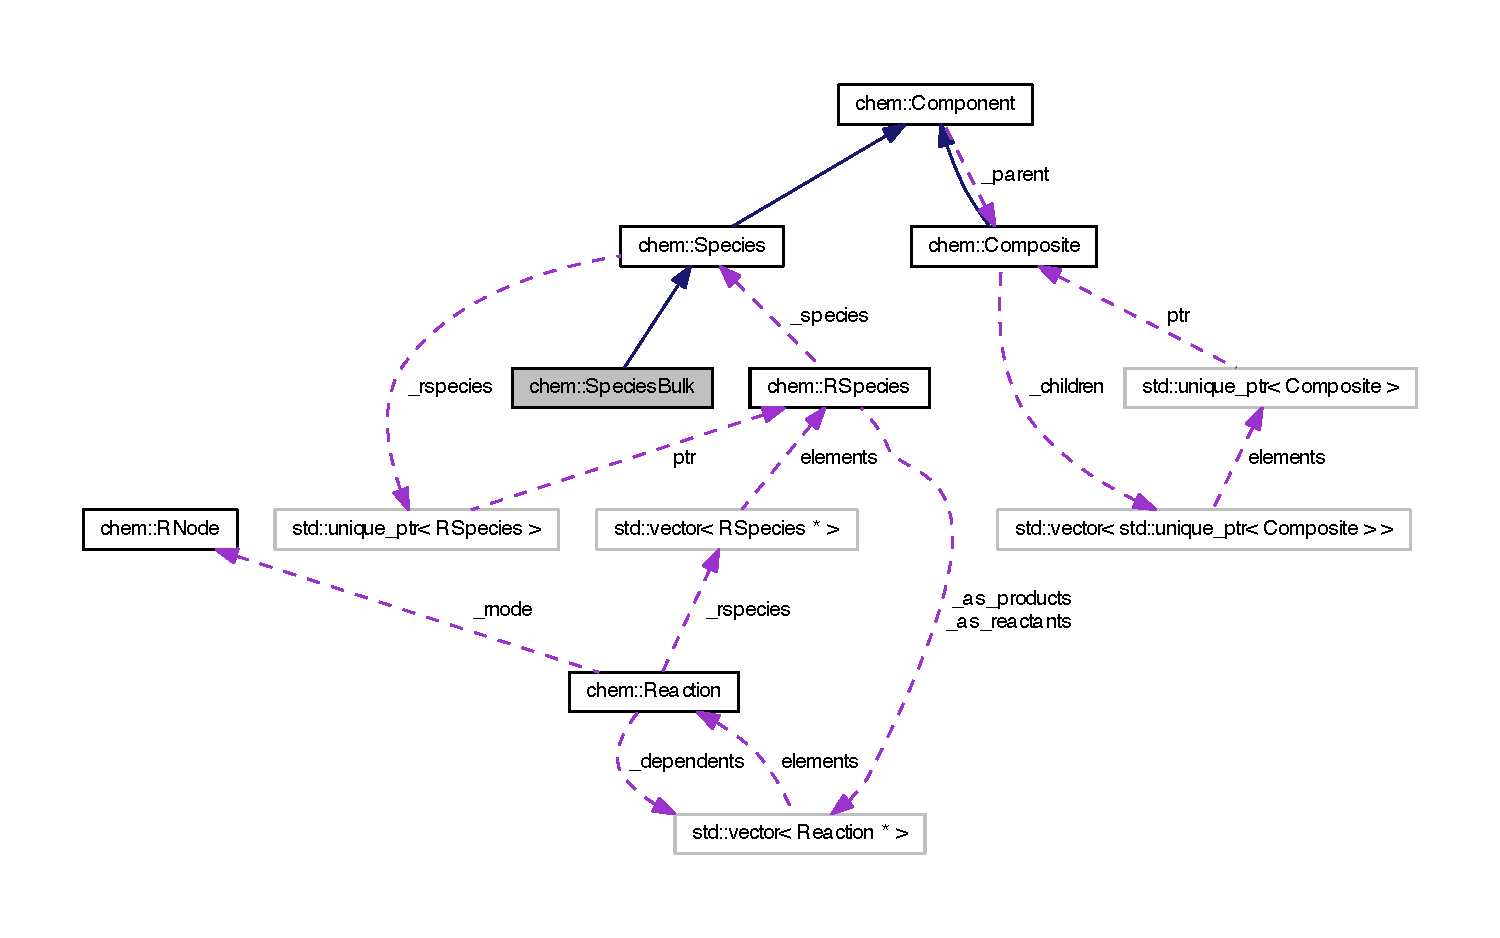
\includegraphics[width=350pt]{classchem_1_1SpeciesBulk__coll__graph}
\end{center}
\end{figure}
\subsection*{Public Member Functions}
\begin{DoxyCompactItemize}
\item 
\hyperlink{classchem_1_1SpeciesBulk_a1923eee58108af0529df6f9e7fdbc80e}{Species\-Bulk} ()
\begin{DoxyCompactList}\small\item\em Default constructor. \end{DoxyCompactList}\item 
\hyperlink{classchem_1_1SpeciesBulk_a8b4f80f5b0d6385250c936a24cca0d81}{Species\-Bulk} (const std\-::string \&name, \hyperlink{common_8h_a3503f321fd36304ee274141275cca586}{species\-\_\-copy\-\_\-t} n=0, \hyperlink{common_8h_a3503f321fd36304ee274141275cca586}{species\-\_\-copy\-\_\-t} ulim=\hyperlink{common_8h_adaf831a0b61083f29adf8fc6e8edab35}{max\-\_\-ulim})
\begin{DoxyCompactList}\small\item\em The main constructor. \end{DoxyCompactList}\item 
\hyperlink{classchem_1_1SpeciesBulk_a275b12de8e39aef164ed04c523181bfb}{Species\-Bulk} (const \hyperlink{classchem_1_1SpeciesBulk}{Species\-Bulk} \&rhs)
\begin{DoxyCompactList}\small\item\em Copy constructor. \end{DoxyCompactList}\item 
\hyperlink{classchem_1_1SpeciesBulk_ab53bee8acf46517803bea706ac7d9685}{Species\-Bulk} (\hyperlink{classchem_1_1SpeciesBulk}{Species\-Bulk} \&\&rhs) noexcept
\begin{DoxyCompactList}\small\item\em Move constructor. \end{DoxyCompactList}\item 
\hyperlink{classchem_1_1SpeciesBulk}{Species\-Bulk} \& \hyperlink{classchem_1_1SpeciesBulk_ad0e657ab81d9b37475dbc9235b2f48c4}{operator=} (const \hyperlink{classchem_1_1SpeciesBulk}{Species\-Bulk} \&rhs)
\begin{DoxyCompactList}\small\item\em Regular Assignment. \end{DoxyCompactList}\item 
\hyperlink{classchem_1_1SpeciesBulk}{Species\-Bulk} \& \hyperlink{classchem_1_1SpeciesBulk_a9ffd987e1f885746fcb6f6d5293692f3}{operator=} (\hyperlink{classchem_1_1SpeciesBulk}{Species\-Bulk} \&\&rhs)
\begin{DoxyCompactList}\small\item\em Move assignment. \end{DoxyCompactList}\item 
virtual \hyperlink{classchem_1_1SpeciesBulk}{Species\-Bulk} $\ast$ \hyperlink{classchem_1_1SpeciesBulk_a7bfdd13273d7328c2f7d275796e57873}{clone} ()
\item 
virtual std\-::string \hyperlink{classchem_1_1SpeciesBulk_a340d3f16e075352bf1cbab7918f5ca20}{get\-Full\-Name} () const 
\begin{DoxyCompactList}\small\item\em Return the full name of this \hyperlink{classchem_1_1Species}{Species} in a std\-::string format (e.\-g. \char`\"{}\-Arp2/3\{\-Bulk\}\char`\"{}. \end{DoxyCompactList}\item 
\hyperlink{classchem_1_1SpeciesBulk_ae9f7976efc0117e213b1a616e1216d5d}{$\sim$\-Species\-Bulk} () noexcept
\begin{DoxyCompactList}\small\item\em Default destructor. \end{DoxyCompactList}\item 
\hyperlink{classchem_1_1Composite}{Composite} $\ast$ \hyperlink{classchem_1_1Species_acdc83314b339310022d56e024f124a34}{get\-Parent} ()
\item 
void \hyperlink{classchem_1_1Species_a50e1e828d0b8a03efc9354e2c00174f5}{set\-Parent} (\hyperlink{classchem_1_1Composite}{Composite} $\ast$other)
\item 
bool \hyperlink{classchem_1_1Species_a6ddddc5be2b0e4427486f80a891879b3}{has\-Parent} () const 
\item 
\hyperlink{classchem_1_1Composite}{Composite} $\ast$ \hyperlink{classchem_1_1Species_aa5931e2aae4856c1b438691c23ada5aa}{get\-Root} ()
\item 
\hyperlink{classchem_1_1RSpecies}{R\-Species} \& \hyperlink{classchem_1_1Species_a1719a8155a69e9a62593d23d4bfc8514}{get\-R\-Species} ()
\begin{DoxyCompactList}\small\item\em Return a reference to \hyperlink{classchem_1_1RSpecies}{R\-Species}. \end{DoxyCompactList}\item 
const \hyperlink{classchem_1_1RSpecies}{R\-Species} \& \hyperlink{classchem_1_1Species_a438dae186317809effdd040ed38c568b}{get\-R\-Species} () const 
\begin{DoxyCompactList}\small\item\em Return a constant reference to \hyperlink{classchem_1_1RSpecies}{R\-Species}. \end{DoxyCompactList}\item 
void \hyperlink{classchem_1_1Species_af10a33a212fdb986fb93613e9c219f7a}{set\-N} (\hyperlink{common_8h_a3503f321fd36304ee274141275cca586}{species\-\_\-copy\-\_\-t} n)
\begin{DoxyCompactList}\small\item\em Sets the copy number for this \hyperlink{classchem_1_1Species}{Species}. \end{DoxyCompactList}\item 
\hyperlink{common_8h_a3503f321fd36304ee274141275cca586}{species\-\_\-copy\-\_\-t} \hyperlink{classchem_1_1Species_af7c9f51060b84169b428a7796dad6dca}{get\-N} () const 
\begin{DoxyCompactList}\small\item\em Return the current copy number of this \hyperlink{classchem_1_1Species}{Species}. \end{DoxyCompactList}\item 
std\-::string \hyperlink{classchem_1_1Species_aa32c8f7fb344c68539a927c6a7f916c7}{get\-Name} () const 
\begin{DoxyCompactList}\small\item\em Return this \hyperlink{classchem_1_1Species}{Species}' name. \end{DoxyCompactList}\item 
int \hyperlink{classchem_1_1Species_a330ef4514a8979a6ea0e6f71ed5cb820}{get\-Molecule} () const 
\begin{DoxyCompactList}\small\item\em Return the molecule index associated with this \hyperlink{classchem_1_1Species}{Species}' (as int) \end{DoxyCompactList}\item 
virtual size\-\_\-t \hyperlink{classchem_1_1Species_a5e8aedfe4c4b5e08fb0ee672c3d80ace}{count\-Species} () const 
\end{DoxyCompactItemize}
\subsection*{Friends}
\begin{DoxyCompactItemize}
\item 
bool \hyperlink{classchem_1_1Species_a22987c5719b74c50465256ea5b9d80bf}{operator==} (const \hyperlink{classchem_1_1Species}{Species} \&a, const \hyperlink{classchem_1_1Species}{Species} \&b)
\begin{DoxyCompactList}\small\item\em Returns true if two \hyperlink{classchem_1_1Species}{Species} objects are equal. \end{DoxyCompactList}\item 
bool \hyperlink{classchem_1_1Species_aff630d716711fbbab3bc7f598230316b}{operator!=} (const \hyperlink{classchem_1_1Species}{Species} \&a, const \hyperlink{classchem_1_1Species}{Species} \&b)
\begin{DoxyCompactList}\small\item\em Return true if two \hyperlink{classchem_1_1Species}{Species} are not equal. \end{DoxyCompactList}\end{DoxyCompactItemize}


\subsection{Detailed Description}
\hyperlink{classchem_1_1SpeciesBulk}{Species\-Bulk} should be used for \hyperlink{classchem_1_1Species}{Species} without spatial information (i.\-e. well-\/mixed in the container) 

Definition at line 289 of file Species.\-h.



\subsection{Constructor \& Destructor Documentation}
\hypertarget{classchem_1_1SpeciesBulk_a1923eee58108af0529df6f9e7fdbc80e}{\index{chem\-::\-Species\-Bulk@{chem\-::\-Species\-Bulk}!Species\-Bulk@{Species\-Bulk}}
\index{Species\-Bulk@{Species\-Bulk}!chem::SpeciesBulk@{chem\-::\-Species\-Bulk}}
\subsubsection[{Species\-Bulk}]{\setlength{\rightskip}{0pt plus 5cm}{\bf chem\-::\-Species\-Bulk\-::\-Species\-Bulk} (
\begin{DoxyParamCaption}
{}
\end{DoxyParamCaption}
)\hspace{0.3cm}{\ttfamily  \mbox{[}inline\mbox{]}}}}\label{classchem_1_1SpeciesBulk_a1923eee58108af0529df6f9e7fdbc80e}


Default constructor. 



Definition at line 292 of file Species.\-h.



Referenced by clone().

\hypertarget{classchem_1_1SpeciesBulk_a8b4f80f5b0d6385250c936a24cca0d81}{\index{chem\-::\-Species\-Bulk@{chem\-::\-Species\-Bulk}!Species\-Bulk@{Species\-Bulk}}
\index{Species\-Bulk@{Species\-Bulk}!chem::SpeciesBulk@{chem\-::\-Species\-Bulk}}
\subsubsection[{Species\-Bulk}]{\setlength{\rightskip}{0pt plus 5cm}{\bf chem\-::\-Species\-Bulk\-::\-Species\-Bulk} (
\begin{DoxyParamCaption}
\item[{const std\-::string \&}]{name, }
\item[{{\bf species\-\_\-copy\-\_\-t}}]{n = {\ttfamily 0}, }
\item[{{\bf species\-\_\-copy\-\_\-t}}]{ulim = {\ttfamily {\bf max\-\_\-ulim}}}
\end{DoxyParamCaption}
)\hspace{0.3cm}{\ttfamily  \mbox{[}inline\mbox{]}}}}\label{classchem_1_1SpeciesBulk_a8b4f80f5b0d6385250c936a24cca0d81}


The main constructor. 


\begin{DoxyParams}{Parameters}
{\em name} & -\/ Example, \char`\"{}\-G-\/\-Actin\char`\"{} or \char`\"{}\-Arp2/3\char`\"{} \\
\hline
{\em n} & -\/ copy number \\
\hline
\end{DoxyParams}


Definition at line 297 of file Species.\-h.

\hypertarget{classchem_1_1SpeciesBulk_a275b12de8e39aef164ed04c523181bfb}{\index{chem\-::\-Species\-Bulk@{chem\-::\-Species\-Bulk}!Species\-Bulk@{Species\-Bulk}}
\index{Species\-Bulk@{Species\-Bulk}!chem::SpeciesBulk@{chem\-::\-Species\-Bulk}}
\subsubsection[{Species\-Bulk}]{\setlength{\rightskip}{0pt plus 5cm}{\bf chem\-::\-Species\-Bulk\-::\-Species\-Bulk} (
\begin{DoxyParamCaption}
\item[{const {\bf Species\-Bulk} \&}]{rhs}
\end{DoxyParamCaption}
)\hspace{0.3cm}{\ttfamily  \mbox{[}inline\mbox{]}}}}\label{classchem_1_1SpeciesBulk_a275b12de8e39aef164ed04c523181bfb}


Copy constructor. 



Definition at line 300 of file Species.\-h.

\hypertarget{classchem_1_1SpeciesBulk_ab53bee8acf46517803bea706ac7d9685}{\index{chem\-::\-Species\-Bulk@{chem\-::\-Species\-Bulk}!Species\-Bulk@{Species\-Bulk}}
\index{Species\-Bulk@{Species\-Bulk}!chem::SpeciesBulk@{chem\-::\-Species\-Bulk}}
\subsubsection[{Species\-Bulk}]{\setlength{\rightskip}{0pt plus 5cm}{\bf chem\-::\-Species\-Bulk\-::\-Species\-Bulk} (
\begin{DoxyParamCaption}
\item[{{\bf Species\-Bulk} \&\&}]{rhs}
\end{DoxyParamCaption}
)\hspace{0.3cm}{\ttfamily  \mbox{[}inline\mbox{]}}}}\label{classchem_1_1SpeciesBulk_ab53bee8acf46517803bea706ac7d9685}


Move constructor. 



Definition at line 303 of file Species.\-h.

\hypertarget{classchem_1_1SpeciesBulk_ae9f7976efc0117e213b1a616e1216d5d}{\index{chem\-::\-Species\-Bulk@{chem\-::\-Species\-Bulk}!$\sim$\-Species\-Bulk@{$\sim$\-Species\-Bulk}}
\index{$\sim$\-Species\-Bulk@{$\sim$\-Species\-Bulk}!chem::SpeciesBulk@{chem\-::\-Species\-Bulk}}
\subsubsection[{$\sim$\-Species\-Bulk}]{\setlength{\rightskip}{0pt plus 5cm}{\bf chem\-::\-Species\-Bulk\-::$\sim$\-Species\-Bulk} (
\begin{DoxyParamCaption}
{}
\end{DoxyParamCaption}
)\hspace{0.3cm}{\ttfamily  \mbox{[}inline\mbox{]}}}}\label{classchem_1_1SpeciesBulk_ae9f7976efc0117e213b1a616e1216d5d}


Default destructor. 



Definition at line 327 of file Species.\-h.



\subsection{Member Function Documentation}
\hypertarget{classchem_1_1SpeciesBulk_a7bfdd13273d7328c2f7d275796e57873}{\index{chem\-::\-Species\-Bulk@{chem\-::\-Species\-Bulk}!clone@{clone}}
\index{clone@{clone}!chem::SpeciesBulk@{chem\-::\-Species\-Bulk}}
\subsubsection[{clone}]{\setlength{\rightskip}{0pt plus 5cm}virtual {\bf Species\-Bulk}$\ast$ {\bf chem\-::\-Species\-Bulk\-::clone} (
\begin{DoxyParamCaption}
{}
\end{DoxyParamCaption}
)\hspace{0.3cm}{\ttfamily  \mbox{[}inline, virtual\mbox{]}}}}\label{classchem_1_1SpeciesBulk_a7bfdd13273d7328c2f7d275796e57873}


Reimplemented from \hyperlink{classchem_1_1Species_acf0054a3704627698ba91293e8d0d370}{chem\-::\-Species}.



Definition at line 319 of file Species.\-h.



References Species\-Bulk().

\hypertarget{classchem_1_1Species_a5e8aedfe4c4b5e08fb0ee672c3d80ace}{\index{chem\-::\-Species\-Bulk@{chem\-::\-Species\-Bulk}!count\-Species@{count\-Species}}
\index{count\-Species@{count\-Species}!chem::SpeciesBulk@{chem\-::\-Species\-Bulk}}
\subsubsection[{count\-Species}]{\setlength{\rightskip}{0pt plus 5cm}virtual size\-\_\-t {\bf chem\-::\-Species\-::count\-Species} (
\begin{DoxyParamCaption}
{}
\end{DoxyParamCaption}
) const\hspace{0.3cm}{\ttfamily  \mbox{[}inline, virtual, inherited\mbox{]}}}}\label{classchem_1_1Species_a5e8aedfe4c4b5e08fb0ee672c3d80ace}


Definition at line 285 of file Species.\-h.

\hypertarget{classchem_1_1SpeciesBulk_a340d3f16e075352bf1cbab7918f5ca20}{\index{chem\-::\-Species\-Bulk@{chem\-::\-Species\-Bulk}!get\-Full\-Name@{get\-Full\-Name}}
\index{get\-Full\-Name@{get\-Full\-Name}!chem::SpeciesBulk@{chem\-::\-Species\-Bulk}}
\subsubsection[{get\-Full\-Name}]{\setlength{\rightskip}{0pt plus 5cm}virtual std\-::string {\bf chem\-::\-Species\-Bulk\-::get\-Full\-Name} (
\begin{DoxyParamCaption}
{}
\end{DoxyParamCaption}
) const\hspace{0.3cm}{\ttfamily  \mbox{[}inline, virtual\mbox{]}}}}\label{classchem_1_1SpeciesBulk_a340d3f16e075352bf1cbab7918f5ca20}


Return the full name of this \hyperlink{classchem_1_1Species}{Species} in a std\-::string format (e.\-g. \char`\"{}\-Arp2/3\{\-Bulk\}\char`\"{}. 



Reimplemented from \hyperlink{classchem_1_1Species_a7ac7196a7146f63e297d0995c6081f4b}{chem\-::\-Species}.



Definition at line 324 of file Species.\-h.



References chem\-::\-Species\-::get\-Name().

\hypertarget{classchem_1_1Species_a330ef4514a8979a6ea0e6f71ed5cb820}{\index{chem\-::\-Species\-Bulk@{chem\-::\-Species\-Bulk}!get\-Molecule@{get\-Molecule}}
\index{get\-Molecule@{get\-Molecule}!chem::SpeciesBulk@{chem\-::\-Species\-Bulk}}
\subsubsection[{get\-Molecule}]{\setlength{\rightskip}{0pt plus 5cm}int {\bf chem\-::\-Species\-::get\-Molecule} (
\begin{DoxyParamCaption}
{}
\end{DoxyParamCaption}
) const\hspace{0.3cm}{\ttfamily  \mbox{[}inline, inherited\mbox{]}}}}\label{classchem_1_1Species_a330ef4514a8979a6ea0e6f71ed5cb820}


Return the molecule index associated with this \hyperlink{classchem_1_1Species}{Species}' (as int) 



Definition at line 231 of file Species.\-h.



References chem\-::\-Species\-::\-\_\-molecule.



Referenced by chem\-::\-Compartment\-::add\-Species(), chem\-::\-Compartment\-::add\-Species\-Unique(), and chem\-::\-Compartment\-::set\-Diffusion\-Rate().

\hypertarget{classchem_1_1Species_af7c9f51060b84169b428a7796dad6dca}{\index{chem\-::\-Species\-Bulk@{chem\-::\-Species\-Bulk}!get\-N@{get\-N}}
\index{get\-N@{get\-N}!chem::SpeciesBulk@{chem\-::\-Species\-Bulk}}
\subsubsection[{get\-N}]{\setlength{\rightskip}{0pt plus 5cm}{\bf species\-\_\-copy\-\_\-t} {\bf chem\-::\-Species\-::get\-N} (
\begin{DoxyParamCaption}
{}
\end{DoxyParamCaption}
) const\hspace{0.3cm}{\ttfamily  \mbox{[}inline, inherited\mbox{]}}}}\label{classchem_1_1Species_af7c9f51060b84169b428a7796dad6dca}


Return the current copy number of this \hyperlink{classchem_1_1Species}{Species}. 



Definition at line 220 of file Species.\-h.



References chem\-::\-Species\-::\-\_\-rspecies, and chem\-::\-R\-Species\-::get\-N().



Referenced by operator$<$$<$(), chem\-::\-Species\-::operator=(), and chem\-::\-Species\-::\-Species().

\hypertarget{classchem_1_1Species_aa32c8f7fb344c68539a927c6a7f916c7}{\index{chem\-::\-Species\-Bulk@{chem\-::\-Species\-Bulk}!get\-Name@{get\-Name}}
\index{get\-Name@{get\-Name}!chem::SpeciesBulk@{chem\-::\-Species\-Bulk}}
\subsubsection[{get\-Name}]{\setlength{\rightskip}{0pt plus 5cm}std\-::string {\bf chem\-::\-Species\-::get\-Name} (
\begin{DoxyParamCaption}
{}
\end{DoxyParamCaption}
) const\hspace{0.3cm}{\ttfamily  \mbox{[}inline, inherited\mbox{]}}}}\label{classchem_1_1Species_aa32c8f7fb344c68539a927c6a7f916c7}


Return this \hyperlink{classchem_1_1Species}{Species}' name. 



Definition at line 228 of file Species.\-h.



References chem\-::\-Species\-::\-\_\-molecule, chem\-::\-Species\-Names\-D\-B\-::\-Instance(), and chem\-::\-Species\-Names\-D\-B\-::int\-To\-String().



Referenced by chem\-::\-Species\-::get\-Full\-Name(), get\-Full\-Name(), and chem\-::\-Species\-Diffusing\-::get\-Full\-Name().

\hypertarget{classchem_1_1Species_acdc83314b339310022d56e024f124a34}{\index{chem\-::\-Species\-Bulk@{chem\-::\-Species\-Bulk}!get\-Parent@{get\-Parent}}
\index{get\-Parent@{get\-Parent}!chem::SpeciesBulk@{chem\-::\-Species\-Bulk}}
\subsubsection[{get\-Parent}]{\setlength{\rightskip}{0pt plus 5cm}{\bf Composite}$\ast$ {\bf chem\-::\-Species\-::get\-Parent} (
\begin{DoxyParamCaption}
{}
\end{DoxyParamCaption}
)\hspace{0.3cm}{\ttfamily  \mbox{[}inline, inherited\mbox{]}}}}\label{classchem_1_1Species_acdc83314b339310022d56e024f124a34}


Definition at line 199 of file Species.\-h.



References chem\-::\-Species\-::\-\_\-parent.



Referenced by chem\-::\-Species\-::get\-Root().

\hypertarget{classchem_1_1Species_aa5931e2aae4856c1b438691c23ada5aa}{\index{chem\-::\-Species\-Bulk@{chem\-::\-Species\-Bulk}!get\-Root@{get\-Root}}
\index{get\-Root@{get\-Root}!chem::SpeciesBulk@{chem\-::\-Species\-Bulk}}
\subsubsection[{get\-Root}]{\setlength{\rightskip}{0pt plus 5cm}{\bf Composite} $\ast$ {\bf chem\-::\-Species\-::get\-Root} (
\begin{DoxyParamCaption}
{}
\end{DoxyParamCaption}
)\hspace{0.3cm}{\ttfamily  \mbox{[}inherited\mbox{]}}}}\label{classchem_1_1Species_aa5931e2aae4856c1b438691c23ada5aa}


Definition at line 35 of file Species.\-cpp.



References chem\-::\-Species\-::get\-Parent(), chem\-::\-Component\-::get\-Root(), and chem\-::\-Species\-::has\-Parent().

\hypertarget{classchem_1_1Species_a1719a8155a69e9a62593d23d4bfc8514}{\index{chem\-::\-Species\-Bulk@{chem\-::\-Species\-Bulk}!get\-R\-Species@{get\-R\-Species}}
\index{get\-R\-Species@{get\-R\-Species}!chem::SpeciesBulk@{chem\-::\-Species\-Bulk}}
\subsubsection[{get\-R\-Species}]{\setlength{\rightskip}{0pt plus 5cm}{\bf R\-Species}\& {\bf chem\-::\-Species\-::get\-R\-Species} (
\begin{DoxyParamCaption}
{}
\end{DoxyParamCaption}
)\hspace{0.3cm}{\ttfamily  \mbox{[}inline, inherited\mbox{]}}}}\label{classchem_1_1Species_a1719a8155a69e9a62593d23d4bfc8514}


Return a reference to \hyperlink{classchem_1_1RSpecies}{R\-Species}. 

Notice that value copying won't be allowed because \hyperlink{classchem_1_1RSpecies}{R\-Species} is not copyable. 

Definition at line 209 of file Species.\-h.



References chem\-::\-Species\-::\-\_\-rspecies.



Referenced by chem\-::\-Chem\-Signal\-::connect(), and main().

\hypertarget{classchem_1_1Species_a438dae186317809effdd040ed38c568b}{\index{chem\-::\-Species\-Bulk@{chem\-::\-Species\-Bulk}!get\-R\-Species@{get\-R\-Species}}
\index{get\-R\-Species@{get\-R\-Species}!chem::SpeciesBulk@{chem\-::\-Species\-Bulk}}
\subsubsection[{get\-R\-Species}]{\setlength{\rightskip}{0pt plus 5cm}const {\bf R\-Species}\& {\bf chem\-::\-Species\-::get\-R\-Species} (
\begin{DoxyParamCaption}
{}
\end{DoxyParamCaption}
) const\hspace{0.3cm}{\ttfamily  \mbox{[}inline, inherited\mbox{]}}}}\label{classchem_1_1Species_a438dae186317809effdd040ed38c568b}


Return a constant reference to \hyperlink{classchem_1_1RSpecies}{R\-Species}. 



Definition at line 212 of file Species.\-h.



References chem\-::\-Species\-::\-\_\-rspecies.

\hypertarget{classchem_1_1Species_a6ddddc5be2b0e4427486f80a891879b3}{\index{chem\-::\-Species\-Bulk@{chem\-::\-Species\-Bulk}!has\-Parent@{has\-Parent}}
\index{has\-Parent@{has\-Parent}!chem::SpeciesBulk@{chem\-::\-Species\-Bulk}}
\subsubsection[{has\-Parent}]{\setlength{\rightskip}{0pt plus 5cm}bool {\bf chem\-::\-Species\-::has\-Parent} (
\begin{DoxyParamCaption}
{}
\end{DoxyParamCaption}
) const\hspace{0.3cm}{\ttfamily  \mbox{[}inline, inherited\mbox{]}}}}\label{classchem_1_1Species_a6ddddc5be2b0e4427486f80a891879b3}


Definition at line 203 of file Species.\-h.



References chem\-::\-Species\-::\-\_\-parent.



Referenced by chem\-::\-Species\-::get\-Root().

\hypertarget{classchem_1_1SpeciesBulk_ad0e657ab81d9b37475dbc9235b2f48c4}{\index{chem\-::\-Species\-Bulk@{chem\-::\-Species\-Bulk}!operator=@{operator=}}
\index{operator=@{operator=}!chem::SpeciesBulk@{chem\-::\-Species\-Bulk}}
\subsubsection[{operator=}]{\setlength{\rightskip}{0pt plus 5cm}{\bf Species\-Bulk}\& chem\-::\-Species\-Bulk\-::operator= (
\begin{DoxyParamCaption}
\item[{const {\bf Species\-Bulk} \&}]{rhs}
\end{DoxyParamCaption}
)\hspace{0.3cm}{\ttfamily  \mbox{[}inline\mbox{]}}}}\label{classchem_1_1SpeciesBulk_ad0e657ab81d9b37475dbc9235b2f48c4}


Regular Assignment. 



Definition at line 307 of file Species.\-h.



Referenced by operator=().

\hypertarget{classchem_1_1SpeciesBulk_a9ffd987e1f885746fcb6f6d5293692f3}{\index{chem\-::\-Species\-Bulk@{chem\-::\-Species\-Bulk}!operator=@{operator=}}
\index{operator=@{operator=}!chem::SpeciesBulk@{chem\-::\-Species\-Bulk}}
\subsubsection[{operator=}]{\setlength{\rightskip}{0pt plus 5cm}{\bf Species\-Bulk}\& chem\-::\-Species\-Bulk\-::operator= (
\begin{DoxyParamCaption}
\item[{{\bf Species\-Bulk} \&\&}]{rhs}
\end{DoxyParamCaption}
)\hspace{0.3cm}{\ttfamily  \mbox{[}inline\mbox{]}}}}\label{classchem_1_1SpeciesBulk_a9ffd987e1f885746fcb6f6d5293692f3}


Move assignment. 



Definition at line 313 of file Species.\-h.



References operator=().

\hypertarget{classchem_1_1Species_af10a33a212fdb986fb93613e9c219f7a}{\index{chem\-::\-Species\-Bulk@{chem\-::\-Species\-Bulk}!set\-N@{set\-N}}
\index{set\-N@{set\-N}!chem::SpeciesBulk@{chem\-::\-Species\-Bulk}}
\subsubsection[{set\-N}]{\setlength{\rightskip}{0pt plus 5cm}void {\bf chem\-::\-Species\-::set\-N} (
\begin{DoxyParamCaption}
\item[{{\bf species\-\_\-copy\-\_\-t}}]{n}
\end{DoxyParamCaption}
)\hspace{0.3cm}{\ttfamily  \mbox{[}inline, inherited\mbox{]}}}}\label{classchem_1_1Species_af10a33a212fdb986fb93613e9c219f7a}


Sets the copy number for this \hyperlink{classchem_1_1Species}{Species}. 


\begin{DoxyParams}{Parameters}
{\em n} & should be a non-\/negative number, but no checking is done in run time \\
\hline
\end{DoxyParams}
\begin{DoxyNote}{Note}
The operation does not emit any signals about the copy number change. 
\end{DoxyNote}


Definition at line 217 of file Species.\-h.



References chem\-::\-Species\-::\-\_\-rspecies, and chem\-::\-R\-Species\-::set\-N().



Referenced by main().

\hypertarget{classchem_1_1Species_a50e1e828d0b8a03efc9354e2c00174f5}{\index{chem\-::\-Species\-Bulk@{chem\-::\-Species\-Bulk}!set\-Parent@{set\-Parent}}
\index{set\-Parent@{set\-Parent}!chem::SpeciesBulk@{chem\-::\-Species\-Bulk}}
\subsubsection[{set\-Parent}]{\setlength{\rightskip}{0pt plus 5cm}void {\bf chem\-::\-Species\-::set\-Parent} (
\begin{DoxyParamCaption}
\item[{{\bf Composite} $\ast$}]{other}
\end{DoxyParamCaption}
)\hspace{0.3cm}{\ttfamily  \mbox{[}inline, inherited\mbox{]}}}}\label{classchem_1_1Species_a50e1e828d0b8a03efc9354e2c00174f5}


Definition at line 201 of file Species.\-h.



References chem\-::\-Species\-::\-\_\-parent.



Referenced by chem\-::\-Compartment\-::add\-Species(), and chem\-::\-Compartment\-::add\-Species\-Unique().



\subsection{Friends And Related Function Documentation}
\hypertarget{classchem_1_1Species_aff630d716711fbbab3bc7f598230316b}{\index{chem\-::\-Species\-Bulk@{chem\-::\-Species\-Bulk}!operator!=@{operator!=}}
\index{operator!=@{operator!=}!chem::SpeciesBulk@{chem\-::\-Species\-Bulk}}
\subsubsection[{operator!=}]{\setlength{\rightskip}{0pt plus 5cm}bool operator!= (
\begin{DoxyParamCaption}
\item[{const {\bf Species} \&}]{a, }
\item[{const {\bf Species} \&}]{b}
\end{DoxyParamCaption}
)\hspace{0.3cm}{\ttfamily  \mbox{[}friend, inherited\mbox{]}}}}\label{classchem_1_1Species_aff630d716711fbbab3bc7f598230316b}


Return true if two \hyperlink{classchem_1_1Species}{Species} are not equal. 

\begin{DoxySeeAlso}{See also}
\hyperlink{classchem_1_1Species_a22987c5719b74c50465256ea5b9d80bf}{operator ==(const Species\& a, const Species\& b)} above 
\end{DoxySeeAlso}


Definition at line 266 of file Species.\-h.

\hypertarget{classchem_1_1Species_a22987c5719b74c50465256ea5b9d80bf}{\index{chem\-::\-Species\-Bulk@{chem\-::\-Species\-Bulk}!operator==@{operator==}}
\index{operator==@{operator==}!chem::SpeciesBulk@{chem\-::\-Species\-Bulk}}
\subsubsection[{operator==}]{\setlength{\rightskip}{0pt plus 5cm}bool operator== (
\begin{DoxyParamCaption}
\item[{const {\bf Species} \&}]{a, }
\item[{const {\bf Species} \&}]{b}
\end{DoxyParamCaption}
)\hspace{0.3cm}{\ttfamily  \mbox{[}friend, inherited\mbox{]}}}}\label{classchem_1_1Species_a22987c5719b74c50465256ea5b9d80bf}


Returns true if two \hyperlink{classchem_1_1Species}{Species} objects are equal. 

This function would accept derived class of \hyperlink{classchem_1_1Species}{Species}, such as \hyperlink{classchem_1_1SpeciesBulk}{Species\-Bulk} Two \hyperlink{classchem_1_1Species}{Species} are equal if their S\-Type(s) are equal (i.\-e. are of the same class), their names are equal. 

Definition at line 257 of file Species.\-h.



The documentation for this class was generated from the following file\-:\begin{DoxyCompactItemize}
\item 
Cyto\-Sim/\hyperlink{Species_8h}{Species.\-h}\end{DoxyCompactItemize}

\input{classchem_1_1SpeciesContainerIFace}
\input{classchem_1_1SpeciesContainerVector}
\hypertarget{classchem_1_1SpeciesDiffusing}{\section{chem\-:\-:Species\-Diffusing Class Reference}
\label{classchem_1_1SpeciesDiffusing}\index{chem\-::\-Species\-Diffusing@{chem\-::\-Species\-Diffusing}}
}


\hyperlink{classchem_1_1SpeciesDiffusing}{Species\-Diffusing} should be used for \hyperlink{classchem_1_1Species}{Species} which can move spatially from one compartment to the neighboring one (i.\-e. they are the stochastic analogue of determenistic reaction-\/diffusion processes)  




{\ttfamily \#include $<$Species.\-h$>$}



Inheritance diagram for chem\-:\-:Species\-Diffusing\-:
\nopagebreak
\begin{figure}[H]
\begin{center}
\leavevmode
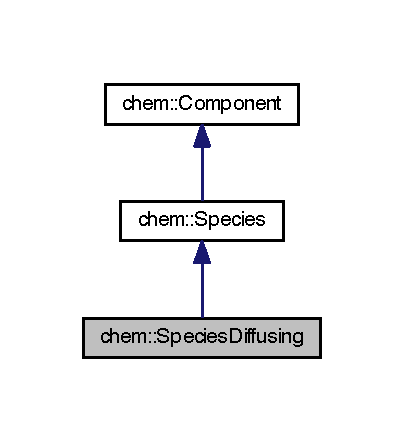
\includegraphics[width=194pt]{classchem_1_1SpeciesDiffusing__inherit__graph}
\end{center}
\end{figure}


Collaboration diagram for chem\-:\-:Species\-Diffusing\-:
\nopagebreak
\begin{figure}[H]
\begin{center}
\leavevmode
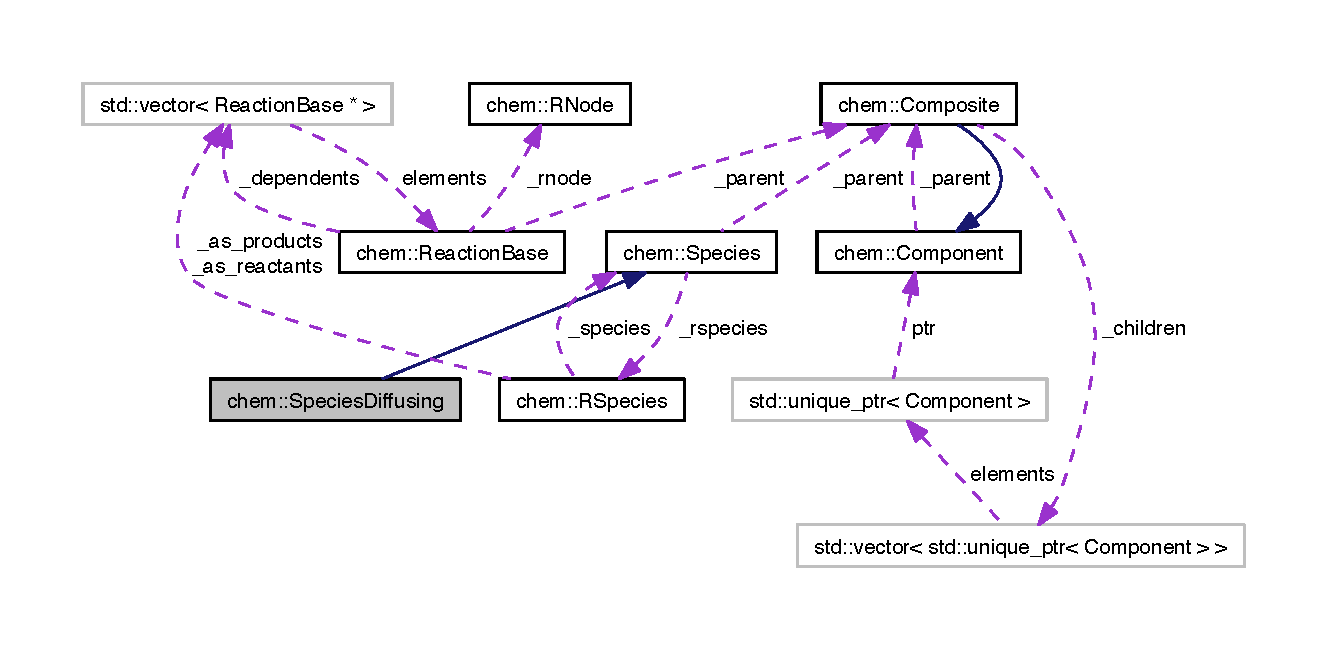
\includegraphics[width=350pt]{classchem_1_1SpeciesDiffusing__coll__graph}
\end{center}
\end{figure}
\subsection*{Public Member Functions}
\begin{DoxyCompactItemize}
\item 
\hyperlink{classchem_1_1SpeciesDiffusing_a2f590ce263086be62eb7998afd4abda4}{Species\-Diffusing} ()
\begin{DoxyCompactList}\small\item\em Default constructor. \end{DoxyCompactList}\item 
\hyperlink{classchem_1_1SpeciesDiffusing_aa0183d61ee28bcc845674d3b649bf100}{Species\-Diffusing} (const std\-::string \&name, \hyperlink{common_8h_a3503f321fd36304ee274141275cca586}{species\-\_\-copy\-\_\-t} n=0, \hyperlink{common_8h_a3503f321fd36304ee274141275cca586}{species\-\_\-copy\-\_\-t} ulim=\hyperlink{common_8h_adaf831a0b61083f29adf8fc6e8edab35}{max\-\_\-ulim})
\begin{DoxyCompactList}\small\item\em The main constructor. \end{DoxyCompactList}\item 
\hyperlink{classchem_1_1SpeciesDiffusing_ae5a9f9e77809772866d2bbfb440ae817}{Species\-Diffusing} (const \hyperlink{classchem_1_1SpeciesDiffusing}{Species\-Diffusing} \&rhs)
\begin{DoxyCompactList}\small\item\em Copy constructor. \end{DoxyCompactList}\item 
\hyperlink{classchem_1_1SpeciesDiffusing_a560f9bc8c0d7da4a91a969e78917afa4}{Species\-Diffusing} (\hyperlink{classchem_1_1SpeciesDiffusing}{Species\-Diffusing} \&\&rhs) noexcept
\begin{DoxyCompactList}\small\item\em Move constructor. \end{DoxyCompactList}\item 
\hyperlink{classchem_1_1SpeciesDiffusing}{Species\-Diffusing} \& \hyperlink{classchem_1_1SpeciesDiffusing_a88592474fe2dd281951e15c6b8ddf201}{operator=} (const \hyperlink{classchem_1_1SpeciesDiffusing}{Species\-Diffusing} \&rhs)
\begin{DoxyCompactList}\small\item\em Regular Assignment. \end{DoxyCompactList}\item 
\hyperlink{classchem_1_1SpeciesDiffusing}{Species\-Diffusing} \& \hyperlink{classchem_1_1SpeciesDiffusing_add1696a25d2174de8078ef509b313890}{operator=} (\hyperlink{classchem_1_1SpeciesDiffusing}{Species\-Diffusing} \&\&rhs)
\begin{DoxyCompactList}\small\item\em Move assignment. \end{DoxyCompactList}\item 
virtual \hyperlink{classchem_1_1SpeciesDiffusing}{Species\-Diffusing} $\ast$ \hyperlink{classchem_1_1SpeciesDiffusing_a69edbe33378230389a2fb99c4ca2b5ce}{clone} ()
\item 
virtual std\-::string \hyperlink{classchem_1_1SpeciesDiffusing_a03eba31a17a3713e8c45cc0952e922bb}{get\-Full\-Name} () const 
\begin{DoxyCompactList}\small\item\em Return the full name of this \hyperlink{classchem_1_1Species}{Species} in a std\-::string format (e.\-g. \char`\"{}\-Arp2/3\{\-Diffusing\}\char`\"{}. \end{DoxyCompactList}\item 
\hyperlink{classchem_1_1SpeciesDiffusing_a683ab39a97cef1b68be11c68b476a840}{$\sim$\-Species\-Diffusing} () noexcept
\begin{DoxyCompactList}\small\item\em Default destructor. \end{DoxyCompactList}\item 
\hyperlink{classchem_1_1Composite}{Composite} $\ast$ \hyperlink{classchem_1_1Species_acdc83314b339310022d56e024f124a34}{get\-Parent} ()
\item 
void \hyperlink{classchem_1_1Species_a50e1e828d0b8a03efc9354e2c00174f5}{set\-Parent} (\hyperlink{classchem_1_1Composite}{Composite} $\ast$other)
\item 
bool \hyperlink{classchem_1_1Species_a6ddddc5be2b0e4427486f80a891879b3}{has\-Parent} () const 
\item 
\hyperlink{classchem_1_1Composite}{Composite} $\ast$ \hyperlink{classchem_1_1Species_aa5931e2aae4856c1b438691c23ada5aa}{get\-Root} ()
\item 
\hyperlink{classchem_1_1RSpecies}{R\-Species} \& \hyperlink{classchem_1_1Species_a1719a8155a69e9a62593d23d4bfc8514}{get\-R\-Species} ()
\begin{DoxyCompactList}\small\item\em Return a reference to \hyperlink{classchem_1_1RSpecies}{R\-Species}. \end{DoxyCompactList}\item 
const \hyperlink{classchem_1_1RSpecies}{R\-Species} \& \hyperlink{classchem_1_1Species_a438dae186317809effdd040ed38c568b}{get\-R\-Species} () const 
\begin{DoxyCompactList}\small\item\em Return a constant reference to \hyperlink{classchem_1_1RSpecies}{R\-Species}. \end{DoxyCompactList}\item 
void \hyperlink{classchem_1_1Species_af10a33a212fdb986fb93613e9c219f7a}{set\-N} (\hyperlink{common_8h_a3503f321fd36304ee274141275cca586}{species\-\_\-copy\-\_\-t} n)
\begin{DoxyCompactList}\small\item\em Sets the copy number for this \hyperlink{classchem_1_1Species}{Species}. \end{DoxyCompactList}\item 
\hyperlink{common_8h_a3503f321fd36304ee274141275cca586}{species\-\_\-copy\-\_\-t} \hyperlink{classchem_1_1Species_af7c9f51060b84169b428a7796dad6dca}{get\-N} () const 
\begin{DoxyCompactList}\small\item\em Return the current copy number of this \hyperlink{classchem_1_1Species}{Species}. \end{DoxyCompactList}\item 
std\-::string \hyperlink{classchem_1_1Species_aa32c8f7fb344c68539a927c6a7f916c7}{get\-Name} () const 
\begin{DoxyCompactList}\small\item\em Return this \hyperlink{classchem_1_1Species}{Species}' name. \end{DoxyCompactList}\item 
int \hyperlink{classchem_1_1Species_a330ef4514a8979a6ea0e6f71ed5cb820}{get\-Molecule} () const 
\begin{DoxyCompactList}\small\item\em Return the molecule index associated with this \hyperlink{classchem_1_1Species}{Species}' (as int) \end{DoxyCompactList}\item 
virtual size\-\_\-t \hyperlink{classchem_1_1Species_a5e8aedfe4c4b5e08fb0ee672c3d80ace}{count\-Species} () const 
\end{DoxyCompactItemize}
\subsection*{Friends}
\begin{DoxyCompactItemize}
\item 
bool \hyperlink{classchem_1_1Species_a22987c5719b74c50465256ea5b9d80bf}{operator==} (const \hyperlink{classchem_1_1Species}{Species} \&a, const \hyperlink{classchem_1_1Species}{Species} \&b)
\begin{DoxyCompactList}\small\item\em Returns true if two \hyperlink{classchem_1_1Species}{Species} objects are equal. \end{DoxyCompactList}\item 
bool \hyperlink{classchem_1_1Species_aff630d716711fbbab3bc7f598230316b}{operator!=} (const \hyperlink{classchem_1_1Species}{Species} \&a, const \hyperlink{classchem_1_1Species}{Species} \&b)
\begin{DoxyCompactList}\small\item\em Return true if two \hyperlink{classchem_1_1Species}{Species} are not equal. \end{DoxyCompactList}\end{DoxyCompactItemize}


\subsection{Detailed Description}
\hyperlink{classchem_1_1SpeciesDiffusing}{Species\-Diffusing} should be used for \hyperlink{classchem_1_1Species}{Species} which can move spatially from one compartment to the neighboring one (i.\-e. they are the stochastic analogue of determenistic reaction-\/diffusion processes) 

Definition at line 331 of file Species.\-h.



\subsection{Constructor \& Destructor Documentation}
\hypertarget{classchem_1_1SpeciesDiffusing_a2f590ce263086be62eb7998afd4abda4}{\index{chem\-::\-Species\-Diffusing@{chem\-::\-Species\-Diffusing}!Species\-Diffusing@{Species\-Diffusing}}
\index{Species\-Diffusing@{Species\-Diffusing}!chem::SpeciesDiffusing@{chem\-::\-Species\-Diffusing}}
\subsubsection[{Species\-Diffusing}]{\setlength{\rightskip}{0pt plus 5cm}{\bf chem\-::\-Species\-Diffusing\-::\-Species\-Diffusing} (
\begin{DoxyParamCaption}
{}
\end{DoxyParamCaption}
)\hspace{0.3cm}{\ttfamily  \mbox{[}inline\mbox{]}}}}\label{classchem_1_1SpeciesDiffusing_a2f590ce263086be62eb7998afd4abda4}


Default constructor. 



Definition at line 334 of file Species.\-h.



Referenced by clone().

\hypertarget{classchem_1_1SpeciesDiffusing_aa0183d61ee28bcc845674d3b649bf100}{\index{chem\-::\-Species\-Diffusing@{chem\-::\-Species\-Diffusing}!Species\-Diffusing@{Species\-Diffusing}}
\index{Species\-Diffusing@{Species\-Diffusing}!chem::SpeciesDiffusing@{chem\-::\-Species\-Diffusing}}
\subsubsection[{Species\-Diffusing}]{\setlength{\rightskip}{0pt plus 5cm}{\bf chem\-::\-Species\-Diffusing\-::\-Species\-Diffusing} (
\begin{DoxyParamCaption}
\item[{const std\-::string \&}]{name, }
\item[{{\bf species\-\_\-copy\-\_\-t}}]{n = {\ttfamily 0}, }
\item[{{\bf species\-\_\-copy\-\_\-t}}]{ulim = {\ttfamily {\bf max\-\_\-ulim}}}
\end{DoxyParamCaption}
)\hspace{0.3cm}{\ttfamily  \mbox{[}inline\mbox{]}}}}\label{classchem_1_1SpeciesDiffusing_aa0183d61ee28bcc845674d3b649bf100}


The main constructor. 


\begin{DoxyParams}{Parameters}
{\em name} & -\/ Example, \char`\"{}\-G-\/\-Actin\char`\"{} or \char`\"{}\-Arp2/3\char`\"{} \\
\hline
{\em n} & -\/ copy number \\
\hline
\end{DoxyParams}


Definition at line 339 of file Species.\-h.

\hypertarget{classchem_1_1SpeciesDiffusing_ae5a9f9e77809772866d2bbfb440ae817}{\index{chem\-::\-Species\-Diffusing@{chem\-::\-Species\-Diffusing}!Species\-Diffusing@{Species\-Diffusing}}
\index{Species\-Diffusing@{Species\-Diffusing}!chem::SpeciesDiffusing@{chem\-::\-Species\-Diffusing}}
\subsubsection[{Species\-Diffusing}]{\setlength{\rightskip}{0pt plus 5cm}{\bf chem\-::\-Species\-Diffusing\-::\-Species\-Diffusing} (
\begin{DoxyParamCaption}
\item[{const {\bf Species\-Diffusing} \&}]{rhs}
\end{DoxyParamCaption}
)\hspace{0.3cm}{\ttfamily  \mbox{[}inline\mbox{]}}}}\label{classchem_1_1SpeciesDiffusing_ae5a9f9e77809772866d2bbfb440ae817}


Copy constructor. 



Definition at line 342 of file Species.\-h.

\hypertarget{classchem_1_1SpeciesDiffusing_a560f9bc8c0d7da4a91a969e78917afa4}{\index{chem\-::\-Species\-Diffusing@{chem\-::\-Species\-Diffusing}!Species\-Diffusing@{Species\-Diffusing}}
\index{Species\-Diffusing@{Species\-Diffusing}!chem::SpeciesDiffusing@{chem\-::\-Species\-Diffusing}}
\subsubsection[{Species\-Diffusing}]{\setlength{\rightskip}{0pt plus 5cm}{\bf chem\-::\-Species\-Diffusing\-::\-Species\-Diffusing} (
\begin{DoxyParamCaption}
\item[{{\bf Species\-Diffusing} \&\&}]{rhs}
\end{DoxyParamCaption}
)\hspace{0.3cm}{\ttfamily  \mbox{[}inline\mbox{]}}}}\label{classchem_1_1SpeciesDiffusing_a560f9bc8c0d7da4a91a969e78917afa4}


Move constructor. 



Definition at line 345 of file Species.\-h.

\hypertarget{classchem_1_1SpeciesDiffusing_a683ab39a97cef1b68be11c68b476a840}{\index{chem\-::\-Species\-Diffusing@{chem\-::\-Species\-Diffusing}!$\sim$\-Species\-Diffusing@{$\sim$\-Species\-Diffusing}}
\index{$\sim$\-Species\-Diffusing@{$\sim$\-Species\-Diffusing}!chem::SpeciesDiffusing@{chem\-::\-Species\-Diffusing}}
\subsubsection[{$\sim$\-Species\-Diffusing}]{\setlength{\rightskip}{0pt plus 5cm}{\bf chem\-::\-Species\-Diffusing\-::$\sim$\-Species\-Diffusing} (
\begin{DoxyParamCaption}
{}
\end{DoxyParamCaption}
)\hspace{0.3cm}{\ttfamily  \mbox{[}inline\mbox{]}}}}\label{classchem_1_1SpeciesDiffusing_a683ab39a97cef1b68be11c68b476a840}


Default destructor. 



Definition at line 369 of file Species.\-h.



\subsection{Member Function Documentation}
\hypertarget{classchem_1_1SpeciesDiffusing_a69edbe33378230389a2fb99c4ca2b5ce}{\index{chem\-::\-Species\-Diffusing@{chem\-::\-Species\-Diffusing}!clone@{clone}}
\index{clone@{clone}!chem::SpeciesDiffusing@{chem\-::\-Species\-Diffusing}}
\subsubsection[{clone}]{\setlength{\rightskip}{0pt plus 5cm}virtual {\bf Species\-Diffusing}$\ast$ {\bf chem\-::\-Species\-Diffusing\-::clone} (
\begin{DoxyParamCaption}
{}
\end{DoxyParamCaption}
)\hspace{0.3cm}{\ttfamily  \mbox{[}inline, virtual\mbox{]}}}}\label{classchem_1_1SpeciesDiffusing_a69edbe33378230389a2fb99c4ca2b5ce}


Reimplemented from \hyperlink{classchem_1_1Species_acf0054a3704627698ba91293e8d0d370}{chem\-::\-Species}.



Definition at line 361 of file Species.\-h.



References Species\-Diffusing().

\hypertarget{classchem_1_1Species_a5e8aedfe4c4b5e08fb0ee672c3d80ace}{\index{chem\-::\-Species\-Diffusing@{chem\-::\-Species\-Diffusing}!count\-Species@{count\-Species}}
\index{count\-Species@{count\-Species}!chem::SpeciesDiffusing@{chem\-::\-Species\-Diffusing}}
\subsubsection[{count\-Species}]{\setlength{\rightskip}{0pt plus 5cm}virtual size\-\_\-t {\bf chem\-::\-Species\-::count\-Species} (
\begin{DoxyParamCaption}
{}
\end{DoxyParamCaption}
) const\hspace{0.3cm}{\ttfamily  \mbox{[}inline, virtual, inherited\mbox{]}}}}\label{classchem_1_1Species_a5e8aedfe4c4b5e08fb0ee672c3d80ace}


Definition at line 285 of file Species.\-h.

\hypertarget{classchem_1_1SpeciesDiffusing_a03eba31a17a3713e8c45cc0952e922bb}{\index{chem\-::\-Species\-Diffusing@{chem\-::\-Species\-Diffusing}!get\-Full\-Name@{get\-Full\-Name}}
\index{get\-Full\-Name@{get\-Full\-Name}!chem::SpeciesDiffusing@{chem\-::\-Species\-Diffusing}}
\subsubsection[{get\-Full\-Name}]{\setlength{\rightskip}{0pt plus 5cm}virtual std\-::string {\bf chem\-::\-Species\-Diffusing\-::get\-Full\-Name} (
\begin{DoxyParamCaption}
{}
\end{DoxyParamCaption}
) const\hspace{0.3cm}{\ttfamily  \mbox{[}inline, virtual\mbox{]}}}}\label{classchem_1_1SpeciesDiffusing_a03eba31a17a3713e8c45cc0952e922bb}


Return the full name of this \hyperlink{classchem_1_1Species}{Species} in a std\-::string format (e.\-g. \char`\"{}\-Arp2/3\{\-Diffusing\}\char`\"{}. 



Reimplemented from \hyperlink{classchem_1_1Species_a7ac7196a7146f63e297d0995c6081f4b}{chem\-::\-Species}.



Definition at line 366 of file Species.\-h.



References chem\-::\-Species\-::get\-Name().

\hypertarget{classchem_1_1Species_a330ef4514a8979a6ea0e6f71ed5cb820}{\index{chem\-::\-Species\-Diffusing@{chem\-::\-Species\-Diffusing}!get\-Molecule@{get\-Molecule}}
\index{get\-Molecule@{get\-Molecule}!chem::SpeciesDiffusing@{chem\-::\-Species\-Diffusing}}
\subsubsection[{get\-Molecule}]{\setlength{\rightskip}{0pt plus 5cm}int {\bf chem\-::\-Species\-::get\-Molecule} (
\begin{DoxyParamCaption}
{}
\end{DoxyParamCaption}
) const\hspace{0.3cm}{\ttfamily  \mbox{[}inline, inherited\mbox{]}}}}\label{classchem_1_1Species_a330ef4514a8979a6ea0e6f71ed5cb820}


Return the molecule index associated with this \hyperlink{classchem_1_1Species}{Species}' (as int) 



Definition at line 231 of file Species.\-h.



References chem\-::\-Species\-::\-\_\-molecule.



Referenced by chem\-::\-Compartment\-::add\-Species(), chem\-::\-Compartment\-::add\-Species\-Unique(), and chem\-::\-Compartment\-::set\-Diffusion\-Rate().

\hypertarget{classchem_1_1Species_af7c9f51060b84169b428a7796dad6dca}{\index{chem\-::\-Species\-Diffusing@{chem\-::\-Species\-Diffusing}!get\-N@{get\-N}}
\index{get\-N@{get\-N}!chem::SpeciesDiffusing@{chem\-::\-Species\-Diffusing}}
\subsubsection[{get\-N}]{\setlength{\rightskip}{0pt plus 5cm}{\bf species\-\_\-copy\-\_\-t} {\bf chem\-::\-Species\-::get\-N} (
\begin{DoxyParamCaption}
{}
\end{DoxyParamCaption}
) const\hspace{0.3cm}{\ttfamily  \mbox{[}inline, inherited\mbox{]}}}}\label{classchem_1_1Species_af7c9f51060b84169b428a7796dad6dca}


Return the current copy number of this \hyperlink{classchem_1_1Species}{Species}. 



Definition at line 220 of file Species.\-h.



References chem\-::\-Species\-::\-\_\-rspecies, and chem\-::\-R\-Species\-::get\-N().



Referenced by operator$<$$<$(), chem\-::\-Species\-::operator=(), and chem\-::\-Species\-::\-Species().

\hypertarget{classchem_1_1Species_aa32c8f7fb344c68539a927c6a7f916c7}{\index{chem\-::\-Species\-Diffusing@{chem\-::\-Species\-Diffusing}!get\-Name@{get\-Name}}
\index{get\-Name@{get\-Name}!chem::SpeciesDiffusing@{chem\-::\-Species\-Diffusing}}
\subsubsection[{get\-Name}]{\setlength{\rightskip}{0pt plus 5cm}std\-::string {\bf chem\-::\-Species\-::get\-Name} (
\begin{DoxyParamCaption}
{}
\end{DoxyParamCaption}
) const\hspace{0.3cm}{\ttfamily  \mbox{[}inline, inherited\mbox{]}}}}\label{classchem_1_1Species_aa32c8f7fb344c68539a927c6a7f916c7}


Return this \hyperlink{classchem_1_1Species}{Species}' name. 



Definition at line 228 of file Species.\-h.



References chem\-::\-Species\-::\-\_\-molecule, chem\-::\-Species\-Names\-D\-B\-::\-Instance(), and chem\-::\-Species\-Names\-D\-B\-::int\-To\-String().



Referenced by chem\-::\-Species\-::get\-Full\-Name(), chem\-::\-Species\-Bulk\-::get\-Full\-Name(), and get\-Full\-Name().

\hypertarget{classchem_1_1Species_acdc83314b339310022d56e024f124a34}{\index{chem\-::\-Species\-Diffusing@{chem\-::\-Species\-Diffusing}!get\-Parent@{get\-Parent}}
\index{get\-Parent@{get\-Parent}!chem::SpeciesDiffusing@{chem\-::\-Species\-Diffusing}}
\subsubsection[{get\-Parent}]{\setlength{\rightskip}{0pt plus 5cm}{\bf Composite}$\ast$ {\bf chem\-::\-Species\-::get\-Parent} (
\begin{DoxyParamCaption}
{}
\end{DoxyParamCaption}
)\hspace{0.3cm}{\ttfamily  \mbox{[}inline, inherited\mbox{]}}}}\label{classchem_1_1Species_acdc83314b339310022d56e024f124a34}


Definition at line 199 of file Species.\-h.



References chem\-::\-Species\-::\-\_\-parent.



Referenced by chem\-::\-Species\-::get\-Root().

\hypertarget{classchem_1_1Species_aa5931e2aae4856c1b438691c23ada5aa}{\index{chem\-::\-Species\-Diffusing@{chem\-::\-Species\-Diffusing}!get\-Root@{get\-Root}}
\index{get\-Root@{get\-Root}!chem::SpeciesDiffusing@{chem\-::\-Species\-Diffusing}}
\subsubsection[{get\-Root}]{\setlength{\rightskip}{0pt plus 5cm}{\bf Composite} $\ast$ {\bf chem\-::\-Species\-::get\-Root} (
\begin{DoxyParamCaption}
{}
\end{DoxyParamCaption}
)\hspace{0.3cm}{\ttfamily  \mbox{[}inherited\mbox{]}}}}\label{classchem_1_1Species_aa5931e2aae4856c1b438691c23ada5aa}


Definition at line 35 of file Species.\-cpp.



References chem\-::\-Species\-::get\-Parent(), chem\-::\-Component\-::get\-Root(), and chem\-::\-Species\-::has\-Parent().

\hypertarget{classchem_1_1Species_a1719a8155a69e9a62593d23d4bfc8514}{\index{chem\-::\-Species\-Diffusing@{chem\-::\-Species\-Diffusing}!get\-R\-Species@{get\-R\-Species}}
\index{get\-R\-Species@{get\-R\-Species}!chem::SpeciesDiffusing@{chem\-::\-Species\-Diffusing}}
\subsubsection[{get\-R\-Species}]{\setlength{\rightskip}{0pt plus 5cm}{\bf R\-Species}\& {\bf chem\-::\-Species\-::get\-R\-Species} (
\begin{DoxyParamCaption}
{}
\end{DoxyParamCaption}
)\hspace{0.3cm}{\ttfamily  \mbox{[}inline, inherited\mbox{]}}}}\label{classchem_1_1Species_a1719a8155a69e9a62593d23d4bfc8514}


Return a reference to \hyperlink{classchem_1_1RSpecies}{R\-Species}. 

Notice that value copying won't be allowed because \hyperlink{classchem_1_1RSpecies}{R\-Species} is not copyable. 

Definition at line 209 of file Species.\-h.



References chem\-::\-Species\-::\-\_\-rspecies.



Referenced by chem\-::\-Chem\-Signal\-::connect(), and main().

\hypertarget{classchem_1_1Species_a438dae186317809effdd040ed38c568b}{\index{chem\-::\-Species\-Diffusing@{chem\-::\-Species\-Diffusing}!get\-R\-Species@{get\-R\-Species}}
\index{get\-R\-Species@{get\-R\-Species}!chem::SpeciesDiffusing@{chem\-::\-Species\-Diffusing}}
\subsubsection[{get\-R\-Species}]{\setlength{\rightskip}{0pt plus 5cm}const {\bf R\-Species}\& {\bf chem\-::\-Species\-::get\-R\-Species} (
\begin{DoxyParamCaption}
{}
\end{DoxyParamCaption}
) const\hspace{0.3cm}{\ttfamily  \mbox{[}inline, inherited\mbox{]}}}}\label{classchem_1_1Species_a438dae186317809effdd040ed38c568b}


Return a constant reference to \hyperlink{classchem_1_1RSpecies}{R\-Species}. 



Definition at line 212 of file Species.\-h.



References chem\-::\-Species\-::\-\_\-rspecies.

\hypertarget{classchem_1_1Species_a6ddddc5be2b0e4427486f80a891879b3}{\index{chem\-::\-Species\-Diffusing@{chem\-::\-Species\-Diffusing}!has\-Parent@{has\-Parent}}
\index{has\-Parent@{has\-Parent}!chem::SpeciesDiffusing@{chem\-::\-Species\-Diffusing}}
\subsubsection[{has\-Parent}]{\setlength{\rightskip}{0pt plus 5cm}bool {\bf chem\-::\-Species\-::has\-Parent} (
\begin{DoxyParamCaption}
{}
\end{DoxyParamCaption}
) const\hspace{0.3cm}{\ttfamily  \mbox{[}inline, inherited\mbox{]}}}}\label{classchem_1_1Species_a6ddddc5be2b0e4427486f80a891879b3}


Definition at line 203 of file Species.\-h.



References chem\-::\-Species\-::\-\_\-parent.



Referenced by chem\-::\-Species\-::get\-Root().

\hypertarget{classchem_1_1SpeciesDiffusing_a88592474fe2dd281951e15c6b8ddf201}{\index{chem\-::\-Species\-Diffusing@{chem\-::\-Species\-Diffusing}!operator=@{operator=}}
\index{operator=@{operator=}!chem::SpeciesDiffusing@{chem\-::\-Species\-Diffusing}}
\subsubsection[{operator=}]{\setlength{\rightskip}{0pt plus 5cm}{\bf Species\-Diffusing}\& chem\-::\-Species\-Diffusing\-::operator= (
\begin{DoxyParamCaption}
\item[{const {\bf Species\-Diffusing} \&}]{rhs}
\end{DoxyParamCaption}
)\hspace{0.3cm}{\ttfamily  \mbox{[}inline\mbox{]}}}}\label{classchem_1_1SpeciesDiffusing_a88592474fe2dd281951e15c6b8ddf201}


Regular Assignment. 



Definition at line 349 of file Species.\-h.



Referenced by operator=().

\hypertarget{classchem_1_1SpeciesDiffusing_add1696a25d2174de8078ef509b313890}{\index{chem\-::\-Species\-Diffusing@{chem\-::\-Species\-Diffusing}!operator=@{operator=}}
\index{operator=@{operator=}!chem::SpeciesDiffusing@{chem\-::\-Species\-Diffusing}}
\subsubsection[{operator=}]{\setlength{\rightskip}{0pt plus 5cm}{\bf Species\-Diffusing}\& chem\-::\-Species\-Diffusing\-::operator= (
\begin{DoxyParamCaption}
\item[{{\bf Species\-Diffusing} \&\&}]{rhs}
\end{DoxyParamCaption}
)\hspace{0.3cm}{\ttfamily  \mbox{[}inline\mbox{]}}}}\label{classchem_1_1SpeciesDiffusing_add1696a25d2174de8078ef509b313890}


Move assignment. 



Definition at line 355 of file Species.\-h.



References operator=().

\hypertarget{classchem_1_1Species_af10a33a212fdb986fb93613e9c219f7a}{\index{chem\-::\-Species\-Diffusing@{chem\-::\-Species\-Diffusing}!set\-N@{set\-N}}
\index{set\-N@{set\-N}!chem::SpeciesDiffusing@{chem\-::\-Species\-Diffusing}}
\subsubsection[{set\-N}]{\setlength{\rightskip}{0pt plus 5cm}void {\bf chem\-::\-Species\-::set\-N} (
\begin{DoxyParamCaption}
\item[{{\bf species\-\_\-copy\-\_\-t}}]{n}
\end{DoxyParamCaption}
)\hspace{0.3cm}{\ttfamily  \mbox{[}inline, inherited\mbox{]}}}}\label{classchem_1_1Species_af10a33a212fdb986fb93613e9c219f7a}


Sets the copy number for this \hyperlink{classchem_1_1Species}{Species}. 


\begin{DoxyParams}{Parameters}
{\em n} & should be a non-\/negative number, but no checking is done in run time \\
\hline
\end{DoxyParams}
\begin{DoxyNote}{Note}
The operation does not emit any signals about the copy number change. 
\end{DoxyNote}


Definition at line 217 of file Species.\-h.



References chem\-::\-Species\-::\-\_\-rspecies, and chem\-::\-R\-Species\-::set\-N().



Referenced by main().

\hypertarget{classchem_1_1Species_a50e1e828d0b8a03efc9354e2c00174f5}{\index{chem\-::\-Species\-Diffusing@{chem\-::\-Species\-Diffusing}!set\-Parent@{set\-Parent}}
\index{set\-Parent@{set\-Parent}!chem::SpeciesDiffusing@{chem\-::\-Species\-Diffusing}}
\subsubsection[{set\-Parent}]{\setlength{\rightskip}{0pt plus 5cm}void {\bf chem\-::\-Species\-::set\-Parent} (
\begin{DoxyParamCaption}
\item[{{\bf Composite} $\ast$}]{other}
\end{DoxyParamCaption}
)\hspace{0.3cm}{\ttfamily  \mbox{[}inline, inherited\mbox{]}}}}\label{classchem_1_1Species_a50e1e828d0b8a03efc9354e2c00174f5}


Definition at line 201 of file Species.\-h.



References chem\-::\-Species\-::\-\_\-parent.



Referenced by chem\-::\-Compartment\-::add\-Species(), and chem\-::\-Compartment\-::add\-Species\-Unique().



\subsection{Friends And Related Function Documentation}
\hypertarget{classchem_1_1Species_aff630d716711fbbab3bc7f598230316b}{\index{chem\-::\-Species\-Diffusing@{chem\-::\-Species\-Diffusing}!operator!=@{operator!=}}
\index{operator!=@{operator!=}!chem::SpeciesDiffusing@{chem\-::\-Species\-Diffusing}}
\subsubsection[{operator!=}]{\setlength{\rightskip}{0pt plus 5cm}bool operator!= (
\begin{DoxyParamCaption}
\item[{const {\bf Species} \&}]{a, }
\item[{const {\bf Species} \&}]{b}
\end{DoxyParamCaption}
)\hspace{0.3cm}{\ttfamily  \mbox{[}friend, inherited\mbox{]}}}}\label{classchem_1_1Species_aff630d716711fbbab3bc7f598230316b}


Return true if two \hyperlink{classchem_1_1Species}{Species} are not equal. 

\begin{DoxySeeAlso}{See also}
\hyperlink{classchem_1_1Species_a22987c5719b74c50465256ea5b9d80bf}{operator ==(const Species\& a, const Species\& b)} above 
\end{DoxySeeAlso}


Definition at line 266 of file Species.\-h.

\hypertarget{classchem_1_1Species_a22987c5719b74c50465256ea5b9d80bf}{\index{chem\-::\-Species\-Diffusing@{chem\-::\-Species\-Diffusing}!operator==@{operator==}}
\index{operator==@{operator==}!chem::SpeciesDiffusing@{chem\-::\-Species\-Diffusing}}
\subsubsection[{operator==}]{\setlength{\rightskip}{0pt plus 5cm}bool operator== (
\begin{DoxyParamCaption}
\item[{const {\bf Species} \&}]{a, }
\item[{const {\bf Species} \&}]{b}
\end{DoxyParamCaption}
)\hspace{0.3cm}{\ttfamily  \mbox{[}friend, inherited\mbox{]}}}}\label{classchem_1_1Species_a22987c5719b74c50465256ea5b9d80bf}


Returns true if two \hyperlink{classchem_1_1Species}{Species} objects are equal. 

This function would accept derived class of \hyperlink{classchem_1_1Species}{Species}, such as \hyperlink{classchem_1_1SpeciesBulk}{Species\-Bulk} Two \hyperlink{classchem_1_1Species}{Species} are equal if their S\-Type(s) are equal (i.\-e. are of the same class), their names are equal. 

Definition at line 257 of file Species.\-h.



The documentation for this class was generated from the following file\-:\begin{DoxyCompactItemize}
\item 
Cyto\-Sim/\hyperlink{Species_8h}{Species.\-h}\end{DoxyCompactItemize}

\hypertarget{classchem_1_1SpeciesNamesDB}{\section{chem\-:\-:Species\-Names\-D\-B Class Reference}
\label{classchem_1_1SpeciesNamesDB}\index{chem\-::\-Species\-Names\-D\-B@{chem\-::\-Species\-Names\-D\-B}}
}


\hyperlink{classchem_1_1SpeciesNamesDB}{Species\-Names\-D\-B} class is used to associate unique integers with character based names of \hyperlink{classchem_1_1Species}{Species}.  




{\ttfamily \#include $<$Species.\-h$>$}



Collaboration diagram for chem\-:\-:Species\-Names\-D\-B\-:\nopagebreak
\begin{figure}[H]
\begin{center}
\leavevmode
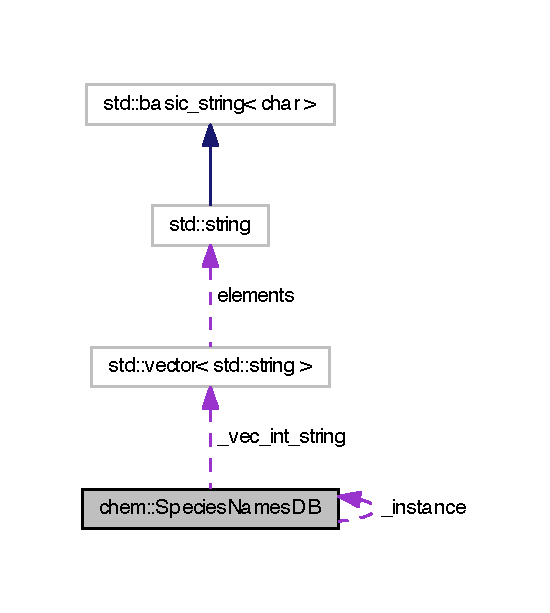
\includegraphics[width=264pt]{classchem_1_1SpeciesNamesDB__coll__graph}
\end{center}
\end{figure}
\subsection*{Public Member Functions}
\begin{DoxyCompactItemize}
\item 
std\-::string \hyperlink{classchem_1_1SpeciesNamesDB_ab4bd884d41961450ebe3d4d9564893a9}{int\-To\-String} (unsigned int i) const 
\begin{DoxyCompactList}\small\item\em Given an integer \char`\"{}i\char`\"{}, returns the std\-::string associated with that integer. Throws an out of range exception. \end{DoxyCompactList}\item 
int \hyperlink{classchem_1_1SpeciesNamesDB_acbb96b1e9cc8fee95c5b5f1b464cd5bd}{string\-To\-Int} (std\-::string name)
\begin{DoxyCompactList}\small\item\em Given a std\-::string \char`\"{}name\char`\"{}, returns the unique integer associated with that string. \end{DoxyCompactList}\item 
void \hyperlink{classchem_1_1SpeciesNamesDB_a08f8ec17dd512073c80ac83064d9f2b9}{clear} ()
\begin{DoxyCompactList}\small\item\em Clear the contents of the database. \end{DoxyCompactList}\end{DoxyCompactItemize}
\subsection*{Static Public Member Functions}
\begin{DoxyCompactItemize}
\item 
static \hyperlink{classchem_1_1SpeciesNamesDB}{Species\-Names\-D\-B} $\ast$ \hyperlink{classchem_1_1SpeciesNamesDB_af7921b9f52c8ed078718821bdb993109}{Instance} ()
\begin{DoxyCompactList}\small\item\em returns the unique instance of the singleton, which can be used to access the names D\-B \end{DoxyCompactList}\end{DoxyCompactItemize}
\subsection*{Private Member Functions}
\begin{DoxyCompactItemize}
\item 
\hyperlink{classchem_1_1SpeciesNamesDB_aaacfec3074bc2318a67fc86477f4d1fd}{Species\-Names\-D\-B} ()
\end{DoxyCompactItemize}
\subsection*{Private Attributes}
\begin{DoxyCompactItemize}
\item 
std\-::unordered\-\_\-map\\*
$<$ std\-::string, int $>$ \hyperlink{classchem_1_1SpeciesNamesDB_a2c70229e074e0997a876559ecb622fbb}{\-\_\-map\-\_\-string\-\_\-int}
\item 
std\-::vector$<$ std\-::string $>$ \hyperlink{classchem_1_1SpeciesNamesDB_ae9184194e3b6d35c36b43020bde04724}{\-\_\-vec\-\_\-int\-\_\-string}
\end{DoxyCompactItemize}
\subsection*{Static Private Attributes}
\begin{DoxyCompactItemize}
\item 
static \hyperlink{classchem_1_1SpeciesNamesDB}{Species\-Names\-D\-B} $\ast$ \hyperlink{classchem_1_1SpeciesNamesDB_a885f8676103893c462153cef1e47af0d}{\-\_\-instance} = 0
\begin{DoxyCompactList}\small\item\em the singleton instance \end{DoxyCompactList}\end{DoxyCompactItemize}


\subsection{Detailed Description}
\hyperlink{classchem_1_1SpeciesNamesDB}{Species\-Names\-D\-B} class is used to associate unique integers with character based names of \hyperlink{classchem_1_1Species}{Species}. 

Often \hyperlink{classchem_1_1Species}{Species} of the same type, let's say \char`\"{}\-Arp2/3\char`\"{} can be found in different forms, for example in cytosol vs bound to a filament. The corresponding specific \hyperlink{classchem_1_1Species}{Species} will be distinct, however, they will share the same name, as returned by \hyperlink{classchem_1_1Species_aa32c8f7fb344c68539a927c6a7f916c7}{Species\-::get\-Name()}. This, in turn, helps to match \char`\"{}\-Arp2/3\char`\"{} bound to filaments with diffusing \char`\"{}\-Arp2/3\char`\"{}. \hyperlink{classchem_1_1SpeciesNamesDB}{Species\-Names\-D\-B} associates a unique integer with \hyperlink{classchem_1_1Species}{Species} of the same type (e.\-g. \char`\"{}\-Arp2/3\char`\"{}, regardless whether it is bound or not), and provides conversion functions fron integer to std\-::string (Species\-Names\-D\-B\-::int\-To\-String(int i)) and vice versa (\hyperlink{classchem_1_1SpeciesNamesDB_acbb96b1e9cc8fee95c5b5f1b464cd5bd}{Species\-Names\-D\-B\-::string\-To\-Int} (std\-::string name)). class \hyperlink{classchem_1_1SpeciesNamesDB}{Species\-Names\-D\-B} is a singleton, and should be used by first calling \hyperlink{classchem_1_1SpeciesNamesDB_af7921b9f52c8ed078718821bdb993109}{Species\-Names\-D\-B\-::\-Instance()} method.


\begin{DoxyCode}
  int y = SpeciesNamesDB::Instance()->stringToInt("Arp2/3"); // let's say y=2
  std::string x = SpeciesNamesDB::Instance()->intToString(2); // then x should
       be "Arp2/3"
\end{DoxyCode}
 

Definition at line 54 of file Species.\-h.



\subsection{Constructor \& Destructor Documentation}
\hypertarget{classchem_1_1SpeciesNamesDB_aaacfec3074bc2318a67fc86477f4d1fd}{\index{chem\-::\-Species\-Names\-D\-B@{chem\-::\-Species\-Names\-D\-B}!Species\-Names\-D\-B@{Species\-Names\-D\-B}}
\index{Species\-Names\-D\-B@{Species\-Names\-D\-B}!chem::SpeciesNamesDB@{chem\-::\-Species\-Names\-D\-B}}
\subsubsection[{Species\-Names\-D\-B}]{\setlength{\rightskip}{0pt plus 5cm}{\bf chem\-::\-Species\-Names\-D\-B\-::\-Species\-Names\-D\-B} (
\begin{DoxyParamCaption}
{}
\end{DoxyParamCaption}
)\hspace{0.3cm}{\ttfamily  \mbox{[}inline, private\mbox{]}}}}\label{classchem_1_1SpeciesNamesDB_aaacfec3074bc2318a67fc86477f4d1fd}


Definition at line 57 of file Species.\-h.



Referenced by Instance().



\subsection{Member Function Documentation}
\hypertarget{classchem_1_1SpeciesNamesDB_a08f8ec17dd512073c80ac83064d9f2b9}{\index{chem\-::\-Species\-Names\-D\-B@{chem\-::\-Species\-Names\-D\-B}!clear@{clear}}
\index{clear@{clear}!chem::SpeciesNamesDB@{chem\-::\-Species\-Names\-D\-B}}
\subsubsection[{clear}]{\setlength{\rightskip}{0pt plus 5cm}void {\bf chem\-::\-Species\-Names\-D\-B\-::clear} (
\begin{DoxyParamCaption}
{}
\end{DoxyParamCaption}
)\hspace{0.3cm}{\ttfamily  \mbox{[}inline\mbox{]}}}}\label{classchem_1_1SpeciesNamesDB_a08f8ec17dd512073c80ac83064d9f2b9}


Clear the contents of the database. 



Definition at line 86 of file Species.\-h.



References \-\_\-map\-\_\-string\-\_\-int, and \-\_\-vec\-\_\-int\-\_\-string.

\hypertarget{classchem_1_1SpeciesNamesDB_af7921b9f52c8ed078718821bdb993109}{\index{chem\-::\-Species\-Names\-D\-B@{chem\-::\-Species\-Names\-D\-B}!Instance@{Instance}}
\index{Instance@{Instance}!chem::SpeciesNamesDB@{chem\-::\-Species\-Names\-D\-B}}
\subsubsection[{Instance}]{\setlength{\rightskip}{0pt plus 5cm}{\bf Species\-Names\-D\-B} $\ast$ {\bf chem\-::\-Species\-Names\-D\-B\-::\-Instance} (
\begin{DoxyParamCaption}
{}
\end{DoxyParamCaption}
)\hspace{0.3cm}{\ttfamily  \mbox{[}static\mbox{]}}}}\label{classchem_1_1SpeciesNamesDB_af7921b9f52c8ed078718821bdb993109}


returns the unique instance of the singleton, which can be used to access the names D\-B 



Definition at line 20 of file Species.\-cpp.



References \-\_\-instance, and Species\-Names\-D\-B().



Referenced by chem\-::\-Species\-::get\-Name(), chem\-::\-Compartment\-::set\-Diffusion\-Rate(), and chem\-::\-Species\-::\-Species().

\hypertarget{classchem_1_1SpeciesNamesDB_ab4bd884d41961450ebe3d4d9564893a9}{\index{chem\-::\-Species\-Names\-D\-B@{chem\-::\-Species\-Names\-D\-B}!int\-To\-String@{int\-To\-String}}
\index{int\-To\-String@{int\-To\-String}!chem::SpeciesNamesDB@{chem\-::\-Species\-Names\-D\-B}}
\subsubsection[{int\-To\-String}]{\setlength{\rightskip}{0pt plus 5cm}std\-::string {\bf chem\-::\-Species\-Names\-D\-B\-::int\-To\-String} (
\begin{DoxyParamCaption}
\item[{unsigned int}]{i}
\end{DoxyParamCaption}
) const\hspace{0.3cm}{\ttfamily  \mbox{[}inline\mbox{]}}}}\label{classchem_1_1SpeciesNamesDB_ab4bd884d41961450ebe3d4d9564893a9}


Given an integer \char`\"{}i\char`\"{}, returns the std\-::string associated with that integer. Throws an out of range exception. 



Definition at line 66 of file Species.\-h.



References \-\_\-vec\-\_\-int\-\_\-string.



Referenced by chem\-::\-Species\-::get\-Name().

\hypertarget{classchem_1_1SpeciesNamesDB_acbb96b1e9cc8fee95c5b5f1b464cd5bd}{\index{chem\-::\-Species\-Names\-D\-B@{chem\-::\-Species\-Names\-D\-B}!string\-To\-Int@{string\-To\-Int}}
\index{string\-To\-Int@{string\-To\-Int}!chem::SpeciesNamesDB@{chem\-::\-Species\-Names\-D\-B}}
\subsubsection[{string\-To\-Int}]{\setlength{\rightskip}{0pt plus 5cm}int {\bf chem\-::\-Species\-Names\-D\-B\-::string\-To\-Int} (
\begin{DoxyParamCaption}
\item[{std\-::string}]{name}
\end{DoxyParamCaption}
)\hspace{0.3cm}{\ttfamily  \mbox{[}inline\mbox{]}}}}\label{classchem_1_1SpeciesNamesDB_acbb96b1e9cc8fee95c5b5f1b464cd5bd}


Given a std\-::string \char`\"{}name\char`\"{}, returns the unique integer associated with that string. 

If the string does not exist yet, it is created. 

Definition at line 74 of file Species.\-h.



References \-\_\-map\-\_\-string\-\_\-int, and \-\_\-vec\-\_\-int\-\_\-string.



Referenced by chem\-::\-Compartment\-::set\-Diffusion\-Rate(), and chem\-::\-Species\-::\-Species().



\subsection{Member Data Documentation}
\hypertarget{classchem_1_1SpeciesNamesDB_a885f8676103893c462153cef1e47af0d}{\index{chem\-::\-Species\-Names\-D\-B@{chem\-::\-Species\-Names\-D\-B}!\-\_\-instance@{\-\_\-instance}}
\index{\-\_\-instance@{\-\_\-instance}!chem::SpeciesNamesDB@{chem\-::\-Species\-Names\-D\-B}}
\subsubsection[{\-\_\-instance}]{\setlength{\rightskip}{0pt plus 5cm}{\bf Species\-Names\-D\-B} $\ast$ {\bf chem\-::\-Species\-Names\-D\-B\-::\-\_\-instance} = 0\hspace{0.3cm}{\ttfamily  \mbox{[}static, private\mbox{]}}}}\label{classchem_1_1SpeciesNamesDB_a885f8676103893c462153cef1e47af0d}


the singleton instance 



Definition at line 56 of file Species.\-h.



Referenced by Instance().

\hypertarget{classchem_1_1SpeciesNamesDB_a2c70229e074e0997a876559ecb622fbb}{\index{chem\-::\-Species\-Names\-D\-B@{chem\-::\-Species\-Names\-D\-B}!\-\_\-map\-\_\-string\-\_\-int@{\-\_\-map\-\_\-string\-\_\-int}}
\index{\-\_\-map\-\_\-string\-\_\-int@{\-\_\-map\-\_\-string\-\_\-int}!chem::SpeciesNamesDB@{chem\-::\-Species\-Names\-D\-B}}
\subsubsection[{\-\_\-map\-\_\-string\-\_\-int}]{\setlength{\rightskip}{0pt plus 5cm}std\-::unordered\-\_\-map$<$std\-::string,int$>$ {\bf chem\-::\-Species\-Names\-D\-B\-::\-\_\-map\-\_\-string\-\_\-int}\hspace{0.3cm}{\ttfamily  \mbox{[}private\mbox{]}}}}\label{classchem_1_1SpeciesNamesDB_a2c70229e074e0997a876559ecb622fbb}


Definition at line 59 of file Species.\-h.



Referenced by clear(), and string\-To\-Int().

\hypertarget{classchem_1_1SpeciesNamesDB_ae9184194e3b6d35c36b43020bde04724}{\index{chem\-::\-Species\-Names\-D\-B@{chem\-::\-Species\-Names\-D\-B}!\-\_\-vec\-\_\-int\-\_\-string@{\-\_\-vec\-\_\-int\-\_\-string}}
\index{\-\_\-vec\-\_\-int\-\_\-string@{\-\_\-vec\-\_\-int\-\_\-string}!chem::SpeciesNamesDB@{chem\-::\-Species\-Names\-D\-B}}
\subsubsection[{\-\_\-vec\-\_\-int\-\_\-string}]{\setlength{\rightskip}{0pt plus 5cm}std\-::vector$<$std\-::string$>$ {\bf chem\-::\-Species\-Names\-D\-B\-::\-\_\-vec\-\_\-int\-\_\-string}\hspace{0.3cm}{\ttfamily  \mbox{[}private\mbox{]}}}}\label{classchem_1_1SpeciesNamesDB_ae9184194e3b6d35c36b43020bde04724}


Definition at line 60 of file Species.\-h.



Referenced by clear(), int\-To\-String(), and string\-To\-Int().



The documentation for this class was generated from the following files\-:\begin{DoxyCompactItemize}
\item 
Cyto\-Sim/\hyperlink{Species_8h}{Species.\-h}\item 
Cyto\-Sim/\hyperlink{Species_8cpp}{Species.\-cpp}\end{DoxyCompactItemize}

\input{classchem_1_1SpeciesPtrContainerIFace}
\input{classchem_1_1SpeciesPtrContainerVector}
\hypertarget{classSystem}{\section{System Class Reference}
\label{classSystem}\index{System@{System}}
}


{\ttfamily \#include $<$System.\-h$>$}



Collaboration diagram for System\-:
\nopagebreak
\begin{figure}[H]
\begin{center}
\leavevmode
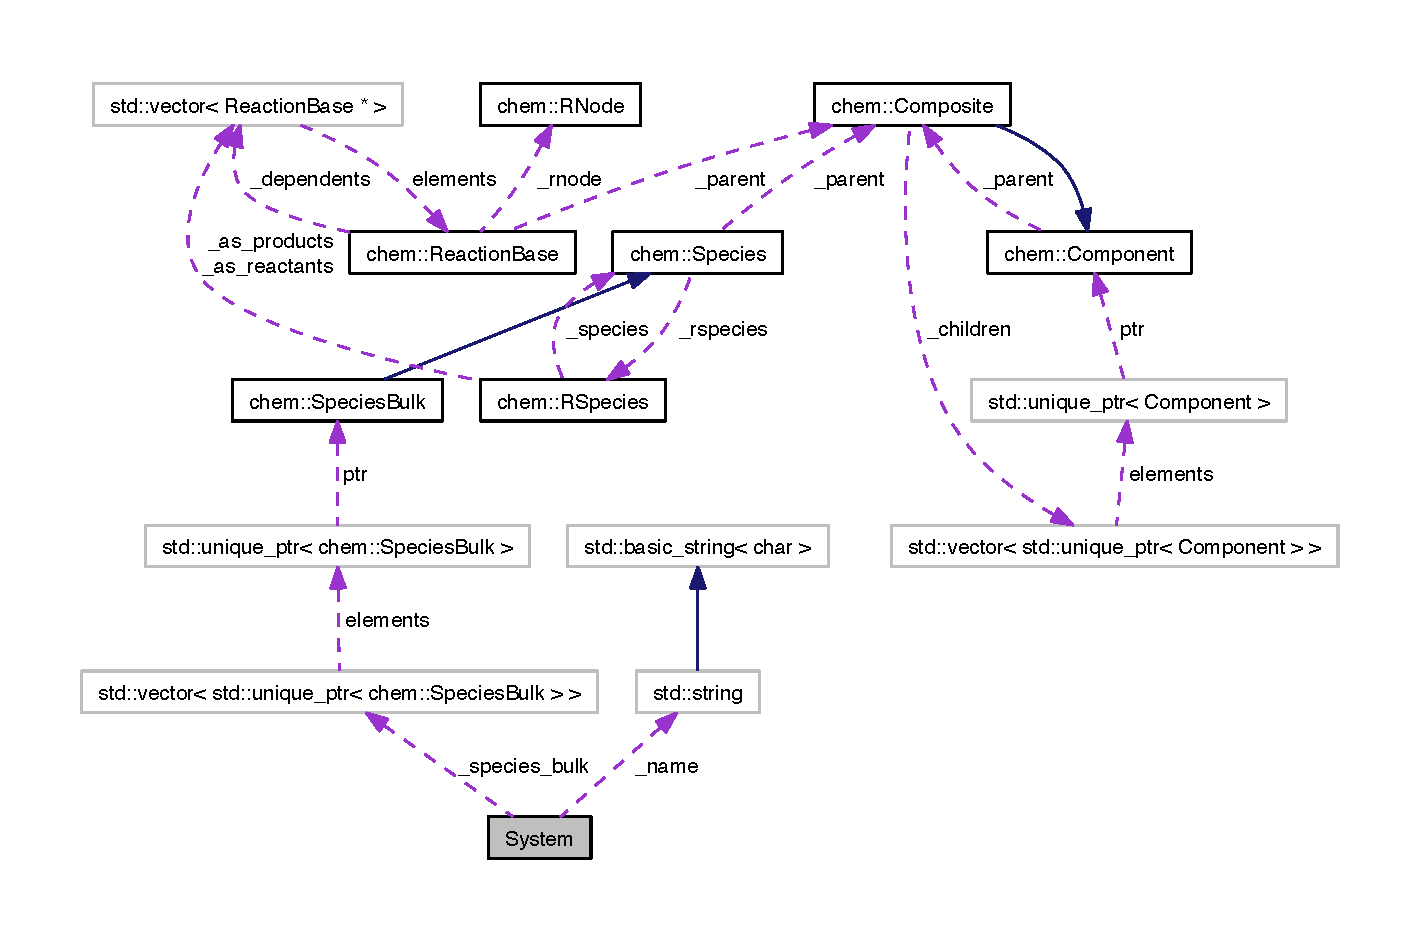
\includegraphics[width=350pt]{classSystem__coll__graph}
\end{center}
\end{figure}
\subsection*{Public Member Functions}
\begin{DoxyCompactItemize}
\item 
void \hyperlink{classSystem_a6f4360b4a491316bc77e6c310cdf6512}{set\-Name} (const std\-::string \&name)
\item 
std\-::string \hyperlink{classSystem_a774d78ae771d47f38d09c288298f936a}{get\-Name} () const 
\item 
\hyperlink{classchem_1_1SpeciesBulk}{chem\-::\-Species\-Bulk} $\ast$ \hyperlink{classSystem_a141acd0fd533f36a1ae9e12b6b8ecda7}{add\-Species\-Bulk} (const std\-::string name, \hyperlink{common_8h_a3503f321fd36304ee274141275cca586}{species\-\_\-copy\-\_\-t} n=0)
\end{DoxyCompactItemize}
\subsection*{Private Attributes}
\begin{DoxyCompactItemize}
\item 
std\-::vector$<$ std\-::unique\-\_\-ptr\\*
$<$ \hyperlink{classchem_1_1SpeciesBulk}{chem\-::\-Species\-Bulk} $>$ $>$ \hyperlink{classSystem_a58cada67a766fc38e52ed4abfd373486}{\-\_\-species\-\_\-bulk}
\item 
std\-::string \hyperlink{classSystem_a096b362d79b514fee041ff52259642d3}{\-\_\-name}
\begin{DoxyCompactList}\small\item\em \hyperlink{classSystem}{System}'s name. \end{DoxyCompactList}\end{DoxyCompactItemize}


\subsection{Detailed Description}


Definition at line 17 of file System.\-h.



\subsection{Member Function Documentation}
\hypertarget{classSystem_a141acd0fd533f36a1ae9e12b6b8ecda7}{\index{System@{System}!add\-Species\-Bulk@{add\-Species\-Bulk}}
\index{add\-Species\-Bulk@{add\-Species\-Bulk}!System@{System}}
\subsubsection[{add\-Species\-Bulk}]{\setlength{\rightskip}{0pt plus 5cm}{\bf chem\-::\-Species\-Bulk}$\ast$ {\bf System\-::add\-Species\-Bulk} (
\begin{DoxyParamCaption}
\item[{const std\-::string}]{name, }
\item[{{\bf species\-\_\-copy\-\_\-t}}]{n = {\ttfamily 0}}
\end{DoxyParamCaption}
)\hspace{0.3cm}{\ttfamily  \mbox{[}inline\mbox{]}}}}\label{classSystem_a141acd0fd533f36a1ae9e12b6b8ecda7}


Definition at line 21 of file System.\-h.



References \-\_\-species\-\_\-bulk.

\hypertarget{classSystem_a774d78ae771d47f38d09c288298f936a}{\index{System@{System}!get\-Name@{get\-Name}}
\index{get\-Name@{get\-Name}!System@{System}}
\subsubsection[{get\-Name}]{\setlength{\rightskip}{0pt plus 5cm}std\-::string {\bf System\-::get\-Name} (
\begin{DoxyParamCaption}
{}
\end{DoxyParamCaption}
) const\hspace{0.3cm}{\ttfamily  \mbox{[}inline\mbox{]}}}}\label{classSystem_a774d78ae771d47f38d09c288298f936a}


Definition at line 20 of file System.\-h.



References \-\_\-name.

\hypertarget{classSystem_a6f4360b4a491316bc77e6c310cdf6512}{\index{System@{System}!set\-Name@{set\-Name}}
\index{set\-Name@{set\-Name}!System@{System}}
\subsubsection[{set\-Name}]{\setlength{\rightskip}{0pt plus 5cm}void {\bf System\-::set\-Name} (
\begin{DoxyParamCaption}
\item[{const std\-::string \&}]{name}
\end{DoxyParamCaption}
)\hspace{0.3cm}{\ttfamily  \mbox{[}inline\mbox{]}}}}\label{classSystem_a6f4360b4a491316bc77e6c310cdf6512}


Definition at line 19 of file System.\-h.



References \-\_\-name.



\subsection{Member Data Documentation}
\hypertarget{classSystem_a096b362d79b514fee041ff52259642d3}{\index{System@{System}!\-\_\-name@{\-\_\-name}}
\index{\-\_\-name@{\-\_\-name}!System@{System}}
\subsubsection[{\-\_\-name}]{\setlength{\rightskip}{0pt plus 5cm}std\-::string {\bf System\-::\-\_\-name}\hspace{0.3cm}{\ttfamily  \mbox{[}private\mbox{]}}}}\label{classSystem_a096b362d79b514fee041ff52259642d3}


\hyperlink{classSystem}{System}'s name. 



Definition at line 27 of file System.\-h.



Referenced by get\-Name(), and set\-Name().

\hypertarget{classSystem_a58cada67a766fc38e52ed4abfd373486}{\index{System@{System}!\-\_\-species\-\_\-bulk@{\-\_\-species\-\_\-bulk}}
\index{\-\_\-species\-\_\-bulk@{\-\_\-species\-\_\-bulk}!System@{System}}
\subsubsection[{\-\_\-species\-\_\-bulk}]{\setlength{\rightskip}{0pt plus 5cm}std\-::vector$<$std\-::unique\-\_\-ptr$<${\bf chem\-::\-Species\-Bulk}$>$ $>$ {\bf System\-::\-\_\-species\-\_\-bulk}\hspace{0.3cm}{\ttfamily  \mbox{[}private\mbox{]}}}}\label{classSystem_a58cada67a766fc38e52ed4abfd373486}


Definition at line 26 of file System.\-h.



Referenced by add\-Species\-Bulk().



The documentation for this class was generated from the following file\-:\begin{DoxyCompactItemize}
\item 
Cyto\-Sim/\hyperlink{System_8h}{System.\-h}\end{DoxyCompactItemize}

\hypertarget{classchem_1_1Visitor}{\section{chem\-:\-:Visitor Class Reference}
\label{classchem_1_1Visitor}\index{chem\-::\-Visitor@{chem\-::\-Visitor}}
}


{\ttfamily \#include $<$Visitor.\-h$>$}



Inheritance diagram for chem\-:\-:Visitor\-:\nopagebreak
\begin{figure}[H]
\begin{center}
\leavevmode
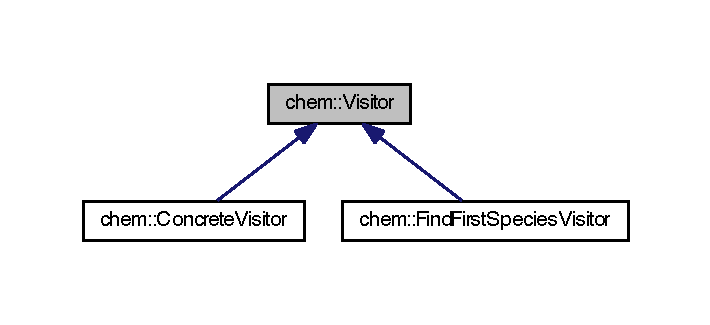
\includegraphics[width=341pt]{classchem_1_1Visitor__inherit__graph}
\end{center}
\end{figure}
\subsection*{Public Member Functions}
\begin{DoxyCompactItemize}
\item 
virtual bool \hyperlink{classchem_1_1Visitor_a3a148d3144ed2ef25972509a6a594d1a}{visit} (\hyperlink{classchem_1_1Component}{Component} $\ast$c)=0
\item 
virtual \hyperlink{classchem_1_1Visitor_a1f8b4dc62e90ed58f0b53e906a782ee0}{$\sim$\-Visitor} ()
\end{DoxyCompactItemize}


\subsection{Detailed Description}


Definition at line 17 of file Visitor.\-h.



\subsection{Constructor \& Destructor Documentation}
\hypertarget{classchem_1_1Visitor_a1f8b4dc62e90ed58f0b53e906a782ee0}{\index{chem\-::\-Visitor@{chem\-::\-Visitor}!$\sim$\-Visitor@{$\sim$\-Visitor}}
\index{$\sim$\-Visitor@{$\sim$\-Visitor}!chem::Visitor@{chem\-::\-Visitor}}
\subsubsection[{$\sim$\-Visitor}]{\setlength{\rightskip}{0pt plus 5cm}virtual {\bf chem\-::\-Visitor\-::$\sim$\-Visitor} (
\begin{DoxyParamCaption}
{}
\end{DoxyParamCaption}
)\hspace{0.3cm}{\ttfamily  \mbox{[}inline, virtual\mbox{]}}}}\label{classchem_1_1Visitor_a1f8b4dc62e90ed58f0b53e906a782ee0}


Definition at line 20 of file Visitor.\-h.



\subsection{Member Function Documentation}
\hypertarget{classchem_1_1Visitor_a3a148d3144ed2ef25972509a6a594d1a}{\index{chem\-::\-Visitor@{chem\-::\-Visitor}!visit@{visit}}
\index{visit@{visit}!chem::Visitor@{chem\-::\-Visitor}}
\subsubsection[{visit}]{\setlength{\rightskip}{0pt plus 5cm}virtual bool {\bf chem\-::\-Visitor\-::visit} (
\begin{DoxyParamCaption}
\item[{{\bf Component} $\ast$}]{c}
\end{DoxyParamCaption}
)\hspace{0.3cm}{\ttfamily  \mbox{[}pure virtual\mbox{]}}}}\label{classchem_1_1Visitor_a3a148d3144ed2ef25972509a6a594d1a}


Implemented in \hyperlink{classchem_1_1FindFirstSpeciesVisitor_afe2b8f520e443307a6ba06a24c4b9991}{chem\-::\-Find\-First\-Species\-Visitor}, and \hyperlink{classchem_1_1ConcreteVisitor_abb5892cdcf90fef25aafafaf81baa697}{chem\-::\-Concrete\-Visitor}.



Referenced by chem\-::\-Component\-::apply(), and chem\-::\-Composite\-::apply().



The documentation for this class was generated from the following file\-:\begin{DoxyCompactItemize}
\item 
Cyto\-Sim/\hyperlink{Visitor_8h}{Visitor.\-h}\end{DoxyCompactItemize}

\chapter{File Documentation}
\hypertarget{ChemGillespieImpl_8cpp}{\section{M3\+S\+Y\+M/\+Chemistry/\+Chem\+Gillespie\+Impl.cpp File Reference}
\label{ChemGillespieImpl_8cpp}\index{M3\+S\+Y\+M/\+Chemistry/\+Chem\+Gillespie\+Impl.\+cpp@{M3\+S\+Y\+M/\+Chemistry/\+Chem\+Gillespie\+Impl.\+cpp}}
}
{\ttfamily \#include \char`\"{}Chem\+Gillespie\+Impl.\+h\char`\"{}}\\*
Include dependency graph for Chem\+Gillespie\+Impl.\+cpp\+:\nopagebreak
\begin{figure}[H]
\begin{center}
\leavevmode
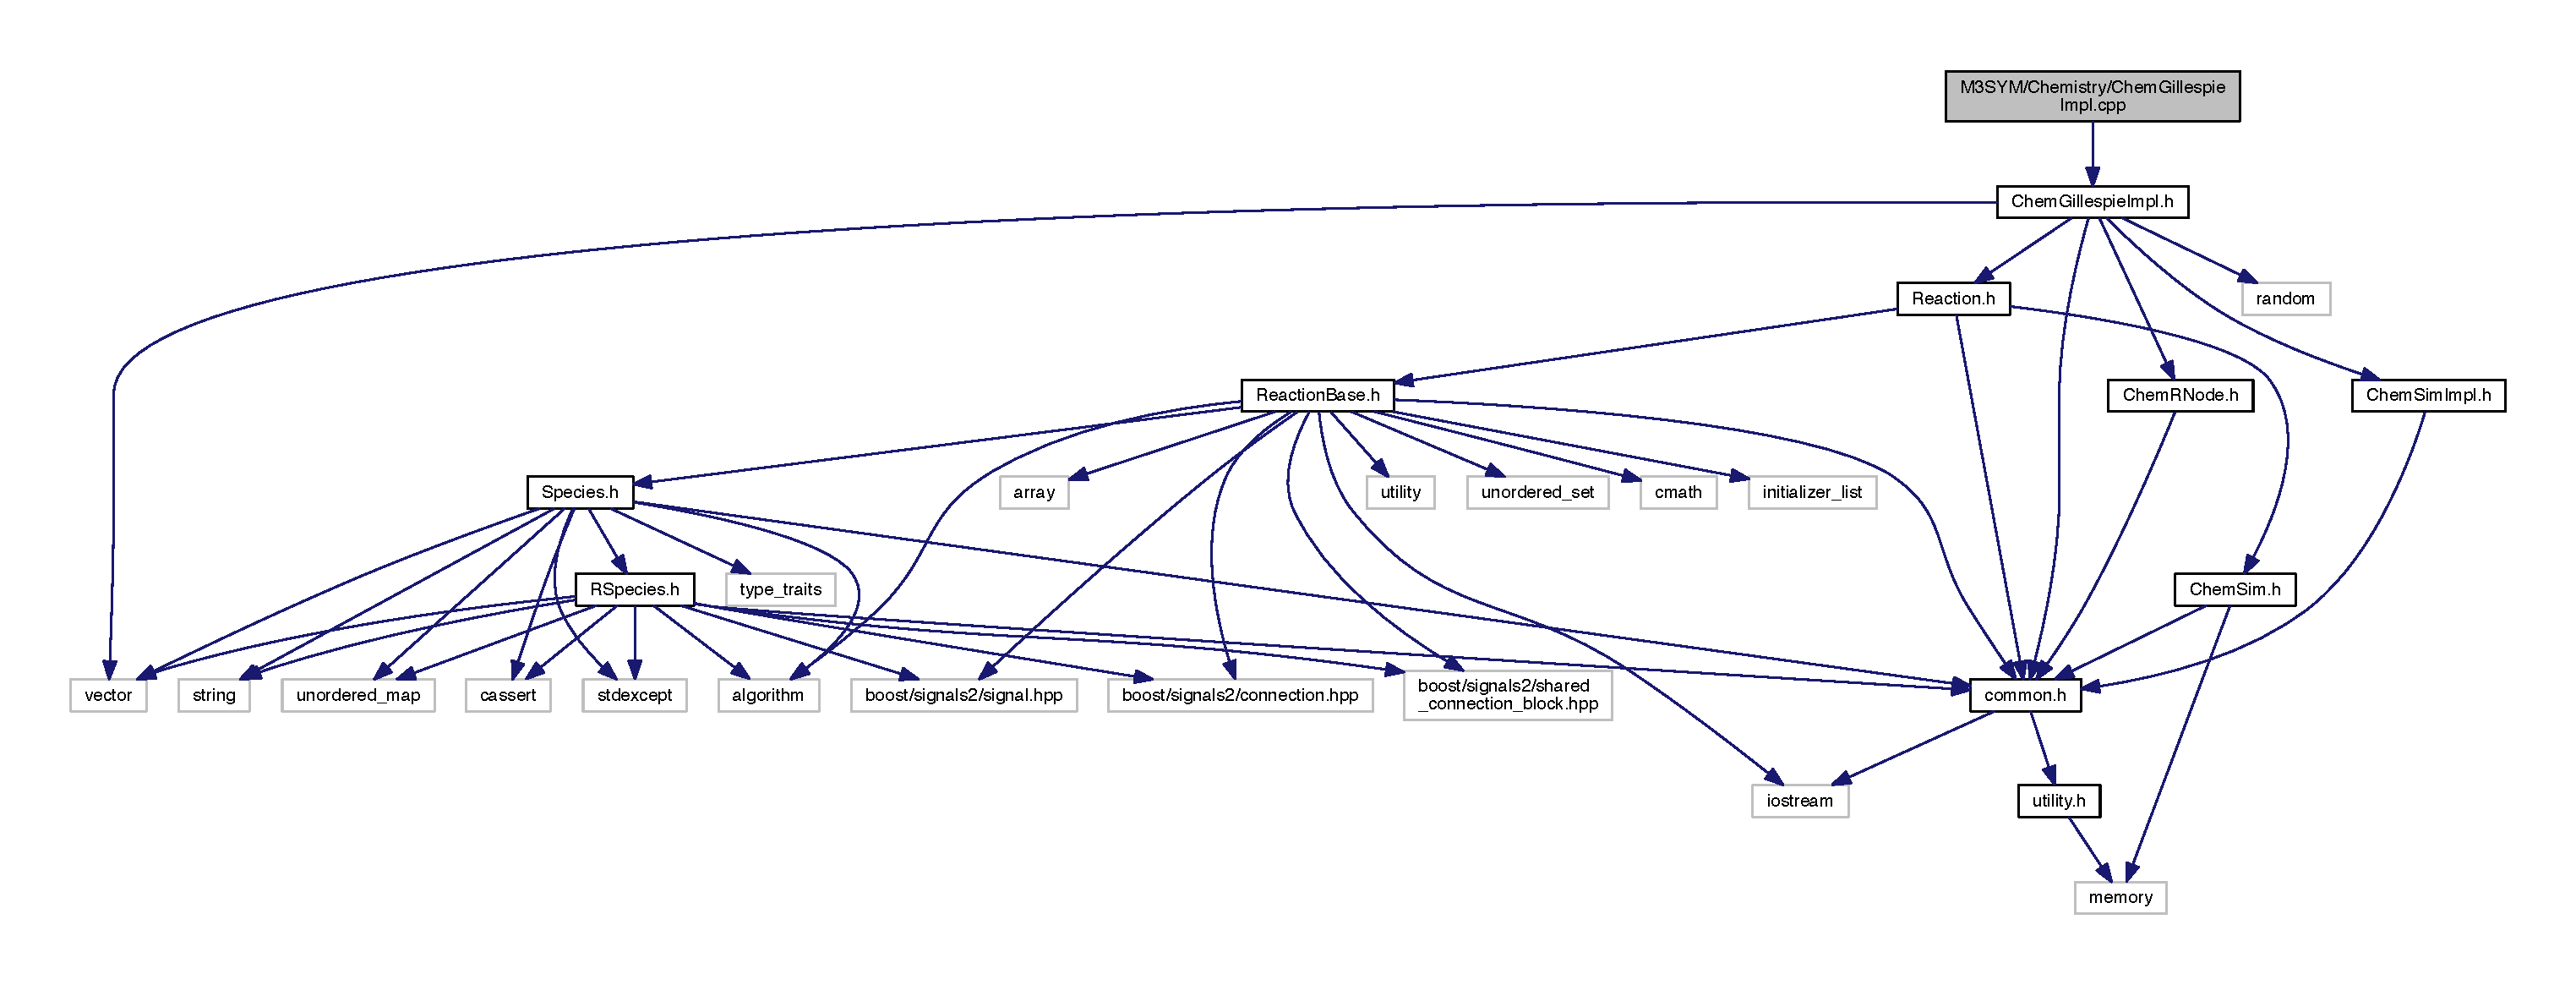
\includegraphics[width=350pt]{ChemGillespieImpl_8cpp__incl}
\end{center}
\end{figure}

\hypertarget{ChemGillespieImpl_8h}{\section{M3\+S\+Y\+M/\+Chemistry/\+Chem\+Gillespie\+Impl.h File Reference}
\label{ChemGillespieImpl_8h}\index{M3\+S\+Y\+M/\+Chemistry/\+Chem\+Gillespie\+Impl.\+h@{M3\+S\+Y\+M/\+Chemistry/\+Chem\+Gillespie\+Impl.\+h}}
}
{\ttfamily \#include $<$vector$>$}\\*
{\ttfamily \#include $<$random$>$}\\*
{\ttfamily \#include \char`\"{}common.\+h\char`\"{}}\\*
{\ttfamily \#include \char`\"{}Reaction.\+h\char`\"{}}\\*
{\ttfamily \#include \char`\"{}Chem\+R\+Node.\+h\char`\"{}}\\*
{\ttfamily \#include \char`\"{}Chem\+Sim\+Impl.\+h\char`\"{}}\\*
Include dependency graph for Chem\+Gillespie\+Impl.\+h\+:\nopagebreak
\begin{figure}[H]
\begin{center}
\leavevmode
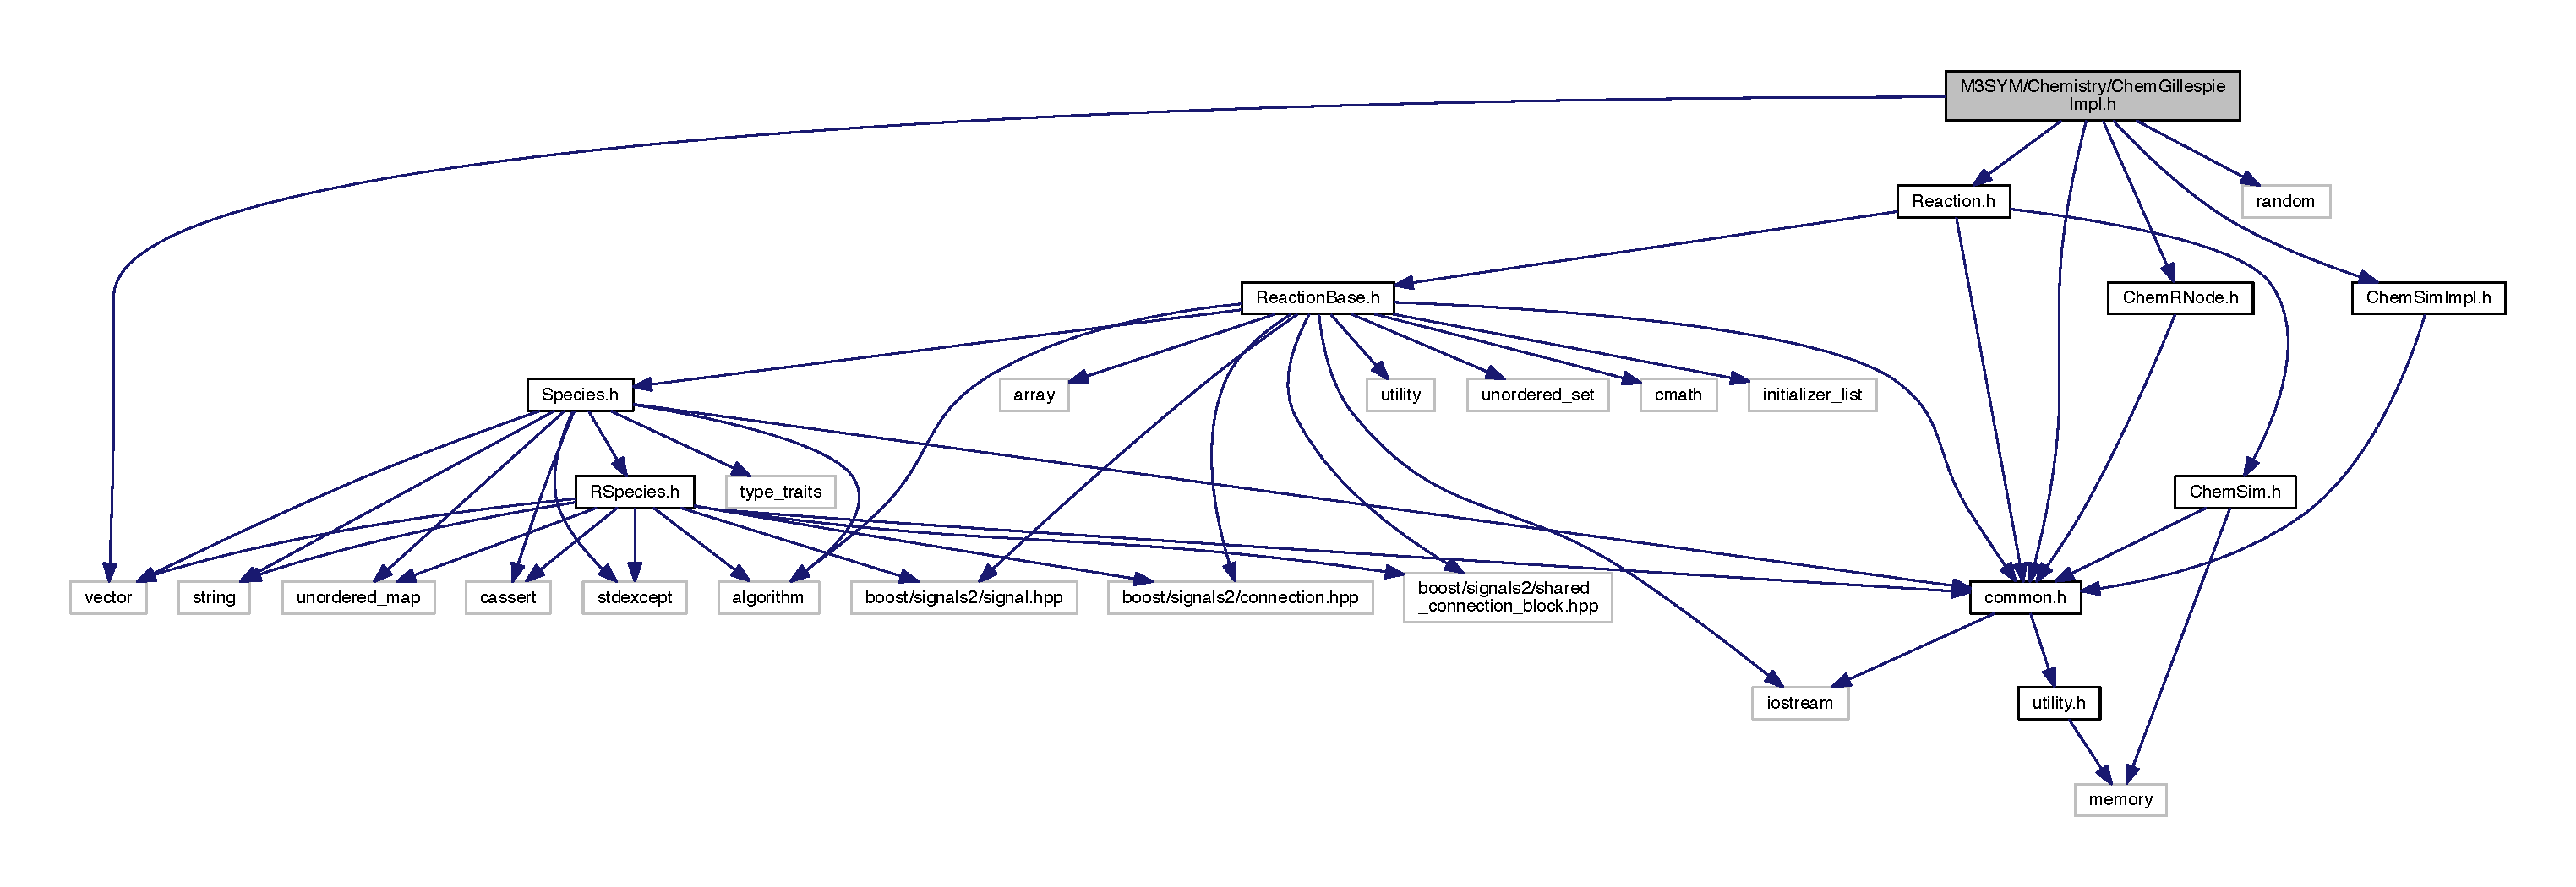
\includegraphics[width=350pt]{ChemGillespieImpl_8h__incl}
\end{center}
\end{figure}
This graph shows which files directly or indirectly include this file\+:\nopagebreak
\begin{figure}[H]
\begin{center}
\leavevmode
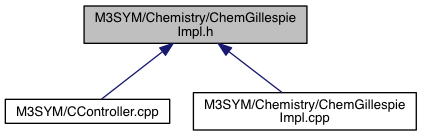
\includegraphics[width=350pt]{ChemGillespieImpl_8h__dep__incl}
\end{center}
\end{figure}
\subsection*{Classes}
\begin{DoxyCompactItemize}
\item 
class \hyperlink{classRNodeGillespie}{R\+Node\+Gillespie}
\begin{DoxyCompactList}\small\item\em Used by \hyperlink{classChemGillespieImpl}{Chem\+Gillespie\+Impl} to implement the cached version of the Gillespie algorithm. \end{DoxyCompactList}\item 
class \hyperlink{classChemGillespieImpl}{Chem\+Gillespie\+Impl}
\begin{DoxyCompactList}\small\item\em Implements a slightly optimized version of the Gillespie algorithm. \end{DoxyCompactList}\end{DoxyCompactItemize}

\hypertarget{ChemNRMImpl_8cpp}{\section{Cyto\-Sim/\-Chem\-N\-R\-M\-Impl.cpp File Reference}
\label{ChemNRMImpl_8cpp}\index{Cyto\-Sim/\-Chem\-N\-R\-M\-Impl.\-cpp@{Cyto\-Sim/\-Chem\-N\-R\-M\-Impl.\-cpp}}
}
{\ttfamily \#include $<$iostream$>$}\\*
{\ttfamily \#include \char`\"{}Chem\-N\-R\-M\-Impl.\-h\char`\"{}}\\*
Include dependency graph for Chem\-N\-R\-M\-Impl.\-cpp\-:\nopagebreak
\begin{figure}[H]
\begin{center}
\leavevmode
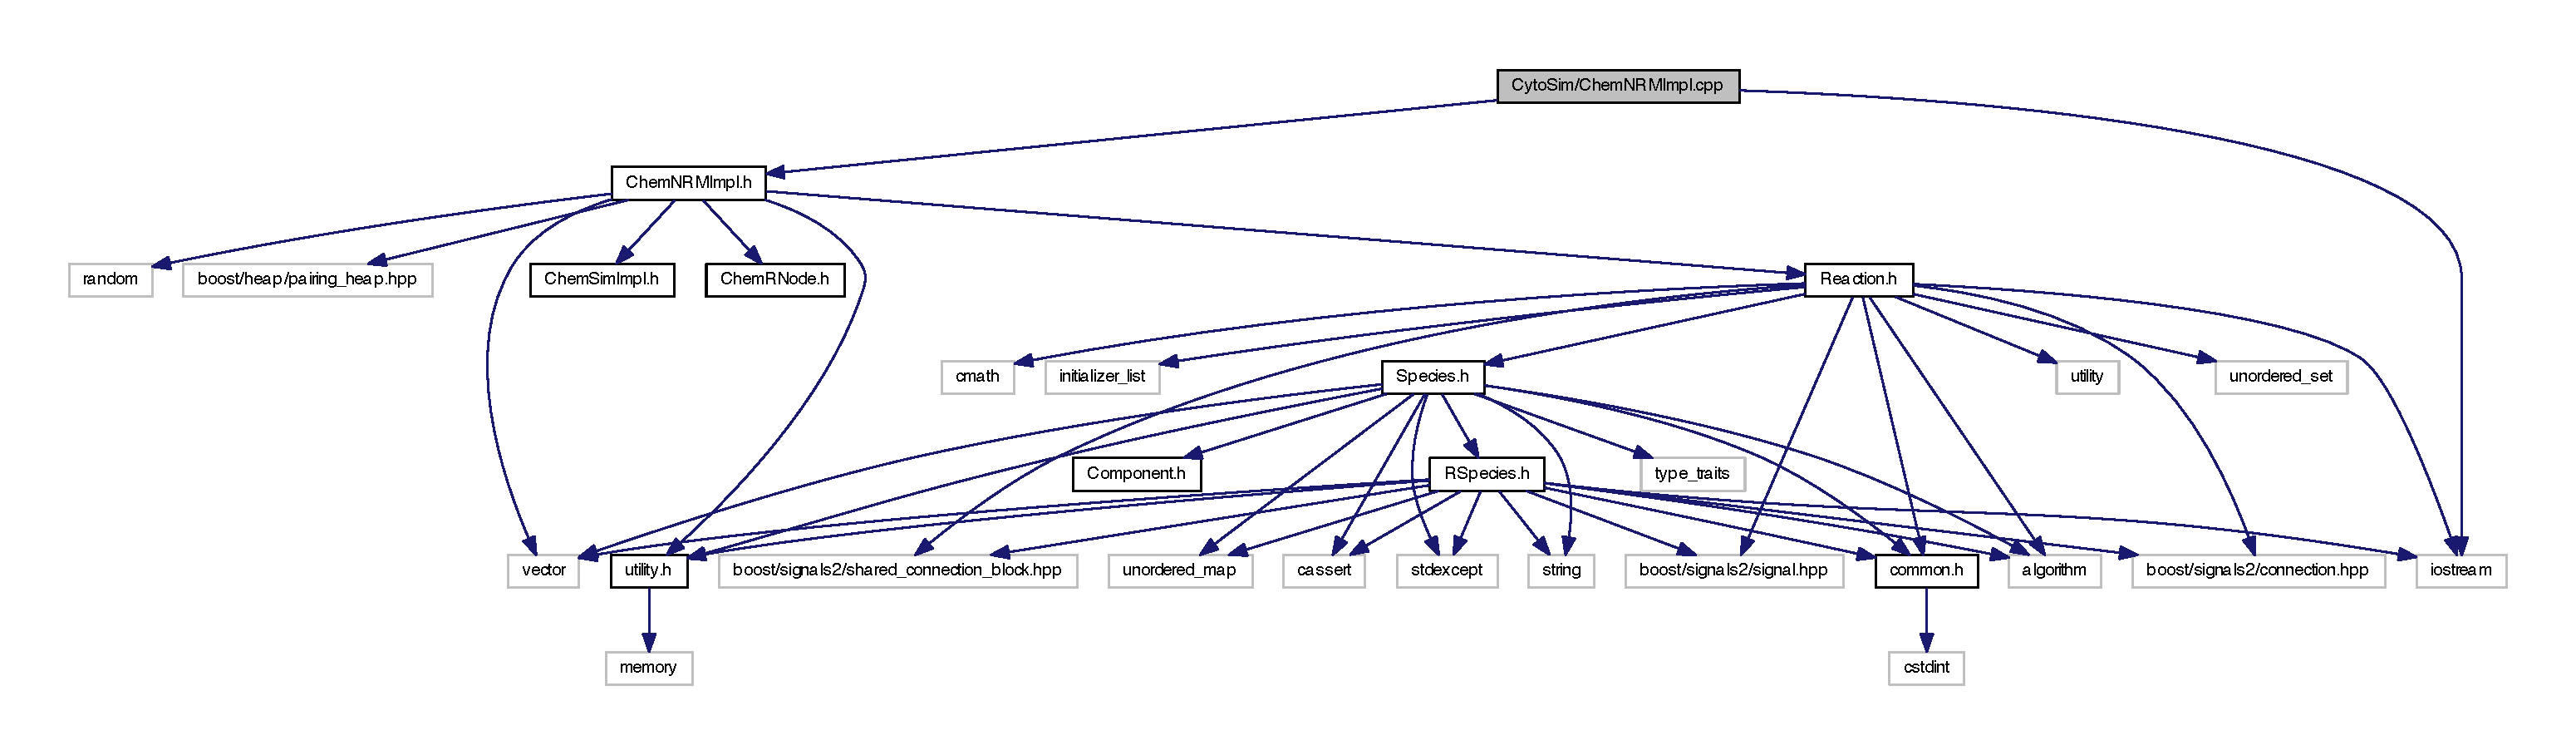
\includegraphics[width=350pt]{ChemNRMImpl_8cpp__incl}
\end{center}
\end{figure}
\subsection*{Namespaces}
\begin{DoxyCompactItemize}
\item 
namespace \hyperlink{namespacechem}{chem}
\begin{DoxyCompactList}\small\item\em The algorithm implemented here is based on the following reference\-: $\ast$$\ast$ Michael A. Gibson, and Jehoshua Bruck J. Phys. Chem. A, 2000, 104 (9), 1876-\/1889 $\ast$$\ast$. \end{DoxyCompactList}\end{DoxyCompactItemize}

\hypertarget{ChemNRMImpl_8h}{\section{M3\+S\+Y\+M/\+Chemistry/\+Chem\+N\+R\+M\+Impl.h File Reference}
\label{ChemNRMImpl_8h}\index{M3\+S\+Y\+M/\+Chemistry/\+Chem\+N\+R\+M\+Impl.\+h@{M3\+S\+Y\+M/\+Chemistry/\+Chem\+N\+R\+M\+Impl.\+h}}
}
{\ttfamily \#include $<$vector$>$}\\*
{\ttfamily \#include $<$random$>$}\\*
{\ttfamily \#include $<$boost/heap/pairing\+\_\+heap.\+hpp$>$}\\*
{\ttfamily \#include \char`\"{}common.\+h\char`\"{}}\\*
{\ttfamily \#include \char`\"{}Reaction.\+h\char`\"{}}\\*
{\ttfamily \#include \char`\"{}Chem\+Sim\+Impl.\+h\char`\"{}}\\*
{\ttfamily \#include \char`\"{}Chem\+R\+Node.\+h\char`\"{}}\\*
Include dependency graph for Chem\+N\+R\+M\+Impl.\+h\+:\nopagebreak
\begin{figure}[H]
\begin{center}
\leavevmode
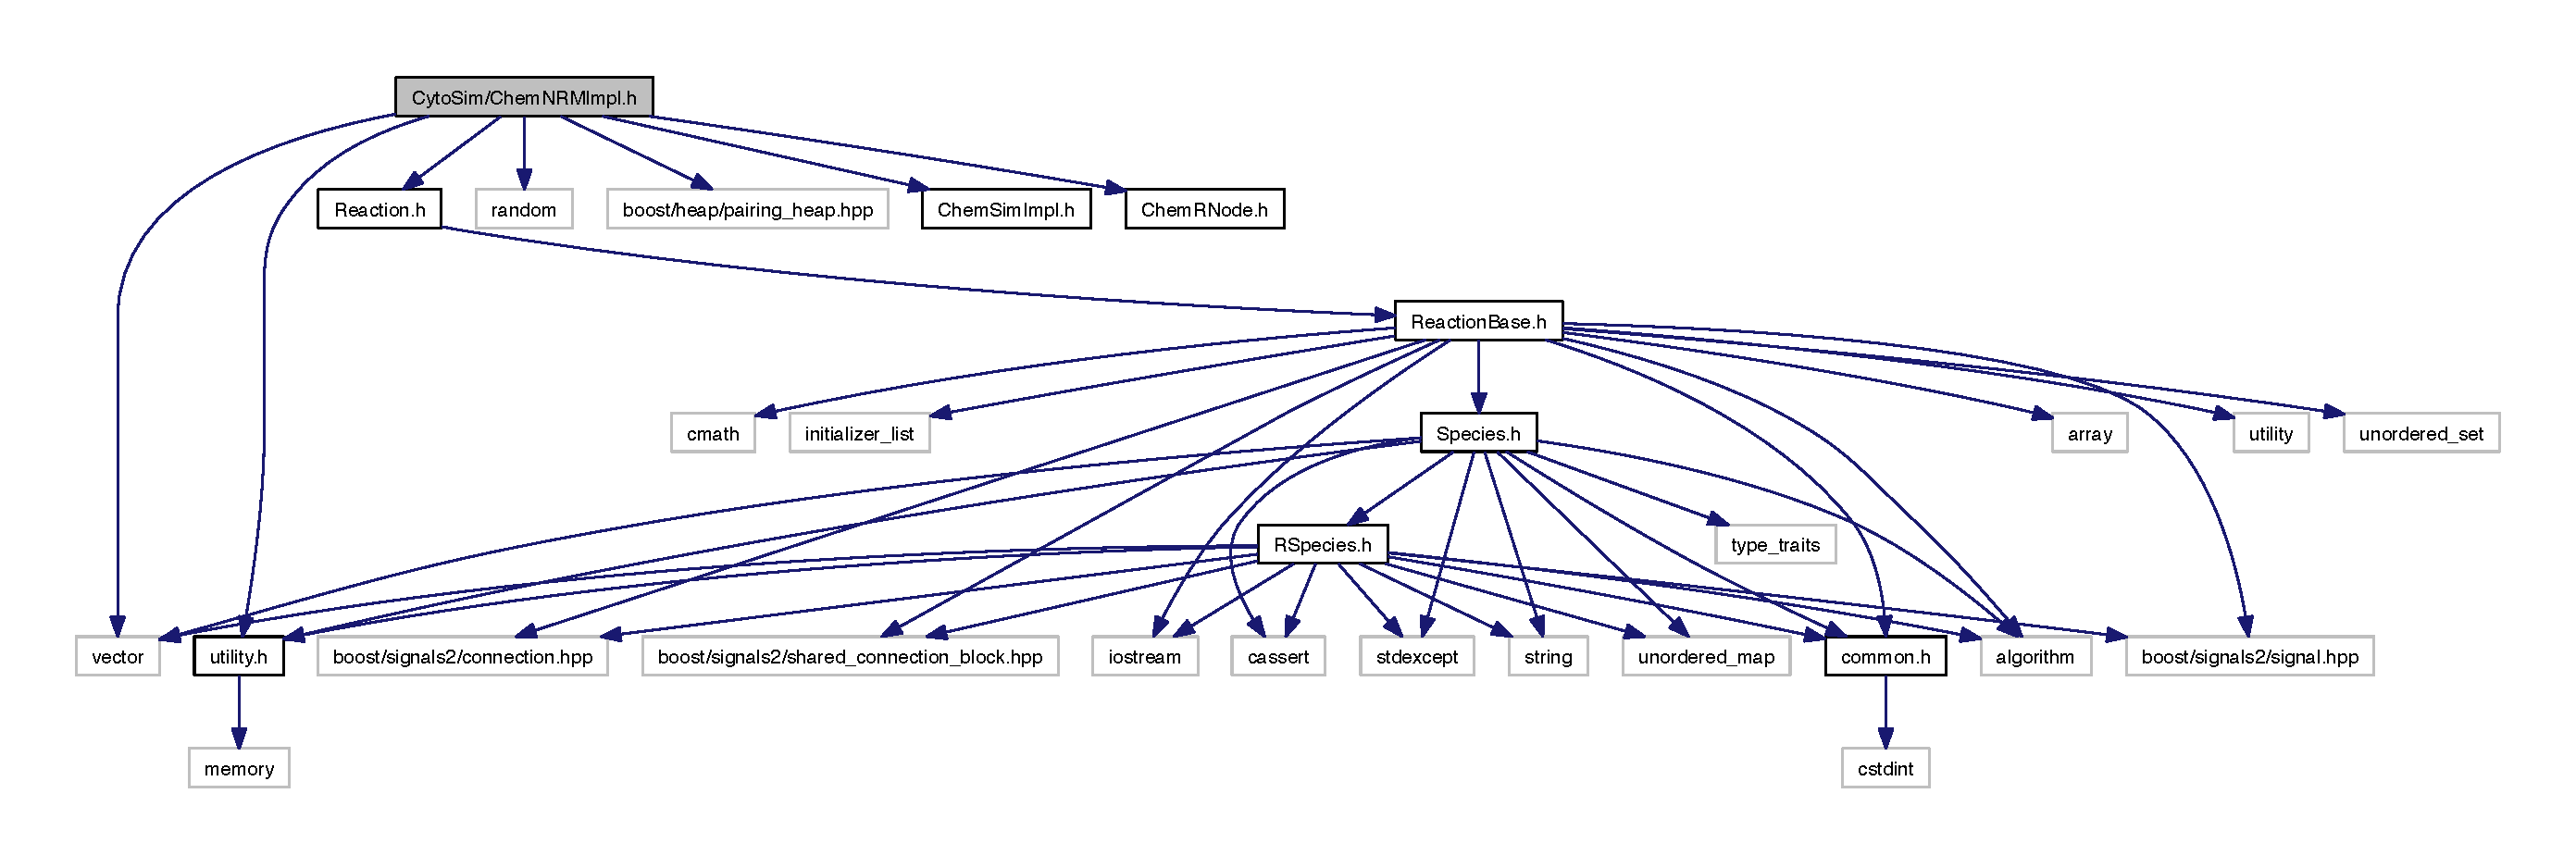
\includegraphics[width=350pt]{ChemNRMImpl_8h__incl}
\end{center}
\end{figure}
This graph shows which files directly or indirectly include this file\+:\nopagebreak
\begin{figure}[H]
\begin{center}
\leavevmode
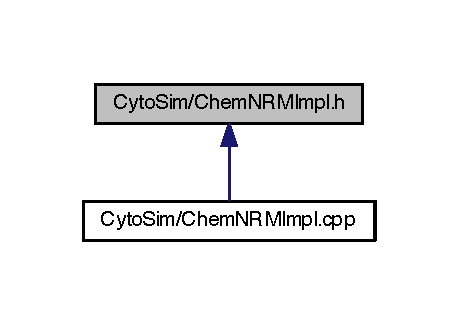
\includegraphics[width=350pt]{ChemNRMImpl_8h__dep__incl}
\end{center}
\end{figure}
\subsection*{Classes}
\begin{DoxyCompactItemize}
\item 
class \hyperlink{classPQNode}{P\+Q\+Node}
\begin{DoxyCompactList}\small\item\em Priority Queue Node. \end{DoxyCompactList}\item 
class \hyperlink{classRNodeNRM}{R\+Node\+N\+R\+M}
\begin{DoxyCompactList}\small\item\em \hyperlink{classReaction}{Reaction} Node for the Next \hyperlink{classReaction}{Reaction} Method. \end{DoxyCompactList}\item 
class \hyperlink{classChemNRMImpl}{Chem\+N\+R\+M\+Impl}
\begin{DoxyCompactList}\small\item\em The chemical Next \hyperlink{classReaction}{Reaction} Method Implementation. \end{DoxyCompactList}\end{DoxyCompactItemize}
\subsection*{Macros}
\begin{DoxyCompactItemize}
\item 
\#define \hyperlink{ChemNRMImpl_8h_ac7284cce00b645fa49b08ae6aecbdc11}{B\+O\+O\+S\+T\+\_\+\+P\+O\+O\+L\+\_\+\+M\+E\+M\+\_\+\+P\+Q\+N\+O\+D\+E}
\begin{DoxyCompactList}\small\item\em The algorithm implemented here is based on the following reference\+: $\ast$$\ast$ Michael A. Gibson, and Jehoshua Bruck J. Phys. Chem. A, 2000, 104 (9), 1876-\/1889 $\ast$$\ast$. \end{DoxyCompactList}\item 
\#define \hyperlink{ChemNRMImpl_8h_a6d805cd02e3606f51cda9faca85b1670}{B\+O\+O\+S\+T\+\_\+\+P\+O\+O\+L\+\_\+\+M\+E\+M\+\_\+\+R\+N\+O\+D\+E\+N\+R\+M}
\item 
\#define \hyperlink{ChemNRMImpl_8h_ad9d458cf298e6ecf4f6b58527b9e5281}{B\+O\+O\+S\+T\+\_\+\+P\+O\+O\+L\+\_\+\+M\+E\+M\+\_\+\+H\+E\+A\+P\+\_\+\+E\+L\+E\+M\+E\+N\+T}
\end{DoxyCompactItemize}
\subsection*{Typedefs}
\begin{DoxyCompactItemize}
\item 
typedef \\*
boost\+::heap\+::pairing\+\_\+heap\\*
$<$ \hyperlink{classPQNode}{P\+Q\+Node} $>$ \hyperlink{ChemNRMImpl_8h_a57f859851909ca786c37681af9b01d45}{boost\+\_\+heap}
\item 
typedef \\*
boost\+::heap\+::pairing\+\_\+heap\\*
$<$ \hyperlink{classPQNode}{P\+Q\+Node} $>$\+::handle\+\_\+type \hyperlink{ChemNRMImpl_8h_a386f0f8003798d7e30dc670c31be1992}{handle\+\_\+t}
\end{DoxyCompactItemize}


\subsection{Macro Definition Documentation}
\hypertarget{ChemNRMImpl_8h_ad9d458cf298e6ecf4f6b58527b9e5281}{\index{Chem\+N\+R\+M\+Impl.\+h@{Chem\+N\+R\+M\+Impl.\+h}!B\+O\+O\+S\+T\+\_\+\+P\+O\+O\+L\+\_\+\+M\+E\+M\+\_\+\+H\+E\+A\+P\+\_\+\+E\+L\+E\+M\+E\+N\+T@{B\+O\+O\+S\+T\+\_\+\+P\+O\+O\+L\+\_\+\+M\+E\+M\+\_\+\+H\+E\+A\+P\+\_\+\+E\+L\+E\+M\+E\+N\+T}}
\index{B\+O\+O\+S\+T\+\_\+\+P\+O\+O\+L\+\_\+\+M\+E\+M\+\_\+\+H\+E\+A\+P\+\_\+\+E\+L\+E\+M\+E\+N\+T@{B\+O\+O\+S\+T\+\_\+\+P\+O\+O\+L\+\_\+\+M\+E\+M\+\_\+\+H\+E\+A\+P\+\_\+\+E\+L\+E\+M\+E\+N\+T}!Chem\+N\+R\+M\+Impl.\+h@{Chem\+N\+R\+M\+Impl.\+h}}
\subsubsection[{B\+O\+O\+S\+T\+\_\+\+P\+O\+O\+L\+\_\+\+M\+E\+M\+\_\+\+H\+E\+A\+P\+\_\+\+E\+L\+E\+M\+E\+N\+T}]{\setlength{\rightskip}{0pt plus 5cm}\#define B\+O\+O\+S\+T\+\_\+\+P\+O\+O\+L\+\_\+\+M\+E\+M\+\_\+\+H\+E\+A\+P\+\_\+\+E\+L\+E\+M\+E\+N\+T}}\label{ChemNRMImpl_8h_ad9d458cf298e6ecf4f6b58527b9e5281}


Definition at line 39 of file Chem\+N\+R\+M\+Impl.\+h.

\hypertarget{ChemNRMImpl_8h_ac7284cce00b645fa49b08ae6aecbdc11}{\index{Chem\+N\+R\+M\+Impl.\+h@{Chem\+N\+R\+M\+Impl.\+h}!B\+O\+O\+S\+T\+\_\+\+P\+O\+O\+L\+\_\+\+M\+E\+M\+\_\+\+P\+Q\+N\+O\+D\+E@{B\+O\+O\+S\+T\+\_\+\+P\+O\+O\+L\+\_\+\+M\+E\+M\+\_\+\+P\+Q\+N\+O\+D\+E}}
\index{B\+O\+O\+S\+T\+\_\+\+P\+O\+O\+L\+\_\+\+M\+E\+M\+\_\+\+P\+Q\+N\+O\+D\+E@{B\+O\+O\+S\+T\+\_\+\+P\+O\+O\+L\+\_\+\+M\+E\+M\+\_\+\+P\+Q\+N\+O\+D\+E}!Chem\+N\+R\+M\+Impl.\+h@{Chem\+N\+R\+M\+Impl.\+h}}
\subsubsection[{B\+O\+O\+S\+T\+\_\+\+P\+O\+O\+L\+\_\+\+M\+E\+M\+\_\+\+P\+Q\+N\+O\+D\+E}]{\setlength{\rightskip}{0pt plus 5cm}\#define B\+O\+O\+S\+T\+\_\+\+P\+O\+O\+L\+\_\+\+M\+E\+M\+\_\+\+P\+Q\+N\+O\+D\+E}}\label{ChemNRMImpl_8h_ac7284cce00b645fa49b08ae6aecbdc11}


The algorithm implemented here is based on the following reference\+: $\ast$$\ast$ Michael A. Gibson, and Jehoshua Bruck J. Phys. Chem. A, 2000, 104 (9), 1876-\/1889 $\ast$$\ast$. 



Definition at line 37 of file Chem\+N\+R\+M\+Impl.\+h.

\hypertarget{ChemNRMImpl_8h_a6d805cd02e3606f51cda9faca85b1670}{\index{Chem\+N\+R\+M\+Impl.\+h@{Chem\+N\+R\+M\+Impl.\+h}!B\+O\+O\+S\+T\+\_\+\+P\+O\+O\+L\+\_\+\+M\+E\+M\+\_\+\+R\+N\+O\+D\+E\+N\+R\+M@{B\+O\+O\+S\+T\+\_\+\+P\+O\+O\+L\+\_\+\+M\+E\+M\+\_\+\+R\+N\+O\+D\+E\+N\+R\+M}}
\index{B\+O\+O\+S\+T\+\_\+\+P\+O\+O\+L\+\_\+\+M\+E\+M\+\_\+\+R\+N\+O\+D\+E\+N\+R\+M@{B\+O\+O\+S\+T\+\_\+\+P\+O\+O\+L\+\_\+\+M\+E\+M\+\_\+\+R\+N\+O\+D\+E\+N\+R\+M}!Chem\+N\+R\+M\+Impl.\+h@{Chem\+N\+R\+M\+Impl.\+h}}
\subsubsection[{B\+O\+O\+S\+T\+\_\+\+P\+O\+O\+L\+\_\+\+M\+E\+M\+\_\+\+R\+N\+O\+D\+E\+N\+R\+M}]{\setlength{\rightskip}{0pt plus 5cm}\#define B\+O\+O\+S\+T\+\_\+\+P\+O\+O\+L\+\_\+\+M\+E\+M\+\_\+\+R\+N\+O\+D\+E\+N\+R\+M}}\label{ChemNRMImpl_8h_a6d805cd02e3606f51cda9faca85b1670}


Definition at line 38 of file Chem\+N\+R\+M\+Impl.\+h.



\subsection{Typedef Documentation}
\hypertarget{ChemNRMImpl_8h_a57f859851909ca786c37681af9b01d45}{\index{Chem\+N\+R\+M\+Impl.\+h@{Chem\+N\+R\+M\+Impl.\+h}!boost\+\_\+heap@{boost\+\_\+heap}}
\index{boost\+\_\+heap@{boost\+\_\+heap}!Chem\+N\+R\+M\+Impl.\+h@{Chem\+N\+R\+M\+Impl.\+h}}
\subsubsection[{boost\+\_\+heap}]{\setlength{\rightskip}{0pt plus 5cm}typedef boost\+::heap\+::pairing\+\_\+heap$<${\bf P\+Q\+Node}$>$ {\bf boost\+\_\+heap}}}\label{ChemNRMImpl_8h_a57f859851909ca786c37681af9b01d45}


Definition at line 44 of file Chem\+N\+R\+M\+Impl.\+h.

\hypertarget{ChemNRMImpl_8h_a386f0f8003798d7e30dc670c31be1992}{\index{Chem\+N\+R\+M\+Impl.\+h@{Chem\+N\+R\+M\+Impl.\+h}!handle\+\_\+t@{handle\+\_\+t}}
\index{handle\+\_\+t@{handle\+\_\+t}!Chem\+N\+R\+M\+Impl.\+h@{Chem\+N\+R\+M\+Impl.\+h}}
\subsubsection[{handle\+\_\+t}]{\setlength{\rightskip}{0pt plus 5cm}typedef boost\+::heap\+::pairing\+\_\+heap$<${\bf P\+Q\+Node}$>$\+::handle\+\_\+type {\bf handle\+\_\+t}}}\label{ChemNRMImpl_8h_a386f0f8003798d7e30dc670c31be1992}


Definition at line 52 of file Chem\+N\+R\+M\+Impl.\+h.


\hypertarget{ChemRNode_8h}{\section{Cyto\-Sim/\-Chem\-R\-Node.h File Reference}
\label{ChemRNode_8h}\index{Cyto\-Sim/\-Chem\-R\-Node.\-h@{Cyto\-Sim/\-Chem\-R\-Node.\-h}}
}
This graph shows which files directly or indirectly include this file\-:\nopagebreak
\begin{figure}[H]
\begin{center}
\leavevmode
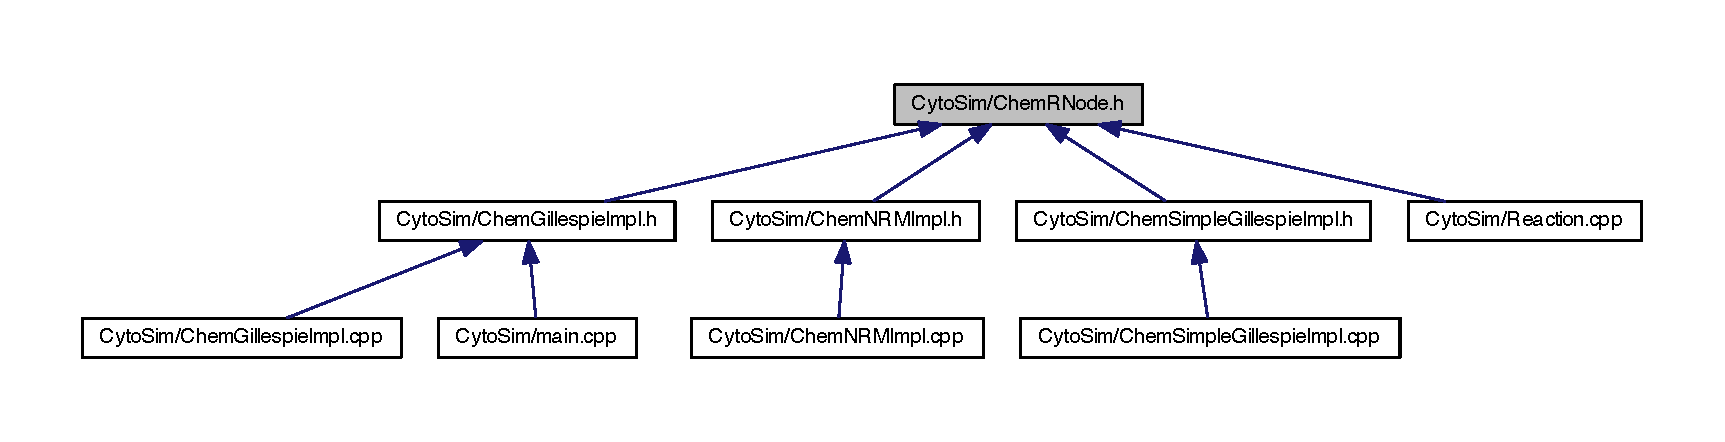
\includegraphics[width=350pt]{ChemRNode_8h__dep__incl}
\end{center}
\end{figure}
\subsection*{Classes}
\begin{DoxyCompactItemize}
\item 
class \hyperlink{classchem_1_1RNode}{chem\-::\-R\-Node}
\begin{DoxyCompactList}\small\item\em This is an abstract base class for classes that need to be associated with the given \hyperlink{classchem_1_1Reaction}{Reaction} object. \end{DoxyCompactList}\end{DoxyCompactItemize}
\subsection*{Namespaces}
\begin{DoxyCompactItemize}
\item 
namespace \hyperlink{namespacechem}{chem}
\end{DoxyCompactItemize}

\hypertarget{ChemSim_8cpp}{\section{Cyto\-Sim/\-Chem\-Sim.cpp File Reference}
\label{ChemSim_8cpp}\index{Cyto\-Sim/\-Chem\-Sim.\-cpp@{Cyto\-Sim/\-Chem\-Sim.\-cpp}}
}
{\ttfamily \#include $<$iostream$>$}\\*
{\ttfamily \#include \char`\"{}Chem\-Sim.\-h\char`\"{}}\\*
{\ttfamily \#include \char`\"{}Chem\-Sim\-Impl.\-h\char`\"{}}\\*
{\ttfamily \#include \char`\"{}utility.\-h\char`\"{}}\\*
Include dependency graph for Chem\-Sim.\-cpp\-:
\nopagebreak
\begin{figure}[H]
\begin{center}
\leavevmode
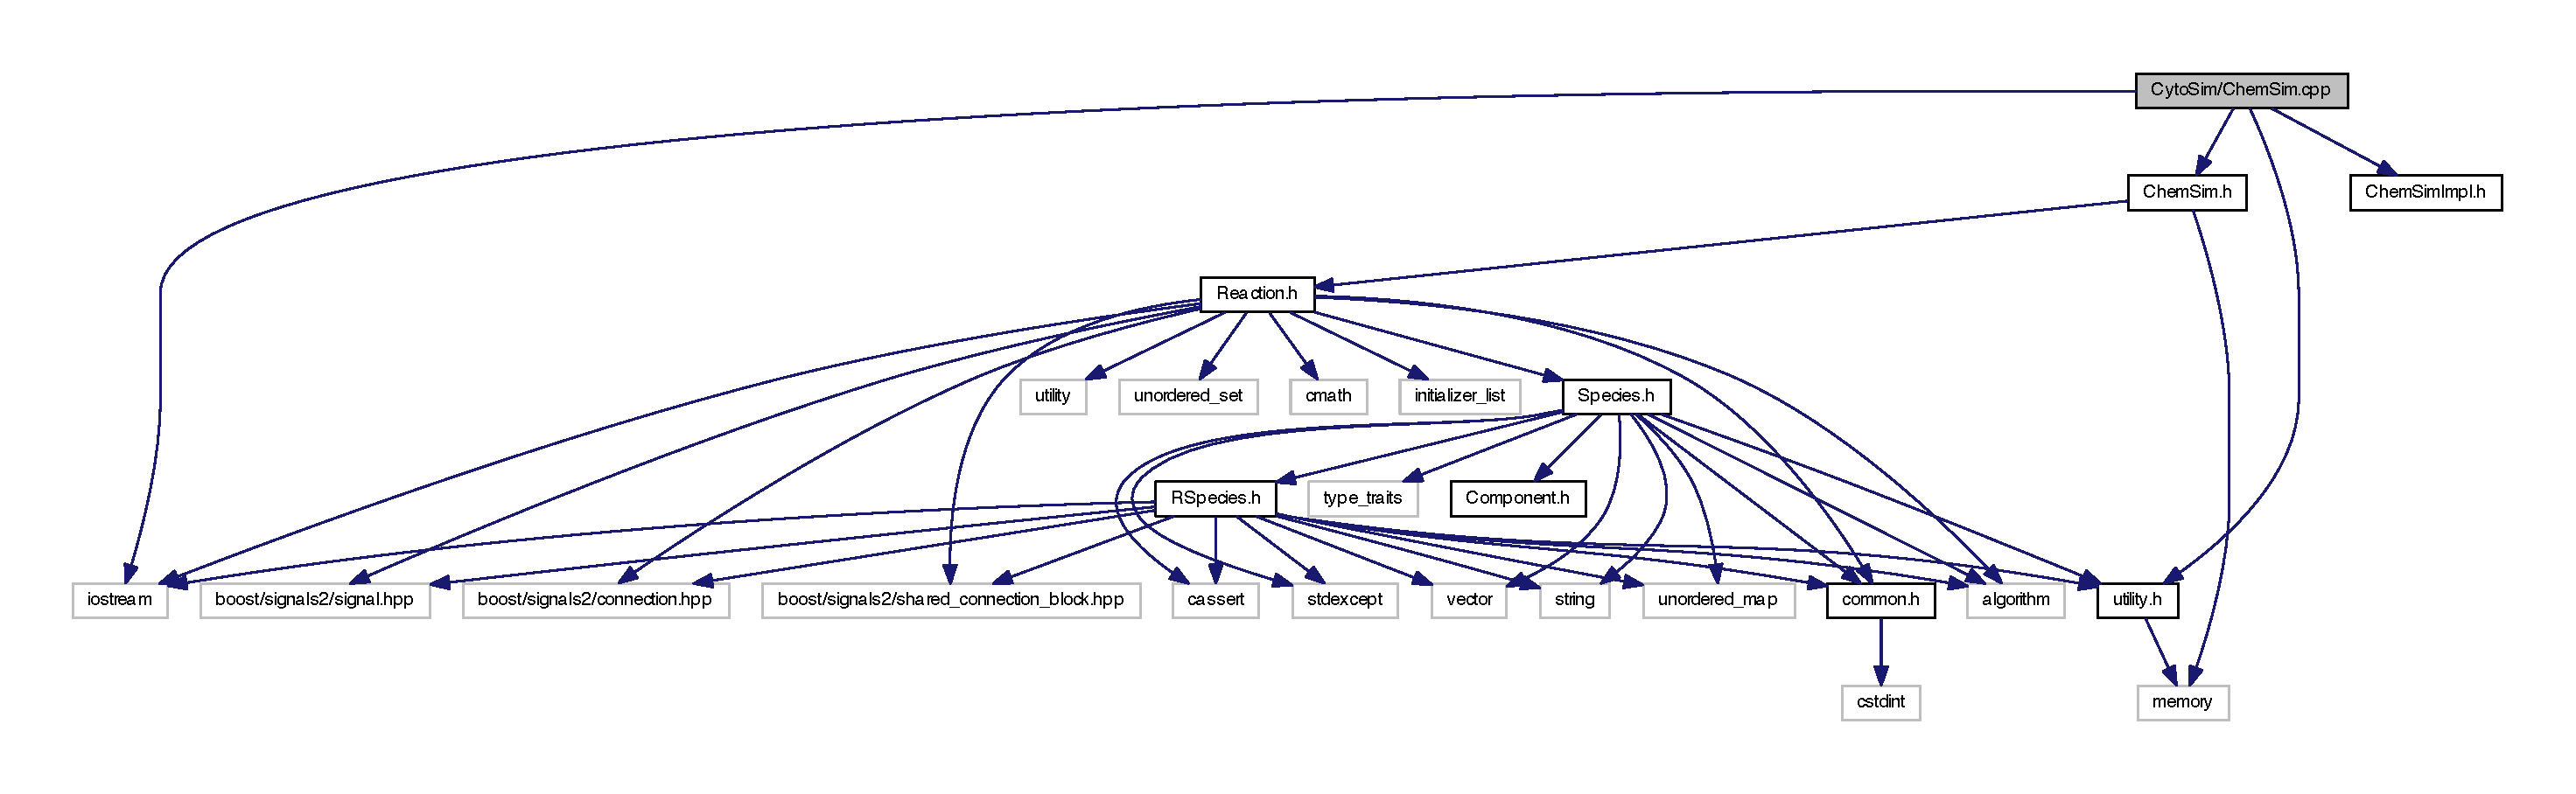
\includegraphics[width=350pt]{ChemSim_8cpp__incl}
\end{center}
\end{figure}
\subsection*{Namespaces}
\begin{DoxyCompactItemize}
\item 
namespace \hyperlink{namespacechem}{chem}
\end{DoxyCompactItemize}

\hypertarget{ChemSim_8h}{\section{Cyto\-Sim/\-Chem\-Sim.h File Reference}
\label{ChemSim_8h}\index{Cyto\-Sim/\-Chem\-Sim.\-h@{Cyto\-Sim/\-Chem\-Sim.\-h}}
}
{\ttfamily \#include $<$memory$>$}\\*
{\ttfamily \#include \char`\"{}Reaction.\-h\char`\"{}}\\*
Include dependency graph for Chem\-Sim.\-h\-:\nopagebreak
\begin{figure}[H]
\begin{center}
\leavevmode
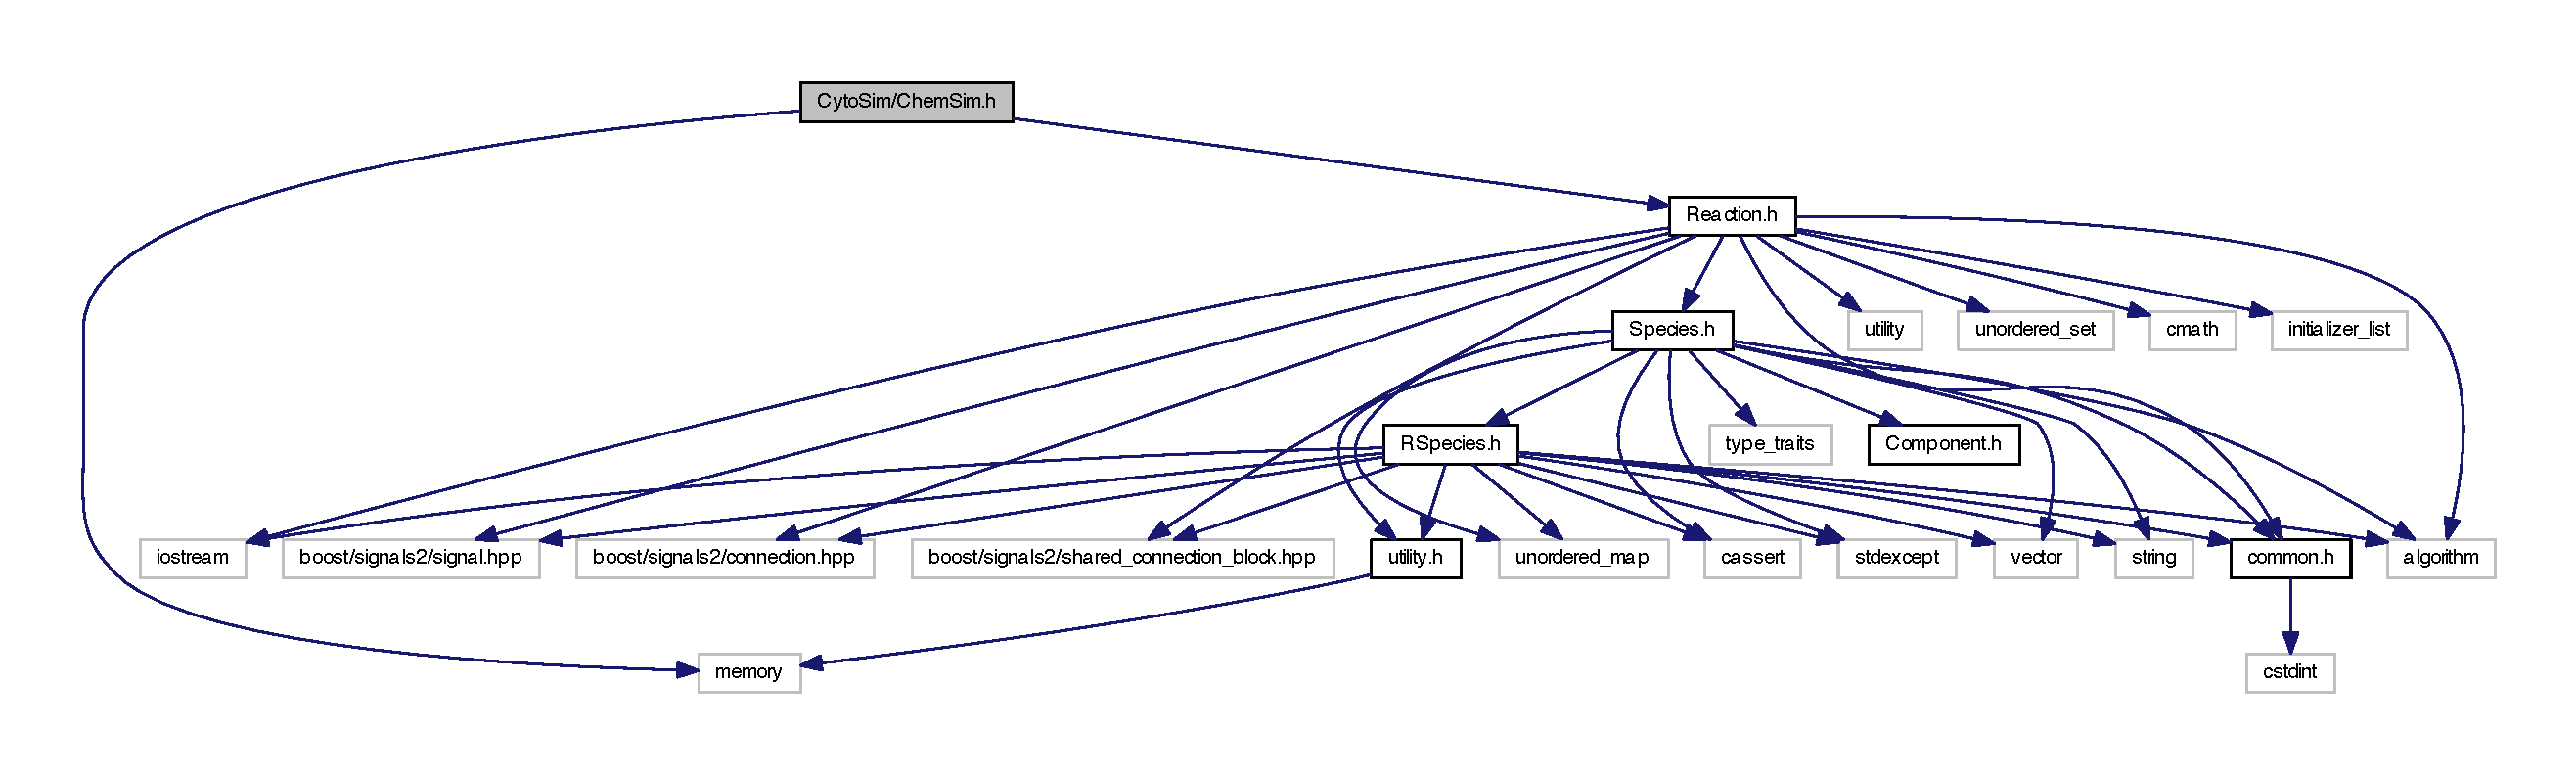
\includegraphics[width=350pt]{ChemSim_8h__incl}
\end{center}
\end{figure}
This graph shows which files directly or indirectly include this file\-:\nopagebreak
\begin{figure}[H]
\begin{center}
\leavevmode
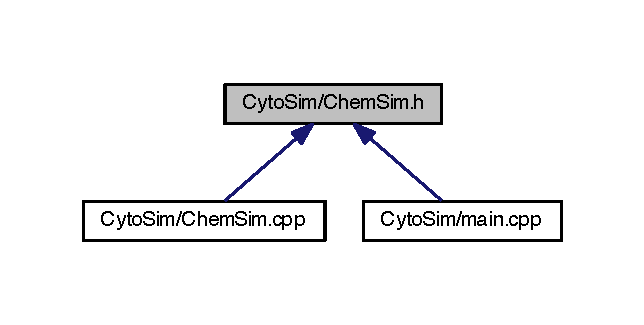
\includegraphics[width=309pt]{ChemSim_8h__dep__incl}
\end{center}
\end{figure}
\subsection*{Classes}
\begin{DoxyCompactItemize}
\item 
class \hyperlink{classchem_1_1ChemSim}{chem\-::\-Chem\-Sim}
\begin{DoxyCompactList}\small\item\em \hyperlink{classchem_1_1ChemSim}{Chem\-Sim} is used to manage running a network of chemical reactions. \end{DoxyCompactList}\end{DoxyCompactItemize}
\subsection*{Namespaces}
\begin{DoxyCompactItemize}
\item 
namespace \hyperlink{namespacechem}{chem}
\begin{DoxyCompactList}\small\item\em The algorithm implemented here is based on the following reference\-: $\ast$$\ast$ Michael A. Gibson, and Jehoshua Bruck J. Phys. Chem. A, 2000, 104 (9), 1876-\/1889 $\ast$$\ast$. \end{DoxyCompactList}\end{DoxyCompactItemize}

\hypertarget{ChemSimImpl_8h}{\section{Cyto\-Sim/\-Chem\-Sim\-Impl.h File Reference}
\label{ChemSimImpl_8h}\index{Cyto\-Sim/\-Chem\-Sim\-Impl.\-h@{Cyto\-Sim/\-Chem\-Sim\-Impl.\-h}}
}
This graph shows which files directly or indirectly include this file\-:\nopagebreak
\begin{figure}[H]
\begin{center}
\leavevmode
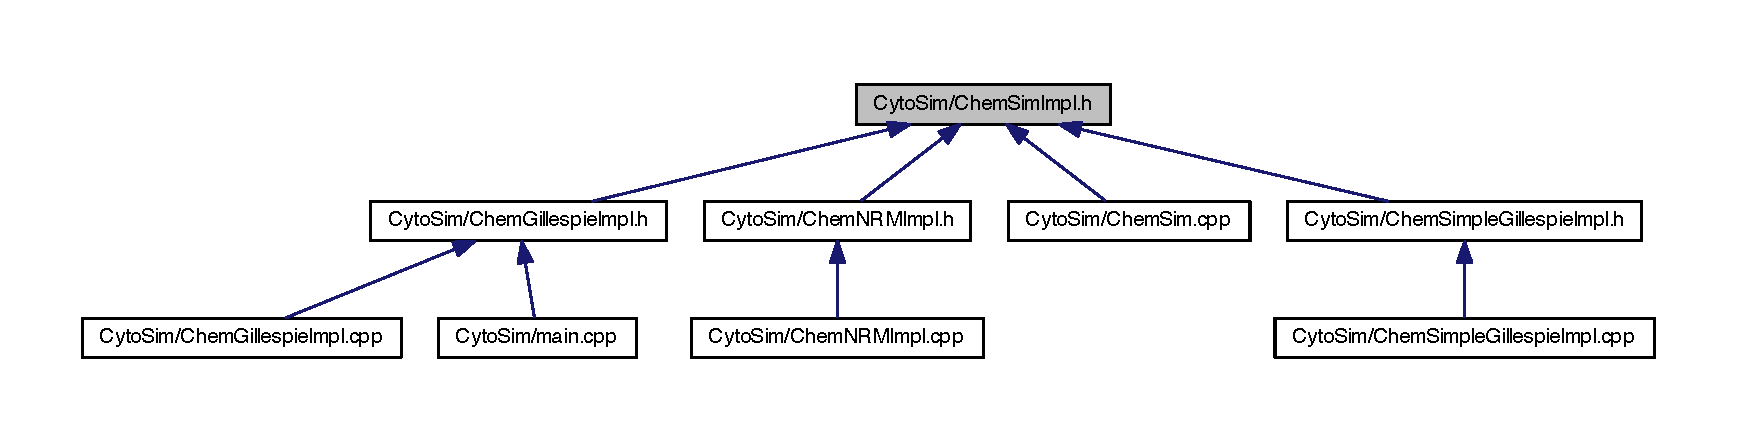
\includegraphics[width=350pt]{ChemSimImpl_8h__dep__incl}
\end{center}
\end{figure}
\subsection*{Classes}
\begin{DoxyCompactItemize}
\item 
class \hyperlink{classchem_1_1ChemSimImpl}{chem\-::\-Chem\-Sim\-Impl}
\begin{DoxyCompactList}\small\item\em \hyperlink{classchem_1_1ChemSimImpl}{Chem\-Sim\-Impl} is an abstract base class for algorithms that run stochastic chemical kinetics. \end{DoxyCompactList}\end{DoxyCompactItemize}
\subsection*{Namespaces}
\begin{DoxyCompactItemize}
\item 
namespace \hyperlink{namespacechem}{chem}
\begin{DoxyCompactList}\small\item\em The algorithm implemented here is based on the following reference\-: $\ast$$\ast$ Michael A. Gibson, and Jehoshua Bruck J. Phys. Chem. A, 2000, 104 (9), 1876-\/1889 $\ast$$\ast$. \end{DoxyCompactList}\end{DoxyCompactItemize}

\hypertarget{ChemSimpleGillespieImpl_8cpp}{\section{M3\+S\+Y\+M/\+Chemistry/\+Chem\+Simple\+Gillespie\+Impl.cpp File Reference}
\label{ChemSimpleGillespieImpl_8cpp}\index{M3\+S\+Y\+M/\+Chemistry/\+Chem\+Simple\+Gillespie\+Impl.\+cpp@{M3\+S\+Y\+M/\+Chemistry/\+Chem\+Simple\+Gillespie\+Impl.\+cpp}}
}
{\ttfamily \#include \char`\"{}Chem\+Simple\+Gillespie\+Impl.\+h\char`\"{}}\\*
Include dependency graph for Chem\+Simple\+Gillespie\+Impl.\+cpp\+:\nopagebreak
\begin{figure}[H]
\begin{center}
\leavevmode
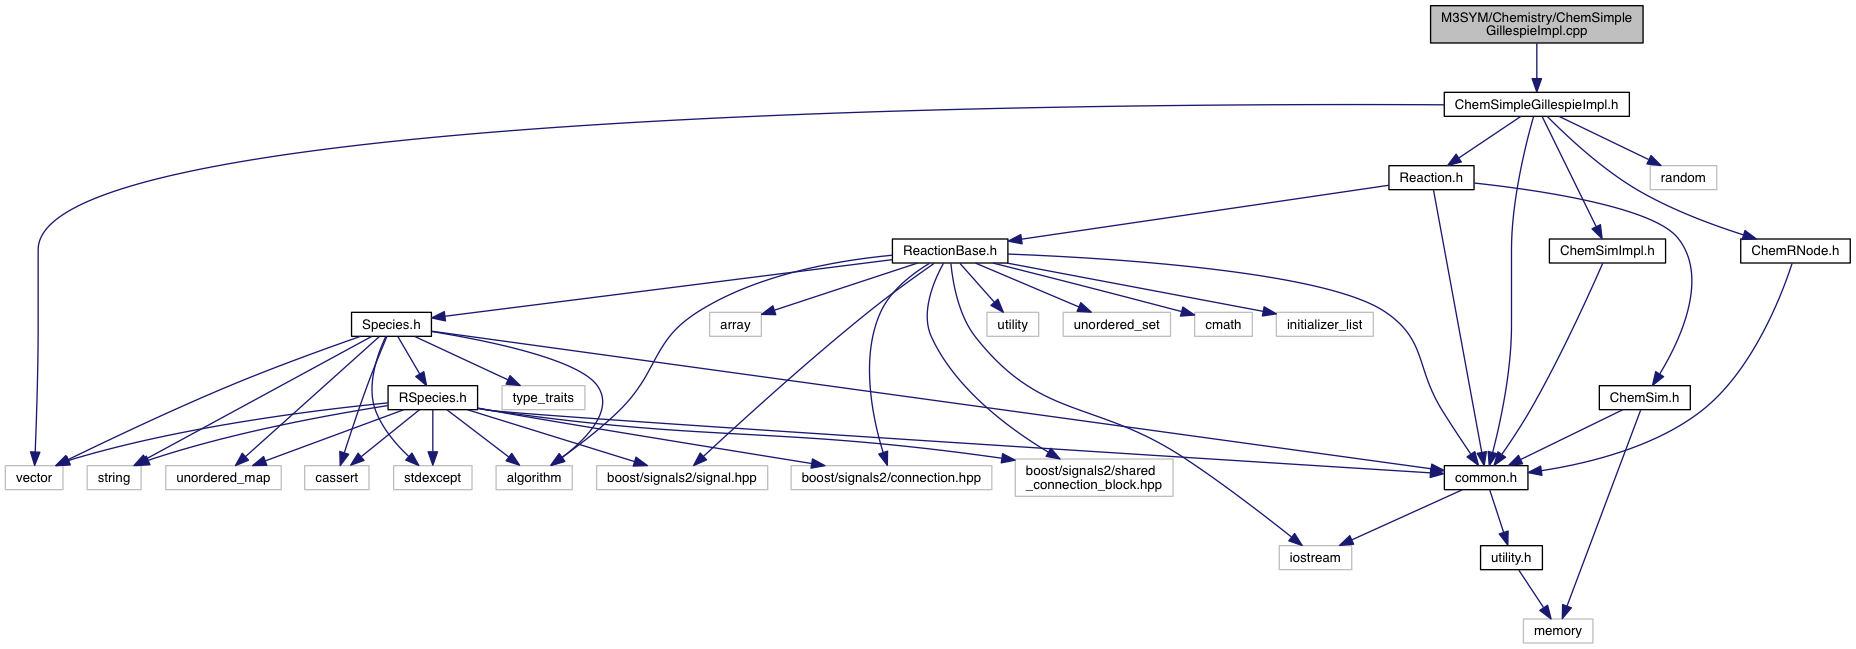
\includegraphics[width=350pt]{ChemSimpleGillespieImpl_8cpp__incl}
\end{center}
\end{figure}

\hypertarget{ChemSimpleGillespieImpl_8h}{\section{M3\+S\+Y\+M/\+Chemistry/\+Chem\+Simple\+Gillespie\+Impl.h File Reference}
\label{ChemSimpleGillespieImpl_8h}\index{M3\+S\+Y\+M/\+Chemistry/\+Chem\+Simple\+Gillespie\+Impl.\+h@{M3\+S\+Y\+M/\+Chemistry/\+Chem\+Simple\+Gillespie\+Impl.\+h}}
}
{\ttfamily \#include $<$vector$>$}\\*
{\ttfamily \#include $<$random$>$}\\*
{\ttfamily \#include \char`\"{}common.\+h\char`\"{}}\\*
{\ttfamily \#include \char`\"{}Reaction.\+h\char`\"{}}\\*
{\ttfamily \#include \char`\"{}Chem\+Sim\+Impl.\+h\char`\"{}}\\*
{\ttfamily \#include \char`\"{}Chem\+R\+Node.\+h\char`\"{}}\\*
Include dependency graph for Chem\+Simple\+Gillespie\+Impl.\+h\+:\nopagebreak
\begin{figure}[H]
\begin{center}
\leavevmode
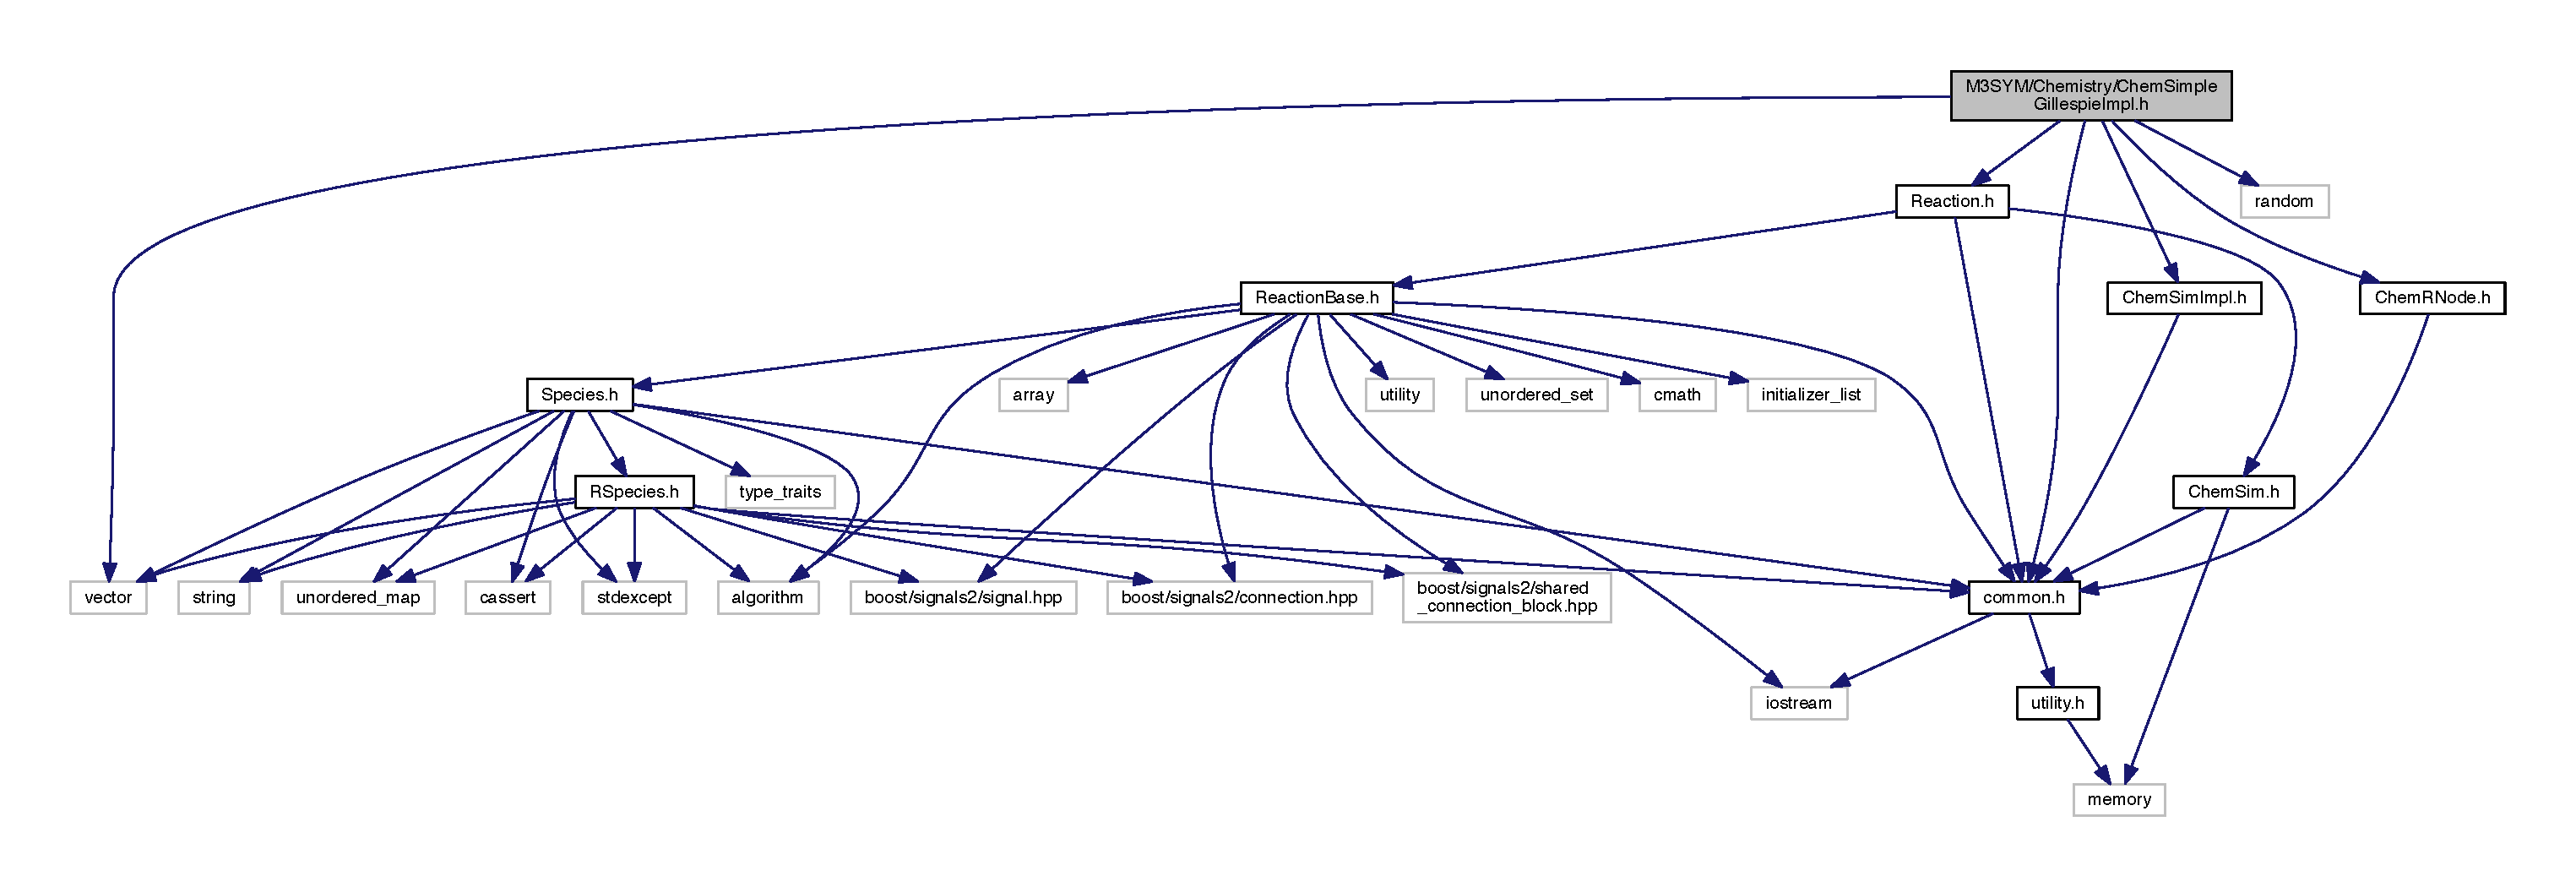
\includegraphics[width=350pt]{ChemSimpleGillespieImpl_8h__incl}
\end{center}
\end{figure}
This graph shows which files directly or indirectly include this file\+:\nopagebreak
\begin{figure}[H]
\begin{center}
\leavevmode
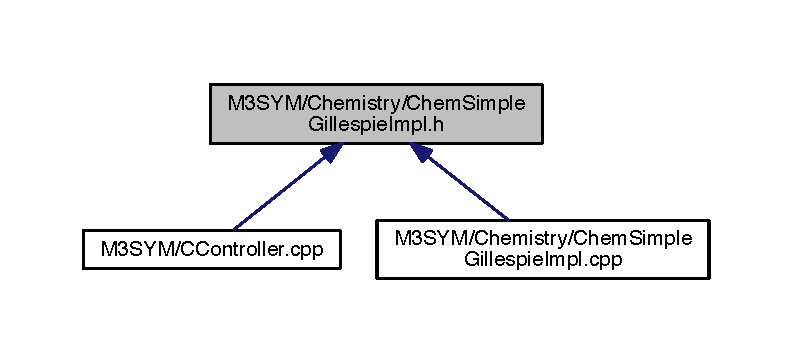
\includegraphics[width=350pt]{ChemSimpleGillespieImpl_8h__dep__incl}
\end{center}
\end{figure}
\subsection*{Classes}
\begin{DoxyCompactItemize}
\item 
class \hyperlink{classChemSimpleGillespieImpl}{Chem\+Simple\+Gillespie\+Impl}
\begin{DoxyCompactList}\small\item\em Implements the simplest version of the Gillespie algorithm, without caching, etc. \end{DoxyCompactList}\end{DoxyCompactItemize}

\hypertarget{common_8cpp}{\section{Cyto\-Sim/common.cpp File Reference}
\label{common_8cpp}\index{Cyto\-Sim/common.\-cpp@{Cyto\-Sim/common.\-cpp}}
}
{\ttfamily \#include $<$iostream$>$}\\*
Include dependency graph for common.\-cpp\-:\nopagebreak
\begin{figure}[H]
\begin{center}
\leavevmode
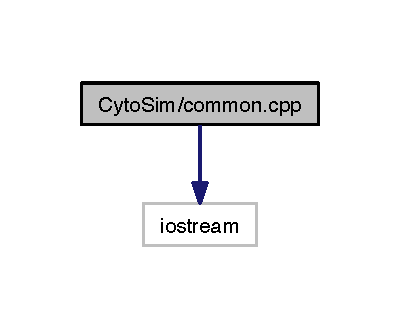
\includegraphics[width=190pt]{common_8cpp__incl}
\end{center}
\end{figure}
\subsection*{Variables}
\begin{DoxyCompactItemize}
\item 
double \hyperlink{common_8cpp_aa3ea98c7e5ad42511b3ec7e0e90e61a4}{global\-\_\-time}
\end{DoxyCompactItemize}


\subsection{Variable Documentation}
\hypertarget{common_8cpp_aa3ea98c7e5ad42511b3ec7e0e90e61a4}{\index{common.\-cpp@{common.\-cpp}!global\-\_\-time@{global\-\_\-time}}
\index{global\-\_\-time@{global\-\_\-time}!common.cpp@{common.\-cpp}}
\subsubsection[{global\-\_\-time}]{\setlength{\rightskip}{0pt plus 5cm}double {\bf global\-\_\-time}}}\label{common_8cpp_aa3ea98c7e5ad42511b3ec7e0e90e61a4}


Definition at line 11 of file common.\-cpp.



Referenced by chem\-::\-Chem\-N\-R\-M\-Impl\-::sync\-Global\-Time(), and tau().


\hypertarget{common_8h}{\section{Cyto\-Sim/common.h File Reference}
\label{common_8h}\index{Cyto\-Sim/common.\-h@{Cyto\-Sim/common.\-h}}
}
{\ttfamily \#include $<$cstdint$>$}\\*
Include dependency graph for common.\-h\-:\nopagebreak
\begin{figure}[H]
\begin{center}
\leavevmode
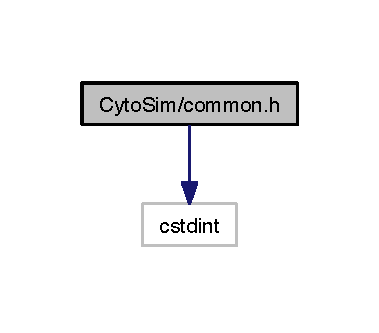
\includegraphics[width=178pt]{common_8h__incl}
\end{center}
\end{figure}
This graph shows which files directly or indirectly include this file\-:\nopagebreak
\begin{figure}[H]
\begin{center}
\leavevmode
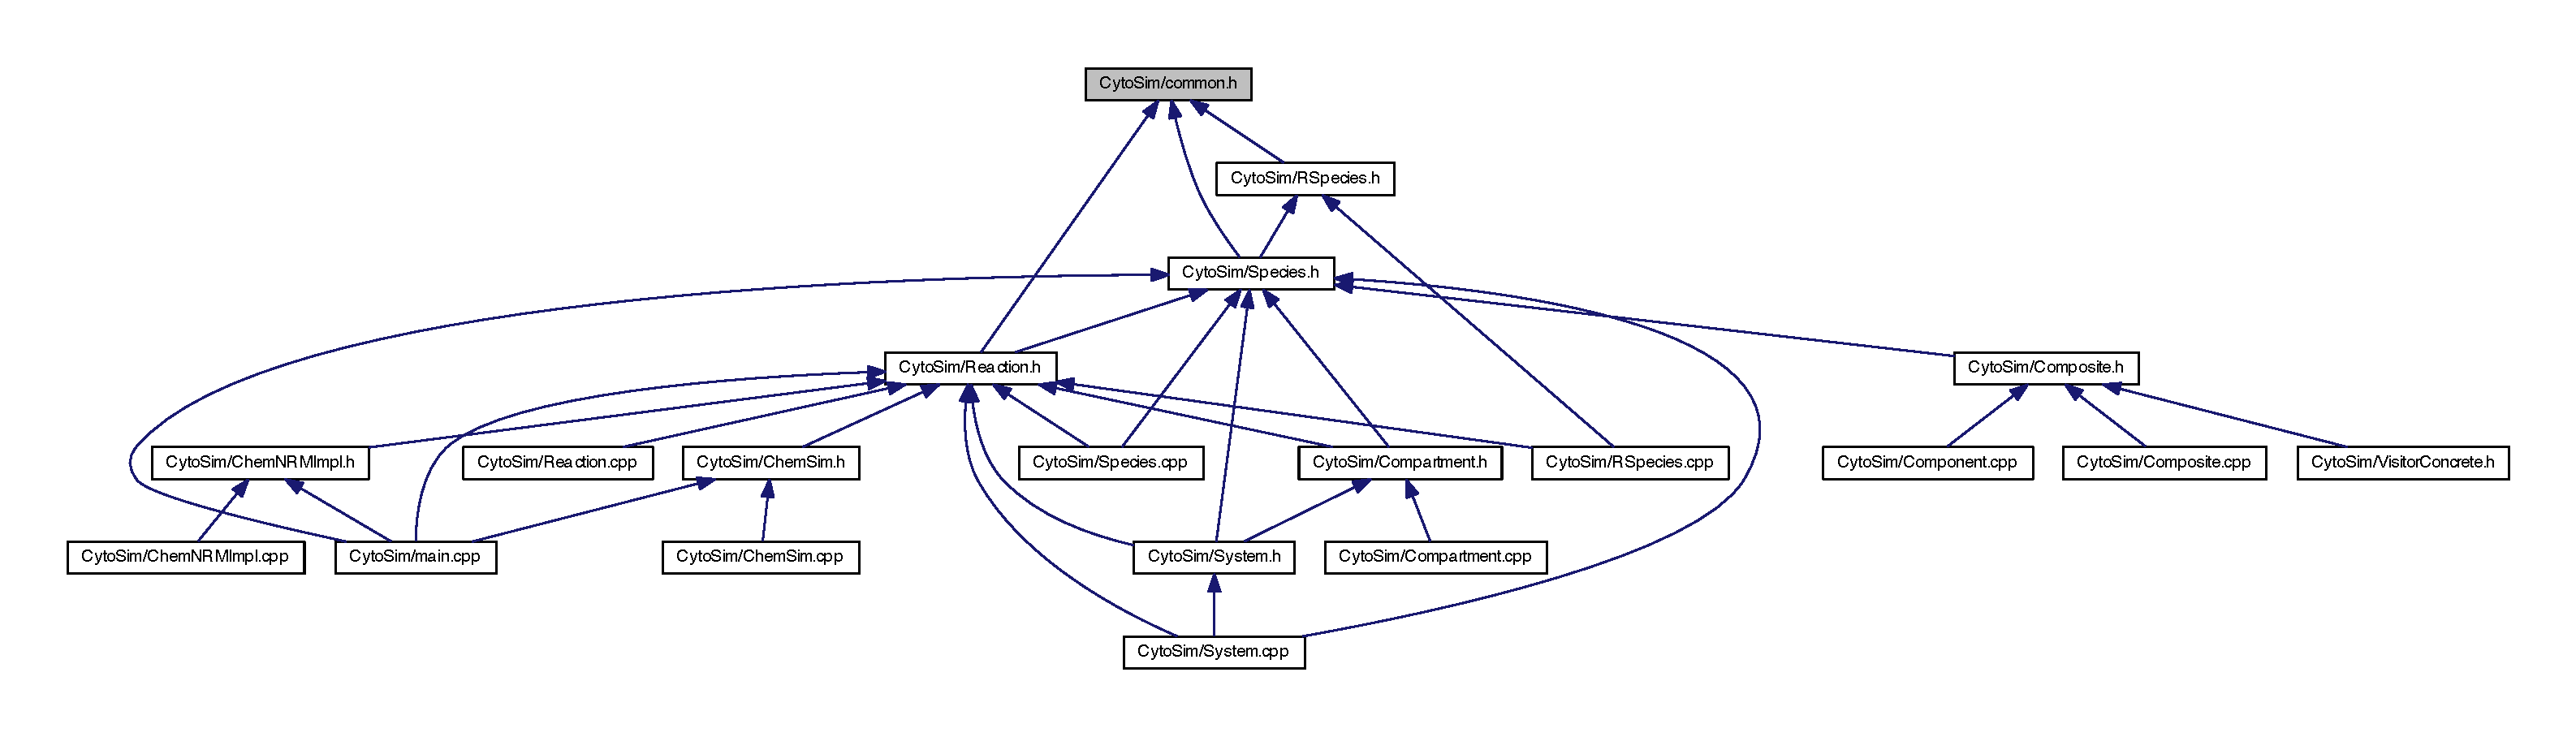
\includegraphics[width=350pt]{common_8h__dep__incl}
\end{center}
\end{figure}
\subsection*{Defines}
\begin{DoxyCompactItemize}
\item 
\#define \hyperlink{common_8h_ac331c2ee4410c5495c7d06314fdbc888}{T\-R\-A\-C\-K\-\_\-\-D\-E\-P\-E\-N\-D\-E\-N\-T\-S}
\item 
\#define \hyperlink{common_8h_a03fd44bcbf25c32054a4982f84f45259}{T\-R\-A\-C\-K\-\_\-\-Z\-E\-R\-O\-\_\-\-C\-O\-P\-Y\-\_\-\-N}
\item 
\#define \hyperlink{common_8h_a318b9661d7fcfe101415b83880576138}{T\-R\-A\-C\-K\-\_\-\-U\-P\-P\-E\-R\-\_\-\-C\-O\-P\-Y\-\_\-\-N}
\end{DoxyCompactItemize}
\subsection*{Typedefs}
\begin{DoxyCompactItemize}
\item 
typedef unsigned short \hyperlink{common_8h_a3503f321fd36304ee274141275cca586}{species\-\_\-copy\-\_\-t}
\end{DoxyCompactItemize}
\subsection*{Functions}
\begin{DoxyCompactItemize}
\item 
double \hyperlink{common_8h_abca55e6a21e0401c42bfb5da79ad3ad5}{tau} ()
\end{DoxyCompactItemize}
\subsection*{Variables}
\begin{DoxyCompactItemize}
\item 
const \hyperlink{common_8h_a3503f321fd36304ee274141275cca586}{species\-\_\-copy\-\_\-t} \hyperlink{common_8h_adaf831a0b61083f29adf8fc6e8edab35}{max\-\_\-ulim} = 1024
\item 
double \hyperlink{common_8h_aa3ea98c7e5ad42511b3ec7e0e90e61a4}{global\-\_\-time}
\end{DoxyCompactItemize}


\subsection{Define Documentation}
\hypertarget{common_8h_ac331c2ee4410c5495c7d06314fdbc888}{\index{common.\-h@{common.\-h}!T\-R\-A\-C\-K\-\_\-\-D\-E\-P\-E\-N\-D\-E\-N\-T\-S@{T\-R\-A\-C\-K\-\_\-\-D\-E\-P\-E\-N\-D\-E\-N\-T\-S}}
\index{T\-R\-A\-C\-K\-\_\-\-D\-E\-P\-E\-N\-D\-E\-N\-T\-S@{T\-R\-A\-C\-K\-\_\-\-D\-E\-P\-E\-N\-D\-E\-N\-T\-S}!common.h@{common.\-h}}
\subsubsection[{T\-R\-A\-C\-K\-\_\-\-D\-E\-P\-E\-N\-D\-E\-N\-T\-S}]{\setlength{\rightskip}{0pt plus 5cm}\#define {\bf T\-R\-A\-C\-K\-\_\-\-D\-E\-P\-E\-N\-D\-E\-N\-T\-S}}}\label{common_8h_ac331c2ee4410c5495c7d06314fdbc888}


Definition at line 12 of file common.\-h.

\hypertarget{common_8h_a318b9661d7fcfe101415b83880576138}{\index{common.\-h@{common.\-h}!T\-R\-A\-C\-K\-\_\-\-U\-P\-P\-E\-R\-\_\-\-C\-O\-P\-Y\-\_\-\-N@{T\-R\-A\-C\-K\-\_\-\-U\-P\-P\-E\-R\-\_\-\-C\-O\-P\-Y\-\_\-\-N}}
\index{T\-R\-A\-C\-K\-\_\-\-U\-P\-P\-E\-R\-\_\-\-C\-O\-P\-Y\-\_\-\-N@{T\-R\-A\-C\-K\-\_\-\-U\-P\-P\-E\-R\-\_\-\-C\-O\-P\-Y\-\_\-\-N}!common.h@{common.\-h}}
\subsubsection[{T\-R\-A\-C\-K\-\_\-\-U\-P\-P\-E\-R\-\_\-\-C\-O\-P\-Y\-\_\-\-N}]{\setlength{\rightskip}{0pt plus 5cm}\#define {\bf T\-R\-A\-C\-K\-\_\-\-U\-P\-P\-E\-R\-\_\-\-C\-O\-P\-Y\-\_\-\-N}}}\label{common_8h_a318b9661d7fcfe101415b83880576138}


Definition at line 14 of file common.\-h.

\hypertarget{common_8h_a03fd44bcbf25c32054a4982f84f45259}{\index{common.\-h@{common.\-h}!T\-R\-A\-C\-K\-\_\-\-Z\-E\-R\-O\-\_\-\-C\-O\-P\-Y\-\_\-\-N@{T\-R\-A\-C\-K\-\_\-\-Z\-E\-R\-O\-\_\-\-C\-O\-P\-Y\-\_\-\-N}}
\index{T\-R\-A\-C\-K\-\_\-\-Z\-E\-R\-O\-\_\-\-C\-O\-P\-Y\-\_\-\-N@{T\-R\-A\-C\-K\-\_\-\-Z\-E\-R\-O\-\_\-\-C\-O\-P\-Y\-\_\-\-N}!common.h@{common.\-h}}
\subsubsection[{T\-R\-A\-C\-K\-\_\-\-Z\-E\-R\-O\-\_\-\-C\-O\-P\-Y\-\_\-\-N}]{\setlength{\rightskip}{0pt plus 5cm}\#define {\bf T\-R\-A\-C\-K\-\_\-\-Z\-E\-R\-O\-\_\-\-C\-O\-P\-Y\-\_\-\-N}}}\label{common_8h_a03fd44bcbf25c32054a4982f84f45259}


Definition at line 13 of file common.\-h.



\subsection{Typedef Documentation}
\hypertarget{common_8h_a3503f321fd36304ee274141275cca586}{\index{common.\-h@{common.\-h}!species\-\_\-copy\-\_\-t@{species\-\_\-copy\-\_\-t}}
\index{species\-\_\-copy\-\_\-t@{species\-\_\-copy\-\_\-t}!common.h@{common.\-h}}
\subsubsection[{species\-\_\-copy\-\_\-t}]{\setlength{\rightskip}{0pt plus 5cm}typedef unsigned short {\bf species\-\_\-copy\-\_\-t}}}\label{common_8h_a3503f321fd36304ee274141275cca586}


Definition at line 18 of file common.\-h.



\subsection{Function Documentation}
\hypertarget{common_8h_abca55e6a21e0401c42bfb5da79ad3ad5}{\index{common.\-h@{common.\-h}!tau@{tau}}
\index{tau@{tau}!common.h@{common.\-h}}
\subsubsection[{tau}]{\setlength{\rightskip}{0pt plus 5cm}double {\bf tau} (
\begin{DoxyParamCaption}
{}
\end{DoxyParamCaption}
)\hspace{0.3cm}{\ttfamily  \mbox{[}inline\mbox{]}}}}\label{common_8h_abca55e6a21e0401c42bfb5da79ad3ad5}


Definition at line 22 of file common.\-h.



References global\-\_\-time.



Referenced by chem\-::\-R\-Node\-N\-R\-M\-::generate\-New\-Rand\-Tau(), chem\-::\-Chem\-Simple\-Gillespie\-Impl\-::make\-Step(), chem\-::\-Chem\-Gillespie\-Impl\-::make\-Step(), chem\-::\-R\-Node\-N\-R\-M\-::passivate\-Reaction(), and chem\-::\-R\-Node\-N\-R\-M\-::set\-Tau().



\subsection{Variable Documentation}
\hypertarget{common_8h_aa3ea98c7e5ad42511b3ec7e0e90e61a4}{\index{common.\-h@{common.\-h}!global\-\_\-time@{global\-\_\-time}}
\index{global\-\_\-time@{global\-\_\-time}!common.h@{common.\-h}}
\subsubsection[{global\-\_\-time}]{\setlength{\rightskip}{0pt plus 5cm}double {\bf global\-\_\-time}}}\label{common_8h_aa3ea98c7e5ad42511b3ec7e0e90e61a4}


Definition at line 11 of file common.\-cpp.



Referenced by chem\-::\-Chem\-Simple\-Gillespie\-Impl\-::sync\-Global\-Time(), chem\-::\-Chem\-Gillespie\-Impl\-::sync\-Global\-Time(), chem\-::\-Chem\-N\-R\-M\-Impl\-::sync\-Global\-Time(), and tau().

\hypertarget{common_8h_adaf831a0b61083f29adf8fc6e8edab35}{\index{common.\-h@{common.\-h}!max\-\_\-ulim@{max\-\_\-ulim}}
\index{max\-\_\-ulim@{max\-\_\-ulim}!common.h@{common.\-h}}
\subsubsection[{max\-\_\-ulim}]{\setlength{\rightskip}{0pt plus 5cm}const {\bf species\-\_\-copy\-\_\-t} {\bf max\-\_\-ulim} = 1024}}\label{common_8h_adaf831a0b61083f29adf8fc6e8edab35}


Definition at line 19 of file common.\-h.


\hypertarget{Compartment_8cpp}{\section{Cyto\-Sim/\-Compartment.cpp File Reference}
\label{Compartment_8cpp}\index{Cyto\-Sim/\-Compartment.\-cpp@{Cyto\-Sim/\-Compartment.\-cpp}}
}
{\ttfamily \#include \char`\"{}Compartment.\-h\char`\"{}}\\*
{\ttfamily \#include \char`\"{}Visitor.\-h\char`\"{}}\\*
Include dependency graph for Compartment.\-cpp\-:
\nopagebreak
\begin{figure}[H]
\begin{center}
\leavevmode
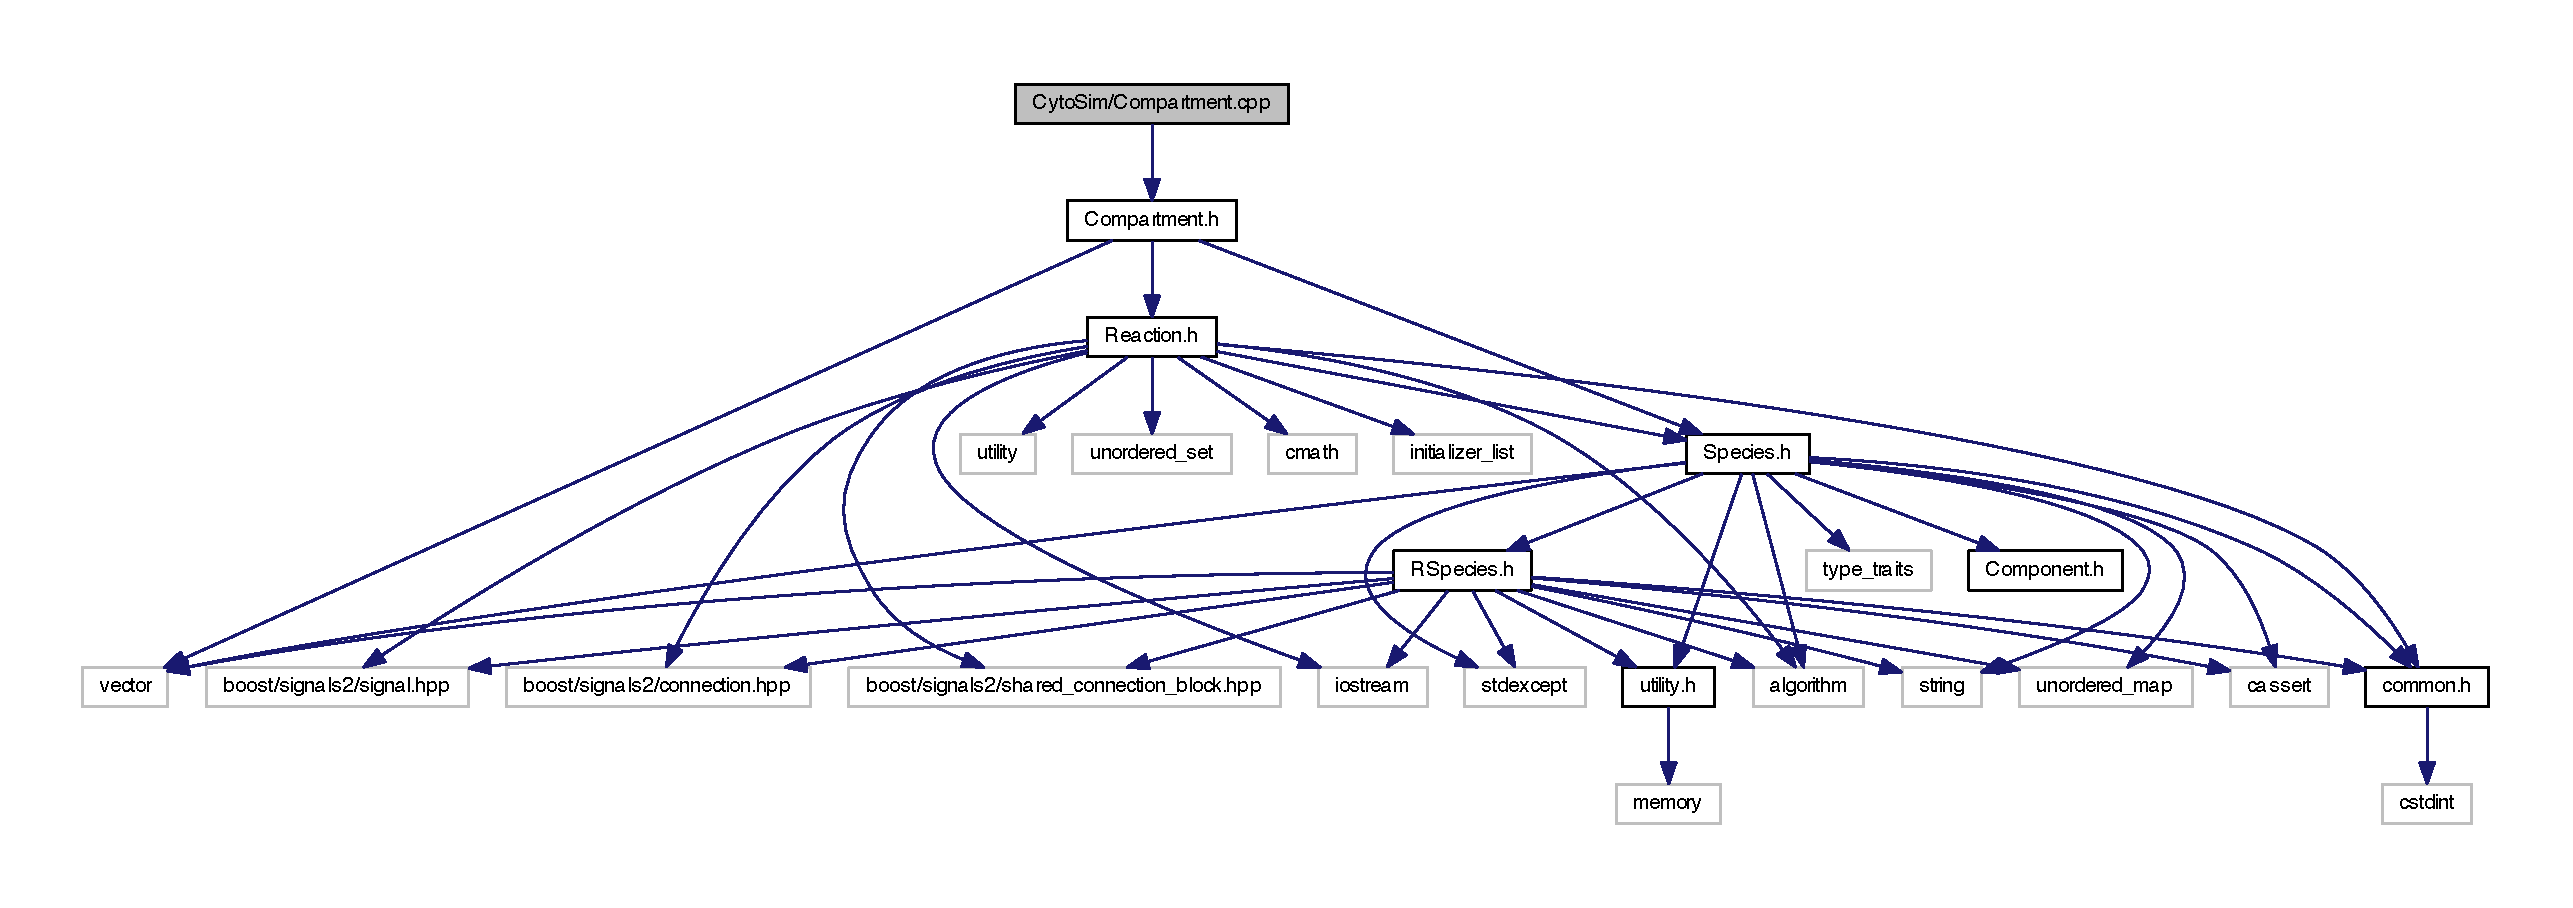
\includegraphics[width=350pt]{Compartment_8cpp__incl}
\end{center}
\end{figure}
\subsection*{Namespaces}
\begin{DoxyCompactItemize}
\item 
namespace \hyperlink{namespacechem}{chem}
\end{DoxyCompactItemize}
\subsection*{Functions}
\begin{DoxyCompactItemize}
\item 
bool \hyperlink{namespacechem_a9342b2280a45cc2043074e2a618be723}{chem\-::operator==} (const Compartment \&a, const Compartment \&b)
\end{DoxyCompactItemize}

\hypertarget{Compartment_8h}{\section{Cyto\-Sim/\-Compartment.h File Reference}
\label{Compartment_8h}\index{Cyto\-Sim/\-Compartment.\-h@{Cyto\-Sim/\-Compartment.\-h}}
}
{\ttfamily \#include $<$vector$>$}\\*
{\ttfamily \#include $<$array$>$}\\*
{\ttfamily \#include $<$unordered\-\_\-map$>$}\\*
{\ttfamily \#include \char`\"{}Reaction.\-h\char`\"{}}\\*
{\ttfamily \#include \char`\"{}Species.\-h\char`\"{}}\\*
{\ttfamily \#include \char`\"{}Species\-Container.\-h\char`\"{}}\\*
{\ttfamily \#include \char`\"{}Reaction\-Container.\-h\char`\"{}}\\*
{\ttfamily \#include \char`\"{}Composite.\-h\char`\"{}}\\*
{\ttfamily \#include \char`\"{}Chem\-Sim.\-h\char`\"{}}\\*
Include dependency graph for Compartment.\-h\-:
\nopagebreak
\begin{figure}[H]
\begin{center}
\leavevmode
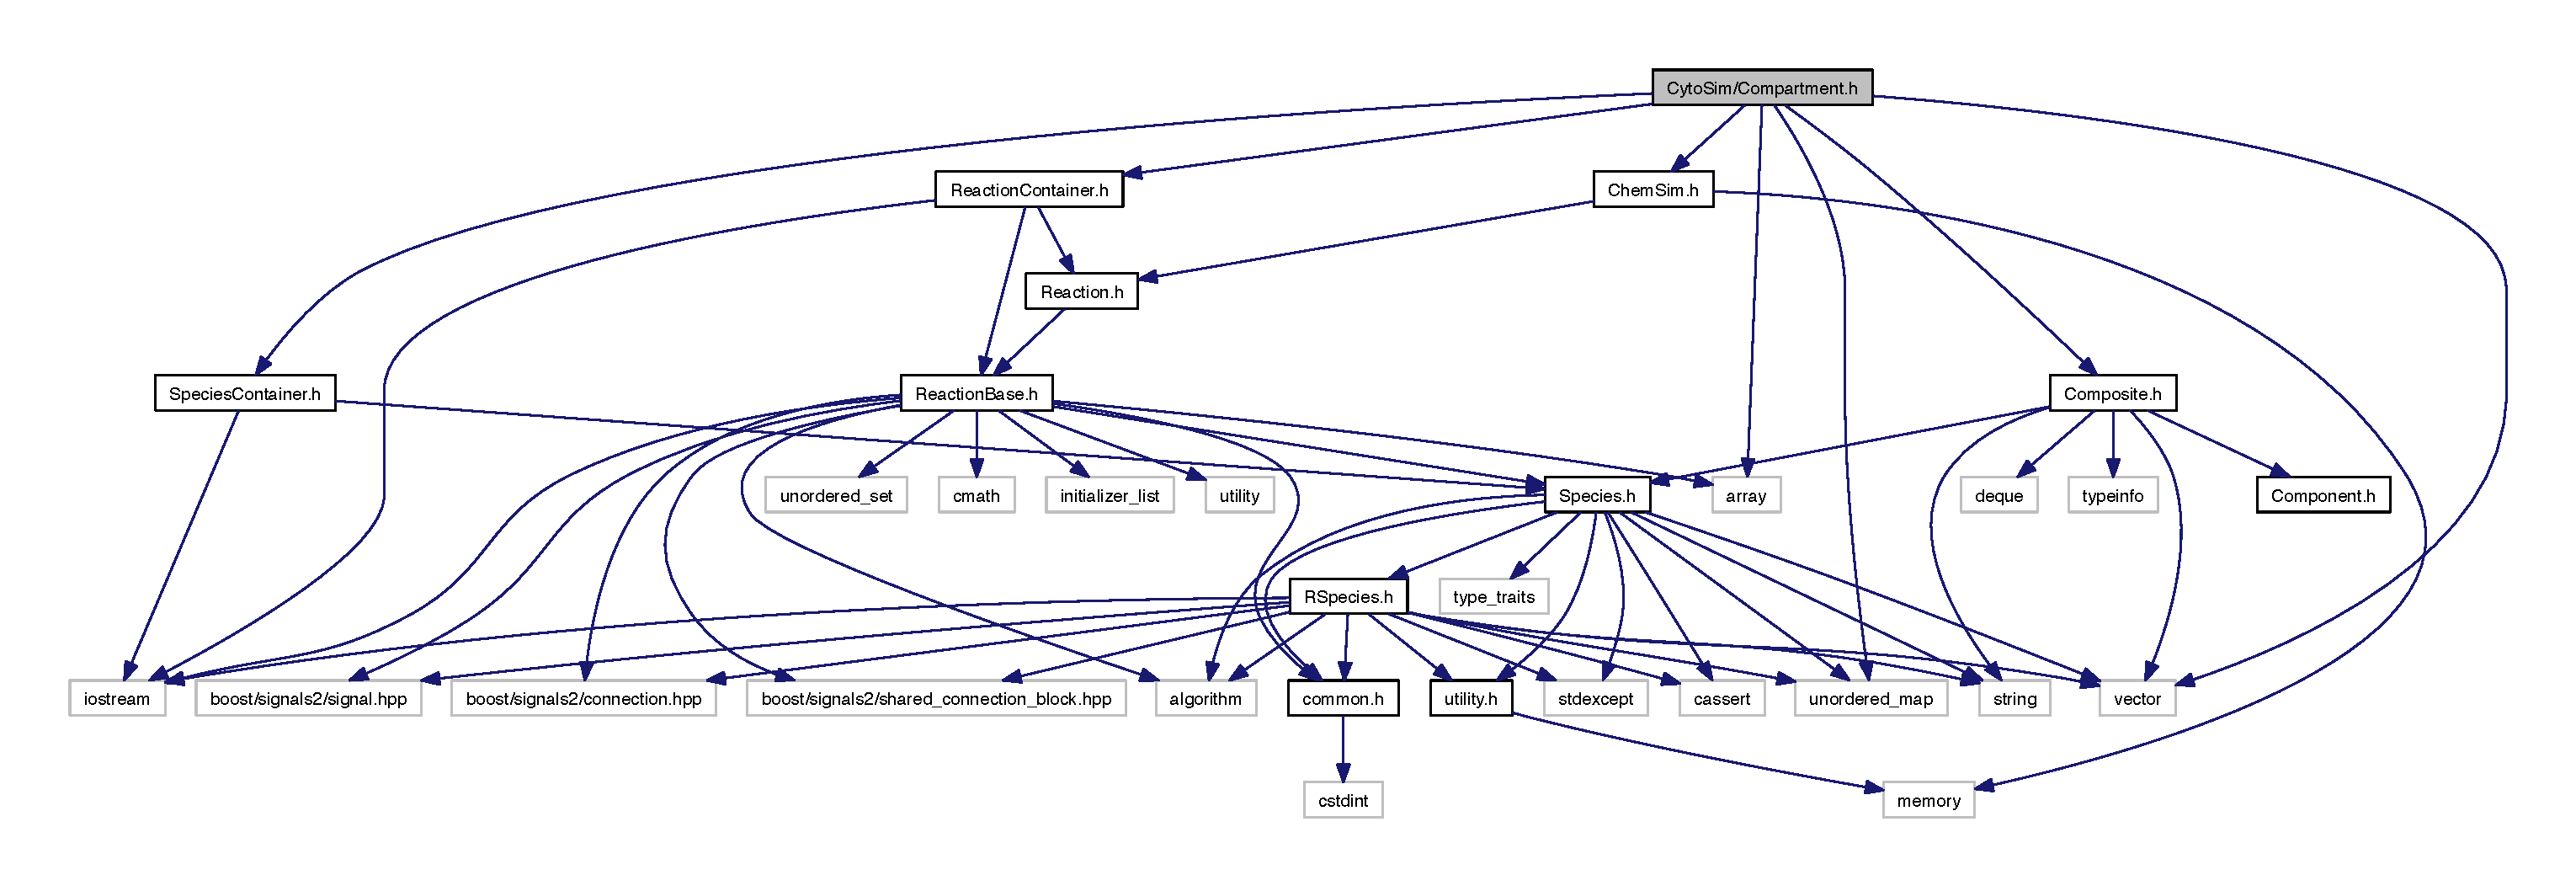
\includegraphics[width=350pt]{Compartment_8h__incl}
\end{center}
\end{figure}
This graph shows which files directly or indirectly include this file\-:
\nopagebreak
\begin{figure}[H]
\begin{center}
\leavevmode
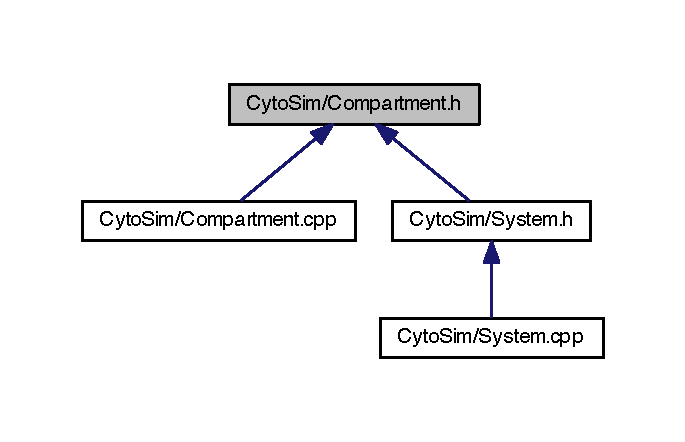
\includegraphics[width=329pt]{Compartment_8h__dep__incl}
\end{center}
\end{figure}
\subsection*{Classes}
\begin{DoxyCompactItemize}
\item 
class \hyperlink{classchem_1_1Compartment}{chem\-::\-Compartment}
\item 
class \hyperlink{classchem_1_1CompartmentCubic}{chem\-::\-Compartment\-Cubic$<$ N\-D\-I\-M $>$}
\end{DoxyCompactItemize}
\subsection*{Namespaces}
\begin{DoxyCompactItemize}
\item 
namespace \hyperlink{namespacechem}{chem}
\end{DoxyCompactItemize}

\hypertarget{CompartmentContainer_8cpp}{\section{M3\+S\+Y\+M/\+Structure/\+Compartment\+Container.cpp File Reference}
\label{CompartmentContainer_8cpp}\index{M3\+S\+Y\+M/\+Structure/\+Compartment\+Container.\+cpp@{M3\+S\+Y\+M/\+Structure/\+Compartment\+Container.\+cpp}}
}
{\ttfamily \#include \char`\"{}Compartment\+Container.\+h\char`\"{}}\\*
Include dependency graph for Compartment\+Container.\+cpp\+:\nopagebreak
\begin{figure}[H]
\begin{center}
\leavevmode
\includegraphics[width=350pt]{CompartmentContainer_8cpp__incl}
\end{center}
\end{figure}

\hypertarget{CompartmentContainer_8h}{\section{M3\+S\+Y\+M/\+Structure/\+Compartment\+Container.h File Reference}
\label{CompartmentContainer_8h}\index{M3\+S\+Y\+M/\+Structure/\+Compartment\+Container.\+h@{M3\+S\+Y\+M/\+Structure/\+Compartment\+Container.\+h}}
}
{\ttfamily \#include \char`\"{}common.\+h\char`\"{}}\\*
{\ttfamily \#include \char`\"{}Compartment.\+h\char`\"{}}\\*
Include dependency graph for Compartment\+Container.\+h\+:\nopagebreak
\begin{figure}[H]
\begin{center}
\leavevmode
\includegraphics[width=350pt]{CompartmentContainer_8h__incl}
\end{center}
\end{figure}
This graph shows which files directly or indirectly include this file\+:\nopagebreak
\begin{figure}[H]
\begin{center}
\leavevmode
\includegraphics[width=350pt]{CompartmentContainer_8h__dep__incl}
\end{center}
\end{figure}
\subsection*{Classes}
\begin{DoxyCompactItemize}
\item 
class \hyperlink{classCompartmentGrid}{Compartment\+Grid}
\begin{DoxyCompactList}\small\item\em A simple n-\/dimensional grid of \hyperlink{classCompartment}{Compartment} objects (singleton). \end{DoxyCompactList}\end{DoxyCompactItemize}

\hypertarget{Component_8cpp}{\section{M3\+S\+Y\+M/\+Component.cpp File Reference}
\label{Component_8cpp}\index{M3\+S\+Y\+M/\+Component.\+cpp@{M3\+S\+Y\+M/\+Component.\+cpp}}
}
{\ttfamily \#include \char`\"{}Component.\+h\char`\"{}}\\*
{\ttfamily \#include \char`\"{}Composite.\+h\char`\"{}}\\*
{\ttfamily \#include \char`\"{}Visitor.\+h\char`\"{}}\\*
Include dependency graph for Component.\+cpp\+:\nopagebreak
\begin{figure}[H]
\begin{center}
\leavevmode
\includegraphics[width=350pt]{Component_8cpp__incl}
\end{center}
\end{figure}

\hypertarget{Component_8h}{\section{Cyto\-Sim/\-Component.h File Reference}
\label{Component_8h}\index{Cyto\-Sim/\-Component.\-h@{Cyto\-Sim/\-Component.\-h}}
}
This graph shows which files directly or indirectly include this file\-:
\nopagebreak
\begin{figure}[H]
\begin{center}
\leavevmode
\includegraphics[width=350pt]{Component_8h__dep__incl}
\end{center}
\end{figure}
\subsection*{Classes}
\begin{DoxyCompactItemize}
\item 
class \hyperlink{classchem_1_1Component}{chem\-::\-Component}
\end{DoxyCompactItemize}
\subsection*{Namespaces}
\begin{DoxyCompactItemize}
\item 
namespace \hyperlink{namespacechem}{chem}
\end{DoxyCompactItemize}

\hypertarget{Composite_8cpp}{\section{Cyto\-Sim/\-Composite.cpp File Reference}
\label{Composite_8cpp}\index{Cyto\-Sim/\-Composite.\-cpp@{Cyto\-Sim/\-Composite.\-cpp}}
}
{\ttfamily \#include $<$iostream$>$}\\*
{\ttfamily \#include \char`\"{}Composite.\-h\char`\"{}}\\*
Include dependency graph for Composite.\-cpp\-:\nopagebreak
\begin{figure}[H]
\begin{center}
\leavevmode
\includegraphics[width=350pt]{Composite_8cpp__incl}
\end{center}
\end{figure}

\hypertarget{Composite_8h}{\section{Cyto\-Sim/\-Composite.h File Reference}
\label{Composite_8h}\index{Cyto\-Sim/\-Composite.\-h@{Cyto\-Sim/\-Composite.\-h}}
}
{\ttfamily \#include $<$string$>$}\\*
{\ttfamily \#include $<$vector$>$}\\*
{\ttfamily \#include $<$deque$>$}\\*
{\ttfamily \#include $<$typeinfo$>$}\\*
{\ttfamily \#include \char`\"{}Component.\-h\char`\"{}}\\*
{\ttfamily \#include \char`\"{}Species.\-h\char`\"{}}\\*
Include dependency graph for Composite.\-h\-:\nopagebreak
\begin{figure}[H]
\begin{center}
\leavevmode
\includegraphics[width=350pt]{Composite_8h__incl}
\end{center}
\end{figure}
This graph shows which files directly or indirectly include this file\-:\nopagebreak
\begin{figure}[H]
\begin{center}
\leavevmode
\includegraphics[width=350pt]{Composite_8h__dep__incl}
\end{center}
\end{figure}
\subsection*{Classes}
\begin{DoxyCompactItemize}
\item 
class \hyperlink{classchem_1_1Composite}{chem\-::\-Composite}
\begin{DoxyCompactList}\small\item\em \hyperlink{classchem_1_1Composite}{Composite} class is the aggregating class for the \hyperlink{classchem_1_1Composite}{Composite} pattern. \end{DoxyCompactList}\end{DoxyCompactItemize}
\subsection*{Namespaces}
\begin{DoxyCompactItemize}
\item 
namespace \hyperlink{namespacechem}{chem}
\end{DoxyCompactItemize}

\hypertarget{main_8cpp}{\section{Cyto\-Sim/main.cpp File Reference}
\label{main_8cpp}\index{Cyto\-Sim/main.\-cpp@{Cyto\-Sim/main.\-cpp}}
}
{\ttfamily \#include $<$iostream$>$}\\*
{\ttfamily \#include $<$fstream$>$}\\*
{\ttfamily \#include \char`\"{}Species\-D\-B.\-h\char`\"{}}\\*
Include dependency graph for main.\-cpp\-:
\nopagebreak
\begin{figure}[H]
\begin{center}
\leavevmode
\includegraphics[width=350pt]{main_8cpp__incl}
\end{center}
\end{figure}
\subsection*{Functions}
\begin{DoxyCompactItemize}
\item 
int \hyperlink{main_8cpp_ac0f2228420376f4db7e1274f2b41667c}{main} (int argc, const char $\ast$argv\mbox{[}$\,$\mbox{]})
\end{DoxyCompactItemize}


\subsection{Function Documentation}
\hypertarget{main_8cpp_ac0f2228420376f4db7e1274f2b41667c}{\index{main.\-cpp@{main.\-cpp}!main@{main}}
\index{main@{main}!main.cpp@{main.\-cpp}}
\subsubsection[{main}]{\setlength{\rightskip}{0pt plus 5cm}int {\bf main} (
\begin{DoxyParamCaption}
\item[{int}]{argc, }
\item[{const char $\ast$}]{argv\mbox{[}$\,$\mbox{]}}
\end{DoxyParamCaption}
)}}\label{main_8cpp_ac0f2228420376f4db7e1274f2b41667c}


Definition at line 38 of file main.\-cpp.



References Species\-D\-B\-::get\-Instance(), Species\-D\-B\-::\-Initialize(), Species\-D\-B\-::make\-S\-Bulk(), Species\-D\-B\-::make\-Species(), Species\-::write\-Self(), and S\-Bulk\-::write\-Self().


\hypertarget{Reaction_8cpp}{\section{Cyto\-Sim/\-Reaction.cpp File Reference}
\label{Reaction_8cpp}\index{Cyto\-Sim/\-Reaction.\-cpp@{Cyto\-Sim/\-Reaction.\-cpp}}
}
{\ttfamily \#include $<$iostream$>$}\\*
{\ttfamily \#include \char`\"{}Reaction.\-h\char`\"{}}\\*
{\ttfamily \#include \char`\"{}Chem\-R\-Node.\-h\char`\"{}}\\*
{\ttfamily \#include \char`\"{}Composite.\-h\char`\"{}}\\*
{\ttfamily \#include \char`\"{}Species\-Container.\-h\char`\"{}}\\*
{\ttfamily \#include $<$boost/pool/pool.\-hpp$>$}\\*
{\ttfamily \#include $<$boost/pool/pool\-\_\-alloc.\-hpp$>$}\\*
Include dependency graph for Reaction.\-cpp\-:
\nopagebreak
\begin{figure}[H]
\begin{center}
\leavevmode
\includegraphics[width=350pt]{Reaction_8cpp__incl}
\end{center}
\end{figure}
\subsection*{Namespaces}
\begin{DoxyCompactItemize}
\item 
namespace \hyperlink{namespacechem}{chem}
\end{DoxyCompactItemize}

\hypertarget{Reaction_8h}{\section{M3\+S\+Y\+M/\+Structure/\+Reaction.h File Reference}
\label{Reaction_8h}\index{M3\+S\+Y\+M/\+Structure/\+Reaction.\+h@{M3\+S\+Y\+M/\+Structure/\+Reaction.\+h}}
}
{\ttfamily \#include \char`\"{}common.\+h\char`\"{}}\\*
{\ttfamily \#include \char`\"{}Reaction\+Base.\+h\char`\"{}}\\*
{\ttfamily \#include \char`\"{}Chem\+Sim.\+h\char`\"{}}\\*
Include dependency graph for Reaction.\+h\+:\nopagebreak
\begin{figure}[H]
\begin{center}
\leavevmode
\includegraphics[width=350pt]{Reaction_8h__incl}
\end{center}
\end{figure}
This graph shows which files directly or indirectly include this file\+:\nopagebreak
\begin{figure}[H]
\begin{center}
\leavevmode
\includegraphics[width=350pt]{Reaction_8h__dep__incl}
\end{center}
\end{figure}
\subsection*{Classes}
\begin{DoxyCompactItemize}
\item 
class \hyperlink{classReaction}{Reaction$<$ M, N $>$}
\begin{DoxyCompactList}\small\item\em Represents a concrete chemical reaction, such as A + B -\/$>$ C, where M is the number of reactants and N is the number of products. \end{DoxyCompactList}\end{DoxyCompactItemize}

\hypertarget{ReactionContainer_8h}{\section{M3\+S\+Y\+M/\+Structure/\+Reaction\+Container.h File Reference}
\label{ReactionContainer_8h}\index{M3\+S\+Y\+M/\+Structure/\+Reaction\+Container.\+h@{M3\+S\+Y\+M/\+Structure/\+Reaction\+Container.\+h}}
}
{\ttfamily \#include \char`\"{}common.\+h\char`\"{}}\\*
{\ttfamily \#include \char`\"{}Reaction.\+h\char`\"{}}\\*
Include dependency graph for Reaction\+Container.\+h\+:\nopagebreak
\begin{figure}[H]
\begin{center}
\leavevmode
\includegraphics[width=350pt]{ReactionContainer_8h__incl}
\end{center}
\end{figure}
This graph shows which files directly or indirectly include this file\+:\nopagebreak
\begin{figure}[H]
\begin{center}
\leavevmode
\includegraphics[width=350pt]{ReactionContainer_8h__dep__incl}
\end{center}
\end{figure}
\subsection*{Classes}
\begin{DoxyCompactItemize}
\item 
class \hyperlink{classReactionPtrContainerIFace}{Reaction\+Ptr\+Container\+I\+Face}
\begin{DoxyCompactList}\small\item\em An abstract interface for a container of pointers to reaction objects. \end{DoxyCompactList}\item 
class \hyperlink{classReactionPtrContainerVector}{Reaction\+Ptr\+Container\+Vector}
\begin{DoxyCompactList}\small\item\em A concrete class implementing the \hyperlink{classReactionPtrContainerIFace}{Reaction\+Ptr\+Container\+I\+Face}, using vector$<$unique\+\_\+ptr$<$\+Reaction\+Base$>$$>$ as the container implementation. \end{DoxyCompactList}\end{DoxyCompactItemize}

\hypertarget{RSpecies_8cpp}{\section{Cyto\-Sim/\-R\-Species.cpp File Reference}
\label{RSpecies_8cpp}\index{Cyto\-Sim/\-R\-Species.\-cpp@{Cyto\-Sim/\-R\-Species.\-cpp}}
}
{\ttfamily \#include $<$iostream$>$}\\*
{\ttfamily \#include \char`\"{}R\-Species.\-h\char`\"{}}\\*
{\ttfamily \#include \char`\"{}Reaction.\-h\char`\"{}}\\*
{\ttfamily \#include $<$boost/pool/pool.\-hpp$>$}\\*
{\ttfamily \#include $<$boost/pool/pool\-\_\-alloc.\-hpp$>$}\\*
Include dependency graph for R\-Species.\-cpp\-:
\nopagebreak
\begin{figure}[H]
\begin{center}
\leavevmode
\includegraphics[width=350pt]{RSpecies_8cpp__incl}
\end{center}
\end{figure}
\subsection*{Namespaces}
\begin{DoxyCompactItemize}
\item 
namespace \hyperlink{namespacechem}{chem}
\end{DoxyCompactItemize}
\subsection*{Functions}
\begin{DoxyCompactItemize}
\item 
std\-::ostream \& \hyperlink{RSpecies_8cpp_ae56ac1bddb814f1e129ffccfffd67aad}{operator$<$$<$} (std\-::ostream \&os, const \hyperlink{classchem_1_1RSpecies}{chem\-::\-R\-Species} \&s)
\begin{DoxyCompactList}\small\item\em Print self into an iostream. \end{DoxyCompactList}\item 
boost\-::pool \hyperlink{namespacechem_a34e31b7a797e903435a3be4751cd4f42}{chem\-::allocator\-\_\-rspecies} (sizeof(R\-Species), \hyperlink{common_8h_a8584922303a6a83690f6091592285a7f}{B\-O\-O\-L\-\_\-\-P\-O\-O\-L\-\_\-\-N\-S\-I\-Z\-E})
\end{DoxyCompactItemize}


\subsection{Function Documentation}
\hypertarget{RSpecies_8cpp_ae56ac1bddb814f1e129ffccfffd67aad}{\index{R\-Species.\-cpp@{R\-Species.\-cpp}!operator$<$$<$@{operator$<$$<$}}
\index{operator$<$$<$@{operator$<$$<$}!RSpecies.cpp@{R\-Species.\-cpp}}
\subsubsection[{operator$<$$<$}]{\setlength{\rightskip}{0pt plus 5cm}std\-::ostream\& operator$<$$<$ (
\begin{DoxyParamCaption}
\item[{std\-::ostream \&}]{os, }
\item[{const {\bf chem\-::\-R\-Species} \&}]{s}
\end{DoxyParamCaption}
)}}\label{RSpecies_8cpp_ae56ac1bddb814f1e129ffccfffd67aad}


Print self into an iostream. 



Definition at line 21 of file R\-Species.\-cpp.



References chem\-::\-R\-Species\-::get\-Full\-Name(), and chem\-::\-R\-Species\-::get\-N().


\hypertarget{RSpecies_8h}{\section{Cyto\-Sim/\-R\-Species.h File Reference}
\label{RSpecies_8h}\index{Cyto\-Sim/\-R\-Species.\-h@{Cyto\-Sim/\-R\-Species.\-h}}
}
{\ttfamily \#include $<$vector$>$}\\*
{\ttfamily \#include $<$string$>$}\\*
{\ttfamily \#include $<$unordered\-\_\-map$>$}\\*
{\ttfamily \#include $<$algorithm$>$}\\*
{\ttfamily \#include $<$cassert$>$}\\*
{\ttfamily \#include $<$stdexcept$>$}\\*
{\ttfamily \#include $<$boost/signals2/signal.\-hpp$>$}\\*
{\ttfamily \#include $<$boost/signals2/connection.\-hpp$>$}\\*
{\ttfamily \#include $<$boost/signals2/shared\-\_\-connection\-\_\-block.\-hpp$>$}\\*
{\ttfamily \#include \char`\"{}common.\-h\char`\"{}}\\*
{\ttfamily \#include \char`\"{}utility.\-h\char`\"{}}\\*
{\ttfamily \#include $<$iostream$>$}\\*
Include dependency graph for R\-Species.\-h\-:\nopagebreak
\begin{figure}[H]
\begin{center}
\leavevmode
\includegraphics[width=350pt]{RSpecies_8h__incl}
\end{center}
\end{figure}
This graph shows which files directly or indirectly include this file\-:
\nopagebreak
\begin{figure}[H]
\begin{center}
\leavevmode
\includegraphics[width=350pt]{RSpecies_8h__dep__incl}
\end{center}
\end{figure}
\subsection*{Classes}
\begin{DoxyCompactItemize}
\item 
class \hyperlink{classchem_1_1RSpecies}{chem\-::\-R\-Species}
\begin{DoxyCompactList}\small\item\em \hyperlink{classchem_1_1RSpecies}{R\-Species} class represents the reactive aspect of chemical molecules. It tracks their copy number and can be used in \hyperlink{classchem_1_1Reaction}{Reactions}. \end{DoxyCompactList}\end{DoxyCompactItemize}
\subsection*{Namespaces}
\begin{DoxyCompactItemize}
\item 
namespace \hyperlink{namespacechem}{chem}
\end{DoxyCompactItemize}
\subsection*{Typedefs}
\begin{DoxyCompactItemize}
\item 
typedef std\-::vector\\*
$<$ Reaction\-Base $\ast$ $>$\-::iterator \hyperlink{namespacechem_a0decff3bb0047ac3a45bc12163f063e4}{chem\-::vr\-\_\-iterator}
\begin{DoxyCompactList}\small\item\em vr stands for vector of Reactions \end{DoxyCompactList}\item 
typedef std\-::vector\\*
$<$ Reaction\-Base $\ast$ $>$\\*
\-::const\-\_\-iterator \hyperlink{namespacechem_a37ac14ea0688e0f1bc93f320f1240a74}{chem\-::vr\-\_\-const\-\_\-iterator}
\item 
typedef std\-::vector$<$ R\-Species $\ast$ $>$\\*
\-::iterator \hyperlink{namespacechem_a9b02b32d43473a3cd87fd30f910cc121}{chem\-::vrsp\-\_\-iterator}
\begin{DoxyCompactList}\small\item\em vsp stands for vector of \hyperlink{classchem_1_1RSpecies}{R\-Species} \end{DoxyCompactList}\item 
typedef std\-::vector$<$ R\-Species $\ast$ $>$\\*
\-::const\-\_\-iterator \hyperlink{namespacechem_ab6ba36c9953625b15ff4105e1cdfdb86}{chem\-::vrsp\-\_\-const\-\_\-iterator}
\item 
typedef \\*
boost\-::signals2\-::signal$<$ void(R\-Species \\*
$\ast$, int)$>$ \hyperlink{namespacechem_a6cb4144586460e7b7ae0dffdf08eb57c}{chem\-::\-R\-Species\-Copy\-N\-Changed\-Signal}
\begin{DoxyCompactList}\small\item\em This is a \hyperlink{classchem_1_1RSpecies}{R\-Species} signal object that can be used to signal when the copy number changes. \end{DoxyCompactList}\end{DoxyCompactItemize}
\subsection*{Functions}
\begin{DoxyCompactItemize}
\item 
std\-::ostream \& \hyperlink{RSpecies_8h_ae56ac1bddb814f1e129ffccfffd67aad}{operator$<$$<$} (std\-::ostream \&os, const \hyperlink{classchem_1_1RSpecies}{chem\-::\-R\-Species} \&s)
\begin{DoxyCompactList}\small\item\em Print self into an iostream. \end{DoxyCompactList}\end{DoxyCompactItemize}


\subsection{Function Documentation}
\hypertarget{RSpecies_8h_ae56ac1bddb814f1e129ffccfffd67aad}{\index{R\-Species.\-h@{R\-Species.\-h}!operator$<$$<$@{operator$<$$<$}}
\index{operator$<$$<$@{operator$<$$<$}!RSpecies.h@{R\-Species.\-h}}
\subsubsection[{operator$<$$<$}]{\setlength{\rightskip}{0pt plus 5cm}std\-::ostream\& operator$<$$<$ (
\begin{DoxyParamCaption}
\item[{std\-::ostream \&}]{os, }
\item[{const {\bf chem\-::\-R\-Species} \&}]{s}
\end{DoxyParamCaption}
)}}\label{RSpecies_8h_ae56ac1bddb814f1e129ffccfffd67aad}


Print self into an iostream. 



Definition at line 21 of file R\-Species.\-cpp.



References chem\-::\-R\-Species\-::get\-Full\-Name(), and chem\-::\-R\-Species\-::get\-N().


\hypertarget{Signaling_8h}{\section{M3\+S\+Y\+M/\+Signaling.h File Reference}
\label{Signaling_8h}\index{M3\+S\+Y\+M/\+Signaling.\+h@{M3\+S\+Y\+M/\+Signaling.\+h}}
}
{\ttfamily \#include $<$memory$>$}\\*
{\ttfamily \#include $<$unordered\+\_\+map$>$}\\*
{\ttfamily \#include $<$functional$>$}\\*
{\ttfamily \#include $<$cassert$>$}\\*
{\ttfamily \#include $<$boost/signals2/signal.\+hpp$>$}\\*
{\ttfamily \#include $<$boost/signals2/connection.\+hpp$>$}\\*
{\ttfamily \#include $<$boost/signals2/shared\+\_\+connection\+\_\+block.\+hpp$>$}\\*
{\ttfamily \#include \char`\"{}common.\+h\char`\"{}}\\*
Include dependency graph for Signaling.\+h\+:\nopagebreak
\begin{figure}[H]
\begin{center}
\leavevmode
\includegraphics[width=350pt]{Signaling_8h__incl}
\end{center}
\end{figure}
This graph shows which files directly or indirectly include this file\+:\nopagebreak
\begin{figure}[H]
\begin{center}
\leavevmode
\includegraphics[width=229pt]{Signaling_8h__dep__incl}
\end{center}
\end{figure}
\subsection*{Classes}
\begin{DoxyCompactItemize}
\item 
class \hyperlink{classChemSignal}{Chem\+Signal}
\begin{DoxyCompactList}\small\item\em Manages callbacks for \hyperlink{classRSpecies}{R\+Species} and \hyperlink{classReaction}{Reactions} objects. \end{DoxyCompactList}\end{DoxyCompactItemize}
\subsection*{Typedefs}
\begin{DoxyCompactItemize}
\item 
typedef \\*
boost\+::signals2\+::signal$<$ void(\hyperlink{classRSpecies}{R\+Species} \\*
$\ast$, int)$>$ \hyperlink{Signaling_8h_a0e8f1e8752c518bbfbcfe0147eca4587}{R\+Species\+Copy\+N\+Changed\+Signal}
\begin{DoxyCompactList}\small\item\em This is a \hyperlink{classRSpecies}{R\+Species} signal object that will be called by \hyperlink{classChemSignal}{Chem\+Signal}, usually when requested by the reaction simulation algorithm. \end{DoxyCompactList}\item 
typedef \\*
boost\+::signals2\+::signal$<$ void(\hyperlink{classReactionBase}{Reaction\+Base} $\ast$)$>$ \hyperlink{Signaling_8h_a474e8de96ad1d2e184edd4655b5367a5}{Reaction\+Event\+Signal}
\begin{DoxyCompactList}\small\item\em This is a \hyperlink{classReaction}{Reaction} signal object that will be called by \hyperlink{classChemSignal}{Chem\+Signal}, usually when requested by the reaction simulation algorithm. \end{DoxyCompactList}\end{DoxyCompactItemize}


\subsection{Typedef Documentation}
\hypertarget{Signaling_8h_a474e8de96ad1d2e184edd4655b5367a5}{\index{Signaling.\+h@{Signaling.\+h}!Reaction\+Event\+Signal@{Reaction\+Event\+Signal}}
\index{Reaction\+Event\+Signal@{Reaction\+Event\+Signal}!Signaling.\+h@{Signaling.\+h}}
\subsubsection[{Reaction\+Event\+Signal}]{\setlength{\rightskip}{0pt plus 5cm}typedef boost\+::signals2\+::signal$<$void ({\bf Reaction\+Base} $\ast$)$>$ {\bf Reaction\+Event\+Signal}}}\label{Signaling_8h_a474e8de96ad1d2e184edd4655b5367a5}


This is a \hyperlink{classReaction}{Reaction} signal object that will be called by \hyperlink{classChemSignal}{Chem\+Signal}, usually when requested by the reaction simulation algorithm. 



Definition at line 38 of file Signaling.\+h.

\hypertarget{Signaling_8h_a0e8f1e8752c518bbfbcfe0147eca4587}{\index{Signaling.\+h@{Signaling.\+h}!R\+Species\+Copy\+N\+Changed\+Signal@{R\+Species\+Copy\+N\+Changed\+Signal}}
\index{R\+Species\+Copy\+N\+Changed\+Signal@{R\+Species\+Copy\+N\+Changed\+Signal}!Signaling.\+h@{Signaling.\+h}}
\subsubsection[{R\+Species\+Copy\+N\+Changed\+Signal}]{\setlength{\rightskip}{0pt plus 5cm}typedef boost\+::signals2\+::signal$<$void ({\bf R\+Species} $\ast$, int)$>$ {\bf R\+Species\+Copy\+N\+Changed\+Signal}}}\label{Signaling_8h_a0e8f1e8752c518bbfbcfe0147eca4587}


This is a \hyperlink{classRSpecies}{R\+Species} signal object that will be called by \hyperlink{classChemSignal}{Chem\+Signal}, usually when requested by the reaction simulation algorithm. 



Definition at line 30 of file Signaling.\+h.


\hypertarget{Species_8cpp}{\section{M3\+S\+Y\+M/\+Structure/\+Species.cpp File Reference}
\label{Species_8cpp}\index{M3\+S\+Y\+M/\+Structure/\+Species.\+cpp@{M3\+S\+Y\+M/\+Structure/\+Species.\+cpp}}
}
{\ttfamily \#include \char`\"{}Species.\+h\char`\"{}}\\*
{\ttfamily \#include \char`\"{}Reaction.\+h\char`\"{}}\\*
{\ttfamily \#include \char`\"{}Composite.\+h\char`\"{}}\\*
Include dependency graph for Species.\+cpp\+:\nopagebreak
\begin{figure}[H]
\begin{center}
\leavevmode
\includegraphics[width=350pt]{Species_8cpp__incl}
\end{center}
\end{figure}
\subsection*{Functions}
\begin{DoxyCompactItemize}
\item 
ostream \& \hyperlink{Species_8cpp_a4816bb7d9ee0557b45580bb9ece06e0d}{operator$<$$<$} (ostream \&os, const \hyperlink{classSpecies}{Species} \&s)
\begin{DoxyCompactList}\small\item\em Print self into an iostream. \end{DoxyCompactList}\end{DoxyCompactItemize}


\subsection{Function Documentation}
\hypertarget{Species_8cpp_a4816bb7d9ee0557b45580bb9ece06e0d}{\index{Species.\+cpp@{Species.\+cpp}!operator$<$$<$@{operator$<$$<$}}
\index{operator$<$$<$@{operator$<$$<$}!Species.\+cpp@{Species.\+cpp}}
\subsubsection[{operator$<$$<$}]{\setlength{\rightskip}{0pt plus 5cm}ostream\& operator$<$$<$ (
\begin{DoxyParamCaption}
\item[{ostream \&}]{os, }
\item[{const {\bf Species} \&}]{s}
\end{DoxyParamCaption}
)}}\label{Species_8cpp_a4816bb7d9ee0557b45580bb9ece06e0d}


Print self into an iostream. 



Definition at line 43 of file Species.\+cpp.



References Species\+::get\+Full\+Name(), and Species\+::get\+N().


\hypertarget{Species_8h}{\section{Cyto\-Sim/\-Species.h File Reference}
\label{Species_8h}\index{Cyto\-Sim/\-Species.\-h@{Cyto\-Sim/\-Species.\-h}}
}


this header file will contain defininition of the Species hieararchy and associated D\-B and helper classes.  


{\ttfamily \#include $<$vector$>$}\\*
{\ttfamily \#include $<$string$>$}\\*
{\ttfamily \#include $<$unordered\-\_\-map$>$}\\*
{\ttfamily \#include $<$algorithm$>$}\\*
{\ttfamily \#include $<$cassert$>$}\\*
{\ttfamily \#include $<$stdexcept$>$}\\*
{\ttfamily \#include $<$type\-\_\-traits$>$}\\*
{\ttfamily \#include \char`\"{}common.\-h\char`\"{}}\\*
{\ttfamily \#include \char`\"{}utility.\-h\char`\"{}}\\*
{\ttfamily \#include \char`\"{}Component.\-h\char`\"{}}\\*
{\ttfamily \#include \char`\"{}R\-Species.\-h\char`\"{}}\\*
Include dependency graph for Species.\-h\-:\nopagebreak
\begin{figure}[H]
\begin{center}
\leavevmode
\includegraphics[width=350pt]{Species_8h__incl}
\end{center}
\end{figure}
This graph shows which files directly or indirectly include this file\-:\nopagebreak
\begin{figure}[H]
\begin{center}
\leavevmode
\includegraphics[width=350pt]{Species_8h__dep__incl}
\end{center}
\end{figure}
\subsection*{Classes}
\begin{DoxyCompactItemize}
\item 
class \hyperlink{classchem_1_1SpeciesNamesDB}{chem\-::\-Species\-Names\-D\-B}
\begin{DoxyCompactList}\small\item\em \hyperlink{classchem_1_1SpeciesNamesDB}{Species\-Names\-D\-B} class is used to associate unique integers with character based names of \hyperlink{classchem_1_1Species}{Species}. \end{DoxyCompactList}\item 
class \hyperlink{classchem_1_1Species}{chem\-::\-Species}
\begin{DoxyCompactList}\small\item\em \hyperlink{classchem_1_1Species}{Species} class represents chemical molecules, tracks their copy number and can be used in \hyperlink{classchem_1_1Reaction}{Reactions}. \end{DoxyCompactList}\item 
class \hyperlink{classchem_1_1SpeciesBulk}{chem\-::\-Species\-Bulk}
\begin{DoxyCompactList}\small\item\em \hyperlink{classchem_1_1SpeciesBulk}{Species\-Bulk} should be used for \hyperlink{classchem_1_1Species}{Species} without spatial information (i.\-e. well-\/mixed in the container) \end{DoxyCompactList}\item 
class \hyperlink{classchem_1_1SpeciesDiffusing}{chem\-::\-Species\-Diffusing}
\begin{DoxyCompactList}\small\item\em \hyperlink{classchem_1_1SpeciesDiffusing}{Species\-Diffusing} should be used for \hyperlink{classchem_1_1Species}{Species} which can move spatially from one compartment to the neighboring one (i.\-e. they are the stochastic analogue of determenistic reaction-\/diffusion processes) \end{DoxyCompactList}\end{DoxyCompactItemize}
\subsection*{Namespaces}
\begin{DoxyCompactItemize}
\item 
namespace \hyperlink{namespacechem}{chem}
\begin{DoxyCompactList}\small\item\em The algorithm implemented here is based on the following reference\-: $\ast$$\ast$ Michael A. Gibson, and Jehoshua Bruck J. Phys. Chem. A, 2000, 104 (9), 1876-\/1889 $\ast$$\ast$. \end{DoxyCompactList}\end{DoxyCompactItemize}
\subsection*{Functions}
\begin{DoxyCompactItemize}
\item 
std\-::ostream \& \hyperlink{Species_8h_a7b999c6dd7df6ab3481749c5d0bbe4fa}{operator$<$$<$} (std\-::ostream \&os, const \hyperlink{classchem_1_1Species}{chem\-::\-Species} \&s)
\begin{DoxyCompactList}\small\item\em Print self into an iostream. \end{DoxyCompactList}\end{DoxyCompactItemize}


\subsection{Detailed Description}
this header file will contain defininition of the Species hieararchy and associated D\-B and helper classes. \begin{DoxyAuthor}{Author}
Garegin Papoian $\ast$ 
\end{DoxyAuthor}
\begin{DoxyDate}{Date}
5/12/2012 
\end{DoxyDate}


Definition in file \hyperlink{Species_8h_source}{Species.\-h}.



\subsection{Function Documentation}
\hypertarget{Species_8h_a7b999c6dd7df6ab3481749c5d0bbe4fa}{\index{Species.\-h@{Species.\-h}!operator$<$$<$@{operator$<$$<$}}
\index{operator$<$$<$@{operator$<$$<$}!Species.h@{Species.\-h}}
\subsubsection[{operator$<$$<$}]{\setlength{\rightskip}{0pt plus 5cm}std\-::ostream\& operator$<$$<$ (
\begin{DoxyParamCaption}
\item[{std\-::ostream \&}]{os, }
\item[{const {\bf chem\-::\-Species} \&}]{s}
\end{DoxyParamCaption}
)}}\label{Species_8h_a7b999c6dd7df6ab3481749c5d0bbe4fa}


Print self into an iostream. 



Definition at line 51 of file Species.\-cpp.



References chem\-::\-Species\-::get\-Full\-Name(), and chem\-::\-Species\-::get\-N().


\input{SpeciesContainer_8cpp}
\hypertarget{SpeciesContainer_8h}{\section{M3\+S\+Y\+M/\+Structure/\+Species\+Container.h File Reference}
\label{SpeciesContainer_8h}\index{M3\+S\+Y\+M/\+Structure/\+Species\+Container.\+h@{M3\+S\+Y\+M/\+Structure/\+Species\+Container.\+h}}
}
{\ttfamily \#include \char`\"{}common.\+h\char`\"{}}\\*
{\ttfamily \#include \char`\"{}Species.\+h\char`\"{}}\\*
Include dependency graph for Species\+Container.\+h\+:\nopagebreak
\begin{figure}[H]
\begin{center}
\leavevmode
\includegraphics[width=350pt]{SpeciesContainer_8h__incl}
\end{center}
\end{figure}
This graph shows which files directly or indirectly include this file\+:\nopagebreak
\begin{figure}[H]
\begin{center}
\leavevmode
\includegraphics[width=350pt]{SpeciesContainer_8h__dep__incl}
\end{center}
\end{figure}
\subsection*{Classes}
\begin{DoxyCompactItemize}
\item 
class \hyperlink{classSpeciesPtrContainerIFace}{Species\+Ptr\+Container\+I\+Face}
\begin{DoxyCompactList}\small\item\em An abstract interface for a container of pointers to \hyperlink{classSpecies}{Species} objects. \end{DoxyCompactList}\item 
class \hyperlink{classSpeciesPtrContainerVector}{Species\+Ptr\+Container\+Vector}
\begin{DoxyCompactList}\small\item\em A concrete class implementing the \hyperlink{classSpeciesPtrContainerIFace}{Species\+Ptr\+Container\+I\+Face}, using vector$<$unique\+\_\+ptr$<$\+Species$>$$>$ as the container implementation. \end{DoxyCompactList}\item 
class \hyperlink{classSpeciesContainerIFace}{Species\+Container\+I\+Face}
\begin{DoxyCompactList}\small\item\em An abstract interface for a container of \hyperlink{classSpecies}{Species} objects. \end{DoxyCompactList}\item 
class \hyperlink{classSpeciesContainerVector}{Species\+Container\+Vector$<$ Species\+Specific $>$}
\begin{DoxyCompactList}\small\item\em A concrete class implementing the \hyperlink{classSpeciesContainerIFace}{Species\+Container\+I\+Face}, using vector$<$\+Species\+Specific$>$ as the container implementation. \end{DoxyCompactList}\end{DoxyCompactItemize}

\hypertarget{System_8cpp}{\section{Cyto\-Sim/\-System.cpp File Reference}
\label{System_8cpp}\index{Cyto\-Sim/\-System.\-cpp@{Cyto\-Sim/\-System.\-cpp}}
}
{\ttfamily \#include \char`\"{}Species.\-h\char`\"{}}\\*
{\ttfamily \#include \char`\"{}Reaction.\-h\char`\"{}}\\*
{\ttfamily \#include \char`\"{}System.\-h\char`\"{}}\\*
Include dependency graph for System.\-cpp\-:
\nopagebreak
\begin{figure}[H]
\begin{center}
\leavevmode
\includegraphics[width=350pt]{System_8cpp__incl}
\end{center}
\end{figure}
\subsection*{Namespaces}
\begin{DoxyCompactItemize}
\item 
namespace \hyperlink{namespacechem}{chem}
\end{DoxyCompactItemize}

\hypertarget{System_8h}{\section{Cyto\-Sim/\-System.h File Reference}
\label{System_8h}\index{Cyto\-Sim/\-System.\-h@{Cyto\-Sim/\-System.\-h}}
}
{\ttfamily \#include $<$vector$>$}\\*
{\ttfamily \#include \char`\"{}Reaction.\-h\char`\"{}}\\*
{\ttfamily \#include \char`\"{}Species.\-h\char`\"{}}\\*
{\ttfamily \#include \char`\"{}Compartment.\-h\char`\"{}}\\*
Include dependency graph for System.\-h\-:\nopagebreak
\begin{figure}[H]
\begin{center}
\leavevmode
\includegraphics[width=350pt]{System_8h__incl}
\end{center}
\end{figure}
This graph shows which files directly or indirectly include this file\-:\nopagebreak
\begin{figure}[H]
\begin{center}
\leavevmode
\includegraphics[width=188pt]{System_8h__dep__incl}
\end{center}
\end{figure}
\subsection*{Classes}
\begin{DoxyCompactItemize}
\item 
class \hyperlink{classSystem}{System}
\end{DoxyCompactItemize}

\hypertarget{utility_8h}{\section{Cyto\-Sim/utility.h File Reference}
\label{utility_8h}\index{Cyto\-Sim/utility.\-h@{Cyto\-Sim/utility.\-h}}
}
{\ttfamily \#include $<$memory$>$}\\*
Include dependency graph for utility.\-h\-:\nopagebreak
\begin{figure}[H]
\begin{center}
\leavevmode
\includegraphics[width=162pt]{utility_8h__incl}
\end{center}
\end{figure}
This graph shows which files directly or indirectly include this file\-:\nopagebreak
\begin{figure}[H]
\begin{center}
\leavevmode
\includegraphics[width=350pt]{utility_8h__dep__incl}
\end{center}
\end{figure}
\subsection*{Functions}
\begin{DoxyCompactItemize}
\item 
{\footnotesize template$<$typename T , typename... Args$>$ }\\std\-::unique\-\_\-ptr$<$ T $>$ \hyperlink{utility_8h_a0829a5e90a24afd12645b3d48cd08913}{make\-\_\-unique} (Args \&\&...args)
\item 
{\footnotesize template$<$typename T , typename U $>$ }\\bool \hyperlink{utility_8h_a9fe61d6c6d59c130e9fd77b9043fbae1}{is\-Same} (const U \&x)
\end{DoxyCompactItemize}


\subsection{Function Documentation}
\hypertarget{utility_8h_a9fe61d6c6d59c130e9fd77b9043fbae1}{\index{utility.\-h@{utility.\-h}!is\-Same@{is\-Same}}
\index{is\-Same@{is\-Same}!utility.h@{utility.\-h}}
\subsubsection[{is\-Same}]{\setlength{\rightskip}{0pt plus 5cm}template$<$typename T , typename U $>$ bool {\bf is\-Same} (
\begin{DoxyParamCaption}
\item[{const U \&}]{x}
\end{DoxyParamCaption}
)}}\label{utility_8h_a9fe61d6c6d59c130e9fd77b9043fbae1}


Definition at line 21 of file utility.\-h.

\hypertarget{utility_8h_a0829a5e90a24afd12645b3d48cd08913}{\index{utility.\-h@{utility.\-h}!make\-\_\-unique@{make\-\_\-unique}}
\index{make\-\_\-unique@{make\-\_\-unique}!utility.h@{utility.\-h}}
\subsubsection[{make\-\_\-unique}]{\setlength{\rightskip}{0pt plus 5cm}template$<$typename T , typename... Args$>$ std\-::unique\-\_\-ptr$<$T$>$ {\bf make\-\_\-unique} (
\begin{DoxyParamCaption}
\item[{Args \&\&...}]{args}
\end{DoxyParamCaption}
)}}\label{utility_8h_a0829a5e90a24afd12645b3d48cd08913}


Definition at line 15 of file utility.\-h.


\hypertarget{Visitor_8h}{\section{Cyto\-Sim/\-Visitor.h File Reference}
\label{Visitor_8h}\index{Cyto\-Sim/\-Visitor.\-h@{Cyto\-Sim/\-Visitor.\-h}}
}
{\ttfamily \#include $<$iostream$>$}\\*
{\ttfamily \#include \char`\"{}Component.\-h\char`\"{}}\\*
Include dependency graph for Visitor.\-h\-:\nopagebreak
\begin{figure}[H]
\begin{center}
\leavevmode
\includegraphics[width=228pt]{Visitor_8h__incl}
\end{center}
\end{figure}
This graph shows which files directly or indirectly include this file\-:
\nopagebreak
\begin{figure}[H]
\begin{center}
\leavevmode
\includegraphics[width=350pt]{Visitor_8h__dep__incl}
\end{center}
\end{figure}
\subsection*{Classes}
\begin{DoxyCompactItemize}
\item 
class \hyperlink{classchem_1_1Visitor}{chem\-::\-Visitor}
\begin{DoxyCompactList}\small\item\em An abstract interface to traverse those nodes in the \hyperlink{classchem_1_1Composite}{Composite} pattern which fulfil a certain predicate. \end{DoxyCompactList}\item 
class \hyperlink{classchem_1_1VisitorLambda}{chem\-::\-Visitor\-Lambda}
\begin{DoxyCompactList}\small\item\em The \hyperlink{classchem_1_1VisitorLambda}{Visitor\-Lambda} allows using C++11 lambda expressions to set the action to be performed on each node, and also check via a lambda predicate whether the given node needs to be acted upon. \end{DoxyCompactList}\item 
class \hyperlink{classchem_1_1SpeciesVisitor}{chem\-::\-Species\-Visitor}
\item 
class \hyperlink{classchem_1_1SpeciesVisitorLambda}{chem\-::\-Species\-Visitor\-Lambda}
\begin{DoxyCompactList}\small\item\em The \hyperlink{classchem_1_1SpeciesVisitorLambda}{Species\-Visitor\-Lambda} allows using C++11 lambda expressions to set the action to be performed on each \hyperlink{classchem_1_1Species}{Species} of the node and its descendent nodes. \end{DoxyCompactList}\item 
class \hyperlink{classchem_1_1ReactionVisitor}{chem\-::\-Reaction\-Visitor}
\item 
class \hyperlink{classchem_1_1ReactionVisitorLambda}{chem\-::\-Reaction\-Visitor\-Lambda}
\begin{DoxyCompactList}\small\item\em The \hyperlink{classchem_1_1ReactionVisitorLambda}{Reaction\-Visitor\-Lambda} allows using C++11 lambda expressions to set the action to be performed on each \hyperlink{classchem_1_1Reaction}{Reaction} of the node and its descendent nodes. \end{DoxyCompactList}\end{DoxyCompactItemize}
\subsection*{Namespaces}
\begin{DoxyCompactItemize}
\item 
namespace \hyperlink{namespacechem}{chem}
\end{DoxyCompactItemize}

\hypertarget{VisitorConcrete_8h}{\section{Cyto\-Sim/\-Visitor\-Concrete.h File Reference}
\label{VisitorConcrete_8h}\index{Cyto\-Sim/\-Visitor\-Concrete.\-h@{Cyto\-Sim/\-Visitor\-Concrete.\-h}}
}
{\ttfamily \#include \char`\"{}Visitor.\-h\char`\"{}}\\*
{\ttfamily \#include \char`\"{}Composite.\-h\char`\"{}}\\*
{\ttfamily \#include \char`\"{}utility.\-h\char`\"{}}\\*
Include dependency graph for Visitor\-Concrete.\-h\-:
\nopagebreak
\begin{figure}[H]
\begin{center}
\leavevmode
\includegraphics[width=350pt]{VisitorConcrete_8h__incl}
\end{center}
\end{figure}
\subsection*{Classes}
\begin{DoxyCompactItemize}
\item 
class \hyperlink{classchem_1_1ConcreteVisitor}{chem\-::\-Concrete\-Visitor}
\item 
class \hyperlink{classchem_1_1FindFirstSpeciesVisitor}{chem\-::\-Find\-First\-Species\-Visitor}
\item 
class \hyperlink{classchem_1_1CompositeVisitor}{chem\-::\-Composite\-Visitor}
\end{DoxyCompactItemize}
\subsection*{Namespaces}
\begin{DoxyCompactItemize}
\item 
namespace \hyperlink{namespacechem}{chem}
\end{DoxyCompactItemize}

\printindex
\end{document}
